% -*- Mode:TeX -*-

%% IMPORTANT: The official thesis specifications are available at:
%%            http://libraries.mit.edu/archives/thesis-specs/
%%
%%            Please verify your thesis' formatting and copyright
%%            assignment before submission.  If you notice any
%%            discrepancies between these templates and the
%%            MIT Libraries' specs, please let us know
%%            by e-mailing thesis@mit.edu

%% The documentclass options along with the pagestyle can be used to generate
%% a technical report, a draft copy, or a regular thesis.  You may need to
%% re-specify the pagestyle after you \include  cover.tex.  For more
%% information, see the first few lines of mitthesis.cls.

%\documentclass[12pt,vi,twoside]{mitthesis}
%%
%%  If you want your thesis copyright to you instead of MIT, use the
%%  ``vi'' option, as above.
%%
%\documentclass[12pt,twoside,leftblank]{mitthesis}
%%
%% If you want blank pages before new chapters to be labelled ``This
%% Page Intentionally Left Blank'', use the ``leftblank'' option, as
%% above.
\RequirePackage{luatex85}
%\PassOptionsToPackage{svgnames}{xcolor}
\PassOptionsToPackage{dvipsnames}{xcolor}% from rewriting
\documentclass[12pt,twoside,singlespace]{mitthesis}
\usepackage{lgrind}
%% These have been added at the request of the MIT Libraries, because
%% some PDF conversions mess up the ligatures.  -LB, 1/22/2014
\usepackage{cmap}
\usepackage[T1]{fontenc}
%\usepackage{fix-cm} % use this if not using lmodern and installing the cm-super package
\usepackage{lmodern}
\pagestyle{plain}

\newif\iffinal
\finalfalse

\usepackage{iftex}
\usepackage{amsmath}
\usepackage{amssymb}
\usepackage{amsthm}
\usepackage{hyperref}
\usepackage{tikz}
\usepackage{pgfplots}
\usepackage{gnuplottex}[2016/08/21]%must be before listings package; min date is for compat with tikzexternalize
\usepackage{pgfkeys}
\usepackage{pgfplotstable}
\pgfplotsset{compat=1.15}
\usepackage{unicode-math}
\usepackage{calc}
\usepackage{ifthen}
\usepackage{appendix}
\usepackage{minted}
\usepackage{currfile}
\usepackage[color]{coqdoc}
\usepackage{xparse}
\usepackage{xcolor}
\usepackage{xstring}
\usepackage{bussproofs}
\usepackage{graphicx}
\usepackage{listings}
\usepackage{marvosym}
\usepackage{mathtools}
\usepackage{bcprules}
\usepackage{multicol}
\usepackage{apptools}
\usepackage{adjustbox}
%\usepackage[utf8x]{inputenc}
\usepackage{booktabs}   %% For formal tables:
%% http://ctan.org/pkg/booktabs
\usepackage{float}
\usepackage{wrapfig}
%\usepackage{subcaption} %% For complex figures with subfigures/subcaptions
\usepackage{subfig}
%\usepackage{microtype}
\usepackage{textcomp}
\usepackage{attachfile2}
\usepackage{etoolbox}
\usepackage{xpatch}
\usepackage[maxbibnames=99,backend=biber]{biblatex}% backend=bibtex,
%\usepackage{embedfile}
%\usepackage{hypgotoe}
\floatstyle{boxed}
\restylefloat{figure}
\usepackage{verbatim}
\usepackage{upquote}
\usepackage{enumerate}
\usepackage{cleveref}
\usepackage[all,cmtip]{xy}
\usepackage{stmaryrd}
\usepackage{morefloats}
%\usepackage[autogenerated,mathletters]{ucs}
%Package inputenc Warning: inputenc package ignored with utf8 based engines.
\ifLuaTeX
\else
\usepackage[utf8]{inputenc}
\fi
\usepackage{textgreek}

\makeatletter
\newcommand{\ensuretext}[1]{%
    \ifmmode
    \expandafter\@firstoftwo
    \else
    \expandafter\@secondoftwo
    \fi
    {\text{#1}}%
    {#1}%
}
\newcommand{\ensuretexttt}[1]{\ensuretext{\texttt{#1}}}
\makeatother

\usepackage{newunicodechar}
\newcommand{\newunicodecharpdftex}[2]{\newunicodechar{#1}{\texorpdfstring{#2}{#1}}}
\newunicodecharpdftex{Α}{\ensuremath{\Alpha}}
\newunicodecharpdftex{Β}{\ensuremath{\Beta}}
\newunicodecharpdftex{Γ}{\ensuremath{\Gamma}}
\newunicodecharpdftex{Δ}{\ensuremath{\Delta}}
\newunicodecharpdftex{Ε}{\ensuremath{\Epsilon}}
\newunicodecharpdftex{Ζ}{\ensuremath{\Zeta}}
\newunicodecharpdftex{Η}{\ensuremath{\Eta}}
\newunicodecharpdftex{Θ}{\ensuremath{\Theta}}
\newunicodecharpdftex{Ι}{\ensuremath{\Iota}}
\newunicodecharpdftex{Κ}{\ensuremath{\Kappa}}
\newunicodecharpdftex{Λ}{\ensuremath{\Lambda}}
\newunicodecharpdftex{Μ}{\ensuremath{\Mu}}
\newunicodecharpdftex{Ν}{\ensuremath{\Nu}}
\newunicodecharpdftex{Ξ}{\ensuremath{\Xi}}
\newunicodecharpdftex{Ο}{\ensuremath{\Omicron}}
\newunicodecharpdftex{Π}{\ensuremath{\Pi}}
\newunicodecharpdftex{Ρ}{\ensuremath{\Rho}}
\newunicodecharpdftex{Σ}{\ensuremath{\Sigma}}
\newunicodecharpdftex{Τ}{\ensuremath{\Tau}}
\newunicodecharpdftex{Υ}{\ensuremath{\Upsilon}}
\newunicodecharpdftex{Φ}{\ensuremath{\Phi}}
\newunicodecharpdftex{Χ}{\ensuremath{\Chi}}
\newunicodecharpdftex{Ψ}{\ensuremath{\Psi}}
\newunicodecharpdftex{Ω}{\ensuremath{\Omega}}
\newunicodecharpdftex{α}{\ensuremath{\alpha}}
\newunicodecharpdftex{β}{\ensuremath{\beta}}
\newunicodecharpdftex{γ}{\ensuremath{\gamma}}
\newunicodecharpdftex{δ}{\ensuremath{\delta}}
\newunicodecharpdftex{ϵ}{\ensuremath{\epsilon}}
\newunicodecharpdftex{ε}{\ensuremath{\varepsilon}}
\newunicodecharpdftex{ζ}{\ensuremath{\zeta}}
\newunicodecharpdftex{η}{\ensuremath{\eta}}
\newunicodecharpdftex{θ}{\ensuremath{\theta}}
\newunicodecharpdftex{ϑ}{\ensuremath{\vartheta}}
\newunicodecharpdftex{ι}{\ensuremath{\iota}}
\newunicodecharpdftex{κ}{\ensuremath{\kappa}}
\newunicodecharpdftex{ϰ}{\ensuremath{\varkappa}}
\newunicodecharpdftex{λ}{\ensuremath{\lambda}}
\newunicodecharpdftex{μ}{\ensuremath{\mu}}
\newunicodecharpdftex{ν}{\ensuremath{\nu}}
\newunicodecharpdftex{ξ}{\ensuremath{\xi}}
\newunicodecharpdftex{ο}{\ensuremath{\omicron}}
\newunicodecharpdftex{π}{\ensuremath{\pi}}
\newunicodecharpdftex{ϖ}{\ensuremath{\varpi}}
\newunicodecharpdftex{ρ}{\ensuremath{\rho}}
\newunicodecharpdftex{ϱ}{\ensuremath{\varrho}}
\newunicodecharpdftex{σ}{\ensuremath{\sigma}}
\newunicodecharpdftex{ς}{\ensuremath{\varsigma}}
\newunicodecharpdftex{τ}{\ensuremath{\tau}}
\newunicodecharpdftex{υ}{\ensuremath{\upsilon}}
\newunicodecharpdftex{ϕ}{\ensuremath{\phi}}
\newunicodecharpdftex{φ}{\ensuremath{\varphi}}
\newunicodecharpdftex{χ}{\ensuremath{\chi}}
\newunicodecharpdftex{ψ}{\ensuremath{\psi}}
\newunicodecharpdftex{ω}{\ensuremath{\omega}}
\newunicodecharpdftex{∀}{\ensuremath{\forall}}
\newunicodecharpdftex{∃}{\ensuremath{\exists}}
\newunicodecharpdftex{→}{\ensuremath{\to}}
\newunicodecharpdftex{⇒}{\ensuremath{\Rightarrow}}
\newunicodecharpdftex{×}{\ensuremath{\times}}
\newunicodecharpdftex{∧}{\ensuremath{\wedge}}
\newunicodecharpdftex{⊢}{\ensuremath{\vdash}}
\newunicodecharpdftex{𝔹}{\ensuremath{\mathbb{B}}}
\newunicodecharpdftex{ℂ}{\ensuremath{\mathbb{C}}}
\newunicodecharpdftex{ℕ}{\ensuremath{\mathbb{N}}}
\newunicodecharpdftex{ℙ}{\ensuremath{\mathbb{P}}}
\newunicodecharpdftex{ℚ}{\ensuremath{\mathbb{Q}}}
\newunicodecharpdftex{ℝ}{\ensuremath{\mathbb{R}}}
\newunicodecharpdftex{ℤ}{\ensuremath{\mathbb{Z}}}

\newcommand{\aswidthof}[2]{\rlap{#1}\hphantom{#2}}

\newboolean{zerowidthscripts}
\newboolean{fullwidthscripts}
\newcommand{\mathsubsup}[2]{
\ifthenelse{\boolean{zerowidthscripts}}{%
  \aswidthof{\ensuremath{{}#1{#2}}}{}%
}{\ifthenelse{\boolean{fullwidthscripts}}{%
  \aswidthof{\ensuremath{{}#1{#2}}}{\ensuremath{#2}}%
}{%
  \ensuremath{{}#1{#2}}%
}}}
\newcommand{\mathtextsubsup}[2]{\mathsubsup{#1}{\text{#2}}}

\newunicodecharpdftex{⁰}{\mathsubsup^0}
\newunicodecharpdftex{¹}{\mathsubsup^1}
\newunicodecharpdftex{²}{\mathsubsup^2}
\newunicodecharpdftex{³}{\mathsubsup^3}
\newunicodecharpdftex{⁴}{\mathsubsup^4}
\newunicodecharpdftex{⁵}{\mathsubsup^5}
\newunicodecharpdftex{⁶}{\mathsubsup^6}
\newunicodecharpdftex{⁷}{\mathsubsup^7}
\newunicodecharpdftex{⁸}{\mathsubsup^8}
\newunicodecharpdftex{⁹}{\mathsubsup^9}
\newunicodecharpdftex{₀}{\mathsubsup_0}
\newunicodecharpdftex{₁}{\mathsubsup_1}
\newunicodecharpdftex{₂}{\mathsubsup_2}
\newunicodecharpdftex{₃}{\mathsubsup_3}
\newunicodecharpdftex{₄}{\mathsubsup_4}
\newunicodecharpdftex{₅}{\mathsubsup_5}
\newunicodecharpdftex{₆}{\mathsubsup_6}
\newunicodecharpdftex{₇}{\mathsubsup_7}
\newunicodecharpdftex{₈}{\mathsubsup_8}
\newunicodecharpdftex{₉}{\mathsubsup_9}
\newunicodecharpdftex{⁺}{\mathsubsup^+}
\newunicodecharpdftex{⁻}{\mathsubsup^-}
\newunicodecharpdftex{⁼}{\mathsubsup^=}
\newunicodecharpdftex{⁽}{\mathsubsup^(}
\newunicodecharpdftex{⁾}{\mathsubsup^)}
\newunicodecharpdftex{₊}{\mathsubsup_+}
\newunicodecharpdftex{₋}{\mathsubsup_-}
\newunicodecharpdftex{₌}{\mathsubsup_=}
\newunicodecharpdftex{₍}{\mathsubsup_(}
\newunicodecharpdftex{₎}{\mathsubsup_)}

\newunicodecharpdftex{ᵃ}{\mathtextsubsup^{a}}
\newunicodecharpdftex{ᵇ}{\mathtextsubsup^{b}}
\newunicodecharpdftex{ᶜ}{\mathtextsubsup^{c}}
\newunicodecharpdftex{ᵈ}{\mathtextsubsup^{d}}
\newunicodecharpdftex{ᵉ}{\mathtextsubsup^{e}}
\newunicodecharpdftex{ᶠ}{\mathtextsubsup^{f}}
\newunicodecharpdftex{ᵍ}{\mathtextsubsup^{g}}
\newunicodecharpdftex{ʰ}{\mathtextsubsup^{h}}
\newunicodecharpdftex{ⁱ}{\mathtextsubsup^{i}}
\newunicodecharpdftex{ʲ}{\mathtextsubsup^{j}}
\newunicodecharpdftex{ᵏ}{\mathtextsubsup^{k}}
\newunicodecharpdftex{ˡ}{\mathtextsubsup^{l}}
\newunicodecharpdftex{ᵐ}{\mathtextsubsup^{m}}
\newunicodecharpdftex{ⁿ}{\mathtextsubsup^{n}}
\newunicodecharpdftex{ᵒ}{\mathtextsubsup^{o}}
\newunicodecharpdftex{ᵖ}{\mathtextsubsup^{p}}
\newunicodecharpdftex{ʳ}{\mathtextsubsup^{r}}
\newunicodecharpdftex{ˢ}{\mathtextsubsup^{s}}
\newunicodecharpdftex{ᵗ}{\mathtextsubsup^{t}}
\newunicodecharpdftex{ᵘ}{\mathtextsubsup^{u}}
\newunicodecharpdftex{ᵛ}{\mathtextsubsup^{v}}
\newunicodecharpdftex{ʷ}{\mathtextsubsup^{w}}
\newunicodecharpdftex{ˣ}{\mathtextsubsup^{x}}
\newunicodecharpdftex{ʸ}{\mathtextsubsup^{y}}
\newunicodecharpdftex{ᶻ}{\mathtextsubsup^{z}}
\newunicodecharpdftex{ₐ}{\mathtextsubsup_{a}}
\newunicodecharpdftex{ₑ}{\mathtextsubsup_{e}}
\newunicodecharpdftex{ₕ}{\mathtextsubsup_{h}}
\newunicodecharpdftex{ᵢ}{\mathtextsubsup_{i}}
\newunicodecharpdftex{ⱼ}{\mathtextsubsup_{j}}
\newunicodecharpdftex{ₖ}{\mathtextsubsup_{k}}
\newunicodecharpdftex{ₗ}{\mathtextsubsup_{l}}
\newunicodecharpdftex{ₘ}{\mathtextsubsup_{m}}
\newunicodecharpdftex{ₙ}{\mathtextsubsup_{n}}
\newunicodecharpdftex{ₒ}{\mathtextsubsup_{o}}
\newunicodecharpdftex{ₚ}{\mathtextsubsup_{p}}
\newunicodecharpdftex{ᵣ}{\mathtextsubsup_{r}}
\newunicodecharpdftex{ₛ}{\mathtextsubsup_{s}}
\newunicodecharpdftex{ₜ}{\mathtextsubsup_{t}}
\newunicodecharpdftex{ᵤ}{\mathtextsubsup_{u}}
\newunicodecharpdftex{ᵥ}{\mathtextsubsup_{v}}
\newunicodecharpdftex{ₓ}{\mathtextsubsup_{x}}

\newunicodecharpdftex{≅}{\ensuremath{\cong}}
\newunicodecharpdftex{∘}{\ensuremath{\circ}}
\newunicodecharpdftex{…}{\ldots}

\usepgfplotslibrary{units}
\usepgfplotslibrary{external}
\tikzexternalize
\tikzsetfigurename{\tikzexternalrealjob-\currfilebase-figure}

\hypersetup{raiselinks=false,colorlinks=false,linkcolor=black} % undo coqdoc stuff

% Minted red box around greek characters - https://tex.stackexchange.com/a/343506/2066
\usemintedstyle{bw}
\makeatletter
\AtBeginEnvironment{minted}{\dontdofcolorbox}
\def\dontdofcolorbox{\renewcommand\fcolorbox[4][]{##4}}
\xpatchcmd{\inputminted}{\minted@fvset}{\minted@fvset\dontdofcolorbox}{}{}
\xpatchcmd{\mintinline}{\minted@fvset}{\minted@fvset\dontdofcolorbox}{}{}
\makeatother

\renewcommand{\chapterautorefname}{Chapter}
\renewcommand{\sectionautorefname}{Section}
\renewcommand{\subsectionautorefname}{Subsection}
\renewcommand{\subsubsectionautorefname}{Subsubsection}
\newcommand{\appendixautoref}[1]{\bgroup
\def\chapterautorefname{Appendix}%
\def\sectionautorefname{Appendix}%
\def\subsectionautorefname{Appendix}%
\def\subsubsectionautorefname{Appendix}%
\newcommand{\subfigureautorefname}{\figureautorefname}
\autoref{#1}%
\egroup}

%{\catcode`\_=12 \gdef\textunderscore{_}}
%\def\_{\textunderscore}

% from http://tex.stackexchange.com/a/218441/2066
\makeatletter
\newcommand{\dashover}[2][\mathop]{#1{\mathpalette\df@over{{\dashfill}{#2}}}}
\newcommand{\fillover}[2][\mathop]{#1{\mathpalette\df@over{{\solidfill}{#2}}}}
\newcommand{\df@over}[2]{\df@@over#1#2}
\newcommand\df@@over[3]{%
  \vbox{
    \offinterlineskip
    \ialign{##\cr
      #2{#1}\cr
      \noalign{\kern1pt}
      $\m@th#1#3$\cr
    }
  }%
}
\newcommand{\dashfill}[1]{%
  \kern-.5pt
  \xleaders\hbox{\kern.5pt\vrule height.4pt width \dash@width{#1}\kern.5pt}\hfill
  \kern-.5pt
}
\newcommand{\dash@width}[1]{%
  \ifx#1\displaystyle
    2pt
  \else
    \ifx#1\textstyle
      1.5pt
    \else
      \ifx#1\scriptstyle
        1.25pt
      \else
        \ifx#1\scriptscriptstyle
          1pt
        \fi
      \fi
    \fi
  \fi
}
\newcommand{\solidfill}[1]{\leaders\hrule\hfill}
\makeatother

\newcommand{\coqbug}[1]{\href{https://github.com/coq/coq/issues/#1}{\##1}}
\newcommand{\coqpr}[1]{\href{https://github.com/coq/coq/issues/#1}{\##1}}
\newcommand{\ocamlbug}[1]{\href{https://github.com/ocaml/ocmal/issues/#1}{\##1}}
\newcommand{\kw}[1]{{\fontfamily{pcr}\selectfont\textbf{#1}}}
\newcommand{\tactic}[1]{\texttt{#1}}
\newcommand{\finishingtactic}[1]{\tactic{#1}}
\newcommand{\tacREFLEXIVITY}{\finishingtactic{reflexivity}}
\newcommand{\strcolored}[1]{\texttt{\textcolor{DarkGreen}{#1}}}
\newcommand{\stropen}{\texttt{"}}
\newcommand{\strclose}{\texttt{"}}
\newcommand{\str}[1]{\stropen\strcolored{#1}\strclose}
\newcommand{\regex}[1]{\texttt{#1}}
\newcommand{\nt}[1]{\texttt{#1}}
\newcommand{\terminal}[1]{\texttt{\textquotesingle\textcolor{DarkGreen}{#1}\textquotesingle}}
\newcommand{\production}[1]{[#1]}
\newcommand{\productions}[1]{#1}
\newcommand{\coqtype}[1]{\texttt{#1}}
\newcommand{\False}{\ensuremath{\bot}}
\newcommand{\True}{\ensuremath{\top}}
\newcommand{\Unit}{\ensuremath{\top}}
\newcommand{\true}{\texttt{true}}
\newcommand{\false}{\texttt{false}}
\newcommand{\unittt}{\texttt{()}}
\newcommand{\String}{\texttt{String}}
\newcommand{\Bool}{\texttt{Bool}}
\newcommand{\nat}{\ensuremath{\mathbb{N}}}
\newcommand{\textnbsp}{\ifmmode\else~\fi}
\newcommand{\typeprodsep}{\ensuremath{\times}}
\newcommand{\typeprod}[2]{#1\textnbsp\typeprodsep\textnbsp#2}
\newcommand{\typesumsep}{\ensuremath{+}}
\newcommand{\typesum}[2]{#1\textnbsp\typesumsep\textnbsp#2}
\newcommand{\fname}[1]{\texttt{#1}}
\newcommand{\farg}[1]{\textcolor{violet}{\texttt{#1}}}
\newcommand{\oftypesep}{:}
\newcommand{\oftype}[2]{#1\textnbsp\oftypesep\textnbsp#2}
\newcommand{\nil}{\texttt{[]}}
\newcommand{\cons}[2]{#1::#2}
%\newcommand{\hole}{\texttt{\_}}
\newcommand{\termhole}{\texttt{\_}}
\newcommand{\defeq}{\coloneqq}
\newcommand{\testeq}{=}
\newcommand{\booland}{\mathrel{\texttt{\&\&}}}
\newcommand{\boolor}{\mathrel{\texttt{||}}}
\newcommand{\letinlet}{\kw{let}~}
\newcommand{\letinkw}[1]{\letinlet#1~\kw{in}}
\newcommand{\strcat}[2]{#1#2}
\newcommand{\llstrcat}[2]{#1 \ensuremath{\cdot} #2}
\newcommand{\afun}[2]{\ensuremath{\lambda~#1.~#2}}
\newcommand{\typeto}{\ensuremath{\to}}
\newcommand{\indname}[1]{\texttt{#1}}
\newcommand{\Cat}{\kw{Cat}}
\newcommand{\Type}{\kw{Type}}
\newcommand{\Set}{\kw{Set}}
\newcommand{\Prop}{\kw{Prop}}
\newcommand{\constructorname}[1]{\texttt{#1}}
\newcommand{\Nonterminal}{\indname{Nonterminal}}
\newcommand{\Terminal}{\texttt{Char}}
\newcommand{\parsetreetype}[2]{\ensuremath{\dashover[]{#2 \in #1}}}
\newcommand{\minparsetreeannot}[2]{\ensuremath{<(#1,#2)}}
\newcommand{\minparsetreetype}[4]{\ensuremath{\dashover[]{#4 \in #3}^{~\minparsetreeannot{#1}{#2}}}}
\newcommand{\typelist}[1]{\texttt{[}#1\texttt{]}}
\newcommand{\typelistp}[1]{\typelist{#1}} % parenthesized \typelist, if need be (so, `list (foo)` instead of `list foo`)
\newcommand{\valuelist}[1]{\texttt{[}#1\texttt{]}}
\newcommand{\valuelistm}[1]{\ensuremath{\big[#1\big]}} % math mode
\newcommand{\typeoption}[2][~~]{\indname{option}#1#2}
\newcommand{\typeoptionp}[1]{\typeoption[~]{(#1)}} % parenthesized \typeoption, if need be
\newcommand{\None}{\constructorname{None}}
\newcommand{\Some}[1]{\constructorname{Some}~#1}
\newcommand{\Somep}[1]{\constructorname{Some}~(#1)}
\newcommand{\ParseQuery}{\indname{ParseQuery}}
\newcommand{\inl}[1]{\constructorname{inl}~#1}
\newcommand{\inlp}[1]{\inl{(#1)}}
\newcommand{\inr}[1]{\constructorname{inr}~#1}
\newcommand{\inrp}[1]{\inr{(#1)}}
\newcommand{\fst}[1]{\texttt{fst}~#1}
\newcommand{\snd}[1]{\texttt{snd}~#1}
\newcommand{\proj}[2]{#2\ensuremath{_{\kw{#1}}}}
\newcommand{\precaseof}{\kw{case}~~~}
\newcommand{\caseof}[1]{\precaseof#1~~~\kw{of}}
\newcommand{\acase}[3][\big]{~#1|{~{#2}~~\ensuremath{\to}~~{#3}}}
\newcommand{\cif}{\kw{if}~~~}
\newcommand{\cifindent}[1][]{\aswidthof{#1}{\kw{then}}~~~}
\newcommand{\cthen}{\cifindent[\kw{then}]}
\newcommand{\celse}{\cifindent[\kw{else}]}
\newcommand{\cancomputeto}[2]{#1~~\ensuremath{\rightsquigarrow}~~#2}
\newcommand{\Rtac}{\texorpdfstring{\ensuremath{\mathcal{R}_{\text{\textit{tac}}}}}{Rtac}}
\newcommand{\Ltac}{\texorpdfstring{\ensuremath{\mathcal{L}_{\text{\textit{tac}}}}}{Ltac}}
\newcommand{\LtacTwo}{Ltac2}
\newcommand{\Mtac}{Mtac}
\newcommand{\MtacTwo}{Mtac2}
\newcommand{\coqgroupb}[1]{\texttt{\ensuremath{\left(\text{#1}\right)}}}
\newcommand{\coqgroup}[1]{\texttt{(#1)}}
\newcommand{\functiondefeq}{~\ensuremath{\operatorname{\texttt{\ensuremath{\defeq}}}}~}

% highlight overfull hboxes
%\overfullrule=5pt


% http://tex.stackexchange.com/a/183682/2066
\makeatletter

% define a macro \Autoref to allow multiple references to be passed to \autoref
\newcommand\Autoref[1]{\@first@ref#1,@}
\def\@throw@dot#1.#2@{#1}% discard everything after the dot
\def\@set@refname#1{%    % set \@refname to autoefname+s using \getrefbykeydefault
    \edef\@tmp{\getrefbykeydefault{#1}{anchor}{}}%
    \def\@refname{\@nameuse{\expandafter\@throw@dot\@tmp.@autorefname}s}%
}
\def\@first@ref#1,#2{%
  \ifx#2@\autoref{#1}\let\@nextref\@gobble% only one ref, revert to normal \autoref
  \else%
    \@set@refname{#1}%  set \@refname to autoref name
    \@refname~\ref{#1}% add autoefname and first reference
    \let\@nextref\@next@ref% push processing to \@next@ref
  \fi%
  \@nextref#2%
}
\def\@next@ref#1,#2{%
   \ifx#2@ and~\ref{#1}\let\@nextref\@gobble% at end: print and+\ref and stop
   \else, \ref{#1}% print  ,+\ref and continue
   \fi%
   \@nextref#2%
}

\makeatother
\allowdisplaybreaks

% from reification-by-parametricity


% begin appendix autoref patch [\autoref subsections in appendix](https://tex.stackexchange.com/questions/149807/autoref-subsections-in-appendix)
\makeatletter
\patchcmd{\hyper@makecurrent}{%
    \ifx\Hy@param\Hy@chapterstring
    \let\Hy@param\Hy@chapapp
    \fi
}{%
\iftoggle{inappendix}{%true-branch
    % list the names of all sectioning counters here
    \@checkappendixparam{chapter}%
    \@checkappendixparam{section}%
    \@checkappendixparam{subsection}%
    \@checkappendixparam{subsubsection}%
    \@checkappendixparam{paragraph}%
    \@checkappendixparam{subparagraph}%
}{}%
}{}{\errmessage{failed to patch}}

\newcommand*{\@checkappendixparam}[1]{%
    \def\@checkappendixparamtmp{#1}%
    \ifx\Hy@param\@checkappendixparamtmp
    \let\Hy@param\Hy@appendixstring
    \fi
}
\makeatletter

\newtoggle{inappendix}
\togglefalse{inappendix}

\apptocmd{\appendix}{\toggletrue{inappendix}}{}{\errmessage{failed to patch}}
%\apptocmd{\subappendices}{\toggletrue{inappendix}}{}{\errmessage{failed to patch}}
% end appendix autoref patch


\newcommand{\letindots}{\texttt{let \ldots\space in \ldots}}
\newcommand{\letin}[1][{\ensuremath{\cdots}}{\ensuremath{\cdots}}]{%
    \texttt{let }\@firstoftwo#1\texttt{ in }\@secondoftwo#1
}


\newcommand{\ttifycoqdoc}[1]{%
\expandafter\let\csname old\string#1\endcsname#1%
\renewcommand{#1}[1]{{%
\let\textrm\texttt
\let\textsf\texttt
\let\textit\texttt
\let\textsl\texttt
\csname old\string#1\endcsname{##1}%
}}%
}

\ttifycoqdoc\coqdocvar
\ttifycoqdoc\coqdoccst
\ttifycoqdoc\coqdocind
\ttifycoqdoc\coqdocconstr
\ttifycoqdoc\coqdocmod
\ttifycoqdoc\coqdocax

\makeatletter
\renewenvironment{coqdoccode}{\tt\@vobeyspaces}{}
\makeatother

\newcommand{\coqinput}[1]{{%
\let\oldsubsection\subsection
\renewcommand{\section}[1]{\oldsubsection{##1 (\texttt{#1})} \label{sec:#1}}%
\renewcommand{\subsection}[1]{\subsubsection{##1} \hfill$\left.\right.$ \linebreak}%
\input{#1.tex}%
}}
\newcommand{\subcoqinput}[1]{{%
\renewcommand{\section}[1]{\subsubsection{##1 (\texttt{#1})} \label{sec:#1}\hfill$\left.\right.$ \linebreak}%
\renewcommand{\subsection}[1]{\paragraph{##1} \hfill$\left.\right.$ \linebreak}%
\input{#1.tex}%
}}
\newcommand{\ocamlinput}[2]{{%
\subsection{#1 (\texttt{\detokenize{#2}})} \label{sec:#2}
\verbatiminput{benchmark/#2}%
}}
\newcommand{\subocamlinput}[2]{{%
\subsubsection{#1 (\texttt{\detokenize{#2}})} \label{sec:#2}\hfill$\left.\right.$ \linebreak
\verbatiminput{benchmark/#2}%
}}

% https://tex.stackexchange.com/a/121871/2066
\newcommand*{\fullref}[1]{\hyperref[{#1}]{\autoref*{#1} (\nameref*{#1})}} % One single link

% https://groups.google.com/d/msg/latexusersgroup/07qZP63GY3k/cu53DqbAhkYJ
\makeatletter
\newcommand{\Chapter}[1]{\split@chapter#1:}
\def\split@chapter#1:#2:{\chapter[#1]{#1\\[1ex]\huge#2}}
\makeatother



% from rewriting

\usepackage{enumitem}% for deeply nested itemize lists from pandoc output
%\usepackage{usebib}
%\newbibfield{author}
%\newbibfield{title}
%\bibinput{rewriting-lower}
%\newcommand{\citetitle}[1]{\emph{\usebibentry{#1}{title}}\nocite{#1}}
\makeatletter
\newcommand{\einput}[1]{\@@input #1 \space}
\newcommand{\beginTikzpictureStamped}[2][]{%
    {%
        \everyeof{\noexpand}% IDK why \noexpand is the magic one, but I got it from http://mirrors.ibiblio.org/CTAN/macros/latex/contrib/oberdiek/catchfile.pdf
        \long\xdef\@tikzstamp{#2}%
    }%
    \def\@dobegintikzpicture{\begin{tikzpicture}[#1]}%
    \expandafter\@dobegintikzpicture\expandafter\def\expandafter\tikzstamp\expandafter{\@tikzstamp}%
}
\newcommand{\TikzpictureStamped}[3][]{\beginTikzpictureStamped[#1]{#2}#3\end{tikzpicture}}%
\makeatother
\newcommand{\asserteq}[2]{\ifthenelse{\equal{#1}{#2}}{}{\GenericError{}{Not equal: \detokenize{#1} != \detokenize{#2}}{}{}}}

%% from pandoc
\providecommand{\tightlist}{%
    \setlength{\itemsep}{0pt}\setlength{\parskip}{0pt}}

%% exponential regression fit
\makeatletter
% https://tex.stackexchange.com/a/50113/2066
\newcommand*{\IsInteger}[3]{%
    \IfStrEq{#1}{ }{%
        #3% is a blank string
    }{%
    \IfInteger{#1}{#2}{#3}%
}%
}%
\newcommand{\pgftognucolumnset}[2]{%
    \IsInteger{\pgfkeysvalueof{#1}}{%
        % pgf 0-indexes columns, while gnuplot 1-indexes columns, so we add 1 to adjust
        \edef#2{\the\numexpr\pgfkeysvalueof{#1}+1\relax}%
    }{%
    \edef#2{(column("\pgfkeysvalueof{#1}"))}%
}%
}
\makeatletter
% \addplotexponentialregression[params for \addplot][default settings for a and b, also for x and y columns]{table file}
\NewDocumentCommand{\addplotexponentialregression}{ O{no markers} o m}{%
    \pgfkeyssetvalue{/addplotexponentialregression/x}{0}
    \pgfkeyssetvalue{/addplotexponentialregression/y}{1}
    \pgfkeyssetvalue{/addplotexponentialregression/a}{1}
    \pgfkeyssetvalue{/addplotexponentialregression/b}{1}
    \pgfkeys{/addplotexponentialregression/.cd,#2}
    \pgftognucolumnset{/addplotexponentialregression/x}{\@addplotexponentialregression@colx}%
    \pgftognucolumnset{/addplotexponentialregression/y}{\@addplotexponentialregression@coly}%
    \edef\@addplotexponentialregression@inita{\pgfkeysvalueof{/addplotexponentialregression/a}}%
    \edef\@addplotexponentialregression@initb{\pgfkeysvalueof{/addplotexponentialregression/b}}%
    \addplot [#1] gnuplot [raw gnuplot] { % allows arbitrary gnuplot commands
        f(x) = a*exp(b*x);     % Define the function to fit
        % Set reasonable starting values here
        a=\@addplotexponentialregression@inita;
        b=\@addplotexponentialregression@initb;
        fit f(x) '#3' u \@addplotexponentialregression@colx:\@addplotexponentialregression@coly\space via a,b; % Select the file
        stats '#3' u \@addplotexponentialregression@colx;
        plot [x=STATS_min:STATS_max] f(x);    % Specify the range to plot
        set print "#3-parameters.dat";  % Open a file to save the parameters
        print a, b;                  % Write the parameters to file
    };
    \pgfplotstableread{#3-parameters.dat}\parameters % Open the file Gnuplot wrote
    \pgfplotstablegetelem{0}{0}\of\parameters \xdef\pgfplotstableregressiona{\pgfplotsretval} % Get first element, save into \pgfplotstableregressiona
    \pgfplotstablegetelem{0}{1}\of\parameters \xdef\pgfplotstableregressionb{\pgfplotsretval}
}
% \addplotquadraticregression[params for \addplot][default settings for a and b and c, also for x and y columns]{table file}
\NewDocumentCommand{\addplotquadraticregression}{ O{no markers} o m}{%
    \pgfkeyssetvalue{/addplotquadraticregression/x}{0}
    \pgfkeyssetvalue{/addplotquadraticregression/y}{1}
    \pgfkeyssetvalue{/addplotquadraticregression/a}{1}
    \pgfkeyssetvalue{/addplotquadraticregression/b}{1}
    \pgfkeyssetvalue{/addplotquadraticregression/c}{1}
    \pgfkeys{/addplotquadraticregression/.cd,#2}
    \pgftognucolumnset{/addplotquadraticregression/x}{\@addplotquadraticregression@colx}%
    \pgftognucolumnset{/addplotquadraticregression/y}{\@addplotquadraticregression@coly}%
    \edef\@addplotquadraticregression@inita{\pgfkeysvalueof{/addplotquadraticregression/a}}%
    \edef\@addplotquadraticregression@initb{\pgfkeysvalueof{/addplotquadraticregression/b}}%
    \edef\@addplotquadraticregression@initc{\pgfkeysvalueof{/addplotquadraticregression/c}}%
    \addplot [#1] gnuplot [raw gnuplot] { % allows arbitrary gnuplot commands
        f(x) = a*x**2+b*x+c;     % Define the function to fit
        % Set reasonable starting values here
        a=\@addplotquadraticregression@inita;
        b=\@addplotquadraticregression@initb;
        c=\@addplotquadraticregression@initc;
        fit f(x) '#3' u \@addplotquadraticregression@colx:\@addplotquadraticregression@coly\space via a,b,c; % Select the file
        stats '#3' u \@addplotquadraticregression@colx;
        plot [x=STATS_min:STATS_max] f(x);    % Specify the range to plot
        set print "#3-parameters.dat";  % Open a file to save the parameters
        print a, b, c;                  % Write the parameters to file
    };
    \pgfplotstableread{#3-parameters.dat}\parameters % Open the file Gnuplot wrote
    \pgfplotstablegetelem{0}{0}\of\parameters \xdef\pgfplotstableregressiona{\pgfplotsretval} % Get first element, save into \pgfplotstableregressiona
    \pgfplotstablegetelem{0}{1}\of\parameters \xdef\pgfplotstableregressionb{\pgfplotsretval}
    \pgfplotstablegetelem{0}{2}\of\parameters \xdef\pgfplotstableregressionc{\pgfplotsretval}
}
% \addplotcubicregression[params for \addplot][default settings for a and b and c and d, also for x and y columns]{table file}
\NewDocumentCommand{\addplotcubicregression}{ O{no markers} o m}{%
    \pgfkeyssetvalue{/addplotcubicregression/x}{0}
    \pgfkeyssetvalue{/addplotcubicregression/y}{1}
    \pgfkeyssetvalue{/addplotcubicregression/a}{1}
    \pgfkeyssetvalue{/addplotcubicregression/b}{1}
    \pgfkeyssetvalue{/addplotcubicregression/c}{1}
    \pgfkeyssetvalue{/addplotcubicregression/d}{1}
    \pgfkeys{/addplotcubicregression/.cd,#2}
    \pgftognucolumnset{/addplotcubicregression/x}{\@addplotcubicregression@colx}%
    \pgftognucolumnset{/addplotcubicregression/y}{\@addplotcubicregression@coly}%
    \edef\@addplotcubicregression@inita{\pgfkeysvalueof{/addplotcubicregression/a}}%
    \edef\@addplotcubicregression@initb{\pgfkeysvalueof{/addplotcubicregression/b}}%
    \edef\@addplotcubicregression@initc{\pgfkeysvalueof{/addplotcubicregression/c}}%
    \edef\@addplotcubicregression@initd{\pgfkeysvalueof{/addplotcubicregression/d}}%
    \addplot [#1] gnuplot [raw gnuplot] { % allows arbitrary gnuplot commands
        f(x) = a*x**3+b*x**2+c*x+d;     % Define the function to fit
        % Set reasonable starting values here
        a=\@addplotcubicregression@inita;
        b=\@addplotcubicregression@initb;
        c=\@addplotcubicregression@initc;
        d=\@addplotcubicregression@initd;
        fit f(x) '#3' u \@addplotcubicregression@colx:\@addplotcubicregression@coly\space via a,b,c,d; % Select the file
        stats '#3' u \@addplotcubicregression@colx;
        plot [x=STATS_min:STATS_max] f(x);    % Specify the range to plot
        set print "#3-parameters.dat";  % Open a file to save the parameters
        print a, b, c, d;                  % Write the parameters to file
    };
    \pgfplotstableread{#3-parameters.dat}\parameters % Open the file Gnuplot wrote
    \pgfplotstablegetelem{0}{0}\of\parameters \xdef\pgfplotstableregressiona{\pgfplotsretval} % Get first element, save into \pgfplotstableregressiona
    \pgfplotstablegetelem{0}{1}\of\parameters \xdef\pgfplotstableregressionb{\pgfplotsretval}
    \pgfplotstablegetelem{0}{2}\of\parameters \xdef\pgfplotstableregressionc{\pgfplotsretval}
    \pgfplotstablegetelem{0}{3}\of\parameters \xdef\pgfplotstableregressiond{\pgfplotsretval}
}
% regress on y = a (x!)
% \addplotfactorialregression[params for \addplot][default settings for a, also for x and y columns]{table file}
\NewDocumentCommand{\addplotfactorialregression}{ O{no markers} o m}{%
    \pgfkeyssetvalue{/addplotquadraticregression/x}{0}
    \pgfkeyssetvalue{/addplotquadraticregression/y}{1}
    \pgfkeyssetvalue{/addplotquadraticregression/a}{1}
    \pgfkeys{/addplotquadraticregression/.cd,#2}
    \pgftognucolumnset{/addplotquadraticregression/x}{\@addplotquadraticregression@colx}%
    \pgftognucolumnset{/addplotquadraticregression/y}{\@addplotquadraticregression@coly}%
    \edef\@addplotquadraticregression@inita{\pgfkeysvalueof{/addplotquadraticregression/a}}%
    \addplot [#1] gnuplot [raw gnuplot] { % allows arbitrary gnuplot commands
        f(x) = a*gamma(x+1);     % Define the function to fit
        % Set reasonable starting values here
        a=\@addplotquadraticregression@inita;
        fit f(x) '#3' u \@addplotquadraticregression@colx:\@addplotquadraticregression@coly\space via a; % Select the file
        stats '#3' u \@addplotquadraticregression@colx;
        plot [x=STATS_min:STATS_max] f(x);    % Specify the range to plot
        set print "#3-parameters.dat";  % Open a file to save the parameters
        print a;                  % Write the parameters to file
    };
    \pgfplotstableread{#3-parameters.dat}\parameters % Open the file Gnuplot wrote
    \pgfplotstablegetelem{0}{0}\of\parameters \xdef\pgfplotstableregressiona{\pgfplotsretval} % Get first element, save into \pgfplotstableregressiona
}
\makeatother

%%%%%%%%%%%%%%%%%%%%%%%%%%%%%%%%%%%%%%%%%%%%%%%%%%%%%%%%%%%%%%%%%%%%%%
% from category-coq-experience
%%%%%%%%%%%%%%%%%%%%%%%%%%%%%%%%%%%%%%%%%%%%%%%%%%%%%%%%%%%%%%%%%%%%%%
\makeatletter
\newlength{\assizeof@height}
\newlength{\assizeof@depth}
\newlength{\assizeof@width}
\newcommand{\asheightof}[2]{%
    \settoheight{\assizeof@height}{#2}%
    \settowidth{\assizeof@width}{#2}%
    \settodepth{\assizeof@depth}{#2}%
    \raisebox{0pt}[\assizeof@height][\assizeof@depth]{#1}%
}
\newsavebox{\checkmarkdashed@box}
\sbox{\checkmarkdashed@box}{%
    \tikzexternaldisable
    \begin{tikzpicture}[scale=0.0018, x=\baselineskip, y=-\baselineskip]
    %[y=0.80pt,x=0.80pt,yscale=-1, inner sep=0pt, outer sep=0pt]
    \begin{scope}[shift={(-76.14285,-468.51261)}]
    \path[fill=gray] (346.8401,509.3677) .. controls (340.5769,505.0388) and
    (340.7618,500.5122) .. (356.8188,488.4276) .. controls (372.8758,476.3431) and
    (385.5965,469.4556) .. (393.7791,468.6693) .. controls (402.4251,467.8385) and
    (404.1912,473.2846) .. (397.5467,480.2873) .. controls (395.7973,482.1311) and
    (389.1909,487.6189) .. (382.8659,492.4825) .. controls (374.6709,499.4135) and
    (356.1486,515.8013) .. (346.8401,509.3677) -- cycle;
    \path[fill=gray] (260.1089,583.4074) .. controls (266.3140,575.7764) and
    (272.7509,568.2670) .. (279.3743,560.8342) .. controls (324.4398,518.7462) and
    (319.3756,546.8324) .. (289.7561,585.4171) .. controls (282.4707,594.9346) and
    (276.2845,605.1740) .. (270.0874,615.4138) .. controls (215.7257,693.3061) and
    (215.7106,638.2351) .. (260.1089,583.4074) -- cycle;
    \path[fill=gray] (184.4815,709.4074) .. controls (188.7556,700.1304) and
    (193.0479,690.9313) .. (196.6062,682.0703) .. controls (214.1074,660.9549) and
    (227.6958,691.0301) .. (219.6701,711.9379) .. controls (210.8162,735.0030) and
    (203.2310,759.0839) .. (197.0533,784.3044) .. controls (172.5104,824.2648) and
    (170.7368,739.2609) .. (184.4815,709.4074) -- cycle;
    \path[fill=gray] (121.6449,767.9646) .. controls (118.8624,763.3407) and
    (98.3906,735.2020) .. (96.1182,731.3920) .. controls (91.5735,723.7721) and
    (88.0116,717.7146) .. (85.2823,712.9577) .. controls (79.8236,703.4439) and
    (77.6952,699.1324) .. (77.6952,697.9285) .. controls (77.6952,691.5044) and
    (92.7170,679.4441) .. (106.4137,674.8717) .. controls (114.2814,672.2452) and
    (115.9904,672.2686) .. (119.1161,675.0458) .. controls (120.5090,676.2833) and
    (141.7234,710.5494) .. (153.0933,729.2494) .. controls (155.8390,738.5209) and
    (141.8256,804.9784) .. (121.6449,767.9646) -- cycle;
    \end{scope}
    \end{tikzpicture}%
    \tikzexternalenable
}

\newcommand{\checkmarkdashed}{\asheightof{\usebox{\checkmarkdashed@box}}{\checkmark}}
\makeatother
% \cat{C} is the style for a category C
\newcommand{\cat}[1]{\ensuremath{\mathcal{#1}}}
\newcommand{\maybesub}[1][]{\ifthenelse{\equal{#1}{}}{}{\ensuremath{_{#1}}}}
\newcommand{\maybecat}[1][]{\ifthenelse{\equal{#1}{}}{}{\ensuremath{_{\cat{#1}}}}}
\newcommand{\Ob}[1][]{\ensuretext{Ob}\maybecat[#1]}
\newcommand{\Hom}[1][]{\ensuretext{Hom}\maybecat[#1]}
\newcommand{\Id}[1][]{\ensuremath{1}\maybesub[#1]}
\newcommand{\term}[1]{\ensuretexttt{#1}}
\newcommand{\mailto}[1]{\href{mailto:#1}{#1}}

\newcommand{\pullbacksymbol}{{\ensuremath{\lrcorner}}}
\newcommand{\pullbackarrow}[1][dr]{\ar@{}[#1]|<<\pullbacksymbol}
%%%%%%%%%%%%%%%%%%%%%%%%%%%%%%%%%%%%%%%%%%%%%%%%%%%%%%%%%%%%%%%%%%%%%%


\usepackage{soul}
\usepackage{ifthen}
\usepackage{comment}

\provideboolean{showminortodos}

%%%%%%%%%%%%%%%%%%%%%%%
% https://tex.stackexchange.com/a/312583/2066
\newcommand{\ctext}[3][RGB]{%
  \begingroup
  \definecolor{hlcolor}{#1}{#2}\sethlcolor{hlcolor}%
  \hl{#3}%
  \endgroup
}

\provideboolean{final}

\makeatletter
\iffinal
\let\finalwarning=\errmessage
\else
\let\finalwarning=\@latex@warning
\fi
\ifx\@onlypreamble\@notprerr% (document)
\newcommand{\NowOrAtBeginDocument}[1]{#1}%
\else% (preamble)
\newcommand{\NowOrAtBeginDocument}[1]{\AtBeginDocument{#1}}%
\AtBeginDocument{\renewcommand{\NowOrAtBeginDocument}[1]{#1}}%
\fi
\newboolean{readingreadymarks}
\setboolean{readingreadymarks}{true}
\ifthenelse{\boolean{readingreadymarks} \and \not \boolean{final}}{
  \newcommand{\sectionreadingmark}[1]{\texorpdfstring{\textcolor{olive}{#1}}{#1}}
  \newcommand{\readyforreading}[1]{#1 \sectionreadingmark{(Ready for Final Reading)}}
  \newcommand{\readyforreadingmod}[2]{#1 \sectionreadingmark{(Ready for Final Reading modulo #2)}}
}{
  \newcommand{\readyforreading}[1]{#1}
  \newcommand{\readyforreadingmod}[2]{#1}
}
\newcommand{\todo}[1]{%
  \finalwarning{TODO: \detokenize{#1} in file \currfilename}%
  \NowOrAtBeginDocument{\textcolor{red}{[\textbf{TODO:} #1]}}}%
\newcommand{\todofrom}[2]{%
  \finalwarning{TODO: (FROM #1) \detokenize{#2} in file \currfilename}%
  \NowOrAtBeginDocument{\textcolor{OrangeRed}{[\textbf{TODO FROM #1:} #2]}}}%
\newcommand{\todonz}[1]{\todofrom{Nickolai}{#1}}
\newcommand{\minortodo}[1]{%
  \finalwarning{MINOR TODO: \detokenize{#1} in file \currfilename}%
  \ifthenelse{\boolean{showminortodos}}{%
    \NowOrAtBeginDocument{\textcolor{red}{[\textbf{MINOR TODO:} #1]}}%
  }{}}%
\newcommand{\etodo}[1]{\edef\@todotext{#1}\expandafter\todo\expandafter{\@todotext}}%
\newcommand{\eminortodo}[1]{\edef\@todotext{#1}\expandafter\minortodo\expandafter{\@todotext}}%
\newcommand{\todoask}[1]{%
  \finalwarning{QUESTION FOR ADAM: \detokenize{#1} in file \currfilename}%
  \NowOrAtBeginDocument{\textcolor{purple}{[\textbf{QUESTION FOR ADAM:} #1]}}}%
\newcommand{\todoaskreaders}[1]{%
  \finalwarning{QUESTION FOR READERS: \detokenize{#1} in file \currfilename}%
  \NowOrAtBeginDocument{\textcolor{magenta}{[\textbf{QUESTION FOR READERS:} #1]}}}%
\newcommand{\minortodoask}[1]{%
  \finalwarning{MINOR QUESTION FOR ADAM: \detokenize{#1} in file \currfilename}%
  \ifthenelse{\boolean{showminortodos}}{%
    \NowOrAtBeginDocument{\textcolor{purple}{[\textbf{QUESTION FOR ADAM:} #1]}}%
  }{}}%
\ifthenelse{\boolean{showminortodos}}{
  \includecomment{minorcomment}
}{
  \excludecomment{minorcomment}
}
\newcommand{\colorifzero}[3]{%
\ifnum#1=0\relax
\expandafter\@firstoftwo
\else
\expandafter\@secondoftwo
\fi
{\textcolor{#2}{#3}}%
{#3}%
}%
\makeatother
\newcommand{\editedtext}[2][0]{\colorifzero{#1}{blue}{#2}}%
\newcommand{\newtext}[2][0]{\colorifzero{#1}{blue}{#2}}%

\newcommand{\wantsomething}[4][\ctext]{%
  \finalwarning{TODO: #2: \detokenize{#4} in file \currfilename}%
  #1{#3}{#4}%
}

\newcommand{\wantinfo}[2][\ctext]{\wantsomething[#1]{Double Click, Want Info}{yellow}{#2}}
\newcommand{\wantflair}[2][\ctext]{\wantsomething[#1]{Flair}{blue}{#2}}
\newcommand{\wantclear}[2][\ctext]{\wantsomething[#1]{Unclear/Grammar}{green}{#2}}

\iffinal
\else
\AtEndDocument{%
\clearpage
\pagenumbering{roman}
\cleardoublepage

\todo{Run `make update-thesis' before submission to update the date on the cover page}
\todo{Update resume submodule before submission of forms}

\todo{change \string\finalfalse to \string\finaltrue}

\clearpage
\pagenumbering{arabic}
\cleardoublepage
}%
\fi



%% This bit allows you to either specify only the files which you wish to
%% process, or `all' to process all files which you \include.
%% Krishna Sethuraman (1990).
\usepackage{excludeonly}
\def\files{all}
\def\excludefiles{rewriting}%{}
\def\all{all}
\def\nofiles{}
\ifx\files\all \typeout{Including all files.} \else \typeout{Including only \files.} \etodo{Make sure to include all files (not just \files)} \includeonly{\files} \fi
\ifx\excludefiles\nofiles \typeout{Exlcuding no files.} \else \typeout{Exlcuding only \excludefiles.} \etodo{Make sure to exclude no files (not \excludefiles)} \excludeonly{\excludefiles} \fi

\newlength{\initialparskip}
\newlength{\newparskip}
\newlength{\initialparindent}
\newlength{\initialtopsep}
\newlength{\initialpartopsep}
\setlength{\initialparskip}{\parskip}%
\setlength{\initialparindent}{\parindent}%
\setlength{\initialtopsep}{\topsep}%
\setlength{\initialpartopsep}{\partopsep}%

\setlength{\newparskip}{\baselineskip}
\setlength{\parskip}{\newparskip}%
\setlength{\parindent}{0pt}%
\setlength{\topsep}{0pt}
\setlength{\partopsep}{0pt}

\newcommand{\unparskip}{\vspace{\dimexpr\initialparskip-\parskip\relax}}
\newcommand{\preunparskip}{\setlength{\parskip}{\initialparskip}}
\newcommand{\postunparskip}{\setlength{\parskip}{\newparskip}\unparskip}

%\let\preunparskip\unparskip
%\let\postunparskip\unparskip

\makeatletter
\apptocmd{\@ssect}{\postunparskip}{}{}
\apptocmd{\@sect}{\postunparskip}{}{}
\pretocmd{\@startsection}{\preunparskip}{}{}
\makeatother

\addbibresource{jgross-thesis.bib}

\iffinal
\renewcommand{\textcolor}[2]{#2}
\fi

\begin{document}

\lstset{language=Haskell}

\special{papersize=8.5in,11in}
\setlength{\pdfpageheight}{\paperheight}
\setlength{\pdfpagewidth}{\paperwidth}

% -*-latex-*-
%
% For questions, comments, concerns or complaints:
% thesis@mit.edu
%
%
% $Log: cover.tex,v $
% Revision 1.8  2008/05/13 15:02:15  jdreed
% Degree month is June, not May.  Added note about prevdegrees.
% Arthur Smith's title updated
%
% Revision 1.7  2001/02/08 18:53:16  boojum
% changed some \newpages to \cleardoublepages
%
% Revision 1.6  1999/10/21 14:49:31  boojum
% changed comment referring to documentstyle
%
% Revision 1.5  1999/10/21 14:39:04  boojum
% *** empty log message ***
%
% Revision 1.4  1997/04/18  17:54:10  othomas
% added page numbers on abstract and cover, and made 1 abstract
% page the default rather than 2.  (anne hunter tells me this
% is the new institute standard.)
%
% Revision 1.4  1997/04/18  17:54:10  othomas
% added page numbers on abstract and cover, and made 1 abstract
% page the default rather than 2.  (anne hunter tells me this
% is the new institute standard.)
%
% Revision 1.3  93/05/17  17:06:29  starflt
% Added acknowledgements section (suggested by tompalka)
%
% Revision 1.2  92/04/22  13:13:13  epeisach
% Fixes for 1991 course 6 requirements
% Phrase "and to grant others the right to do so" has been added to
% permission clause
% Second copy of abstract is not counted as separate pages so numbering works
% out
%
% Revision 1.1  92/04/22  13:08:20  epeisach

% NOTE:
% These templates make an effort to conform to the MIT Thesis specifications,
% however the specifications can change.  We recommend that you verify the
% layout of your title page with your thesis advisor and/or the MIT
% Libraries before printing your final copy.
\title{Performance Engineering of Proof-Based Software Systems}
% Alternative (kind-of joke) title: Coq Performance Issues
% Alternative alternative joke title: How To Avoid Hen Performance Issues
% (hen, because people are ``too obsessed with Coq performance'', so we'll have to name our next proof assistant after hens rather than roosters)

\author{Jason S.~Gross}
% If you wish to list your previous degrees on the cover page, use the
% previous degrees command:
%       \prevdegrees{A.A., Harvard University (1985)}
% You can use the \\ command to list multiple previous degrees
%       \prevdegrees{B.S., University of California (1978) \\
%                    S.M., Massachusetts Institute of Technology (1981)}
\department{Department of Electrical Engineering and Computer Science}

% If the thesis is for two degrees simultaneously, list them both
% separated by \and like this:
% \degree{Doctor of Philosophy \and Master of Science}
\degree{Doctor of Philosophy in Computer Science and Engineering}

% As of the 2007-08 academic year, valid degree months are September,
% February, or June.  The default is June.
\degreemonth{June}
\degreeyear{2020}
\thesisdate{(draft)}%August 19, 2015}


%% By default, the thesis will be copyrighted to MIT.  If you need to copyright
%% the thesis to yourself, just specify the `vi' documentclass option.  If for
%% some reason you want to exactly specify the copyright notice text, you can
%% use the \copyrightnoticetext command.
%\copyrightnoticetext{\copyright IBM, 1990.  Do not open till Xmas.}

% If there is more than one supervisor, use the \supervisor command
% once for each.
\supervisor{Adam Chlipala}{Associate Professor of Computer Science}

% This is the department committee chairman, not the thesis committee
% chairman.  You should replace this with your Department's Committee
% Chairman.
\chairman{Leslie A.~Kolodziejski}{Chair, Department Committee on Graduate Students}
\todo{Is the ``department committee chairman'' still Leslie A. Kolodziejski?}

% Make the titlepage based on the above information.  If you need
% something special and can't use the standard form, you can specify
% the exact text of the titlepage yourself.  Put it in a titlepage
% environment and leave blank lines where you want vertical space.
% The spaces will be adjusted to fill the entire page.  The dotted
% lines for the signatures are made with the \signature command.
\maketitle

% The abstractpage environment sets up everything on the page except
% the text itself.  The title and other header material are put at the
% top of the page, and the supervisors are listed at the bottom.  A
% new page is begun both before and after.  Of course, an abstract may
% be more than one page itself.  If you need more control over the
% format of the page, you can use the abstract environment, which puts
% the word "Abstract" at the beginning and single spaces its text.

%% You can either \input (*not* \include) your abstract file, or you can put
%% the text of the abstract directly between the \begin{abstractpage} and
%% \end{abstractpage} commands.

% First copy: start a new page, and save the page number.
\cleardoublepage
% Uncomment the next line if you do NOT want a page number on your
% abstract and acknowledgments pages.
% \pagestyle{empty}
\setcounter{savepage}{\thepage}
\begin{abstractpage}
% $Log: abstract.tex,v $
% Revision 1.1  93/05/14  14:56:25  starflt
% Initial revision
%
% Revision 1.1  90/05/04  10:41:01  lwvanels
% Initial revision
%
%
%% The text of your abstract and nothing else (other than comments) goes here.
%% It will be single-spaced and the rest of the text that is supposed to go on
%% the abstract page will be generated by the abstractpage environment.  This
%% file should be \input (not \include 'd) from cover.tex.
%%
% Quoting
% http://www.eecs.mit.edu/docs/grad/EECS_Thesis_Proposal_and_Thesis_Guidelines.pdf#page=9
%
% After a thesis has been completed, its further value is largely
% dependent on the extent to which it is read and found useful by
% others.  It is important to supply a well-written abstract, which
% outlines the scope and achievements of the thesis so that
% prospective readers can determine whether or not they should read
% any further. An additional advantage is gained because the abstract
% will in many cases enable the library staff to catalogue the work
% more fully and more accurately.  Accordingly, the Committee on
% Graduate Programs requires that each thesis contain an
% abstract--preferably one typewritten page (single-spaced), but in no
% case more than two such pages--in which is given a description of
% the problem and of the procedure used in the investigation, together
% with a brief statement of the results found or of the conclusions
% reached. Other material may be included in the summar y if you find
% it pertinent. Your objective is to inform another engineer or
% scientist, who is not necessarily a specialist in your field, what
% you worked on, how you did it, and what one may expect to learn
% about the problem by reading further
%
% For submission to MIT library: Abstracts should be no longer than
% 350 words, longer abstracts will be edited by ProQuest
%
% https://libraries.mit.edu/distinctive-collections/thesis-specs/#graduate
\todo{fix abstract}
In critical software systems there are opposing pressures to innovate and to let things be as they are.


Formal verification is increasingly valuable as our world comes to rely more on software for critical infrastructure.
A significant and under studied cost of developing mechanized proofs, especially at scale, is the computer performance of proof generation.
This dissertation aims to be a partial guide to identifying and resolving performance bottlenecks in dependently typed tactic-driven proof assistants like Coq.

We present a survey of the landscape of performance issues in Coq, with a number of micro- and macro-benchmarks.
We describe various metrics that allow prediction of performance, such as term size, goal size, and number of binders, and note the occasional surprising lack of a bottleneck for some factors, such as total proof term size.
To our knowledge such a roadmap to performance bottlenecks is a new contribution of this dissertation.

The central new technical contribution presented by this dissertation is a reflective framework for partial evaluation and rewriting, already used to compile a code generator for field-arithmetic cryptographic primitives which generates code currently used in Google Chrome.
We believe this prototype is the first scalably performant realization of an approach for code specialization which does not require adding to the trusted code base.
Our extensible engine, which combines the traditional concepts of tailored term reduction and automatic rewriting from hint databases with on-the-fly generation of inductive codes for constants, is also of interest to replace these ingredients in proof assistants' proof checkers and tactic engines.
Additionally, we use the development of this framework itself as a case study for the various performance issues that can arise when designing large proof libraries.

We identify three main categories of workarounds and partial solutions to performance problems: design of APIs of Gallina libraries; changes to Coq's type theory, implementation, or tooling; and automation design patterns, including proof by reflection.
We present lessons drawn from the case studies of a category-theory library, a proof-producing parser generator, and a verified compiler and code generator for low-level cryptographic primitives.

Finally, we present a novel method of simple and fast reification, developed and published during the course of doctoral study.

\end{abstractpage}

% Additional copy: start a new page, and reset the page number.  This way,
% the second copy of the abstract is not counted as separate pages.
% Uncomment the next 6 lines if you need two copies of the abstract
% page.
% \setcounter{page}{\thesavepage}
% \begin{abstractpage}
% % $Log: abstract.tex,v $
% Revision 1.1  93/05/14  14:56:25  starflt
% Initial revision
%
% Revision 1.1  90/05/04  10:41:01  lwvanels
% Initial revision
%
%
%% The text of your abstract and nothing else (other than comments) goes here.
%% It will be single-spaced and the rest of the text that is supposed to go on
%% the abstract page will be generated by the abstractpage environment.  This
%% file should be \input (not \include 'd) from cover.tex.
%%
% Quoting
% http://www.eecs.mit.edu/docs/grad/EECS_Thesis_Proposal_and_Thesis_Guidelines.pdf#page=9
%
% After a thesis has been completed, its further value is largely
% dependent on the extent to which it is read and found useful by
% others.  It is important to supply a well-written abstract, which
% outlines the scope and achievements of the thesis so that
% prospective readers can determine whether or not they should read
% any further. An additional advantage is gained because the abstract
% will in many cases enable the library staff to catalogue the work
% more fully and more accurately.  Accordingly, the Committee on
% Graduate Programs requires that each thesis contain an
% abstract--preferably one typewritten page (single-spaced), but in no
% case more than two such pages--in which is given a description of
% the problem and of the procedure used in the investigation, together
% with a brief statement of the results found or of the conclusions
% reached. Other material may be included in the summar y if you find
% it pertinent. Your objective is to inform another engineer or
% scientist, who is not necessarily a specialist in your field, what
% you worked on, how you did it, and what one may expect to learn
% about the problem by reading further
%
% For submission to MIT library: Abstracts should be no longer than
% 350 words, longer abstracts will be edited by ProQuest
%
% https://libraries.mit.edu/distinctive-collections/thesis-specs/#graduate
\todo{fix abstract}
In critical software systems there are opposing pressures to innovate and to let things be as they are.


Formal verification is increasingly valuable as our world comes to rely more on software for critical infrastructure.
A significant and under studied cost of developing mechanized proofs, especially at scale, is the computer performance of proof generation.
This dissertation aims to be a partial guide to identifying and resolving performance bottlenecks in dependently typed tactic-driven proof assistants like Coq.

We present a survey of the landscape of performance issues in Coq, with a number of micro- and macro-benchmarks.
We describe various metrics that allow prediction of performance, such as term size, goal size, and number of binders, and note the occasional surprising lack of a bottleneck for some factors, such as total proof term size.
To our knowledge such a roadmap to performance bottlenecks is a new contribution of this dissertation.

The central new technical contribution presented by this dissertation is a reflective framework for partial evaluation and rewriting, already used to compile a code generator for field-arithmetic cryptographic primitives which generates code currently used in Google Chrome.
We believe this prototype is the first scalably performant realization of an approach for code specialization which does not require adding to the trusted code base.
Our extensible engine, which combines the traditional concepts of tailored term reduction and automatic rewriting from hint databases with on-the-fly generation of inductive codes for constants, is also of interest to replace these ingredients in proof assistants' proof checkers and tactic engines.
Additionally, we use the development of this framework itself as a case study for the various performance issues that can arise when designing large proof libraries.

We identify three main categories of workarounds and partial solutions to performance problems: design of APIs of Gallina libraries; changes to Coq's type theory, implementation, or tooling; and automation design patterns, including proof by reflection.
We present lessons drawn from the case studies of a category-theory library, a proof-producing parser generator, and a verified compiler and code generator for low-level cryptographic primitives.

Finally, we present a novel method of simple and fast reification, developed and published during the course of doctoral study.

% \end{abstractpage}

\cleardoublepage

\section*{Acknowledgments}

\todo{uniform style}
\todo{rearrange}
Thank you, Mom, for encouraging me from my youth and supporting me in all that I do.  Last, and most of all, thank you, Adam Chlipala, for your patience, guidance, advice, and wisdom, during the writing of this thesis, and through my research career.
\todo{Add more acknowledgments}
I want to thank Andres Erbsen for pointing out to me some of the particular performance bottlenecks in Coq that I made use of in this thesis, including those of subsubsection \nameref{sec:sharing} in \autoref{sec:sharing} and those of subsections \nameref{sec:name-resolution}, \nameref{sec:perf:capture-avoiding-subst}, \nameref{sec:perf:quadratic-evar-subst}, and \nameref{sec:perf:quadratic-application} in \autoref{sec:perf:binder-count}.
\todo{cite various grants}
\todo{thank various other people: Pierre-Marie Pédrot, Rajee Agrawal, friends, Allison Strandberg (incl. for chatting with me about thesis), Matthieu Sozeau, coqdevs more generally, maybe András Kovács on perf discussions, thesis committee, maybe my sister/dad/rest of family}
\todo{Rajee or Rajashree?}

% these from category-coq-experience
This work was supported in part by the MIT bigdata@CSAIL initiative, NSF grant CCF-1253229, ONR grant N000141310260, and AFOSR grant FA9550-14-1-0031.
We also thank Benedikt Ahrens, Daniel R.~Grayson, Robert Harper, Bas Spitters, and Edward Z.~Yang for feedback on \citetitle{category-coq-experience}~\cite{category-coq-experience}.

\todo{rearrange}
\todo{make sure we didn't miss anything}
A significant fraction of the text of this thesis is taken from papers I've co-authored during my PhD, sometimes with major edits, other times with only minor edits to conform to the flow of the thesis.
In particular:
\todo{how to format citations here}
\Autoref{sec:category-theory-library,sec:duality-conversion,sec:associators,sec:equality-reflection,sec:abstraction-barriers} are taken from \citetitle{category-coq-experience}~\cite{category-coq-experience}.
Some of the text in \Autoref{sec:univ-poly,sec:HITs} comes from \citetitle{category-coq-experience}~\cite{category-coq-experience}

\Autoref{ch:rewriting} is largely taken from \todo{cite rewriting}.

\Autoref{sec:proof-by-reflection,sec:reification-by-parametricity:intro} is based on the introduction to \textcite{reification-by-parametricity}.
\Autoref{ch:reification-by-parametricity} is largely taken from \textcite{reification-by-parametricity}.

\todo{do we need/want to mention this?  how to cite it?}
We would like to thank read and cite Karl Palmskog for pointing us at \textcite{Should1999Lamport} and \textcite{Formalising2018Paulson}.\footnote{@palmskog on gitter \url{https://gitter.im/coq/coq?at=5e5ec0ae4eefc06dcf31943f}}

\todo{should we include acknowledgements from various papers?}
Category theory paper: This work was supported in part by the MIT bigdata@CSAIL initiative, NSF grant CCF-1253229, ONR grant N000141310260, and AFOSR grant FA9550-14-1-0031.  We also thank Benedikt Ahrens, Daniel R.~Grayson, Robert Harper, Bas Spitters, and Edward Z.~Yang for feedback on this paper.

Reification by parametricity paper:
We would like to thank Hugo Herbelin for sharing the trick with \texttt{type of} to propagate universe constraints%
\footnote{%
    \url{https://github.com/coq/coq/issues/5996\#issuecomment-338405694}%
}
as well as useful conversations on Coq's bug tracker that allowed us to track down performance issues.%
\footnote{%
    \url{https://github.com/coq/coq/issues/6252}%
}
We would like to thank Pierre-Marie P\'edrot for conversations on Coq's Gitter and his help in tracking down performance bottlenecks in earlier versions of our reification scripts and in Coq's tactics.
We would like to thank Beta Ziliani for his help in using Mtac2, as well as his invaluable guidance in figuring out how to use canonical structures to reify to PHOAS.
We also thank John Wiegley for feedback on the paper.
% \todo{Figure out if anyone else needs mentioning}

For those interested in history, our method of reification by parametricity was inspired by the \texttt{evm\_compute} tactic~\cite{MirrorShardITP14}.
We first made use of \texttt{pattern} to allow \texttt{vm\_compute} to replace \texttt{cbv}-with-an-explicit-blacklist when we discovered \texttt{cbv} was too slow and the blacklist too hard to maintain.
We then noticed that in the sequence of doing abstraction; \texttt{vm\_compute}; application; $\beta$-reduction; reification, we could move $\beta$-reduction to the end of the sequence if we fused reification with application, and thus reification by parametricity was born.

This work was supported in part by a Google Research Award and National Science Foundation grants CCF-1253229, CCF-1512611, and CCF-1521584.



%%%%%%%%%%%%%%%%%%%%%%%%%%%%%%%%%%%%%%%%%%%%%%%%%%%%%%%%%%%%%%%%%%%%%%
% -*-latex-*-

% Some departments (e.g. 5) require an additional signature page.  See
% signature.tex for more information and uncomment the following line if
% applicable.
% % -*- Mode:TeX -*-
%
% Some departments (e.g. Chemistry) require an additional cover page
% with signatures of the thesis committee.  Please check with your
% thesis advisor or other appropriate person to determine if such a
% page is required for your thesis.
%
% If you choose not to use the "titlepage" environment, a \newpage
% commands, and several \vspace{\fill} commands may be necessary to
% achieve the required spacing.  The \signature command is defined in
% the "mitthesis" class
%
% The following sample appears courtesy of Ben Kaduk <kaduk@mit.edu> and
% was used in his June 2012 doctoral thesis in Chemistry.

\begin{titlepage}
\begin{large}
This doctoral thesis has been examined by a Committee of the Department
of Chemistry as follows:

\signature{Professor Jianshu Cao}{Chairman, Thesis Committee \\
   Professor of Chemistry}

\signature{Professor Troy Van Voorhis}{Thesis Supervisor \\
   Associate Professor of Chemistry}

\signature{Professor Robert W. Field}{Member, Thesis Committee \\
   Haslam and Dewey Professor of Chemistry}
\end{large}
\end{titlepage}

\pagestyle{plain}
\todoask{Decide on whether to copyright myself or MIT; Adam, are there considerations to be aware of here?}
\todo{Download and fill out \url{https://libraries.mit.edu/wp-content/uploads/2019/08/umi-proquest-form.pdf}}
\todo{Share thesis with Eric Marion (cf 2020-05-14 15:53 Facebook Messenger)}
\todo{Share thesis with András Kovács (cf 2020-03-12 11:15 gmail \url{https://mail.google.com/mail/u/0/\#search/andras/QgrcJHrnvrhWwVxKMQFsctxrGQxvPrtflgB})}
  % -*- Mode:TeX -*-
%% This file simply contains the commands that actually generate the table of
%% contents and lists of figures and tables.  You can omit any or all of
%% these files by simply taking out the appropriate command.  For more
%% information on these files, see appendix C.3.3 of the LaTeX manual.
{%
\setlength{\parskip}{\initialparskip}%
\setlength{\parindent}{\initialparindent}%
\setlength{\topsep}{\initialtopsep}%
\setlength{\partopsep}{\initialpartopsep}%
\tableofcontents
%\newpage
%\listoffigures
%\newpage
%\listoftables
}%

\todo{decide on chapter/section capitalization and be consistent}
\part{Introduction}
\begin{quote}
  Testing shows the presence, not the absence of bugs
\end{quote}
\begin{flushright}
  --- Edsger Wybe Dijkstra, 1969~\cite{naur1969software}
\end{flushright}

\begin{quote}
  If you blindly optimize without profiling, you will likely waste your time on the 99\% of code that isn't actually a performance bottleneck and miss the 1\% that is.
\end{quote}
\begin{flushright}
  --- Charles E.~Leiserson~\cite{Profiling2020Leiserson}
\end{flushright}

\begin{quote}
  premature optimization is the root of all evil
\end{quote}
\begin{flushright}
  --- Donald E.~Knuth~\cite[p.~671]{KnuthPrematureOptimization}
\end{flushright}

\chapter{Introduction}\label{ch:intro}

\section{Introduction}\label{sec:intro:intro}

%\paragraph{Paragraph 1: Orient the reader to very broad things} Software w/o bugs via formal methods
As our world comes to rely more and more on large and complex software, the impact of bugs in our code grows ever more severe.
Bugs in the software of the Therac-25, a radiation-therapy machine, killed three people and injured at least three more between 1985 and 1987 by delivering potentially leathal doses of radiation.~\cite{Therac}
\todo{Yes: Include more text from the following (at least three examples in this paragraph)}
\todo{do I need a better citation than wikipedia? Answer: Yes, find a primary source, especially as the citation is so early}
\todo{should I mention the pricing bug on amazon? https://www.usatoday.com/story/tech/2019/07/19/amazon-prime-day-error-sold-13-000-camera-equipment-94-report/1775314001/, https://www.theguardian.com/money/2014/dec/14/amazon-glitch-prices-penny-repricerexpress, http://www.michaeleisen.org/blog/?p=358}
More recently, unforseen edge-cases in DAO smart-contracts nearly cost investors over 40 million USD.~\cite{DAO2018Guecluetuerk}
\todo{should I mention anything else? the pentium bug costing Intel \$475 million? http://top-100s.blogspot.com/2009/05/10-most-expensive-software-blunders.html, \$500 million Ariane Rocket disaster? , https://www.olenick.com/blog/articles/infamous-software-bugs-fdiv-bug}
\todo{should I pull from https://xavierleroy.org/talks/Milner-award-lecture.pdf? ``Fiat-Chrysler recalled 1.5 M vehicles for software update.''}
\todo{\textcite{zhivich2009real}}

While testing of various kinds is widely used to catch bugs, it's quite costly \todoask{should I email Xavier Leroy and ask if he has references on how much the airline industry spends on testing?} and does not guarantee a lack of bugs.
In some adversarial contexts, random testing cannot hope to eliminate all bugs.
For example, some bugs in cryptographic code only occur in as few as 19 out of $2^{255}$ cases.~\cite{curve25519-donna-commit-correct-bounds}
Suppose you wanted to catch this bug in a ``modest'' twenty years of continuous random testing.
You'd need to have over a thousand times as many computers as there are atoms in the solar system!
% https://www.wolframalpha.com/input/?i=%282%5E255%2F19+*+529812+%2F+%285+ghz%29+%2F+%2820+years%29+%2F+%28atoms+in+the+solar+system%29%29+*+1+atom = 533260
% (2^255/19 * 529812 / (5 ghz) / (20 years) / (atoms in the solar system)) * 1 atom

%\paragraph{Paragraph 2: Success of foundational tools}
One appealing solution to this problem is to \emph{prove} critical software correct.
The idea is that if we can write down in formal mathematical language what we'd like our software to do, then we can try to prove that the code that actually runs behaves in the same way that the math specifies.
Ideally, the specification will be relatively simple, and much easier to trust, than the millions of lines of code making up the software we use every day.

While proofs of algorithms tend to be done with pen-and-paper (consider the ubiquitous proofs that various sorting algorithms are correct in introductory algorithms classes), proofs of actual code are much harder.
For reasons of performance, historical accident, interfacing with real users, or otherwise, code in the real-world tends to be much more complicated than code in an algorithms textbook.
Proofs of code-correctness thus tend to be filled with tedious case-analysis with only sparse mathematical insights, and attempts to create and check these proofs by hand are subject to the same issues of human falibility as writing the programs in the first place.

%\todo{transition to foundational tools}
%\todo{explain how foundational tools like Coq are already useful}
Enter machine-checked proofs.
Foundational tools which allow users to write down theorems and proofs to be checked by machine free the proof author from error-prone case analysis; the computer will check that no cases were missed.
Although you can never gain complete confidence in your software---the layer underneath may be untrustworthy in ways you cannot see~\cite{Reflections1984Thompson}, you can never prove that the mathematical system you're working in is correct~\cite{sep-goedel-incompleteness}, and most proof-checkers are not yet themselves proven correct---machine-checked proofs allow a drastic reduction in how much code needs to be trusted.
Rather than trusting the millions of lines of code of the software being verified, you only need to trust the specifications of the software, and the likely-much-smaller codebase of the proof checker.
Furthermore, it's very unlikely that bugs in the proof checker will overlap with bugs in the proof in just the right way to allow bugs only in one particular piece of software to slip through.
Said another way, we no longer need to write tests for every piece of software separately; writing tests for the proof-checker helps eliminate bugs in \emph{all} software proven by that checker.

%\paragraph{Paragraph 3: performance of tools is important and non-trivial, and what we're doing here is explaining / demonstrating how and why it's non-trivial, and how to fix nontrivial performance issues}
We come now to the main thrust of this thesis.
Tools for machine-checked proofs have already had many successes, in both software verification and traditional mathematics proof formalization, from compilers~\cite{Compcert} to microkernels~\cite{seL4SOSP09} to webservers~\cite{Network2015Chlipala} to cryptography code~\cite{FiatCryptoSP19}, from the Four-Color Theorem~\cite{gonthier2008formal} to the Odd-Order Theorem~\cite{gonthier2013machine} to Homotopy Type Theory~\cite{HoTTBook}.
While compiler performance---both the time it takes to compile code and the time it takes to run the generated code---has long been an active field of study~\cite{CC++Performance2017,georges2007statistically,mytkowicz-wrong-data}\todo{find more citiations here}, to our knowledge there is no extant body of work systematically investigating the performance of proof assistants, nor even any work primarily focused on the problem of proof assistant performance writ large.
\todo{integrate stuff from \textcite{Efficiency1994Boulton} such as ``For example, much of the research in the field of automated reasoning is concerned with producing proofs more efficiently''}
\todo{Related to this is work on sound interfaces to external tools, also an enduring topic: \textcite{TrustedSlind}}

\todo{work on this paragraph}
Why is this problem worthy of study?
This thesis argues that the problem of \emph{compile-time performance} or \emph{proof-checking performance} is both significantly different from the problem of performance of more typical programs in industry and that it is nontrivial.
While many papers mention performance, obliquely or otherwise, and some are even driven by performance concerns of a particular algorithm or part of the system,~\cites[p.~1382]{gonthier2008formal}{Efficiency1994Boulton}{Proving2005Benjamin}{Idris2Faster2020Brady}{Recognizing1989Benanav}{mechanical1990Pierce}{CelikETAL17iCoq}{PalmskogETAL18piCoq}{Gregoire-Leroy-02}{thesis-nogin}{Idris2Faster2020Brady}, we have not found any that investigate the performance problems that arise \emph{asymptotically}, when proof assistants are used to verify programs at large scale.
% ``While we tackled this project mainly to explore the capabilities of a modern formal proof system—at first, to benchmark speed—'' - gonthier2008formal
% ``We present a new implementation of a reflexive tactic whichsolves equalities in a ring structure inside the Coq system.The efficiencyis improved to a point that we can now prove equalities that were previ-ously beyond reach.'' - Proving2005Benjamin

Unlike many other performance domains, in our experience, the time it takes to check proofs as we scale the size of the input is almost always super-linear---quadratic at best, commonly cubic or exponential, ocassionally even worse.
Empirially, this might look like a proof script that checks in tens of seconds on the smallest of toy examples; takes about a minute on the smallest real-world example, which might be twice the size of the toy example; takes twenty hours to generate and check the proof of an example only twice that size; and, on a (perhaps not-quite-realistic) example twice the size of the twenty-hour example, the script might not finish within a year, or even a thousand years---see \autoref{sec:fiat-crypto-codegen-numbers} for more details.
In just three doublings of input size, we might go from tens of seconds to thousands of years.
Moreover, this is not an isolated experience in proof assistants; this sort of performance behavior is \emph{typical}.

Drawing experience from case studies in category theory~\cite{category-coq-experience}, parsers~\cite{jgross-masters-thesis}, and generation of low-level cryptographic code~\cite{FiatCryptoSP19}, we investigate and seek to explicate a broad swath of performance issues and bottlenecks.
While we propose some design principles for avoiding these performance issues in \autoref{part:design} and present a research prototype of a tool and methodology for achieving acceptable performance at scale in \autoref{part:rewriting}---and we claim both of these are original contributions of this PhD\todo{how to write PhD in text?  with periods? not?}---the story this thesis aims to tell is that in order for proof assistants to scale to industrial uses, \emph{we must get the basics of asymptotic performance right}.

\subsection{What are proof assistants?}\label{sec:intro:history}
\todo{is it Nuprl or NuPRL? make sure to be consistent}
%{The structure of this section:}
%\begin{itemize}
%\item {how the first proof assistants worked}
%\item {subsubsection on LCF approach, and how that lets you prove things}
%\item {paragraph on descendents of LCF, dependently typed and not; foreshadow how proof checking as typechecking works with a single sentence or so}
%\item {very brief paragraph on other proof assistants, also mention survey papers}
%\item {paragraph on successes of proof assistants}
%\end{itemize}
%
Before diving into the details of performance bottlenecks and solutions, we review the history of formal verification and proof assistants to bring the reader up to speed on the context of our work and investigation.
\todo{Maybe say something about the purpose of this section: simultaneously let people know that there's been a lot of thought and effort, let people know about success stories (because it possibly hasn't touched them, and hasn't been adopted mainstream), (and also a bit about how the proof assistants might actually check the proofs)}
\todo{cite the following in chronological order, maybe}
While we intend to cover a wide swath of the history and development in this subsection, far more detailed descriptions can be found in the literature~\cites{ringer2020qed,Proof2009Geuvers,History2014Harrison,CoqArtForward2013Huet,Brief2019Darbari,davis2001early,Matuszewski05mizar:the,Automath2002Kamareddine,Milestones2019Moore,Automation2013Moore,LCF2000Gordon,LCF2019Paulson,Logical2002Pfenning}[Related Work]{nuprl}.
\textcite[ch.~4]{ringer2020qed} has a particularly clear presentation which was invaluable in assembling this section.

Formal verification can be traced back to the early 1950's.~\cite{Brief2019Darbari}
The first formally verified proof, in some sense, achieved in 1954, was of the theorem that the sum of two even numbers is even.~\cite{davis2001early}
The ``proof'' was an implementation in a vacuum-tube computer of the algorithm of \textcite{Uber1929Presburger}, which could decide, for any first order formula of natural number arithmetic, whether the formula represented a true theorem or a false one;
by implementing this algorithm and verifying that it returns ``true'' on a formula such as $\forall a\ b\ x\ y,\ \exists z,\ a = x + x \to b = y + y \to a + b = z + z$, the machine can be said to prove that this formula is true.

While complete decision procedures exist for arithmetic, propositional logic (the fragment of logic without quantifiers, i.e., consisting only of $\to$, $\wedge$, $\vee$, $\neg$, and $\iff$), and elementary geometry, there is no complete decision procedure for first-order logic, which allows predicates, as well as universal and existential quantification over objects~\cite{davis2001early}.
In fact, first-order logic is sufficiently expressive to encode systems that reason about themselves, such as Peano arithmetic, and G\"odel's incompleteness theorem proves that there must be some statements which are neither provably true nor provably false.
In fact, we cannot even decide which statements are undecidable~\cite{Are2011Makholm}!

This incompleteness, however, does not sink the project of automated proof search.
Consider, for example, the very simple program that merely lists out all possible proofs in a given logical system, halting only when it has found either a proof or a disproof of a given statement.
While this procedure will run forever on statements which are neither provably true nor provably false, it will in fact be able to output proofs for all provable statements.
This procedure, however, is uselessly slow.

More efficient procedures for proof search exist, however.
\todo{Should I cite \textcite{Computing1960Davis}, which was an earlier form of the resolution rule that proved infeasible?}
Early systems such as the Stanford Pascal Verifier~\cite{luckham1979stanford} and Stanford Resolution Prover were based on what is now known as Robinson's resolution rule~\cite{Machine1965Robinson}, which, when coupled with syntactic unification, resulted in tolerable performance on sufficiently simple problems~\cite{davis2001early,Brief2019Darbari}.
A particularly clear description of the resolution method can be found in \textcite[pp.~17--18]{Metamathematics1994Shankar}.
In the 1960's, all 400-or-so theorems of Whitehead and Russell's \emph{Principia Mathematica} were automatically proven by the same program~\cite[p.~9]{davis2001early}.
However, as the author himself notes, this was only feasible because all of the theorems could be expressed in a way where all universal qunatifiers came first, followed by all existential quantifiers, followed by a formula without any quantifiers.

In the early 1970's, Boyer and Moore began work on theorem provers which could work with higher-order principles such as mathematical induction~\cite[p.~6]{Automation2013Moore}.
This work resulted in a family of theorem provers, collectively known as the Boyer--Moore theorem provers, which includes the first seriously successful automated theorem provers~\cites[p.~8]{Automation2013Moore}{Brief2019Darbari}.
They developed the Edinburgh Pure LISP Theorem Prover, Thm, and later Nqthm~\cites[p.~8]{Automation2013Moore}{Nqthm,wiki:Nqthm}, the last of which came to be known as \emph{the} Boyer--Moore theorem prover.
Nqthm has been used to formalize and verify G\"odel's first incompleteness theorem in 1986~\cites{Metamathematics1994Shankar}[p.~29]{Milestones2019Moore}, to verify the implementation of an assembler and linker~\cite{moore2007piton} as well as a number of FORTRAN programs, and to formally prove the invertibility of RSA encryption, the undecidability of the halting problem, Gauss' law of quadratic reciprocity~\cite[pp.~28--29]{Milestones2019Moore}.
Nqthm later evolved into ACL2~\cite{Milestones2019Moore,ACL2Applications,ACL2}, which has been used, among other things, to verify a Motorola digital signal processor, the floating-point arithmetic unit in AMD chips, and some x86 machine code programs~\cite[p.~2]{Milestones2019Moore}.
% More details on the assembler and linker (Piton) at \url{https://www.cs.utexas.edu/~moore/best-ideas/piton/index.html}
% Also Computational Logic Inc.~which used Nqthm, \url{http://www.computationallogic.com/}

In 1967, at around the same time that Robinson published his resolution principle, N.~G.~de Bruijn developed the Automath system~\cite{Automath2002Kamareddine,Survey1994deBruijn,mathematical1970Bruijn,wiki:AutoMath}.
Unlike the Boyer--Moore theorem provers, Automath checked the validity of sequences of human-generated proof steps, and hence was more of a proof checker or proof assistant than an automated theorem prover~\cite{ringer2020qed}.
Automath is notable for being the first system to represent both theorems and proofs in the same formal system, reducing the problem of proof checking to that of type checking~\cite{ringer2020qed} by exploiting what came to be known as the Curry--Howard correspondence~\cite{Automath2002Kamareddine}; we will discuss this more in \autoref{sec:why-how-dependent-types}.
The legacy of Automath also includes de Bruijn indices, a method for encoding function arguments which we describe in \autoref{sec:binders:de-bruijn}, dependent types, which we explain in \autoref{sec:why-how-dependent-types}, and the \emph{de Bruijn principle}---stating that proof checkers should be as small and as simple as possible---which we discuss in \autoref{sec:debruijn-criterion}~\cite{ringer2020qed,Automath2002Kamareddine}.
We are deferring the explanation of these important concepts for the time being because, unlike the methods of theorem proving described above, these methods are at the heart of Coq, the primary theorem prover used in this thesis, as well as proof assistants like it.
One notable accomplishment in the Automath system was the translation and checking of the entirety of Edmund Landau's \emph{Foundations of Analysis} in the early 1970s~\cite{Automath2002Kamareddine}.

Almost at the same time as Boyer and Moore were working on their theorem provers in Edinburgh, Scotland, Milner developed the LCF theorem prover at Stanford in 1972~\cite[p.~1]{LCF2000Gordon}.
Written as an interactive proof checker based on Dana Scott's 1969 logic for computable functions (which LCF abbreviates), LCF was designed to allow users to interactively reason about functional programs~\cite[p.~1]{LCF2000Gordon}.
In 1973, Milner moved to Edinburgh and designed Edinburgh LCF, the successor to Stanford LCF.
This new version of LCF was designed to work around two deficiencies of its predecessor: theorem proving was limited by available memory for storing proof objects, and the fixed set of functions for building proofs could not be easily extended.
The first of these was solved by what is now called ``the LCF approach'': by representing proofs with an abstract \texttt{thm} type, whose API only permitted valid rules of inference, proofs did not have to be carried around in memory~\cites[pp.~1--2]{LCF2000Gordon}{harrison2001lcf}.
In order to support abstract data types, Milner et al.~invented the language ML (short for ``Meta Language'')~\cite[p.~2]{LCF2000Gordon}, the precursor to Caml and later OCaml.
The second issue---ease of extensibility---was also addressed by the design of ML~\cite[p.~2]{LCF2000Gordon}.
By combining an abstract, opaque, trusted API for building terms with a functional programming language, users were granted the ability to combine the basic proof steps into ``tactics''.
Tactics were functions that took in a goal, that is, a formula to be proven, and returned a list of remeaining subgoals, together with a function that would take in proofs of those subgoals and turn them into a proof of the overall theorem.
An example: a tactic for proving conjunctions might, upon being asked to prove $A \wedge B$, return the two-element list of subgoals $[A, B]$ together with a function that, when given a proof of $A$ and a proof of $B$ (i.e., when given two \texttt{thm} objects, the first of which proves $A$ and the second of which proves $B$), combines them with a primitive conjunction rule to produce a proof object justifying $A \wedge B$.
\todo{Do I need to say more about LCF?}
\todo{Do I need to say more about tactics?}

\todo{How should I summarize this into relevant paragraphs???}
\begin{quote}
Gérard Huet started working on automatic theorem proving in 1970, using LISP to implement the SAM prover for first-order logic with equality.
At the time, the state of the art was to translate all logical propositions into lists (conjunctions) of lists (disjunctions) of literals (signed atomic formulas), quantification being replaced by Skolem functions.
In this representation deduction was reduced to a principle of pairing complementary atomic formulas modulo instantiation (so-called resolution with principal unifiers).
Equalities gave rise to unidirectional rewritings, again modulo unification.
Rewriting order was determined in an ad hoc way and there was no insurance that the process would converge, or whether it was complete.
Provers were black boxes that generated scores of unreadable logical consequences.
The standard working technique was to enter your conjecture and wait until the computer's memory was full.
Only in exceptionally trivial cases was there an answer worth anything.
This catastrophic situation was not recognized as such, it was understood as a necessary evil, blamed on the incompleteness theorems.
Nevertheless, complexity studies would soon show that even in decidable areas, such as propositional logic, automatic theorem proving was doomed to run into a combinatorial wall.

A decisive breakthrough came in the 1970s with the implementation of a  systematic methodology to use termination orders to guide rewriting, starting from the founding paper of Knuth and Bendix.
The KB software, implemented in 1980 by Jean-Marie Hullot and Gérard Huet, could be used to automate in a natural way decision and semi-decision procedures for algebraic structures.
At the same time, the domain of proofs by induction was also making steady progress, most notably with the NQTHM/ACL of Boyer and Moore.
Another significant step had been the generalization of the resolution technique to higher-order logic, using a unification algorithm for the theory of simple types, designed by Gérard Huet back in 1972.
This algorithm was consistent with a general approach to unification in an equational theory, worked out independently by Gordon Plotkin.

At the same time, logicians (Dana Scott) and theoretical computer scientists (Gordon Plotkin, Gilles Kahn, Gérard Berry) were charting a logical theory of computable functions (computational domains) together with an effectively usable axiomatization (computational induction) to define the semantics of programming languages.
There was hope of using this theory to address rigorously the problem of designing trustworthy software using formal methods.
The validity of a program with respect to its logical specifications could be expressed as a theorem in a mathematical theory that described the data and control structures used by the algorithm.
These ideas were set to work most notably by Robin Milner's team at Edinburgh University, who implemented the LCF system around 1980.
The salient feature of this system was its use of proof tactics that could be programmed in a meta-language (ML).
The formulas were not reduced to undecipherable clauses and users could use their intuition and knowledge of the subject matter to guide the system within proofs that mixed automatic steps (combining predefined and specific \emph{tactics} that users could program in the ML language) and easily understandable manual steps.

Another line of investigation was explored by the philosopher Per Martin-Löf, starting from the constructive foundations of mathematics initially proposed by Brouwer and extended notably by Bishop's development of constructive analysis.
Martin-Löf's Intuitionistic Theory of Types, designed at the beginning of the 1980s, provided an elegant and general framework for the constructive axiomatization of mathematical structures, well suited to serve as a foundation for functional programming.
This direction was seriously pursued by Bob Constable at Cornell University who undertook the implementation of the NuPRL software for the design of software from formal proofs, as well as by the ``Programming methodology'' team headed by Bengt Nordström at Chalmers University in Gothenburg.

All this research relied on the λ-calculus notation, initially designed by the logician Alonzo Church, in its pure version as a language to define recursive functionals, and in its typed version as a higher-order predicate calculus (the theory of simple types, a simpler alternative for meta-mathematics to the system originally used by Whitehead and Russell in \emph{Principia Mathematica}).
Furthermore, the λ-calculus could also be used to represent proofs in a natural deduction format, thus yielding the famous ``Curry-Howard correspondence,'' which expresses an isomorphism between proof structures and functional spaces.
These two aspects of the λ-calculus were actually used in the Automath system for the representation of mathematics, designed by Niklaus de Bruijn in Eindhoven during the 1970s.
In this system, the types of λ-expressions were no longer simple hierarchical layers of functional spaces.
Instead they were actually λ-expressions that could express the dependence of a functional term's result type on the value of its argument---in analogy with the extension of propositional calculus to first-order predicate calculus, where predicates take as arguments terms that represent elements of the carrier domain.

λ-calculus was indeed the main tool in proof theory.
In 1970, Jean-Yves Girard proved the consistency of Analysis through a proof of termination for a polymorphic λ-calculus called system $F$.
This system could be generalized to a calculus $Fω$ with polymorphic functionals, thus making it possible to encode a class of algorithms that transcended the traditional ordinal hierarchies.
The same system was to be rediscovered in 1974 by John Reynolds, as a proposal for a generic programming language that would generalize the restricted form of polymorphism that was present in ML.

In the early 1980s, research was in full swing at the frontier between logic and computer science, in a field that came to be known as Type Theory.
In 1982 Gérard Huet started the Formel project at INRIA's Rocquencourt laboratory, jointly with Guy Cousineau and Pierre-Louis Curien from the computer science laboratory at École Normale Supérieure.
This team set the objective of designing and developing a proof system extending the ideas of the LCF system, in particular by adopting the ML language not only as the meta-language used to define tactics but also as the implementation language of the whole proof system.
This research and development effort on functional programming would lead over the years to the Caml language family and, ultimately, to its latest offspring Objective Caml, still used to this day as the implementation language for the \emph{Coq} proof assistant.

At the international conference on types organized by Gilles Kahn in Sophia Antipolis in 1984, Thierry Coquand and Gérard Huet presented a synthesis of dependent types and polymorphism that made it possible to adapt Martin-Löf's constructive theory to an extension of the Automath system called the \emph{Calculus of Constructions}.
In his doctoral thesis, Thierry Coquand provided a meta-theoretical analysis of the underlying λ-calculus.
By proving the termination of this calculus, he also provided a proof of its logical soundness.
This calculus was adopted as the logical basis for the Formel project's proof system and Gérard Huet proposed a first verifier for this calculus (CoC) using as a virtual machine his \emph{Constructive Engine}.
This verifier made it possible to present a few formal mathematical developments at the Eurocal congress in April 1985.

This was the first stage of what was to become the \emph{Coq} system: a type verifier for λ-expressions that represent either proof terms in a logical system or the definition of mathematical objects.
This proof assistant kernel was completely independent from the proof synthesis tool that was used to construct the terms to be verified---the interpreter for the constructive engine is a deterministic program.
Thierry Coquand implemented a sequent-style proof synthesis algorithm that made it possible to build proof terms by progressive refinement, using a set of tactics that were inspired from the LCF system.
The second stage would soon be completed by Christine Mohring, with the initial implementation of a proof-search algorithm in the style of \emph{Prolog}, the famous \texttt{Auto} tactic.
This was practically the birth of the \emph{Coq} system as we know it today.
In the current version, the kernel still rechecks the proof term that is synthesized by the tactics that are called by the user.
This architecture has the extra advantage of making it possible to simplify the proof-search machinery, which actually ignores some of the constraints imposed by stratification in the type system.

The Formel team soon considered that the Calculus of Constructions could be used to synthesize certified programs, in the spirit of the NuPRL system.
A key point was to take advantage of polymorphism, whose power may be used to express as a type of system $F$ an algebraic structure, such as the integers, making systematic use of a method proposed by Bӧhm and Berarducci.
Christine Mohring concentrated on this issue and implemented a complex tactic to synthesize induction principles in the Calculus of Constructions.
This allowed her to present a method for the formal development of certified algorithms at the conference ``Logic in Computer Science (LICS)'' in June 1986.
However, when completing this study in her doctoral thesis, she realized that the ``impredicative'' encodings she was using did not respect the tradition where the terms of an inductive type are restricted to compositions of the type constructors.
Encodings in the polymorphic λ-calculus introduced parasitic terms and made it impossible to express the appropriate inductive principles.
This partial failure actually gave Christine Mohring and Thierry Coquand the motivation to design in 1988 the ``Calculus of Inductive Constructions,'' an extension of the formalism, endowed with good properties for the axiomatization of algorithms on inductive data structures.

The Formel team was always careful to balance theoretical research and experimentation with models to assert the feasibility of the proposed ideas, prototypes to verify the scalability to real-size proofs, and more complete systems, distributed as free software, with a well-maintained library, documentation, and a conscious effort to ensure the compatibility between successive versions.
The team's in-house prototype CoC became the \emph{Coq} system, made available to a community of users through an electronic forum.
Nevertheless, fundamental issues were not neglected: for instance, Gilles Dowek developed a systematic theory of unification and proof search in Type Theory that was to provide the foundation for future versions of \emph{Coq}.

In 1989, \emph{Coq} version 4.10 was distributed with a first mechanism for extracting functional programs (in Caml syntax) from proofs, as designed by Benjamin Werner.
There was also a set of tactics that provided a certain degree of automatization and a small library of developments about mathematics and computer science---the dawn of a new era.
Thierry Coquand took a teaching position in Gothenburg, Christine Paulin-Mohring joined the École Normale Supérieure in Lyon, and the \emph{Coq} team carried on its research between the two sites of Lyon and Rocquencourt.
At the same time, a new project called Cristal took over the research around functional programming and the ML language.
In Rocquencourt, Chet Murthy, who had just finished his PhD in the NuPRL team on the constructive interpretation of proofs in classical logic, brought his own contribution to the development of a more complex architecture for \emph{Coq} version 5.8.
An international effort was organized within the European funded Basic Research Action ``Logical Frameworks,'' followed three years later by its successor ``Types.''
Several teams were combining their efforts around the design of proof assistants in a stimulating emulation: \emph{Coq} was one of them of course, but so were LEGO, developed by Randy Pollack in Edinburgh, Isabelle, developed by Larry Paulson in Cambridge and later by Tobias Nipkow in Munich, Alf, developed by the Gothenburg team, and so on.

In 1991, \emph{Coq} V5.6 provided a uniform language for describing mathematics (the Gallina ``vernacular''), primitive inductive types, program extraction from proofs, and a graphical user interface.
\emph{Coq} was then an effectively usable system, thus making it possible to start fruitful industrial collaborations, most notably with CNET and Dassault-Aviation.
This first generation of users outside academia was an incentive to develop a tutorial and reference manual, even if the art of \emph{Coq} was still rather mysterious to newcomers.
For \emph{Coq} remained a vehicle for research ideas and a playground for experiments.

In Sophia Antipolis, Yves Bertot reconverted the Centaur effort to provide structure manipulation in an interface CTCoq that supported the interactive construction of proofs using an original methodology of ``proof-by-pointing,'' where the user runs a collection of tactics by invoking relevant ones through mouse clicks.
In Lyon, Catherine Parent showed in her thesis how the problem of extracting programs from proofs could be inverted into the problem of using invariant-decorated programs as skeletons of their own correctness proof.
In Bordeaux, Pierre Castéran showed that this technology could be used to construct certified libraries of algorithms in the continuation semantics style.
Back in Lyon, Eduardo Gimenez showed in his thesis how the framework of inductive types that defined hereditarily finite structures could be extended to a framework of co-inductive types that could be used to axiomatize potentially infinite structures.
As a corollary, he could develop proofs about protocols operating on data streams, thus opening the way to applications in telecommunications.

In Rocquencourt, Samuel Boutin showed in his thesis how to implement reflective reasoning in \emph{Coq}, with a notable application in the automatization of tedious proofs based on algebraic rewriting.
His \emph{Ring} tactic can be used to simplify polynomial expressions and thus to make implicit the usual algebraic manipulations of arithmetic expressions.
Other decision procedures contributed to improving the extent of automatic reasoning in \emph{Coq} significantly: \emph{Omega} in the domain of Presburger arithmetic (Pierre Crégut at CNET-Lannion), \emph{Tauto} and \emph{Intuition} in the propositional domain (César Muñoz in Rocquencourt), \emph{Linear} for the predicate calculus without contraction (Jean-Christophe Filliâtre in Lyon).
Amokrane Saïbi showed that a notion of subtype with inheritance and implicit coercions could be used to develop modular proofs in universal algebra and, most notably, to express elegantly the main notions in category theory.

In November 1996, \emph{Coq} V6.1 was released with all the theoretical advances mentioned above, but also with a number of technical innovations that were crucial for improving its efficiency, notably with the reduction machinery contributed by Bruno Barras, and with advanced tactics for the manipulation of inductive definitions contributed by Christina Cornes.
A proof translator to natural language (English and French) contributed by Yann Coscoy could be used to write in a readable manner the proof terms that had been constructed by the tactics.
This was an important advantage against competitor proof systems that did not construct explicit proofs, since it allowed auditing of the formal certifications.

In the domain of program certification, J.-C.~Filliâtre showed in his thesis in 1999 how to implement proofs on imperative programs in \emph{Coq}.
He proposed to renew the approach based on Floyd--Hoare--Dijkstra assertions on imperative programs, by regarding these programs as notation for the functional expressions obtained through their denotational semantics.
The relevance of \emph{Coq}'s two-level architecture was confirmed by the certification of the CoC verifier that could be extracted from a \emph{Coq} formalization of the meta-theory of the Calculus of Constructions, which was contributed by Bruno Barras--a technical \emph{tour de force} but also quite a leap forward for the safety of formal methods.
Taking his inspiration from Objective Caml's module system, Judicaël Courant outlined the foundations of a modular language for developing mathematics, paving the way for the reuse of libraries and the development of large-scale certified software.

The creation of the company Trusted Logic, specialized in the certification of smart-card-based system using technologies adapted from the Caml and Coq teams, confirmed the relevance of their research.
A variety of applicative projects were started.

The \emph{Coq} system was then completely redesigned, resulting in version 7 based on a functional kernel, the main architects being Jean-Christophe Filliâtre, Hugo Herbelin, and Bruno Barras.
A new language for tactics was designed by David Delahaye, thus providing a high-level language to program complex proof strategies.
Micaela Mayero addressed the axiomatization of real numbers, with the goal of supporting the certification of numerical algorithms.
Meanwhile, Yves Bertot recast the ideas of CtCoq in a sophisticated graphical interface PCoq, developed in Java.

In 2002, four years after Judicaël Courant's thesis, Jacek Chr\,zaszcz managed to integrate a module and functor system analogous to that of Caml.

With its smooth integration in the theory development environment, this extension considerably improved the genericity of libraries.
Pierre Letouzey proposed a new algorithm for the extraction of programs from proofs that took into account the whole \emph{Coq} language, modules included.

On the application side, \emph{Coq} had become robust enough to be usable as a low-level language for specific tools dedicated to program proofs.
This is the case for the CALIFE platform for the modeling and verification of timed automata, the \emph{Why} tool for the proof of imperative programs, or the \emph{Krakatoa} tool for the certification of Java applets, which was developed in the VERIFICARD European project.
These tools use the \emph{Coq} language to establish properties of the models and whenever the proof obligations are too complex for automatic tools.

After a three-year effort, Trusted Logic succeeded in the formal modeling of the whole execution environment for the JavaCard language.
This work on security was awarded the EAL7 certification level (the highest level in the so-called common criteria).
This formal development required 121000 lines of \emph{Coq} development in 278 modules.

\emph{Coq} is also used to develop libraries of advanced mathematical theorems in both constructive and classical form.
The domain of classical mathematics required restrictions to the logical language of \emph{Coq} in order to remain consistent with some of the axioms that are naturally used by mathematicians.
\end{quote}
\begin{flushright}
  --- Gérard Huet and Christine Paulin-Mohring, November 2003~\cite{CoqArtForward2013Huet}
\end{flushright}


\todo{a paragraph or two summarized from Coq'Art on Martin-Löf and Coq, and LEGO from email to Pollack}

Major accomplishments of verification in Coq~\cite{Coq} include the fully verified optimizing C compiler CompCert~\cite{Compcert}, the proof of the Four Color Theorem~\cite{gonthier2008formal}, and the complete formalization of the Odd Order Theorem, also known as the Feit--Thompson Theorem~\cite{gonthier2013machine}.
This last development was the of about six years of work formalizing a proof that every finite group of odd order is solvable; the original proof, published in the early 1960s, is about 225 pages long.
\todo{Should I mention the following? ``Computer-verified proofs of versions of the first incompleteness theorem were announced [...] by Russell O'Connor in 2003 using Coq (O'Connor 2005)'' \url{https://en.wikipedia.org/wiki/Gödel's_incompleteness_theorems}}
\todo{Should I say this? We refer readers to \textcite{CoqArtForward2013Huet} for a comprehensive history of the development of Coq.}

\todo{Do I need to include anything more from \textcite{Proof2009Geuvers,History2014Harrison}?}

We now briefly mention a number of other proof assistants, calling out some particularly significant accomplishments of verification.
Undoubtedly we will miss some proof assistants and accomplishments, for which we refer the reader to the rich existing literature, some of which is cited in the first paragraph of this subsection, as well as scattered among other papers which describe a variety of proof assistants~\cite{Formalizing2009Wiedijk}.

Inspired by Automath, the Mizar~\cite{harrison-mizar,Rudnicki92anoverview,Matuszewski05mizar:the} proof checker was designed to assist mathematicians in preparing mathematical papers~\cite{Rudnicki92anoverview}.
The Mizar Mathematical Library had already 55 thousand formally verified lemmas in 2009 and was at the time (and might still be \todoask{is this accurate?}) the largest library of formal mathematics~\cite{Formalizing2009Wiedijk}.
LCF~\cite{LCF2000Gordon,gordon1979edinburgh,gordon1978metalanguage} spawned a number of other closely related proof assistants, such as HOL~\cite{Programming2000Barras,LCF2000Gordon}, Isabelle/HOL~\cite{LCF2019Paulson,Isabelle/Isar2002Wenzel,Isabelle,paulson1994isabelle}, HOL4~\cite{slind2008brief}, HOL Light~\cite{harrison1996hol}.
Among other accomplishments, a complete OS microkernel, seL4, was fully verified in Isabelle/HOL by 2009~\cite{seL4SOSP09}.
In 2014, a complete proof of the Kepler conjecture on optimal packing of spheres was formalized in a combination of Isabelle and HOL Light~\cite{flyspeck,flyspeck2014Hales}.
\todo{should I say anything about the Kepler conjecture? ``In 1998 Thomas Hales, following an approach suggested by Fejes Tóth (1953), announced that he had a proof of the Kepler conjecture. Hales' proof is a proof by exhaustion involving the checking of many individual cases using complex computer calculations. Referees said that they were ``99\% certain'' of the correctness of Hales' proof, and the Kepler conjecture was accepted as a theorem.'' \url{https://en.wikipedia.org/wiki/Kepler_conjecture}}
The functional programming language CakeML includes a self-bootstrapping optimizing compiler which is fully verified in HOL~\cite{CakeML}.
\todo{should I say something about the year?}
\todo{should I mention the following? ``Computer-verified proofs of versions of the first incompleteness theorem were announced [...] by John Harrison in 2009 using HOL Light (Harrison 2009). A computer-verified proof of both incompleteness theorems was announced by Lawrence Paulson in 2013 using Isabelle (Paulson 2014). `` \url{https://en.wikipedia.org/wiki/Gödel's_incompleteness_theorems}}
The Nqthm Boyer--Moore theorem prover eventually evolved into ACL2~\cite{ACL2,ACL2Applications}.
Other proof assistants include LF~\cite{pfenning1991logic,harper93,Logical2002Pfenning}, Twelf~\cite{pfenning1999system}, Matita~\cite{asperti2007user,Matita2011Asperti}, PVS~\cite{owre1996pvs,PVS1992Owre}, LEGO~\cite{LEGO1994Pollack}, and NuPRL~\cite{nuprl}.
\todo{What should I say abound NuPRL?}
\todoask{Which, if any, of the projects on http://www.nuprl.org/html/Projects.html are worth mentioning?  What about http://www.nuprl.org/Publications/?}
%\todo{Paragraph on Nuprl.  Innovation: type theory and proof checking is type checking (but type checking is undecidable).  Poke around Nuprl project website for 10 minutes to see what they highlight.  Talk about Curry--Howard, Check Martin-Löf.  Maybe email Bob Constable for historical context of Nuprl}
\todo{should I mention Agda? Idris? Lean?}
\todo{Do I need to email Randy Pollack(sp?) creator of LEGO, to get historical context?}

\todo{How should I conclude this section?}

\section{Basic Design Choices}\label{sec:intro:proof-assistant-design-choices}
Although the design-space of proof assistants is quite large, as we've touched on in \autoref{sec:intro:history}, there are only two main design decisions which we want to assume for the investigations of this thesis.
The first is the use of dependent type theory as a basis for formal proofs, as is done in Automath~\cite{wiki:AutoMath,mathematical1970Bruijn,Survey1994deBruijn}, Coq~\cite{coq}, Agda~\cite{Dependently2009Norell}, Idris~\cite{Idris2013Brady}, Lean~\cite{Lean2015Moura}, Nuprl~\cite{nuprl}, Matita~\cite{Matita2011Asperti}, and others, rather than on some other logic, as is done in LCF~\cite{LCF2000Gordon,gordon1979edinburgh,gordon1978metalanguage}, Isabelle/HOL~\cite{LCF2019Paulson,Isabelle/Isar2002Wenzel,Isabelle,paulson1994isabelle}, HOL4~\cite{slind2008brief}, HOL Light~\cite{harrison1996hol}, LF~\cite{pfenning1991logic,harper93}, and Twelf~\cite{pfenning1999system}, among others.
The second is the \emph{de Bruijn criterion}, mandating independent checking of proofs by a small trusted kernel~\cite{challenge2005Barendregt}.
We have found that many of the performance bottlenecks are fundamentally a result of one or the other of these two design decisions.
Readers are advised to consult \textcite[ch.~4]{ringer2020qed} for a more thorough mapping of the design axes.

In this section, we will explain these two design choices in detail;
by the end of this section, the reader should understand what each design choice entails, and, we hope, why these are reasonable choices to make.

\todo{do I need to say any more before the subsections?}

\subsection{Dependent Types: What? Why? How?}\label{sec:why-how-dependent-types}
%Note: target audience: Saman (or POPL/PLDI)
\todo{subsubsection structure of this section}
There are, broadly, three schools of thought on what is a \emph{proof}.
\textcite{Proof2009Geuvers} describe two roles that a proof plays:
\begin{quote}
\begin{enumerate}[(i)]
\item A proof \emph{convinces} the reader that the statement is correct.
\item A proof \emph{explains} why the statement is correct.
\end{enumerate}
\end{quote}
A third conception of proof is that a proof is itself a mathematical object or construction which corresponds to the content of a particular theorem~\cite{Rigour2013Bauer}.
This third conception dates back to the school of intuitionism of Brouwer in the early 1900s and of constructive mathematics of Bishop in the 1960s; see \textcite[Related Works]{nuprl} for a tracing of the history from Brouwer to Martin-L\"of, whose type theory is at the heart of Coq and similar proof assistants.
\todo{should I rehash how proofs are done in other proof assistants?}

This third conception of proof admits formal frameworks where proof and computation are unified as the same activity.
As we'll see shortly, this allows for drastically smaller proofs.

The foundation of unifying computation and proving is, in some sense, the \emph{Curry--Howard--de Bruijn correspondence}, more commonly known as the Curry--Howard correspondence or the Curry--Howard isomorphism.
This correspondence establishes the relationship between types and propositions, between proofs and computational objects.

The reader may be familiar with types from programming languages such as C/C++, Java, and Python, all of which have types for strings, integers, and lists, among others.
A \emph{type} denotes a particular collection of objects, called its \emph{members}, \emph{inhabitants}, or \emph{terms}.
For example, \texttt{0} is a term of type \texttt{int}, \verb|"abc"| is a term of type \texttt{string}, and \texttt{true} and \texttt{false} are terms of type \texttt{bool}.
Types define how terms can be built and how they can be used.
New natural numbers, for example, can be built only as zero or as the successor of another natural number; these two ways of building natural numbers are called the type's \emph{constructors}.
Similarly, the only ways to get a new boolean are by giving either \texttt{true} or \texttt{false}; these are the two constructors of the type \texttt{bool}.
Note that there are other ways to get a boolean, such as by calling a function that returns booleans, or by having been given a boolean as a function argument.
The constructors define the only booleans that exist at the end of the day, after all computation has been run.
This uniqueness is formally encoded by the \emph{eliminator} of a type, which describes how to use it.
The eliminator on \texttt{bool} is the \texttt{if}-statement; to use a boolean, one must say what to do if it is \texttt{true}, and what to do if it is \texttt{false}.
Some eliminators encode recursion: to use a natural number, one must say what to do if it is zero, and also, one must say what to do if it is a successor.
In the where the given number is the successor of $n$, however, one is allowed to call the function recursively on $n$.
For example, we might define the factorial function as
\begin{minted}{haskell}
fact m =
  case m of
    zero   -> succ zero
    succ n -> m * fact n
\end{minted}

Eliminators in programming correspond to \emph{induction} and case analysis in mathematics.
To prove a property of all natural numbers, one must prove it of zero, and also prove that if it holds for any number $n$, then it holds for the successor of $n$.
Here we see the first glimmer of the the Curry--Howard isomorphism, which identifies types with the set of terms of that type, identifiers propositions with the set of proofs of that proposition, and thereby identifies terms with proofs.

\begin{table}[t]
\centering
\begin{tabular}{c|c|c}
computation & set theory & logic \\ \hline
type & set of objects/terms/proofs & proposition \\
term / program & element of a set & proof \\
eliminator / recursion & & case analysis / induction \\
type of pairs & cartesian product ($\times$) & conjunction ($\wedge$) \\
sum type ($+$) & disjoint union ($\sqcup$) & disjunction ($\vee$) \\
function type & set of functions & implication ($\to$) \\
unit type & singleton set & trivial truth \\
empty type & empty set ($\emptyset$) & falsehood \\
dependent function type ($\Pi$) & & universal quantification ($\forall$) \\
dependent pair type ($\Sigma$) & & existential quantification ($\exists$)
\end{tabular}
\caption{The Curry--Howard Correspondence}
\label{tab:curry-howard}
\end{table}

\autoref{tab:curry-howard} shows the correspondence between programs and proofs.
We have already seen how recursion lines up with induction in the case of natural numbers; let us look now at how some of the other proof rules correspond.
%Readers familiar with the Curry--Howard correspondence may safely skip the next few paragraphs.

To prove a conjunction $A \wedge B$, one must prove $A$ and also prove $B$; if one has a proof of the conjunction $A \wedge B$, one may assume both $A$ and $B$ have been proven.
This lines up exactly with the type of pairs: to inhabit the type of pairs $A \times B$, one must give an object of type $A$ paired with an object of type $B$; given an object of the pair type $A \times B$, one can \emph{project} out the components of types $A$ and $B$.

To prove the implication $A \to B$, one must prove $B$ under the assumption that $A$ holds, i.e., that a proof of $A$ has been given.
The rule of \emph{modus ponens} describes how to use a proof of $A \to B$: if also a proof of $A$ is given, then $B$ may be concluded.
These correspond exactly to the construction and application of functions in programming languages:
to define a function of type $A \to B$, the programmer gets an argument of type $A$ and must return a value of type $B$.
To use a function of type $A \to B$, the programmer must \emph{apply} the function to an argument of type $A$; this is also known as \emph{calling} the function.

Here we begin to see how type-checking and proof-checking can be seen as the same task.
The process of \emph{type-checking} a program consists of ensuring that every variable is given a type, that every expression assigned to a variable has the type of that variable, that every argument to a function has the correct type, etc.
If we write the boolean negation function which sends \texttt{true} to \texttt{false} and \texttt{false} to \texttt{true} by case analysis (i.e., by an \texttt{if}-statement), the type-checker will reject our program if we try to apply it to, say, an argument of type \texttt{string} such as \verb|"foo"|.
Similarly, if we try to use \emph{modus ponens} to combine a proof that $x = 1 \to 2x = 2$ with a proof that $x = 2$ to obtain a proof that $2x = 2$, the proof checker should complain that $x = 1$ and $x = 2$ are not the same type.

While the correspondence of the unit type to tautologies is relatively trivial, the correspondence of the empty type to falsehood encodes non-trivial principles.
By encoding falsehood as the empty type, the principle of explosion---that from a contradiction, everything follows---can be encoded as case analysis on the empty type.
\todo{do I need to explain this bit more?}

The last two rows of \autoref{tab:curry-howard} are especially interesting cases which we will now cover.

Some programming languages allow functions to return values whose type depends on the \emph{value} of the function's arguments.
In these languages, the types of arguments are generally also allowed to depend on the values of previous arguments.
Such languages are said to support dependent types.
For example, we might have a function that takes in a boolean, and returns a string if the boolean is \texttt{true}, but an integer if the boolean is \texttt{false}.
More interestingly, we might have a function that takes in two booleans, and additionally takes in a third argument which is of type \texttt{unit} whenever the two booleans are either both \texttt{true} or both \texttt{false}, but is of type \texttt{empty} when they are not equal.
This third argument serves as a kind of proof that the first two arguments are equal.
By checking that the third argument is well-typed, that is, that the single inhabitant of the \texttt{unit} type is passed only when in fact the first two arguments are equal, the type-checker is in fact doing proof checking.
While compilers of languages like C++, which supports dependent types via templates, can be made to do rudimentary proof-checking in this way, proof assistants such as Coq are built around such dependently-typed proof checking.

The last two lines of \autoref{tab:curry-howard} can now be understood.

A dependent function type is just one whose return value depends on its arguments.
For example, we may write the non-dependently-typed function type
\[
\texttt{bool} \to \texttt{bool} \to \texttt{unit} \to \texttt{unit}
\]
which takes in three arguments of types \texttt{bool}, \texttt{bool}, and \texttt{unit}, and returns a value of type \texttt{unit}.
Note that we write this function in curried style, with $\to$ associating to the right (i.e., $A \to B \to C$ is $A \to (B \to C)$), where functions take in one argument at a time, and return a function awaiting the next argument.
This function is not very interesting, since it can only return the single element of type \texttt{unit}.

However, if we define $E(b_1, b_2)$ to be the type \mintinline{coq}{if b₁ then (if b₂ then unit else empty) else (if b₂ then empty else unit)}, i.e., the type which is \texttt{unit} when both are \texttt{true} or both are \texttt{false}, and is \texttt{empty} otherwise, then we may write the dependent type
\[
(b_1 : \texttt{bool}) \to (b_2 : \texttt{bool}) \to E(b_1, b_2) \to E(b_2, b_1)
\]
Alternate notations include
\[
\Pi_{b_1 : \texttt{bool}} \Pi_{b_2 : \texttt{bool}} E(b_1, b_2) \to E(b_2, b_1)
\]
and
\[
\forall (b_1 : \texttt{bool}) (b_2 : \texttt{bool}), E(b_1, b_2) \to E(b_2, b_1).
\]
A function of this type witnesses a proof that equality of booleans is symmetric.
\todo{should I say more?  How to organize this paragraph?}

Similarly, dependent pair types witness existentially quantified proofs.
Suppose we have a type $T(n)$ which encodes the statement ``$n$ is prime and even''.
To prove $\exists n, T(n)$, we must provide an explicit $n$ together with a proof that it satisfies $T$.
This is exactly what a dependent pair is: $\Sigma_n T(n)$ is the type of pairs of numbers $n$ paired with proofs that that particular $n$ satisfies $T$.

\todo{shubsection split here?}

As we mentioned above, one feature of basing a proof assistant on dependent type theory is that computation can be done at the type-level, without leaving a trace in the proof term.
Many proofs require intermediate arguments based solely on the computation of functions.
For example, a proof in number theory or cryptography might depend on the fact that a particularly large number, raised to some large power, is congruent to 1 modulo some prime.
As argued by \textcite{stampoulis2013veriml}, if we are required to record all intermediate computation steps in the proof term, they can become prohibitively large.
Thie \emph{Poincaré principle} asserts that such arguments should not need to be recorded in formal proofs, but should instead be automatically verified by appeal to computation~\cite[p.~1167]{barendregt2001proof}.
The ability to appeal to computation without blowing up the size of the proof term is quite important for so-called reflective (or reflexive) methods of proof, described in great detail in \autoref{ch:reflection}.

\todo{I think the original phrasing of \textcite{stampoulis2013veriml} is much clearer:
``Another variation of the basic architecture that is part of the Coq proof assistant is the inclusion of a conversion rulein its logical core.
Arguments that are based solely on computation of functions defined in the logic, such as the fact that $1+1=2$, are ubiquitous throughout formal proofs.
If we record all the steps required to show that such arguments are valid as part of the proof objects,  their size soon becomes prohibitively large.
It has been argued that such arguments should not be recorded in formal proofs but rather should be automatically decided through computation – a principle that has been called the Poincaré principle'' \cite[p.~1167]{barendregt2001proof}
What should be done?}

\todo{where should I mention that the LCF approach, in particular the ability to never manifest proof objects, is somewhat incompatible with dependent types, as there is no distinction between proofs and terms, and hence proofs must be manifested in general so that we can inspect them~\cite{NewCoqTactics2016Pedrot}.}

\todo{do I need to do more to explain the idea of reducing proof checking to typechecking (with examples)?}

\todo{do I need to explain the idea of structuring programming so that some properties are true by construction?  where do I fit it?  what do I say?}

\todo{do I need to explain extensional vs intensional?}

\todo{is there anything more to say in this section?}

Readers interested in a more comprehensive explanation of dependent type theory are advised to consult Chapter 1 (Type theory) and Appendix A (Formal type theory) of \textcite{HoTTBook}.
Readers interested in perspectives on how dependent types may be disadvantageous are invited to consult literature such as \textcite{Should1999Lamport} and \textcite{Formalising2018Paulson}.

\subsection{The de Bruijn Criterion}\label{sec:debruijn-criterion}
\begin{quote}
  A Mathematical Assistant satisfying the possibility of independent checking by a small program is said to satisfy the \emph{de Bruijn} criterion.
\end{quote}
\begin{flushright}
  --- Henk Barendregt~\cite{challenge2005Barendregt}
\end{flushright}

As described in the beginning of this chapter, the purpose of proving our software correct is that we want to be able to trust that it has no bugs.
Having a proof checker reduces the problem of software correctness to the problem of the correctness of the specification, together with the correctness of the proof checker.
If the proof checker is complicated and impenetrable, it might be quite unreasonable to trust it.

\todo{is there a clearer way to express this?}
Proof assistants satisfying the de Bruijn criterion are, in general, more easily trustable than those which violate it.
The ability to check proofs with a small program, divorced from any heuristic programs and search procedures which generate the proof, allows trust in the proof to be reduced to trust in that small program.
Sufficiently small and well-written programs can more easily be inspected and verified.

%\todo{explain why it's worth following this, and what goes wrong if you don't}

The proof assistant Coq, which is the primary proof assistant we consider in this thesis, is a decent example of satisfying the de Bruijn criterion.
There is a large untrusted codebase which includes the proof scripting language \Ltac, used for generating proofs and doing type inference.
There's a much smaller kernel which checks the proofs, and Coq is even shipped with a separate checker program, \texttt{coqchk}, for checking proof objects saved to disk.
Moreover, in the past year, a checker for Coq's proof objects has been implemented in Coq itself and formally verified with respect to the type theory underlying Coq~\cite{Coq2019Sozeau}.

Note that the LCF approach to theorem proving, where proofs have an abstract type and type-safety of the tactics guarantees validity of the proof object, forms a sort-of complementary approach to trust.
\todo{what should I say about LCF here?}
\todo{should I mention formal verification of Nuprl in Coq?}

\todo{is there anything else to say in this subsection?}

\section{Look ahead: Layout and contributions of the thesis}\label{sec:intro:layout}
In the remainder of \autoref{part:introduction}, we will finish laying out the landscape of performance bottlenecks in dependetly-typed proof assistants;
\fullref{ch:perf-failures} gives a more in-depth investigation into what makes performance optimization in dependent type theory hard, different, and unique, followed by describing major axes of super-linear performance bottlenecks in \fullref{sec:perf-axes}.

\fullref{part:design} is devoted, by and large, to the performance bottlenecks that arise from the use of dependent types as the basis of a proof assistant as introduced in \autoref{sec:why-how-dependent-types};
in \fullref{ch:design}, we discuss lessons on engineering libraries at scale drawn from our case study in formalizing category theory %~\cite{category-coq-experience}
and augmented by our other experience.
The category theory library formalized as part of this doctoral work, available at \textcite{HoTT/HoTT-categories}, is described briefly in this chapter; a more thorough description can be found in the paper we published on our experience formalizing this library.~\cite{category-coq-experience}

\fullref{part:rewriting} is devoted, in some sense, to performance bottlenecks that arise from the de Bruijn criterion of \autoref{sec:debruijn-criterion}.
We investigate one particular method for avoiding these performance bottlenecks.
We introduce this method, variously called \emph{proof by reflection} or \emph{reflective automation}, in \fullref{ch:reflection}, with a special emphasis on a particularly common use case---transformation of syntax trees.
\fullref{ch:rewriting} describes our original contribution of a framework for leveraging reflection to perform rewriting and program transformation at scale, driven by our need to synthesize efficient, proven-correct, low-level cryptographic primitives.~\cite{FiatCryptoSP19}\todo{cite also the rewriter paper}
Where \autoref{ch:rewriting} addresses the performance challenges of verified or proof-producing program transformation, \fullref{ch:rewriting-more} is a deep-dive into the performance challenges of engineering the tool itself, and serves as a sort-of microcosm of the performance bottlenecks previously discussed and the solutions we've proposed to them.
Unlike the other chapters of this thesis, \autoref{ch:rewriting-more} at times assumes a great deal of familiarity with the details of the Coq proof assistant.
Finally, \fullref{ch:reification-by-parametricity} presents a way to efficiently, elegantly, and easily perform \emph{reification}, the first step of proof by reflection, which is often a bottleneck in its own right.
We discovered---or invented---this trick in the course of working on our library for synthesis of low-level cryptographic primitives.~\cite{FiatCryptoSP19,reification-by-parametricity}

\fullref{part:conclusion} is in some sense the mirror image of \autoref{part:introduction}:
Where \autoref{ch:perf-failures} is a broad look at what is currently lacking and where performance bottlenecks arise, \fullref{ch:coq-tooling-fixes} takes a historical perspective on what advancements have already been made in the performance of proof assistants, and Coq in particular.
Finally, while the present chapter which we are now concluding has looked back on the present state and history of formal verification, \fullref{ch:conclusion} looks forward to what we believe are the most important next steps in the perhaps-nascent field of proof-assistant performance at scale.

\begin{subappendices}

\section{TODOs from \autoref{sec:intro:intro}}
%\todo{read / look into \textcite{georges2007statistically}}
%\todo{maybe read \textcite{mytkowicz-wrong-data}}
%\todo{Karl Palmskog: @Jason Gross I saw your post on performance optimization/measurements for proof assistants on Coq-Club. We summarize a lot of work on parallelization/selection for proof assistants in our regression proving papers (ASE 17 \& ISSTA 18): \textcite{CelikETAL17iCoq} \textcite{PalmskogETAL18piCoq}}
\todo{read and cite \textcite{lean-tactic-language}}
\todo{read \textcite{Implementing1998Shao}}
``It's not directly related to proof assistants, but the techniques described can be applicable to proof assistants and the experience \emph{may} be applicable to some extent.''
\todo{read \textcite{Inductive2003Brady}}
\todo{read \textcite{thesis-nogin}}
\todo{read Grégoire and Leroy's paper from ICFP 2002 \textcite{Gregoire-Leroy-02}}
\todo{read Dirk Kleeblatt's PhD thesis \textcite{Strongly2011Kleeblatt}.}
``Both of these are about using compiled code in dependent type checkers instead of interpreters.''
\todo{read András Kovács has smalltt at \textcite{smallttKovacs}}``, which I don't think has been written up anywhere but has nonetheless been influential, both on Idris 2 and on Olle Fredriksson's reimplementation of Sixten at \url{https://github.com/ollef/sixty}''
\todo{look at \url{https://github.com/AndrasKovacs/normalization-bench}}
\todo{look at \url{https://github.com/AndrasKovacs/smalltt}}
\todo{``I haven't yet updated the smalltt repo, but there's a simplified (\url{https://gist.github.com/AndrasKovacs/a0e0938113b193d6b9c1c0620d853784}) implementation of its evaluator, which seems to have roughly the same performance but which is much simpler to implement.''}
%\todo{\cite{Idris2Faster2020Brady}}
\todo{\cite{NewCoqTactics2016Pedrot} about why not LCF tactics in dependently typed setting}


András Kovács wrote:
\begin{quotation}
The basic idea is that in elaboration there are two primary computational tasks, one is conversion checking and the other is generating solutions for metavariables. Clearly, we should use NbE/environment machines for evaluation, and implement conversion checking in the semantic domain. However, when we want to generate meta solutions, we need to compute syntactic terms, and vanilla NbE domain only supports quote/readback to normal forms. Normal forms are way too big and terrible for this purpose. Hence, we extend vanilla NbE domain with lazy non-deterministic choice between two or more evaluation strategies. In the simplest case, the point of divergence is whether we unfold some class of definitions or not. Then, the conversion checking algorithm can choose to take the full-unfolding branch, and the quoting operation can choose to take the non-unfolding branch. At the same time, we have a great deal of shared computation between the two branches; we avoid recomputing many things if we choose to look at both branches.

I believe that a feature like this is absolutely necessary for robust performance. Otherwise, we choke on bad asymptotics, which is surprisingly common in dependent settings. In Agda and Coq, even something as trivial as elaborating a length-indexed vector expression has quadratic complexity in the length of the vector.

It is also extremely important to stick to the spirit of Coquand's semantic checking algorithm as much as possible. In summary: core syntax should support *no* expensive computation: no substitution, shifting, renaming, or other ad-hoc term massaging. Core syntax should be viewed as immutable machine code, which supports evaluation into various semantic domains, from which sometimes we can read syntax back; this also leaves it open to swap out the representation of core syntax to efficient alternatives such as bytecode or machine code.

Only after we get  the above two basic points right, can we start to think about more specific and esoteric optimizations. I am skeptical of proposed solutions which do not include these. Hash consing has been brought up many times, but it is very unsatisfying compared to non-deterministic NbE, because of its large constant costs, implementation complexity, and the failure to handle sharing loss from beta-redexes in any meaningful way (which is the most important source of sharing loss!). I am also skeptical of exotic evaluators such as interaction nets and optimal beta reducers; there is a good reason that all modern functional languages run on environment machines instead of interaction nets.

If we want to support type classes, then \href{https://arxiv.org/pdf/2001.04301.pdf}{tabled instance resolution} \textcite{Tabled2020Selsam} is also a must, otherwise we are again smothered by bad asymptotics even in modestly complex class hierarchies. This can be viewed as a specific instance of hash-consing (or rather ``memoization''), so while I think ubiquitous hash-consing is bad, some focused usage can do good.

Injectivity analysis is another thing which I believe has large potential impact. By this I mean checking whether functions are injective up to definitional equality, which is decidable, and can be used to more precisely optimize unfolding in conversion checking.

I'd be very interested in your findings about proof assistant performance. This has been a topic that I've been working on on-and-off for several years. I've recently started to implement a system which I intend to be eventually ``production strength'' and also as fast as possible, and naturally I want to incorporate existing performance know-how.
\end{quotation}
\todo{look into ``So technically, the lost sharing is the second-order sharing that is preserved
    in ``optimal reduction'' of lambda calculi [Levy-1980, Lamping-1990, Asperti-Laneve-1992],
    while hash consing normally is directly usable only for first-order sharing.''}
\todo{look at \url{https://math.stackexchange.com/questions/3466976/online-reference-book-for-implementing-concepts-in-type-theory}}
\todo{look at \url{https://github.com/AndrasKovacs/elaboration-zoo/blob/0c7f8a676c0964cc05c247879393e97729f59e5b/AIMprez/AIMprez.pdf} or \url{https://eutypes.cs.ru.nl/eutypes\_pmwiki/uploads/Meetings/Kovacs\_slides.pdf}}
Konrad Slind wrote:
\todo{read \textcite{Programming2000Barras}}
\todo{\textcite{Efficiency1994Boulton}}

\todo{look into \textcite{Sealing2020Selsam} Sealing Pointer-Based Optimizations Behind Pure Functions}

\begin{comment}
\section{Transcript bits from talking with Adam}
And my phone is now recording.

Yeah, so my son's this story is that the there'll be sort of introduction and at some point I'll have to introduce caulk and some amount of detail and I'm not sure where exactly that bit of it goes. But the main thing I want to talk about in the introduction is.

Like what makes performance in caulk and assistance especially dependently type ones different from performance and other programming languages, let me suggest here for the very beginning. I would try to write introduction that doesn't go into a lot of detail about conflict but paints a broad picture.

Say sort of like going through a breath first traversal of the material starting with the higher level motivation, so that's whoever reads it understands what you're trying to accomplish and what major it's a progress you made towards those goals and then chapter two. Presents more the details on call background, that'll be needed to understand the precise rules of the game and what's going to come later okay so then I'm thinking the chapter one in the introduction is something like performance in crew or like proof assistance or thing preface systems are important performance improve assistance is important yeah.

I'm not sure how much it feels like in order to like talk about why performance improve assistance is important. I need to say something about like what makes it different like why it's not already solved. The information at a very high level there so the the like highest level the sketch here is that in most languages the performance looks something like EU write something and it works and maybe you have to optimize it a little and like as you get bigger examples, it slowly gets slower.

Whereas in caulk the experience is that he writes something in that works and you get bigger examples and it gets a bit slower and then you make your examples just a little bit bigger and now it takes a week or a month or like unclear just I'm sure we can find examples like that in traditional software also like you you just pushed your working set beyond the cast size or.

Something like that.

I think that's true put my senses that in preface this then it like this is. This is just how the like. It seems like this is pervasive in preface systems. I think this is the wrong level abstraction for. Section one. I would first try to convey the big message of the detention between flexibility and trust in a free persistent building out alcohol methods tools, we can typically get around a lot of these issues.

I say okay, so. So is this section where I want to talk about the divide between kernel trusted code base and the rest of it you might try starting out with with just introducing the debate on criteria remind me what that does. Roughly what you just said small currently that's in terms of some sort of record of approved that can be appreciated in terms of only a small senators okay, yeah that seems good.

And you might want to give an idea for what dependent types are what's the peel they give people using them and some sort of fuzzy idea for the challenges that might emerge are.

Yeah.

I'm trying to figure out what it feels like. I have like two very different levels that I can pitch dependent types at and not sure if either one is adequate for thesis. One of them is explaining dependent types as in many languages you want to know at compile time if you try to pass an integer when you're function is expecting a string yeah in caulk you like you have this part of these system on steroids where you can do things like oh.

You need to pass element of the empty set if the turning machine does not halt and if the turning machine does halt the need to pass an element of the one element set. There was definitely skipping forward way through an explanation of what depends sorry why are we here?

Well represented about the actual way is so this is sort of the like what? What makes dependent types powerful and challenging. The the what dependent types are. I feel like my technical explanation is something like they let the home. So one version of it is that they return value for your the return type of your function gets the depend on the value of the arguments.

Yes, that does sound like a definition. I mean, it's it's not.

Hit. To only works precisely if you're either fully curried or like it doesn't capture segment types exactly or something.

Sure. Okay. I'm right. And no, and then the the turning machine bit is an explanation of like what? What dependent types let you do and how they let you encode proofs and this part of the system. I don't think it's an explanation of why it pays off to do things that way.

They're really important to have in the first section. I feel like I don't have a good explanation of why why it appears off to be a superficial systems on type theory, rather than doing something like Isabel Hall. It's gonna be a problem, but if you spend a while. Theseus explaining how to handle dependent types properly and you have an explained why that was the right size choice to put them in there in the first place.

Yeah. It feels like currently I like to have the knowledge about to have an argument for them. Okay.

Other than like lots of people do it or something. I think part of it is connected to the small trusted go-based story of how tribulation checking works. Really don't have another option but using types of things sometimes. I feel like if you base everything on the axioms of sub theory, you can have a.

TCP that's much smaller than that of call. Maybe. We get the same performance advantages ignore this issue that there's a design choice that creates a large fraction of the challenges and the thesis and not explain why it's there. If you want to start out by saying there was a time when we were confused and thought this was a good idea and now we're going to trace through the consequences.

That's better than trying to ignore it.

I think I want guidance from you on what to do here. It feels like the best I can say is like this is a choice that lots of people make and we're going to look at like assuming that you've made this choice like what follows? Maybe should try to pull people who seem like on a bashed fans of a family type programming improve assistance even today and get looked there.

There didn't justifications over. I think it's fun. Okay, it's a good start. Which might translate into what happens to match every people of intuition as well. I think that's close correlative fun here. Yeah.

I guess I can like email. Call club or something.

Okay. Okay, I will plan to email golf club. It's good. And figure out something to write. Feels like this will be one of the one of the week links in my thesis. Okay. Okay, so there will be some chunks that's like talking about dependent types and.

You won't you want to make a similar introduction and motivation for every major feature that leaked into interesting and significant challenges in the work you presents.

Yeah, so I guess the it feels like the two main.

Like two main features that I'm going to talk about are motivated by the Deborah and Criterion and using dependent types.

I think there's something about computation for efficiency being built into certain parts of the system, that is. Fundamental here having compiled my thoughts. Yeah. I feel like that that's sort of runs through both of them or something. So we're sorry that like runs through both so I'm with my overall plan is that there'll be this introduction section, there'll be another section that like introduces call can talks about alike.

Survey of what performance issues and calls look like from a like bird's eye view. Okay, and then there'll be a section on.

\section{more transcript from Adam}
I expect. In terms of where I expect to have trouble feels like I expect that. I'll have a lot of trouble making the technical details of the rewriter the targeted right level.

And I'll have trouble sort of weaving all of the different parts together coherently.

Because of what to be feels like it's sort of inherent. Between the category theory part and the the article is very important yeah. I feel like. Like I like the current way that I'm dealing with that of like we're going to look at like two completely different parts of the system that like overlapping little bit and how you solve them or like ways to solve them and like one of them is convergent.

And then the other one is or like one of them is conversion and the root of the issue is dependent types and then the other one is ah. Program transformation and rewriting in the root of the issue is this separation between the trusted code base and the parts that you freely optimize.

Okay. And like, Ah in the conversion that there's like a couple solutions one of them is that is basically all the way on the never call conversion end of things and the other one is on the like shove everything into the type level and this is where the like the amber efficient computation shows up and then in the the program transformation and rewriting section the solution that we're using is the shove everything into the piano.

Okay.

Did you bitch you reification in your little walk-through? I did not but I expect the the. Program transformation section is going to or like the program transformation chapter is going to split and will have. For like we'll have a bunch of sections and one of them will be on like.

Proof by reflection and then another one will be on like reification and some part of that will be on reification by parametricity. It's probably the case of the content from that paper as long enough that it shouldn't just be one section within a chapter. It's the reader. Feel happy about making a progress if you don't have evidence long chapters.

Length of an independent research paper as a good standard for roughly how long a chapter can get I could instead of calling them chapters call them like half parts yeah and I'm beneath that have chapters and have like perk introduction that has the like true introduction and then the like here is called and performance issues in call and then part conversion.

And then part.

I don't know what to call the next word. It's not you're writing in production. I mean, maybe it's rewriting in reduction but it's also like it also covers fruit by reflection in general, but if you're general pattern is apart of corresponds to a problem and then that treatment of each problem you introduce a solution including the background for it then makes sense to me, then you'd have reflection be introduced within there well within the first portion be conversion, it should be API design or something, okay?

Yeah, I could do that. Oh so API design is a part and then in part that's on rewriting and reduction.

With chapters on. The like introduce the problem the talk about proof by reflection talk about reification and reification by parametricity.

And then talk about the rewriter and then your like talk about the performance of the rewriter and the like broad strokes of it and then talk about the technical details and challenges and implementing the rewriter and then there's like a part conclusion.

That talks about the like let's look back on on performance over the past decade and talk and see where we've like made strides and what this can say about future proof assistance and then also look forward and be like here's the like next challenged tackle and performance of previous systems like call.

Yeah. Sounds good to me. Cool was that the level of detail you were looking for here home.

I think I. To the part that I feel most fuzzy on still is the introduction, oh.

I could go into more detail and tell you it feels like I've given a good level of detail of the outline, okay, oh.

Except it feels like I still don't know how to do the introduction or split it up. Okay, so you want to drill down I think I want to drill down more on the introduction unless you think it's better to save the introduction part for later. Do we have anything higher priority by later?

I meant after I read the other parts of the thesis or something, okay? You try to productively use the remaining time in this meeting and if you don't have a better idea of what to do, we should talk about. The only other idea of that I have for what to do is to tell you more bits of the story for from the other parts.

When it sounds like you're much more confident that you have that story inside you. Yeah, it feels like I'm I'm like still a little bit fuzzy, but I like every time I tell that it gets more clear and I feel confident that this will continue to be the pattern.

Whereas for the introduction, I feel like Like every time I tell it it's completely different and. It's not getting any more clear. You know, most people these things don't take shape until they're actually writing. You didn't necessarily expect to reach it fixed point by speaking it over and over again.

Yeah that way I feel like I'm I'm trying out a methodology of this like recording and using transcripts. Yeah and.

Then like taking the transcripts and putting them into tech and polishing them and soon it might be the case that's speaking it. Is closer to writing. Okay the way I'm trying to approach this.

\section{more Adam transcript}

So tell me the story of land called Intro. Okay, so. One cold in true has. Two three chapters.

It feels like I I know how to end the introduction more than I know how to start it. How do you end it? Oh so I ended with a the like final chapter in the introduction is a sort of a painting of where map of like. This is what performance and caulk looks like.
\section{more Adam transcript}
Ah. Okay, so things that need to go in the earlier parts. What are what is proof assistant and what is cock? To proud criterion.

Whatever dependent types. Maybe like what is what is conversion what is or I don't know if I introduce conversion on the here if I save it for later. Should you included what is a proof assistant but you didn't include why do we care about them, okay, maybe you all said mind.

I mean, I do have it in mind but I didn't have it in mind here idea why do we care about purpose systems, what are they already been used for was the basis of confidence that this is a painful tool? So this is like like look at all the prior work things that.

Shouldn't shouldn't less literally yeah.

And then why do we care about performance and purpose systems?

I do worry that there is prior work that I'm not going to find on performance improvement systems. I feel like I'm not currently aware of much other than maybe now there's. I think there's like making. I feel like there's some things that like touch on performance, that's like. Canonical structures for less ad hoc automation and.

The maybe some of burglaries stuff on reflection. If yep stars not raise and so forth native stuff.

Yeah.

I can't explain to you don't exhausted literature search there myself, okay. I shouldn't it's done some time it's returned alert literature yeah. I'm spending a few hours trying to find some other things out there. I remember what I did that with a much smaller time parameter than a few hours right before the poll deadline.

I found this this paper from the the Isabel crowd doing allows him with things and, Wasn't the ideal time to realize that yeah for the the rewriter paper yeah, yeah. Apparently we just never done a web search before for. Something like rewriting normalization by calculation proof assistance came up pretty quickly, yeah.

I feel like we ran into a similar issue with pressures and that I dove into implementing part series without having read any of literature on pursuers.

So what's these? Push down literature search. Early in the writing process this time even if it's too late to be early in the research process, you know. I will in to do that, okay?

Happy set enough about chapter one. I don't think so. I think we've like thrown a bunch of things out but I like and like I know how to say a little bit about each of them, okay, but I don't I don't know how to say enough about or like I don't know what is enough about each of them some of them.

I don't know how to say enough about them and I definitely don't know how to weave them into a story. While you're trying to introduce main performance element aspects of performance metal and aspects of. Particular. Design philosophy using caulk in some related systems, you're trying to explain why they were introduced originally.

And something of the challenges for the user that they introduced.

Were trying we need to keep our focus on not having this come across as here's a system that someone threw at us and we figured out how to use it well. That could be the nature of the experiment we ran to answer larger design questions, but we have we want to keep relating back to the larger questions.

I feel like when I when I try to imagine the intricate trend I keep running into the problem where. I can like. Say a lot of things and eventually I'll get to where I want to go, but. The it feels like I'm going to leave the reader not knowing what we're doing for the chapter or two.

That's good it's good it's it it's good relative to what's possible. What we're doing is so technical that we need to introduce a lot of background before anyone can appreciate it.

I feel like it would be good to give them a sense and maybe even like part of me wants to be like we should give them a sense in the first paragraph that we're like, I don't know dealing with performance issues and verified in life. Making. Systems not have bugs or something okay, yeah if we're just literally putting that phrase into the first paragraphs.

Sounds plausible. So that would evangelize more detail. I've been something that's like roughly it feels like sort of what I'm want to do is I want to orient the reader. I want to be like here here's what here's the broad thing of what we're going to look at and I want that and I don't know the first sentence the first paragraph.

That worries the like first sentence of the second paragraph. And then I want to like introduce some amount of context and then be like okay now that you have this context. I can orient you better like here's a better version of what we're going to be doing and then that paves the way for more context and then I can be like, okay now that you have this more context.

Like here's an even better version of what we're going to be doing and either that will be the last iteration or one more iteration and be like okay now that you have all of the context now I can actually start talking about what we're doing you just need to give yourself permission to write low-polity texts ready to revise it later, ah feels like a skill that I've never learned when I'm very handy one.

It feels like so the skill that I do have is like talk to someone with a low quality explanation, okay, and then as they express confusion revise on that. And it feels like that's a suddenly different skill yeah. It's just really hard to get oh you work your way up to complex information if you're just speaking it.

There's a reason we use written explanations, what do you mean? Working memories not sufficient to. Receive a complex idea just by listening to someone talk with no other visual aids up. So it may be that you're. By forcing yourself to use the conversational medium, you're so eliminating you're the set of what you could possibly convey you for you restricted your attention to such easy things and you feel like you're making progress, but oh.

It feels like the things that I can convey to the conversational medium or enough to get me to the point where I'm comfortable writing details or something, okay? Like it feels like like we have the rewriting paper and like, Even if I throw out the introduction bits of it.

I feel like I should be able to get to the point where I should be able to get up to the meat of it with the conversational medium and then just take the written made of it. I feel like you might need to point to code examples to do that.

I could believe that.

It feels like I'm floundering much earlier in the process.

Like I'm floundering that the orient the reader step. You know.

Tempted to just try again with the. Telling you that to know that I have this picture about what I'm trying to do with the introduction which I did not have before okay attempted to just try again to give you the story of the introduction, okay for minutes give you as much as I can give you in three minutes, let's do it, okay, so.

Story is that Jesus is going to look at. How.

We're looking at verified or at getting systems that don't have bugs in them and how to. Be performant when doing this what's hard about being performant and like how to. Succeed you haven't mentioned a aspect of foundational tools that a small trusted basis. I think that is central to this.

Depends on how you interpret it says it's not having buck you might be worried about bugs in the fall methods tools. Which case perhaps this is the unified. Oh people could use the nudge with a more explicit framing. So, I feel like I want that to be in the.

Non leave like super initial contacts but in the in the like background after the first contact setting that's like, okay the way that we're going to the like tools that we're using for not forgetting systems without bugs are proof assistance and these are foundational tools and here's this large body of work that's about how this has been useful and like why this is a reasonable way to get systems without bugs make sense as a buildup principle for the introduction.

I think throughout most of the paper you want the top-level frame of the problem people's minds to be fun. Damentally about foundational tools. Yeah, I think I'm going to.

Like. I think by paragraph three. I want to stop talking about or will. Yeah, I feel like by something around paragraph three of the introduction. I want to like like we're not. We're not talking about other ways of getting systems without bugs, we're talking about proofs. And purposes those sorts of foundational tools, okay?

And.

I feel like now I need to say something about performance and I don't know what to say.

Can't use the tools. I don't get what's that's kind of the maybe I just say that oh and then.

So I'm tempted here to be like okay and like this is this is what makes performance in pure physicists different but I feel like. You're suggesting from earlier was don't do that here. Like like my story wasn't compelling enough about why performance is bad and purpose. I think talking about this dope the proof system is this organism we found in the jungle we're going to tell you what's why isn't how you deal with it isn't near this convincing as talking about a fundamental trade-off between flexibility and trust.

Okay, so it goes here is where I. Want to introduce the grind criteria.

And I feel like then I want to introduce dependent types and maybe this is very.

Um and that. I'll need to like pull cockclub or something. And then I feel like now I want to reorient it's also three o'clock. Okay, oh and then I want to like reorient where. Like what we're going to be doing or something. Like spiral back to the.

So we're looking at. Performance improvement systems and these two issues you're going to generate. Like broad swaths of the. System where performance issues occur and I'll be talking about. What the performance issues look like and also ways to solve them. And then after that I get more context on.

In cock here is this palette of performance issues and like what they look like okay, so that seemed like a good introduction sketch. That level of abstraction you have my. Cult thanks sure. I'm assuming that you don't want to have any input into this strategy.


\section{Transcript bits from Talking with Rajee}
High level story:

Coq and proof assistance are important. Performance in them is important, especially at scale. Performance engineering in proof assistants has some unique challenges that don't show up in other programming languages.

And I want to paint a picture of what the unique challenges are.  There are two main areas in the existing system that I want to call attention to, in regards to performance bottlenecks.  I will describe them, and describe the performance issues, and propose some reasons about why there might be performance bottlenecks, and describe solutions for them. And maybe also there'll be another section that has some miscellaneous other performance bottlenecks.
\end{comment}

\section{Coq's design}
\todo{where does this description of Coq's design go?}
Coq is split into two parts.

There's the part of the system that is called the kernel or the trusted code base.
Once you get a proof this part will be like ``yup, I believe the proof'' or like ``nope your proof is bad.''
And then there's the other part that is like ``here's magic and it will make proof for you.''
You're like ``I have an arithmetic expression please prove that it's true'' and there's a bit in this other part that's like ``I know how to prove arithmetic expressions'' and it gets the arithmetic expression and then it generates a certificate or proof that this other trusted part checks.
If the part generating the arithmetic proof is wrong then the users come complaining to you that you have a bug.
If the part checking the proofs is wrong, then you don't see the bug and now suddenly your users can prove anything they want.
And the system is no longer trustworthy right and so for that bit of it you need to be very careful with any changes you make.
\end{subappendices}
%\begin{itemize}
%  \item Mention domains: math/CT and program transformation
%  \item Case studies: parsers, fiat-crypto, CT library
%\end{itemize}
\todo{this chapter}

\chapter{Why does performance in proof systems matter?} \label{ch:motivation} \label{ch:why-perf-matters}

\todo{this chapter}

\section{Example: In mathematics}

\section{Example: In category theory}

\todo{Should math be separate from category theory?}

\section{Example: In parsing}

\section{Example: In synthesis of cryptographic code}

\chapter{The Performance Landscape in Type-Theoretic Proof Assistants} \label{ch:perf-failures}



\begin{subappendices}
    \section{transcript from Adam}
    You're like performance issues and look like this is what makes them hard and I want to like, It'll probably it's I should probably like say the things that I'm thinking of including in this section because you'll probably tell me that some of them are not good to include. So I'm thinking of including like both deep and mundane issues and one of the things that I want to point out is that it's hard to figure out like what the performance roots are. 
    
    And. One example that I want to pull that seems like a good example to give here is like a like one of the examples in the palette of performance. Troubles is the quadratic behavior of CBV on the number of finders. And. The ultimate issue here is the cock uses NDE to do to implement CVB and the way that they move closures under binders is they add a thunk that says bump all the point indices by one. 
    
    And so if you move it under and binders you add unthanks that add one to all the different indices you mentioned one of these design choices in caulk. I think you will be good to do your best to explain why it's not terrible any that you should finish ever to try. 
    
    Oh interesting. I feel like. 
    
    So. Leaning on premature premature optimization is the root of all evil it is this seems like a fairly easy way to implement bumping the brain indices. And if you expect most functions to have order 10-ish binders, then you don't run into any problems and you can see this by the fact that CPV is not usually very slow, okay, yeah, I'm not necessarily trying to pull out these explanations from you now to apply things to see that we really want to try in this paper and this document and then say the next version we submit of our rewriter paper not to just present it as usual and into us by the gods we have to deal with that we want to explain why this is. 
    
    The tool we're connected to is somewhat representative of the community's knowledge about how to build a good privilege system sure. Oh. Yeah. So like this to to finish up the CBV example, like the algorithm that they have tends to work, it's tends to be fast enough and even catch this. 
    
    Performance issue either you need to be the one who wrote the code in the first place or you need to be actually playing with hundreds of binders. To notice it. To diagnose it. You need to understand the algorithm in part because all of caulk is like a big mutual recursive lock and soon call traces turned always give you relevant data. 
    
    And also because you're implementing mathematical algorithms that are non-trivial. And because it's I think CBV is not. In the trusted code base. But. You could imagine it's possible that lazy has the same issue. I'm not sure if it does it might. And if it does then it is part of the trusted code base. 
    
    And so then you can you need to be careful when you're optimizing because you still need to trust the resulting code. And so you have this. Confluence of a bunch of different restrictions that they hit hard to catch and diagnose and fix the performance issues, yeah. Even when they're Monday and like this, that sounds okay. 
    
    Yeah. 
    
    And so another another example from this is that oh. Building proof terms step by step every time you need to create a new. Evar for the goal and. When you create the new Eve already you need to relate it to the you need to relate it's context the only verse context. 
    
    And it turns out that this is something like linear in the number of things in the context. And this is usually fine because your context are usually not more than a couple hundred things big and you're it's usually the case that the individual steps in your approved take more time than the like transition between steps in the proof. 
    
    But this means that if you want to introduce say a couple thousand variables and you do it one of the time you're now something like. Ah, like quadratic. In the republic. I can't remember if it's quadratic or cubic there might be another linear factor somewhere in there and call okay, but you have like that performance in the number of variables you're trying to introduce for this like very simple tactic and this one is sort of less obvious how to solve it. 
    
    Sure. And say like that's that's another thing that's hard. Oh and so I think in this section now probably go digging up a couple other performance issues that unlike pain this picture of like widely ranging performance issues in terms of how hard they are to solve but the commonality is that it's. 
    
    Complicated to tell ahead of time like. It's like hard to find the performance issue and know how hard it'll be to solve, okay? Oh so that's how I want to sort of end the introduction. Makes sense to me. It does sound like you've been pretty clear you would go there so I figured out remaining time that's more useful to talk about earlier parts that are fuzzier yep sounds good. 
    
    
    \section{transcript from Rajee}
The first bit is about what makes performance in proof assistants and Coq challenging. In most languages, or in most most areas, the performance story is that you do a thing and you make it fast on your toy examples and you do larger examples and hopefully it's still fast and then you do much larger examples and maybe it gets a bit slow and maybe for the largest of examples you need to like let it run overnight or something. 

The experience in Coq frequently is that you do something and you get it to work on your toy examples and it's fast and you do slightly larger examples and it's still kind of fast. But it's noticeable. And then you do somewhat larger examples and now it's slow and annoying but still okay.  And then you make your examples a little bit longer and \ldots{} maybe it won't finish for a week. Or longer.  I ran into a case where I had a thing and it worked and for the larger examples it would maybe take an hour to finish, and then there were some examples that did not finish after about 900 hours.  Not for any deep reason, though.  Just because we weren't careful enough in setting up conversion checks, and so it would take a really long time to just run \texttt{abstract reflexivity}.

And this is sort of common in Coq where you'll get something and it'll work and if it works then you just leave it and then you try to scale your thing and now suddenly you've hit one of many instances of quadratic or exponential behavior and now it's unclear if it'll finish in a year.

This is performance of compile time by the way, this is like performance of how long it takes to check proofs.  If you're writing programs and you want to prove things about them, how your programs perform is subject to the same optimization techniques as other languages, but the issue with using those techniques for how your proofs perform is that usually, for most languages either a library is slow, and you know it's slow and it has known performance characteristics; or the code that you wrote was slow. Here, there are many many bits of the compiler that usually just work and most the time you don't need to care about how they work; they just work \ldots{} until they don't.

So why don't they work?  There's various reasons.  One of them is that the Coq dev team is understaffed. Here's a performance issue that has not yet been solved. I went to the Coq dev team and I was like ``this thing is quadratic in the number of arguments to the function; what you're doing underneath the function should not be quadratic and how many arguments there are to the function.''  There were actually two different parts and I was like ``both of these things are quadratic in the number of arguments the function''.  The Coq dev team looked at it and was like, ``oh there's different sources of quadraticness in the two different things and the reason for the worse source of quadraticness was that when you refer to variables, you do it by number. And so when you have a closure, when you have a function object that is like waiting for extra arguments, but it refers to some of the arguments that exist, and you move it beneath more binders, you need to update all the numbers.  So you're doing it a second time. But the way that they update all the numbers is every time they move beneath one binder they have a thunk that says ``when you go to look at this function bump all the numbers by one.'' And then you move it under another binder and you add another thunk that says ``when you go to look at this function bump all the numbers by one'' so when you put it under binders $n$ times, you say plus one plus on plus one plus one and then it's quadratic. 

And no one realizes this because this part of the system is pretty fast and no one was dealing with functions that had a hundred or a thousand arguments. And so this part of the system went unstressed.  In order to find that this is the issue you need to know the slowness, you need to know what it's slow in, you need to know what the algorithm is doing, and for complicated software that relies on complicated math, this is not always trivial. If it's in a part of the code base that needs to be trusted then if you make any changes, you need to get them correct or else your trust story is bad. 

So there's this like cornucopia issues that makes like improving the performance in these sorts of systems a bit tricky. 

And this part of my thesis. I will like, point to a couple of others, a sort of palette of examples of slowness issues that come in come up, and talk that are sort of hard to tell where exactly they come from.

Okay, so that's the like introduction palate of slowness.

\todo{this chapter}

\begin{itemize}
\item Descriptions of the order in which things fail?
\end{itemize}
\end{subappendices}
\part{API Design}
\chapter{Design-based fixes} \label{ch:design} \label{ch:api-design}

\todo{this chapter}

\section{Abstraction barriers}
e.g., f (fst x) (snd x) where fst x := let (a, b) := x in a; vs let (a, b) := x in f a b.

\section{When and how to use dependent types painlessly}
The extremes are relatively easy:
\begin{itemize}
\item Total separation between proofs and programs, so that programs are simply typed, works relatively well
\item Pre-existing mathematics, where objects are fully bundled with proofs and never need to be separated from them, also works relatively well
\item The rule of thumb in the middle: it is painful to recombine proofs and programs after you separate them; if you are doing it to define an opaque transformation that acts on proof-carrying code, that is okay, but if you cannot make that abstraction barrier, enormous pain results.
\item For example, if you have length-indexed lists and want to index into them with elements of a finite type, things are fine until you need to divorce the index from its proof of finiteness.  If you, for example, want to index into, say, the concatenation of two lists, with an index into the first of the lists, then you will likely run into trouble, because you are trying to consider the index separately from its proof of finitude, but you have to recombine them to do the indexing.
\end{itemize}

More examples from the rewriter?

\section{more stuff from CT performance paper / presentation}
\todo{this section}

\part{Program Transformation and Rewriting}
\chapter{Reflective Program Transformation} \label{ch:reflection}

\begin{subappendices}
    
    \section{Transcript bits from Adam}
     Okay, and then there'll be another section that is on program transformation and rewriting and this will be the other main section and this is like, I this is another week link in the thesis but this is this well, maybe it's not a week like oh this is the one that's sort of the performance issue is motivated by the grinding criterion that you have this separation between what you need to trust and what you can freely optimize and gives you this tension that makes.
     
     Like program transformation and rewriting part. To efficiently reject scale. Okay. And so that'll present the rewriter there might be a different chapter that's like here the technical details if you're looking to reproduce. The proctor that's gonna look a useful split won't be that first chapter is more tightly connected to the VMware refrigerant and there's another part that goes into more detail right yeah and the second part is explicitly marked off as like like it's not it's only for people that want to know how it's implemented this is like the chapter that it's on probably and read in depth right and then after that I'm thinking they. 
     
    
    \section{transcript bits from Rajee}

So the next section is on an sort of the other main thing that you one of the other main things maybe the other main thing that you want to do your structure because you want to do you're recording this right? I'm recording this yeah, but my dearly new structure because of structure that I have is. 

Not very structurally, what do you mean? I mean, it's helpful you ask these questions and I'm like, oh, I'll probably need to explain this bit here that bet there okay, yeah. Like I'll probably try to get Google to transcribe this and then edit it a bit and turn it into an outline. 

So thank you more words to say no. I get all the words you're saying you have so much stuff maybe um, so the other thing you might want to do in caulk is. A program transformation or rewriting so this is like sometimes you have one. Program and you want to turn it into another program typical example of this is your writing a compiler. 

Or you have some things and you know that some other some things are equal and you want to like replace things with other equal things you want to do like equational reasoning. 

Right? And all custom built-in tactics for this and they work on small examples and they don't scale. And they're sort of notorious for not scaling. And there are a number. Of ways in which they don't scale some of which are probably just artifacts of how they're designed some of which are issues with how things are set up. 

Some of which are potentially fundamental issues to doing this sort of thing. And. 

The. Solution that I will be proposing in my thesis. Is that it turns out that you can do all of this program transformation rewriting stuff by shoving it into the part shoving it all into the type level. Serving it all into the part of like this part of the system that's been heavily optimized for a particular type of computation. 

So what is it in before you shove it into the type level, right? So I talked before about two different parts of the trusted good base with the kernel and this large bit around it. And previously there in this large bit around it. And so what this looks like is that you're like I have this equation. 

Please take my thing, maybe it's an expression, maybe it's a program whatever and transform this bit to this other bet. And caucus like okay, I know that those two bits are the same. Let me generate a proof that you're like program with the first bit is equal to your program with that bit changed. 

We had it cloud generate this. Ah, there's a standard way of generating it. Okay, it has one of the built-in tactics tactics or things that generate proofs. It knows how to generate this sort of proof. And that's fine when you're doing one step. But maybe you have a program that's a couple hundred lines long. 

Or thousand lines long and maybe you wanted to like one transformation in each of the lines and so you're doing like a thousand transformations, which is like should be reasonable. I will as an aside the like main project that I've worked on uses needs code sharing and student program transformations with code sharing. 

What does that mean? So you're like let x be a plus a and then let y be x plus x then let's z by plus y and you have a bunch of these and if you inline to all of them then your program blows up in size. And so we want to do maybe you had like an extra plus zero on all of these. 

You want to get rid of the plus zeroes without inlining everything. And like caulk has ways of generating fruits like this. But their quadratic and how many are like each individual transformation is linear in the number of variables, you've allocated above it. Which makes it quadratic in the leg or like makes it a product of how many lines you have and how many transformations you're doing, right? 

Which and the like quadratic factor is you're like okay, it's quadratic, but like how bad is the quadratic? And adding up each of them, what is it like one plus two and then the next one is three or is it the next one's four oh because you're doing everything that the second one did and it's it's like one plus two plus three plus okay, oh but like the quantity like if the scaling factor is like a nanosecond yeah and you're dealing with a couple thousand you're like couple thousand nanoseconds, whatever. 

If the skeleton factor is a minute, you're like couple thousand minutes or like thousand squared minutes that's pretty terrible yeah and so the scaling factors work out so that like, 50 to 100 lines, you hit like about a minute. And the programs that we worked with went from about 90 lines up to about 900 lines see so if you hit a minute at like 90 lines, you're not gonna be able to handle 900. 

So that's that's sort of what the section is about. Oh what we see outside of the specific example of like inlining this thing where you referring it's oh well, so you need to not inline it but you're doing like arbitrary code transformations, okay this program. And the tool that I have let's you do like there's somewhere restrictions on what kind of programs you can handle and it's a research prototype so there's a bunch of restrictions there mostly engineering work. 

I think to lift. But it puts all of the work in the in the like fast part of caulk the running time is constant sorry the not to run it the proof size is constant in the number of steps. It's like linear and how many lines of code you have hmm right so before we had a quadratically sized proof because every step had its own proof that encoded the entire program right and so you chain all these together and you'd be sad. 

It's unclear whether or not this is actually the quadratic bottleneck in. The existing parts of the system like it's a real hard to diagnose. Like what exactly the issue is for musings that I will hopefully mention in the initial section where I was like palliative things that are hard like another thing that makes it hard is that caulk is written as like a big mutual recursive block which is like you keep jumping around between functions and so looking at like where am I spending my time is real hard to pin down because you're like well all the functions and like even. 

So even if you know what function you're spending time and it's not necessarily. Easy to tie to like user level things because maybe you're spending a lot of time type checking this quadratically sized proof and like making sure that things light up. Or maybe the. Like could transformation equational rewriting bit generated a proof term that used more power than it needed to like use the more type level computation and so you're spending a lot of time exploring bad roots. 

Unclear. 

Or maybe you're spending a lot of time in a completely different part of the stuff like there's some other parts of the system that are quadratic or cubic in like how many lines of yeah like how many variables you have for stupid reasons. That are nevertheless very hard to fix. 

Ah. 

And like so like here's another example that will probably go into the first section. Sometimes you want to introduce you want to like do things underneath a bunch of variables. And. 

Every time you do a thing you need to create a new goal state. And you need to relate it to the old goal state. And this has cost that's something like linear in how many variables exist in the goal state. And. So then if you want to introduce a bunch of things if you do have one out of time, you'll be creating one new goal state for each variable and each one will have cost linear and how many variables were above it and now oops it's quadratic to introduce and variables and do something underneath them that's sad there might actually be another linear factor here. 

I think it might end up being cubic. Yeah and so like being modular in a bunch of places like runs real hard against being fast. 

Yeah. So anyway back to this this part of the system of doing program transformation, so I'm going to present the like new tool that I have. I probably will have a section that's like if you're looking to implement your own purposes, then that is like incorporating this here the details of all the things that went into like building this tool. 

If your user that's looking to use this you don't the section is not for you. Another bit that will show up in this section. Is sorry I just remembered another bit for the previous section maybe I'll say that first the previous section the one about how to design your API is about conversion one thing that I will probably mention is a neat trick where you can convince caulk that two different theorems are actually the same and can have the same proof. 

What do you mean convince call? Ah, if you. Design your theorem very carefully then you can make it so that caulk the like bit where you're like conquer these two things the same are the types the same. If you design things very carefully, you can get cock to say yes for two different theorems and then one cox is yes, you can say look. 

I have the same proof for both them. So this is not true no it is true right so so this the sort of thing you do this with um, so in category theory you have objects and you have errors between them. And there's a common thing that you do in category theory where you're like if I flip all the arrows around. 

Nothing changes. And so if you're very careful about how you set things up in caulk you can flip all the arrows arrows around and say cock did anything change cock will say like nope nothing changed. 

Um, but if you're not careful then it doesn't work. 

Uh, yeah, so that was an extra bit for the previous section extra bit and the second section the program transformation one. Is that I'm hung up in a probably not useful but you can change one of the errors or like it's set up in such a way like there's like one exception or something what do you mean like there's a break it like if there's like one function that you can this is mathematics there aren't exceptions there's like one function like okay, so you're taking something that has in verses all around. 

It's not something that has inverses it's your. Your putting on it's like like when you put on upside-down classes. You're putting on arrow flippy glasses. How are you flipping the arrows okay, so here's a definition of what it means to be the empty set okay to be the empty set is to have exactly one function from you to any other set. 

Here's a okay, so now let's flip all the iris. What does it mean if there's exactly one function to you from every other set? Now you're the one element so. 

Any theorem that is a sufficiently abstract to be cast in terms of arbitrary categories. If it applies to the one element set there is another version of the theorem that applies to the empty set. 

Okay. That sounds a little bit better but I have made full sense of it but that's on me go on it's a pretty cool trick yeah and it's more cool that I can convince talk to do all the work in a that. I don't have to do any of it so back to the program transformation section. 

Sorry. I was just considering that I had told zoom to record separate audio for each of us for this call hearing to see if I'm sad about that. Why would you be sad about that if I want to transcribe it and it's missing things. I guess I can combine the audio files in audacity, it'll be fine. 

Anyway, so the section about program transformation. One of the steps that you have to do is you want to take your meaning of the program and turn it into a syntax tree. What does that mean so the meaning of the program might be something like take these two numbers and add them and here's how addition is defined the syntax tree might be? 

You have a function node called plus and it is applied to two arguments and one of them is the variable with this name and the other one is the variable with that name yeah isn't that what the whole thing is anyway what oh. So. Are you writing the first thing like are you writing the meaning of the program are you asking called to generate you you write the meaning and you ask our quote the syntax tree is? 

How does clock generate that free you have to tell clock out a generator okay, um and the default the like obvious way of doing this is slow. For disturbingly similar reasons to how Python is slow. Because if you write it in the language of proof, script automation, you end up doing lots of things that you don't actually need to be doing. 

Like you end up. Making lots of intermediate goals and you end up spending a lot of time checking that things are the same over and over and over again. It's just hard to avoid in this language. You could spend more time writing in a better language. Or. For most of these kinds of problems. 

The part of the system that lets you do proof by induction. Can be repurposed to turn meanings into syntax trees. So one key component of doing induction is you're like caulk I want to do induction on this thing and here is the theorem that I'm trying to prove and cock needs to find all the instances of that thing in the theorem and be like in all of these places the induction variable shows up. 

And this is kind of similar. You're like, please find all the places with addition and replace it with the addition node. Please find all the places with subtraction and replace it with the subtraction node. And so you can leverage this facility that was there for doing things like induction. 

To do to give you abstract syntax trees out of programs. I see. It's pretty cute and it's also blazingly fast. Me. 

Ah. So the tactic is called pattern. Okay, but the I've named the method of doing this reification by parametricity. And reification is the you turn a per you turn the meaning of a program into the abstract syntax tree. And parametricity is the. It's about how. 

When you have very little information about things there's sort of only one thing you can do with them. I'm like, I have a function and it takes two types. A and B. And it takes in a thing of type A and it's the thing of type B. They returns the thing of type A. 

And you're like well, obviously it's just returning first one. That's sort of the only thing I can do. And I'm like well. 

If. You're in Haskell. Done or so if you're in Python then you can do something sneaky like say well if they're the same type then return the second one and otherwise return the first one but if you're in a nice language like caulk that's what's called parametric then you're not allowed to do that and really the only thing you can do is return the first one. 

Why does it matter? Oh we're sort of taking advantage of the fact that what you do is it's allowed to depend on. These sorts of. Details that you're not supposed to be able to look at okay, oh that if you claim to do something for all types, you have to do it the same for all types, you're not allowed to do it differently for some types then for other ones, this is part of the. 

This is part of the mathematics of caulk. 

What's this what? Um, is it the way coffee setup versus to call custom code okay and you trust that it implements the mathematics and then you also trust or prove that you hope that the mathematics is correct? And people write papers about the mathematics, they don't write papers about the code. 

You you ideally you should prove that they could match us the math right with some people working on that. 

But yeah like like one of the bits of the the the trusted part is like, how do you check that two things are the same? And like in particular how do you do this quickly and like what how do you just if you're like checking that two things are the same and you want to know whether to do computation on the left or on the right, how do you decide which one to do first and like this is not a thing that shows up in the mathematics. 

But it is a thing that shows up in the trusted code base. Yeah. 

Okay, so I think to finish up what I was saying were. Relying on the fact that you don't get to do different things depending on different types to let us like swap all of the things out for different things. That you can notice are different. 

\todo{this chapter}
\section{related work (incl. RTac)}

\section{reification variants (including reification by parametricity)}

\section{reflective well-formedness?}

\section{description of constructed tool (rewriter)}

\section{case study: fiat-crypto}

\section{case study: parsers?}
\end{subappendices}
\chapter{Engineering Challenges in the Rewriter}\label{ch:rewriting-more}
\setboolean{zerowidthscripts}{true}%

\begin{quote}
  premature optimization is the root of all evil
\end{quote}
\begin{flushright}
  --- Donald Knuth
\end{flushright}

\todo{Better chapter title?}
\todo{consider replacing ``pain'' with more formal words like ``overhead'', ``bottleneck'', etc (Adam says it's possibly too informal)}
%\section{Introduction}\label{sec:rewriting-more:intro}
\autoref{ch:rewriting} discussed in detail our framework for building verified partial evaluators, going into the context, motivation, and the techniques used to put the framework together.
However, there was a great deal of engineering effort that went into building this tool which we glossed over.
Much of the engineering effort was mundane, and we elide the details entirely.
However, we believe some of the engineering effort serves as a good case-study for the difficulties of building proof-based systems at scale.
This chapter is about exposing the details relevant to understanding how the bottlenecks and principles identified elsewhere in this thesis played out in designing and implementing this tool.
Note that many of the examples and descriptions in this chapter are highly technical, and we expect the discussion will only be of interest to the motivated reader, familiar with Coq, who wants to see more concrete non-toy examples of the bottlenecks and principles we've been describing; other readers are encouraged to skip this chapter.

%\section{A Brief Survey of the Engineering Challenges}\label{sec:rewriting-more:challenges-overview}

While the core rewriting engine of the framework is about 1\,300 lines of code, and early simplified versions of the core engine were only about 150 lines of code%
\footnote{%
See \href{https://web.archive.org/web/20200716002534/https://github.com/JasonGross/fiat-crypto/blob/3b3e926e4186caa1a4003c81c65dad0a1c04b43d/src/Experiments/RewriteRulesSimpleNat.v}{\texttt{https://github.com/JasonGross/fiat-crypto/blob/3b3e926e4186caa1a4003c81c65dad0a1c04b43d/src/Experiments/RewriteRulesSimpleNat.v}} for the file \texttt{src/Experiments/RewriteRulesSimpleNat.v} from \href{https://github.com/JasonGross/fiat-crypto/tree/experiments-small-rewrite-rule-compilation}{the branch \texttt{experiments-small-rewrite-rule-compilation} on \texttt{JasonGross/fiat-crypto}} on GitHub.%
}%
, the correctness proofs take nearly another 8\,000 lines of code!
% git ls-files "src/Rewriter/Rewriter/*.v" | grep -o 'src/Rewriter/Rewriter/[^/]*\.v' | xargs coqwc  | sort -h | less
% add up totals, subtract off the lines in Rewriter.v
As such, this tool, developed to solve performance scaling issues in verified syntax transformation, itself serves as a good case study of some of the pain that arises when scaling proof-based engineering projects.

Our discussion in this section is organized by the conceptual structure of the normalization and pattern matching compilation engine;
we hope that organizing the discussion in this way will make the examples more understandable, motivated, and incremental.
We note, however, that many of the challenges fall into the same broad categories that we've identified earlier in this thesis:
issues arising from the power and (mis)use of dependent types, as introduced in \fullref{sec:why-how-dependent-types};
and issues arising arising from API mismatches, as described in \fullref{ch:api-design}.

\section{Pre-Reduction}\label{sec:rewriting-more:pre-reduction}
The the two biggest underlying causes of engineering challenges are expression API mismatch, which we'll discuss in \fullref{sec:rewriting-more:AST:choices}, and our desire to reduce away known computations in the rewriting engine once and for all when compiling rewriting rules, rather than again and again every time we perform a rewrite.
In practice, performing this early reduction nets us an approximately $2\times$ speed-up.

\subsection{What does this reduction consist of?}\label{sec:rewriting-more:pre-reduction:what-reduction}
Recall from \autoref{sec:pattern-matching-compilation-and-evaluation} that the core of our rewriting engine consists of three steps:
\begin{enumerate}
\item
  The first step is pattern-matching compilation: we must compile the left-hand sides of the rewrite rules to a decision tree that describes how and in what order to decompose the expression, as well as describing which rewrite rules to try at which steps of decomposition.
\item
  The second step is decision-tree evaluation, during which we decompose the expression as per the decision tree, selecting which rewrite rules to attempt.
\item
  The third and final step is to actually rewrite with the chosen rule.
\end{enumerate}
The first step is performed once and for all; it depends only on the rewrite rules, and not on the expression we are rewriting in.
The second and third steps do, in fact, depend on the expression being rewritten, and it is in these steps that we seek to eliminate needless work early.

The key insight, which allows us to perform this precompilation at all, is that the most of the decisions we seek to eliminate depend only on the \emph{head identifier} of any application.%
\footnote{%
  In order to make this simplification, we need to restrict the rewrite rules we support a little bit.
  In particular, we only support rewrite rules operating on $\eta$-long applications of concrete identifiers to arguments.
  This means that we cannot support identifiers with variable arrow structure (e.g., a variadic \mintinline{coq}{curry} function) nor do we support rewriting things like \mintinline{coq}{List.map f} to \mintinline{coq}{List.map g}---we only support rewriting \mintinline{coq}{List.map f xs} to \mintinline{coq}{List.map g ys}.%
}
We thus augment the $\text{reduce}(c)$ constant case of \autoref{fig:nbe} in \autoref{sec:thunk-eval-subst-term} by first $\eta$-expanding the identifier, before proceeding to $\eta$-expand the identifier application and perform rewriting with \text{rewrite-head} once we have an $\eta$-long form.

Now that we know what the reduction consists of, we can now discuss what goes in to making the reduction possible, and the engineering challenges that arise.

\subsection{CPS}\label{sec:rewriting-more:pre-reduction:cps}
Due to the pervasive use of Gallina \mintinline{coq}{match} statements on terms which are not known during this compilation phase, we need to write essentially all of the decision-tree-evaluation code in continuation-passing style.
This causes a moderate amount of pain, distributed over the entire rewriter.
%We will come back to this in \autoref{sec:rewriting-more:pre-reduction-again:cps}, after we have introduced the constructions necessary to understand the code.

\todo{find a better transition}
The way that CPS permits reduction under blocked \mintinline{coq}{match} statements is essentially the same as the way it permits reduction of functions in the presence of unreduced \mintinline{coq}{let} binders in \fullref{sec:under-lets}.
Consider the expression
\begin{center}
\begin{minted}{coq}
option_map List.length (option_map (λ x. List.repeat x 5) y)
\end{minted}
\end{center}
\noindent
where \mintinline{coq}{option_map : (A → B) → option A → option B} maps a function over an option, and \mintinline{coq}{List.repeat x n} creates a list consisting of \mintinline{coq}{n} copies of \mintinline{coq}{x}.
If we fully reduce this term, we get the Gallina term
\begin{minted}{coq}
match
  match y with
  | Some x => Some [x; x; x; x; x]
  | None => None
  end
with
| Some x =>
    Some
      ((fix Ffix (x0 : list _) : nat :=
          match x0 with
          | [] => 0
          | _ :: x2 => S (Ffix x2)
          end) x)
| None => None
end
\end{minted}

Consider now a CPS'd version of \mintinline{coq}{option_map}:
\begin{minted}{coq}
Definition option_map_cps {A B} (f : A → B) (x : option A)
   : ∀ {T}, (option B → T) → T
  := λ T cont.
        match x with
        | Some x => cont (Some (f x))
        | None => cont None
        end.
\end{minted}
\noindent
Then we could write the somewhat more confusing term
\begin{minted}{coq}
option_map_cps (λ x. List.repeat x 5) y (option_map List.length)
\end{minted}
\noindent
whence reduction gives us
\begin{minted}{coq}
match y with
| Some _ => Some 5
| None => None
end
\end{minted}
\noindent
So we see that rewriting terms in continuation-passing style allows reduction to proceed without getting blocked on unknown terms.

Note that if we wanted to pass this list length into a further continuation, we'd need to instead write a term like
\begin{minted}{coq}
λ cont.
   option_map_cps (λ x. List.repeat x 5) y
     (λ ls. option_map_cps List.length ls cont)
\end{minted}
\noindent
which reduces to
\begin{minted}{coq}
λ cont. match y with
        | Some _ => cont (Some 5)
        | None => cont None
        end
\end{minted}

\subsection{Type Codes}\label{sec:rewriting-more:pre-reduction:type-codes}
The pattern-matching compilation algorithm of \textcite{Aehlig} does not deal with types.
In general, unification of types is somewhat more complicated than unification of terms, because terms are indexed over types.
We have two options, here:
\begin{enumerate}
\item
  We can treat terms and types as independent and untyped, simply collecting a map of unification variables to types, checking non-linear occurrences (such as the types in \mintinline{coq}{@fst ?A ?B (@pair ?A ?B ?x ?y)}) for equality, and run a typechecking pass afterwards to reconstruct well-typedness.
  In this case, we would consider the rewriting to have failed if the replacement is not well-typed.
\item
  We can perform matching on types first, taking care to preserve typing information, and then perform matching on terms afterwards, taking care to preserve typing information.
\end{enumerate}

The obvious trade-off between these options is that the former option requires doing more work at runtime, because we end up doing needless comparisons that we could know in advance will always turn out a particular way.
Importantly, note that Coq's reduction will not be able to reduce away these runtime comparisons; reduction alone is not enough to deduce that a boolean equality function defined by recursion will return true when passed identical arguments, if the arguments are not also concrete terms.
%
%\todo{mention a trade-off here: note that we can't eliminate equality tests/casts early if we introduce them in the wrong place, c.f.~\texttt{app\_transport\_with\_unification\_resultT'\_cps}}
%
%\todo{talk about the general tradeoff between runtime checks and static proofs} % ``However, the proofs are much simpler if we simply do a wholesale check at the very end

Following standard practice in dependently-typed languages, we chose the second option.
We now believe that this was a mistake, as it's fiendishly hard to deconstruct the expressions in a way that preserves enough typing information to completely avoid the need to compare type codes for equality and cast across proofs.
For example, to preserve typing information when matching for \mintinline{coq}{@fst ?A ?B (@pair ?A ?B ?x ?y)}, we would have to end up with the following \mintinline{coq}{match} statement.
Note that the reader is not expected to understand this statement, and the author was only able to construct it with some help from Coq's typechecker.
\begin{minted}{coq}
| App f v =>
 let f :=
  match f in expr t return option (ident t) with
  | Ident idc => Some idc
  | _ => None
  end in
 match f with
 | Some maybe_fst =>
   match v in expr s return ident (s -> _) -> _ with
   | App f y =>
     match f in expr _s
      return
       match _s with arrow b _ => expr b | _ => unit end
       -> match _s with arrow _ ab => ident (ab -> _) | _ => unit end
       -> _
     with
     | App f x =>
       let f :=
        match f in expr t return option (ident t) with
        | Ident idc => Some idc
        | _ => None
        end in
       match f with
       | Some maybe_pair =>
         match maybe_pair in ident t
          return
           match t with arrow a _ => expr a | _ => unit end
           -> match t with arrow a (arrow b _) => expr b | _ => unit end
           -> match t with arrow a (arrow b ab) => ident (ab -> _) | _ => unit end
           -> _
         with
         | @pair a b =>
           fun (x : expr a) (y : expr b) (maybe_fst : ident _) =>
            let is_fst := match maybe_fst with fst => true | _ => false end in
            if is_fst
            then … (* now we can finally do something with a, b, x, and y *)
            else …
         | _ => …
         end x
       | None => …
       end
     | _ => …
     end y
   | _ => …
   end maybe_fst
 | None => …
 end
\end{minted}
\begin{comment}
\begin{minted}{coq}
Require Import Coq.Program.Program.
Inductive type := arrow (a b : type) | prod (a b : type).
Delimit Scope etype_scope with etype.
Bind Scope etype_scope with type.
Infix "->" := arrow : etype_scope.
Infix "*" := prod : etype_scope.
Inductive ident : type -> Set :=
| fst {a b : type} : ident (a * b -> a)
| pair {a b : type} : ident (a -> b -> a * b)
.
Inductive expr {var : type -> Type} : type -> Type :=
| App {s d} (f : expr (s -> d)) (x : expr s) : expr d
| Ident {t} (idc : ident t) : expr t
.

Definition foo : forall var t (e : @expr var t),
    match e : @expr var _ in expr t return option (@expr var t) with
    | App f v
      => let f
             := (match f in expr t return option (ident t) with
                 | Ident idc => Some idc
                 | _ => None
                 end) in
         match f with
         | Some maybe_fst
           => match v in expr s return ident (s -> _) -> _ with
              | App f y
                => match f in expr _s
                         return match _s with arrow b _ => expr b | _ => unit end
                                -> match _s with arrow _ ab => ident (ab -> _) | _ => unit end
                                -> _
                   with
                   | App f x
                     => let f := (match f in expr t return option (ident t) with
                                  | Ident idc => Some idc
                                  | _ => None
                                  end) in
                        match f with
                        | Some maybe_pair
                          => match maybe_pair in ident t
                                   return
                                   match t with arrow a _ => expr a | _ => unit end
                                   -> match t with arrow a (arrow b _) => expr b | _ => unit end
                                   -> match t with arrow a (arrow b ab) => ident (ab -> _) | _ => unit end
                                   -> _
                             with
                             | @pair a b
                               => fun (x : expr a) (y : expr b) (maybe_fst : ident _)
                                  => let is_fst := match maybe_fst with fst => true | _ => false end in
                                     if is_fst
                                     then None
                                     else None
                             | _ => fun _ _ _ => None
                             end x
                        | None => fun _ _ => None
                        end
                   | _ => fun _ _ => None
                   end y
              | _ => fun _ => None
              end maybe_fst
         | None => None
         end
    | _ => None
    end
    = None.
repeat first [ progress cbv beta iota zeta
             | progress intros
             | reflexivity
             | match goal with
               | [ |- context[match ?e with _ => _ end] ] => is_var e; destruct e || dependent destruction e
               end ].
Defined.
\end{minted}
\end{comment}
This is quite the mouthful.

Furthermore, there are two additional complications.
First, this sort of match expression must be generated \emph{automatically}.
Since pattern-matching evaluation happens on \emph{lists} of expressions, we'd need to know exactly what each match reveals about the types of all other expressions in the list.
Additionally, in order to allow reduction to happen where it should, we need to make sure to match the head identifier \emph{first}, without convoying it across matches on unknown variables.
Note that in the code above, we did not follow this requirement, as it would complicate the \mintinline{coq}{return} clauses even more (presuming we wanted to propagate typing information as we'd have to in the general case rather than cutting corners).
The convoy pattern, for those unfamiliar with it, is explained in detail in \href{http://adam.chlipala.net/cpdt/html/Cpdt.MoreDep.html#lab54}{Chapter 8 (``More Dependent Types'') of \emph{Certified Programming with Dependent Types}}~\cite{cpdt}.

Second, trying to prove anything about functions written like this is an enormous pain.
Because of the intricate dependencies in typing information involved in the convoy pattern, Coq's \mintinline{coq}{destruct} tactic is useless.
The \mintinline{coq}{dependent destruction} tactic is sometimes able to handle such goals, but even when it can, it often introduces a dependency on the axiom \mintinline{coq}{JMeq_eq}, which is equivalent to assuming \emph{uniqueness of identity proofs} (UIP), that all proofs of equality are equal---note that this contradicts, for example, the popular univalence axiom of homotopy type theory~\cite{HoTTBook}.
In order to prove anything about such functions without assuming UIP, the proof effectively needs to replicate the complicated \mintinline{coq}{return} clauses of the function definition.
However, since they are not to be replicated exactly, but merely be generated from the same insights, such proof terms often have to be written almost entirely by hand.
These proofs are furthermore quite hard to maintain, as even small changes in the structure of the function often require intricate changes in the proof script.

Due to a lack of foresight and an unfortunate reluctance to take the design back to the drawing board after we already had working code, we ended up mixing these two approaches, getting, not quite the worst of both worlds, but definitely a significant fraction of the pain of both worlds:
We must deal with both the pain of indexing our term unification information over our type unification information, and we must still insert typecasts in places where we have lost the information that the types will line up.
% \todo{talk about the cost of inconsistent decisions spreading pain elsewhere} % ``Here we pay the price of an imperfect abstraction barrier (that we have types lying around, and we rely in some places on types lining up, but do not track everywhere that types line up).''

\subsection{How Do We Know What We Can Unfold?}\label{sec:rewriting-more:pre-reduction:tracking-unfolding}
Coq's built-in reduction is somewhat limited, especially when we want it to have reasonable performance.
This is, after all, a large part of the problem this tool is intended to solve.

In practice, we make use of three reduction passes; that we cannot interleave them is a limitation of the built-in reduction:
\begin{enumerate}
\item First, we unfold everything except for a specific list of constants; these constants are the ones that contain computations on information not fully known at pre-evaluation time.
\item Next, we unfold all instances of a particular set of constants; these constants are the ones that we make sure to only use when we know that inlining them won't incur extra overhead.
\item Finally, we use \mintinline{coq}{cbn} to simplify a small set of constants in only the locations that these constants are applied to constructors.
\end{enumerate}

Ideally, we'd either be able to do the entire simplification in the third step, or we'd be able to avoid the third step entirely.
Unfortunately, Coq's reduction is not fast enough to do the former, and the latter requires a significant amount of effort.
In particular, the strategy that we'd need to follow is to have two versions of every function which sometimes computes on known data and sometimes computes on unknown data, and we'd need to track in all locations which data is known and which data is unknown.

We already track known and unknown data to some extent (see, for example, the \mintinline{coq}{known} argument to the \mintinline{coq}{rIdent} constructor discussed below).
Additionally, we have two versions of a couple of functions, such as the bind function of the option monad, where we decide which to use based on, e.g., whether or not the option value that we're binding will definitely be known at pre-reduction time.

Note that tracking this sort of information is non-trivial, as there's no help from the typechecker.

We'll come back to this in \autoref{sec:rewriting-more:pre-reduction-again:tracking-unfolding}.

\section{NbE vs.~Pattern Matching Compilation: Mismatched Expression APIs and Leaky Abstraction Barriers}\label{sec:rewriting-more:AST:choices}
\todo{should I be consistent about naming syntax that's well-typed by construction?  I call it ``intrinsically-typed syntax'', ``syntax that is well-typed by construction'', ``intrinsically-well-typed syntax'', and ``type-indexed syntax''\ldots}
We introduced normalization by evaluation (NbE)~\cite{NbE} in \autoref{sec:our-solution} and expanded on it in \autoref{sec:thunk-eval-subst-term} as a way to support higher-order reduction of $\lambda$-terms.
The termination argument for NbE proceeds by recursion on the type of the term we're reducing.
In particular, the most natural way to define these functions in a proof assistant is to proceed by structural recursion on the type of the term being reduced.
This feature suggests that using intrinsically-typed syntax is more natural for NbE, and we saw in \autoref{sec:binders:de-bruijn} that denotation functions are also simpler on syntax that is well-typed by construction.

However, the pattern-matching compilation algorithm of \textcite{maranget2008compiling} inherently operates on untyped syntax.
We thus have four options:
\begin{enumerate}[(1)]
\item
  use intrinsically-well-typed syntax everywhere, paying the cost in the pattern-matching compilation and evaluation algorithm;
\item
  use untyped syntax in both NbE and rewriting, paying the associated costs in NbE, denotation, and in our proofs;
\item
  use intrinsically-well-typed syntax in most passes, and untyped syntax for pattern matching compilation;
\item
  invent a pattern-matching compilation algorithm that is well-suited to type-indexed syntax.
\end{enumerate}
We ultimately chose option (3).
I was not clever enough to follow through on option (4), and while options (1) and (2) are both interesting, option (3) seemed to follow the well-established convention of using whichever datatype is best-suited to the task at hand.
As we'll shortly see, all of these options come with significant costs, and (3) is not as obviously a good choice as it might seem at first glance.

\subsection{Pattern-Matching Evaluation on Type-Indexed Terms}\label{sec:rewriting-more:AST:type-indexed-pattern-matching}
While the cost of performing pattern-matching compilation on type-indexed terms is noticeable, it's relatively insignificant compared to the cost of evaluating decisions trees directly on type-indexed terms.
In particular, pattern-matching compilation effectively throws away the type information whenever it encounters it; whether we do this early or late does not matter much, and we only perform this compilation once for any given set of rewrite rules.

By contrast, evaluation of the decision tree needs to produce \emph{term ASTs} that are used in rewriting, and hence we need to preserve type information in the input.
Recall from \autoref{sec:pattern-matching-compilation-and-evaluation} that decision-tree evaluation operates on lists of terms.
Here already we hit our first snag: if we want to operate on well-typed terms, we must index our lists over a list of types.
This is not so bad, but recall also from \autoref{sec:pattern-matching-compilation-and-evaluation} that decision trees contain four constructors:
\begin{itemize}
  \item \texttt{TryLeaf k onfailure}: Try the $k^\text{th}$ rewrite rule; if it fails, keep going with \texttt{onfailure}.
  \item \texttt{Failure}: Abort; nothing left to try.
  \item \texttt{Switch icases app\_case default}:
    With the first element of the vector, match on its kind; if it is an identifier matching something in \texttt{icases}, which is a list of pairs of identifiers and decision trees, remove the first element of the vector and run that decision tree; if it is an application and \texttt{app\_case} is not \texttt{None}, try the \texttt{app\_case} decision tree, replacing the first element of each vector with the two elements of the function and the argument it is applied to; otherwise, do not modify the vectors and use the \texttt{default} decision tree.
  \item \texttt{Swap i cont}: Swap the first element of the vector with the $i^\texttt{th}$ element (0-indexed) and keep going with \texttt{cont}.
\end{itemize}
The first two constructors are not very interesting, as far as overhead goes, but the third and fourth constructors are quite painful.

Note that the type of \mintinline{coq}{eval_decision_tree} would be something like \mintinline{coq}{∀ {T : Type} (d : decision_tree) (ts : list type) (es : exprlist ts) (K : exprlist ts → option T), option T}.


We cover the \mintinline{coq}{Swap} case first, because it is simpler.
To perform a \mintinline{coq}{Swap}, we must exchange two elements of the type-indexed list.
Hence we need both two swap the elements of the list of types, and then to have a separate, dependently-typed swap function for the vector of expressions.
Moreover, since we need to undo the swapping inside the continuation \todo{does this need more explanation or code?}, we must have an \emph{separate} unswap function on expression vectors which goes from a swapped type list to the original one.
We could instead elide the swap node, but then we could no longer use matching, \mintinline{coq}{hd}, and \mintinline{coq}{tl} to operate on the expressions, and would instead need special operations to do surgery in the middle of the list, in a way that preserves type-indexing.

To perform a \mintinline{coq}{Switch}, we must break apart the first element of our type-indexed list, determining whether it is an application, and identifier, or other.
Note that even with dependent types, we cannot avoid needing a failure case for when the type-indexed list is empty, even though such a case should never occur because good decision trees will never have a \mintinline{coq}{Switch} node after consuming the entire vector of expressions.
This failure case cannot be avoided because there is no type-level relation between the expression vector and the decision tree.
This mismatch---the need to include failure cases that one might expect to be eliminated by dependent typing information---is a sign that the amount of dependency in the types is wrong.
It may be too little, whence the developer should see if there is a way to incorporate the lack-of-error into the typing information (which in this case would require indexing the type of the decision tree over the length of the vector).
It may alternatively be to much dependent typing, and the developer might be well-served by removing more dependency from the types and letting more things fall into the error case.

After breaking apart the first element, we must convoy the continuation across the \mintinline{coq}{match} statement so that we can pass an expression vector of the correct type to the continuation \mintinline{coq}{K}.
In code, this branch might look something like
\todo{Note that Adam found this code hard to understand; should more prose be added to clarify it?}
\begin{minted}{coq}
…
| Switch icases app_case default
  => match es in exprlist ts
       return (exprlist ts → option T) → option T
     with
     | [] => λ _, None
     | e :: es
       => match e in expr t
            return (exprlist (t :: ts) → option T) → option T
          with
          | App s d f x => λ K,
              let K' : exprlist ((s → d) :: s :: ts)
                 (* new continuation to pass on recursively *)
                := λ es', K (App (hd es') (hd (tl es')) :: tl (tl es')) in
              … (* do something with app_case *)
          | Ident t idc => λ K,
              let K' : exprlist ts
                 (* new continuation to pass on recursively *)
                := λ es', K (Ident idc :: es') in
              … (* do something with icases *)
          | _ => λ K, … (* do something with default *)
          end
     end K
…
\end{minted}
Note that \mintinline{coq}{hd} and \mintinline{coq}{tl} \emph{must} be type-indexed, and we \emph{cannot} simply match on \mintinline{coq}{es'} in the \mintinline{coq}{App} case;
there is no way to preserve the connection between the types of the first two elements of \mintinline{coq}{es'} inside such a \mintinline{coq}{match} statement.

This may not look too bad, but it gets worse.
Since the \mintinline{coq}{match} on \mintinline{coq}{e} will not be known until we are actually doing the rewriting on a concrete expression, and the continuation is convoyed across this \mintinline{coq}{match}, there is no way to evaluate the continuation during compilation of rewrite rules.
If we don't want to evaluate the continuation early, we'd have to be very careful not to duplicate it across all of the decision tree evaluation cases, as we might otherwise incur a super-linear runtime factor in the number of rewrite rules.
As noted in \autoref{sec:rewriting-more:pre-reduction}, our early reduction nets us a $2\times$ speedup in runtime of rewriting, and is therefore relatively important to be able to do.
\todo{redo performance experiments here, maybe insert a plot}

Here we see something interesting, which does not appear to be as much of a concern in other programming languages:
the representation of our data forces our hand about how much efficiency can be gained from precomputation, even when the representation choices are relatively minor.

\subsection{Untyped Syntax in NbE}\label{sec:rewriting-more:AST:untyped-nbe}
There is no good way around the fact that NbE requires typing information to argue termination.
Since NbE will be called on subterms of the overall term, even if we use syntax that is not guaranteed to be type-correct, we must still store the type information in the nodes of the AST.

Furthermore, as we say in \fullref{sec:binders:de-bruijn}, converting from untyped syntax to intrinsically-typed syntax, as well as writing a denotation function, requires either that all types be non-empty, or that we carry around a proof of well-typedness to use during recursion.
\todoask{Is there a good reference for these sorts of issues?  Are they well-known?  Well-studied?}
As discussed in \autoref{ch:design} and specifically in \fullref{sec:when-how-dependent-types}, needing to mix proofs with programs is often a big warning flag, unless the mixing can be hidden behind a well-designed API.
However, if we are going to be hiding the syntax behind an API of being well-typed, it seems like we might as well just use intrinsically well-typed syntax, which naturally inhabits that API.
Furthermore, unlike in many cases where the API is best treated as opaque everywhere, here the API mixing proofs and programs needs to have adequate behavior under reduction, and ought to have good behavior even under partial reduction.
This severely complicates the task of building a good abstraction barrier, as we not only need to ensure that the abstraction barrier does not need to be broken in the course of term-building and typechecking, but we must also ensure that the abstraction barrier can be broken in a principled way via reduction without introducing significant overhead.

%Despite all of these problems, in retrospect, it seems that this option might in fact be the least-costly option to choose.
%Admittedly, we have not actually implemented it, so there might remain hidden engineering challenges.

\subsection{Mixing Typed and Untyped Syntax}\label{sec:rewriting-more:AST:both}
The third option is to use whichever datatype is most naturally suited for each pass, and to convert between them as necessary.
This is the option that we ultimately chose, and the one, we believe, that would be most natural to choose to engineers and developers coming from non-dependently-typed languages.

There are a number of considerations that arose when fleshing out this design, and a number of engineering-pain-points that we encountered.
The theme to all of these, as in \autoref{ch:api-design}, is that imperfectly opaque abstraction barriers cause headaches in a non-local manner.

We got lucky, in some sense, that the rewriting pass \emph{always} has a well-typed default option: do no rewriting.
Hence we do not need to worry about carrying around proofs of well-typedness, and this avoids some of the biggest issues described in \nameref{sec:rewriting-more:AST:untyped-nbe}.

The biggest constraint driving our design decisions is that we need conversion between the two representations to be $\mathcal{O}(1)$; if we need to walk the entire syntax tree to convert between typed and untyped representations at every rewriting location, we'll incur quadratic overhead in the size of the term being rewritten.
We can actually relax this constraint a little bit: by designing the untyped representation to be completely evaluated away during the compilation of rewrite rules, we can allow conversion from the untyped syntax to the typed syntax to walk any part of the term that already needed to be revealed for rewriting, giving us amortized constant time rather than truly constant time.
\todo{is this last sentence understandable?}
As such, we need to be able to embed well-typed syntax directly into the non-type-indexed representation at cost $\mathcal{O}(1)$.

As the entire purpose of the untyped syntax is to (a) allow us to perform matching on the AST to determine which rewrite rule to use, and furthermore (b) allow us to reuse the decomposition work so as to avoid needing to decompose the term multiple times, we need an inductive type which can embed PHOAS expressions, and has separate nodes for the structure that we need, namely application and identifiers:

\begin{minted}{coq}
Inductive rawexpr : Type :=
| rIdent (known : bool) {t} (idc : ident t) {t'} (alt : expr t')
| rApp (f x : rawexpr) {t} (alt : expr t)
| rExpr {t} (e : expr t)
| rValue {t} (e : NbEₜ t).
\end{minted}
\label{sec:rewriting-more:rawexpr-def}%
There are three perhaps-unexpected things to note about this inductive type, which we will discuss in later subsections:
\begin{enumerate}
\item
  The constructor \mintinline{coq}{rValue} holds an NbE-value of the type \mintinline{coq}{NbEₜ} introduced in \autoref{sec:thunk-eval-subst-term}.
  We will discuss this in \fullref{sec:rewriting-more:delayed-rewriting}.
\item
  The constructors \mintinline{coq}{rIdent} and \mintinline{coq}{rExpr} hold ``alternate'' PHOAS expressions.
  We will discuss this in \fullref{sec:rewriting-more:revealing-enough-structure}.
\item
  The constructor \mintinline{coq}{rIdent} has an extra boolean \mintinline{coq}{known}.
  We will discuss this in \fullref{sec:rewriting-more:rIdent-known}.
\end{enumerate}

With this inductive type in hand, it's easy to see how \mintinline{coq}{rExpr} allows us $\mathcal{O}(1)$ embedding of intrinsically typed \mintinline{coq}{expr}s into untyped \mintinline{coq}{rawexpr}s.

While it's likely that sufficiently good abstraction barriers around this datatype would allow us to use it with relatively little pain, we did not succeed in designing good enough abstraction barriers.
The bright side of this failure is that we now have a number of examples for this thesis of ways in which inadequate abstraction barriers cause pain.

We will discuss the many issues that arise from leaks in this abstraction barrier in the upcoming subsections.
%While some of these issues will be discussed in \Autoref{sec:rewriting-more:delayed-rewriting,sec:rewriting-more:revealing-enough-structure,sec:rewriting-more:rIdent-known} where we discuss the perhaps-unexpected additions to the \mintinline{coq}{rawexpr} constructors, we can discuss a few complications here.

%\paragraph{Equivalence Relations}
%Correctness conditions on PHOAS transformations are frequently stated in terms of two (partial) equivalence relations: the well-formedness relation \mintinline{coq}{Wf} defined in \autoref{sec:PHOAS:Wf-def}; and pointwise equality---that is, equality up to function extensionality---of the interpretations of the expressions.
%\todo{make sure I'm being consistent about ``interpretation'' vs ``denotation'' across the thesis}

\subsection{Pattern Matching Compilation Made For Intrinsically-Typed Syntax}\label{sec:rewriting-more:AST:better-pattern-matching}
The cost of this fourth option is the cleverness required to come up with a version of the pattern matching compilation which, rather than being hindered by types in its syntax, instead puts them to good use.
Lacking this cleverness, we were unable to pay the requisite cost, and hence have not much to say in this section.

\section{Patterns with Type Variables -- The Three Kinds of Identifiers}\label{sec:rewriting-more:three-identifier-inductives}
We have one final bit of infrastructure to explain and motivate before we have enough of the structure sketched out to give all of the rest of the engineering challenges: representing the identifiers.
Recall from \fullref{sec:nine-steps} that we automatically emit an inductive type describing all available primitive functions.

When deciding how to represent identifiers, there are roughly three options we have to choose from:
\begin{enumerate}
\item
  We could use an untyped representation of identifiers, such as Coq strings (as in \textcite{TemplateCoq}, for example), or integers indexing into some finite map.
\item
  We could index the expression type over a finite map of valid identifiers, and use dependent typing to ensure that we only have well-typed identifiers.
\item
  We could have a fixed set of valid identifiers, using types to ensure that we have only valid expressions.
\end{enumerate}

The first option results in expressions that are not always well-typed.
As discussed in \autoref{ch:design} and seen in the preceding sections, having leaky abstraction barriers is often worse than having none at all, and we expect that having partially-well-typed expressions would be no exception.

The second option is probably the way to go if we want truly extensible identifier-sets.
There are two issues.
First, this adds a linear overhead in the number of identifiers---or more precisely, in the total size of the types of the identifiers---because every AST node will store a copy of the entire finite map.
Second, because our expression syntax is simply typed, polymorphic identifiers pose a problem.
To support identifiers like \mintinline{coq}{fst} and \mintinline{coq}{snd}, which have types \mintinline{coq}{∀ A B, A * B → A} and \mintinline{coq}{∀ A B, A * B → B} respectively, we must either replicate the identifiers with all of the ways they might be applied, or else we must add support in our language for dependent types or for explicit type polymorphism.

Instead, we chose to go with the third option, which we believe is the simplest.
The inductive type of identifiers is indexed over the type of the identifier, and type polymorphism is expressed via meta-level arguments to the constructor.
So, for example, the identifier code for \mintinline{coq}{fst} takes two type-code arguments \mintinline{coq}{A} and \mintinline{coq}{B}, and has type \mintinline{coq}{ident (A * B → A)}.
Hence all fully-applied identifier codes have simple types (such as \mintinline{coq}{A * B → A}), and our inductive type still supports polymorphic constants.
An additional benefit of this approach is that unification of identifiers is just pattern matching in Gallina, and hence we can rely on the pattern-matching compilation schemes of Coq's fast reduction machines, or the OCaml compiler itself, to further speed up our rewriting.

\paragraph{Aside: Why Use Pattern Matching Compilation At All?}
Given the fact that, after pre-reduction, there is no trace of the decision tree remaining, one might ask why we use pattern matching compilation at all, rather than just leaving it to the pattern-matching compiler of Coq or OCaml to be performant.
We have three answers to this question.

The first, perhaps most honest answer, is that it is a historical accident; we prematurely optimized this part of the rewriting engine when writing it.

The second answer is that pattern matching compilation is a good abstraction barrier for factoring out the work of revealing enough structure from the work of unifying a pattern with an expression.
Said another way, even though we reduce away the decision tree and its evaluation, there is basically no wasted work; removing pattern matching compilation while preserving all the benefits would effectively just be inlining all of the functions, and there would be no dead code revealed by this inlining.
%\todo{does this need more or better explanation?}

The third and final answer is that it allows us to easily prune useless work.
The pattern matching compilation algorithm naturally prunes away patterns that can be known to not work, given the structure that we've revealed.
By contrast, if we just record what information we've already revealed as we're performing pattern unification, it's quite tricky to avoid decomposition which can be known to be useless based on only the structure that's been revealed already.

Consider, for example, rewriting with two rules whose left-hand-sides are $x + (y + 1)$ and $(a + b) + (c * 2)$.
When revealing structure for the first rewrite rule, the engine will first decompose the (unknown) expression into the application of the $+$ identifier to two arguments, and then decompose the second argument into the application of the $+$ identifier to two arguments, and then finally decompose the second inner argument into a literal identifier to check if it is the literal $1$.
If the decomposition succeeds, but the literal is not $1$ (or if the second inner argument is not a literal at all), then rewriting will fall back to the second rewrite rule.
If we are doing structure decomposition in the naïve way, we will then decompose the outer first argument (bound to $x$ in the first rewrite rule) into the application of the identifier $+$ to two arguments.
We will then attempt to decompose the second outer argument into the application of the identifier $*$ to two arguments.
Since there is no way an identifier can be both $+$ and $*$, this decomposition will fail.
However, we could have avoided doing the work of decomposing $x$ into $a + b$ by realizing that the second rewrite rule is incompatible with the first; this is exactly what pattern-matching compilation and decision-tree evaluation does.
\todo{Does this need more explanation?  Is it understandable?}
\todo{be consistent about ``pattern matching compilation'' vs ``pattern-matching compilation''?}

\paragraph{Pattern Matching For Rewriting}
We now arrive at the question of how to do pattern matching for rewriting with identifiers.
We want to be able to support type variables, for example to rewrite \mintinline{coq}{@fst ?A ?B (@pair ?A ?B ?x ?y)} to \mintinline{coq}{x}.
While it would arguably be more elegant to treat term and type variables identically, doing this would require a language supporting dependent types, and we are not aware of any extension of PHOAS to dependent types.
Extensions of HOAS to dependent types are known~\cite{Outrageous2010McBride}, but the obvious modifications of such syntax that in the simply-typed case turn HOAS into PHOAS result in infinite self-referential types in the dependently-typed case.

As such, insofar as we are using intrinsically well-typed syntax at all, we need to treat type variables separately from term variables.
We need three different sorts of identifiers:
\begin{itemize}
\item
  identifiers whose types contain no type variables, for use in external-facing expressions and the denotation function,
\item
  identifiers whose types are permitted to contain type variables, for use in patterns, and
\item
  identifiers with no type information, for use in pattern-matching compilation.
\end{itemize}
The first two are relatively self-explanatory.
The third of these is required because pattern-matching compilation proceeds in an untyped way; there's no obvious place to keep the typing information associated to identifiers in the decision tree, which must be computed before we do any unification, type variables or otherwise.
\todo{is this sufficiently understandable?}

We could, in theory, use a single inductive type of type codes for all three of these.
We could parameterize the inductive of type codes over the set of free type variables (or even just over a boolean declaring whether or not type variables are allowed), and conventionally use the type code for unit in all type-code arguments when building decision trees.

This sort of reuse, however, is likely to introduce more problems than it solves.

The identifier codes used in pattern-matching compilation must be untyped, to match the decision we made for expressions in \autoref{sec:rewriting-more:AST:choices}.
Having them conventionally be typed pattern codes instantiated with unit types is, in some sense, just more opportunity to mess up and try to inspect the types when we really shouldn't.
There is a clear abstraction barrier here, of having these identifier codes not carry types, and we might as well take advantage of that and codify the abstraction barrier in our code.

The question of type variables is more nuanced.
If we are only tracking whether or not a type is allowed to have type variables, then we might as well use two different inductive types; there is not much benefit to indexing the type codes over a boolean rather than having two copies of the inductive, for there's not much that can be done generically in whether or not type variables are allowed.
Note also that we must track at least this much information, for identifiers in expressions passed to the denotation function must not have uninstantiated type variables, and identifiers in patterns must be permitted to have uninstantiated type variables.

However, there is some potential benefit to indexing over the set of uninstantiated type variables.
This might allow us to write type signatures for functions that guarantee some invariants, possibly allowing for easier proofs.
However, it's not clear to us where this would actually be useful; most functions already care only about whether or not we permit type variables at all.
Our current code in fact performs a poor approximation of this strategy in some places: we index over the entire pattern where indexing over the free variables of the pattern would suffice.

This unneeded indexing causes an enormous amount of pain, and is yet another example of how poorly designed abstraction barriers incur outsized overhead.
Rewrite rule replacements are expressed as dependently-typed towers indexed first over the type variables of a pattern, and then again over the term variables.
This design is a historical artifact, from when we expected to be writing rewrite rule ASTs by hand rather than reifying them from Gallina, and found the curried towers more convenient to write.
\todo{should I elaborate more on the pain?}
%``\ldots\space both conceptually simple but in practice complicated by dependent types.
%We must unify a pattern with an expression, gathering binding data for the replacement rule as we go; and we must apply the replacement rule to the binding data (which is non-trivial because the rewrite rules are expressed as curried dependently-typed towers indexed over the rewrite rule pattern).
%In order to state the correctness conditions for gathering binding data, we must first talk about applying replacement rules to binding data.''
%``We can define a transformation that takes in a \texttt{PositiveMap.t} of pattern type variables to types, together with a \texttt{PositiveSet.t} of type variables that we care about, and re-creates a new \texttt{PositiveMap.t} in accordance with the \texttt{PositiveSet.t}.
%This is required to get some theorem types to line up, and is possibly an indication of a leaky abstraction barrier.''
This design, however, is absolutely a mistake, especially given the concession we make in \fullref{sec:rewriting-more:pre-reduction:type-codes} to not track enough typing information to avoid all typechecking.

While indexing over only the set of permitted type variables would simplify proofs significantly, we'd benefit even more by indexing only over whether or not we permit type variables at all.
None of our proofs are made simpler by tracking the set of permitted type variables.
%
%\todo{talk about ``There are two steps to rewriting with a rule \ldots''}
%
%\todo{talk about how lifting causes pain due to dependent types, also linear traversal of term}
%
%\todo{talk about how we can unify types at all (c.f.~\texttt{preunify\_types})}

\section{Pre-evaluation Revisited}\label{sec:rewriting-more:pre-reduction-again}

Having built up enough infrastructure to give a bit more in the way of code examples, we now return to the engineering challenges posed by reducing early, first investigated in \autoref{sec:rewriting-more:pre-reduction}

%\subsection{CPS}\label{sec:rewriting-more:pre-reduction-again:cps}
%Recall from \autoref{sec:rewriting-more:pre-reduction:cps} that we need to write essentially all of the decision-tree-evaluation code in continuation-passing style to allow reduction even in the presence of unreduced Gallina \mintinline{coq}{match} statements on unknown terms.
%While this is only a moderate annoyance at the term-level, it becomes a severe headache when mixed with proofs and dependent types.
%\todo{insert code examples}

\subsection{How Do We Know What We Can Unfold?}\label{sec:rewriting-more:pre-reduction-again:tracking-unfolding}
We can now revisit \autoref{sec:rewriting-more:pre-reduction:tracking-unfolding} in a bit more detail.

\paragraph{The \mintinline{coq}{known} argument}\label{sec:rewriting-more:rIdent-known}
We noted in \autoref{sec:rewriting-more:rawexpr-def} the \mintinline{coq}{known} argument of the \mintinline{coq}{rIdent} constructor of \mintinline{coq}{rawexpr}.
This argument is used to track what sorts of operations can be unfolded early.
In particular, if a given identifier has no type arguments (for example, addition on $\mathbb{Z}$s), and we have already matched against it, then when performing further matches to unify with other patterns, we can directly match it against pattern identifiers.
By contrast, if the identifier has not yet been matched against, or if it has unknown type arguments, we cannot guarantee that \mintinline{coq}{match}es will reduce.
Tracking this information adds a not-insignificant amount of pain to the code.

Consider the following two cases, where we will make use of both \mintinline{coq}{true} and \mintinline{coq}{false} for the \mintinline{coq}{known} argument.

First, let us consider the simpler case of wanting \mintinline{coq}{known} to be \mintinline{coq}{false}.
As a toy example, suppose we are rewriting with the rules \mintinline{coq}{@List.map A B f (x::xs) = f x :: List.map f xs} and \mintinline{coq}{@List.map (option A) (option B) (option_map f) (List.map (@Some A) xs) = xs}.
When decomposing structure for the first rewrite rule, we will match on the head identifier to see if it is \mintinline{coq}{List.map}.
Supposing that the final argument is not a cons cell, we will fall back to the second rewrite rule.
While we know that the first identifier is a \mintinline{coq}{List.map}, we do not know its type arguments.
Therefore, when we want to try to substitute with the second rewrite rule, we must match on the type structure of the first type argument to \mintinline{coq}{List.map} to see if it is an option, and, if so, extract the underlying type to put into unification data.
However, this decomposition will block on the type arguments to \mintinline{coq}{List.map}, so we don't want to fully unfold it during early reduction.
Note that the first rewrite rule is not really necessary in this example; the essential point is that we don't want to be unfolding complicated recursive matches on the type structure that are not going to reduce.\footnote{%
  In the current codebase, removing the first rewrite rule would, unfortunately, result in unfolding of the matching on the type structure, due to an oversight in how we compute the \mintinline{coq}{known} argument.
  See the next footnote for more details.%
}

There are two cases where we want to reduce the \mintinline{coq}{match} on an identifier.
One of them is when the identifier is known from the initial $\eta$-expansion of identifiers discussed in \autoref{sec:rewriting-more:pre-reduction:what-reduction} (note that this is distinct from the $\eta$-expansion of identifier applications), and the identifier has no type arguments.\footnote{%
  In our current implementation we don't actually check that the identifier has no type arguments in this case.
  This is an oversight, and the correct design would be able to distinguish between ``this identifier is known and it has no type arguments'', ``this identifier is known but it has unknown type arguments'', and ``this identifier is completely unknown''.
  Failure to distinguish these cases does not seem to cause too much trouble, because the way the code is structured luckily ensures that we only match on the type arguments once, and because everything is CPS'd, this matching does not block further reduction.%
}
The other case is when we have tested an identifier against a pattern identifier, and it has no type arguments.
In this case, when we eventually get around to collecting unification data for this identifier, we know that we can reduce away the check on this identifier.
Whether or not the overhead is worth it in this second case is unclear; the design of this part of the rewriting engine suffers from the lack of a unified picture about what, exactly, is worth reducing, and what is not.

%Note that, so far, we could instead case on the status of the pattern identifier, and whether or not it has type arguments, rather than carrying around data about whther or not the identifier we've revealed has type arguments and is known.
%This would not actually let us track, however, which equality tests could be reduced early and which couldn't, as we'll see in the next paragraph.

\begin{comment}
Note: This paragraph is FALSE.  It does not match the implementation.  So we comment it out.
Let us consider the case of setting \mintinline{coq}{known} to be \mintinline{coq}{true}.
This is, essentially, the case of communicating information about expressions between different branches of the decision tree.
Consider now the example of rewriting with the rules $(x + y) + (z + w) = (x + (y + z)) + w$, $x + 0 = x$, and $(x + y) * z = x * z + y * z$.
A partial decision tree for this is
\[\resizebox{230px}{!}{\xymatrix@R-1pc{
  *++[o][F-]\txt{} \ar[d]_{\txt{App}} \\
  *++[o][F-]\txt{} \ar[d]_{\txt{App}} \\
  *++[o][F-]\txt{} \ar[d]_{+} \\
  *++[o][F-]\txt{} \ar[r]^{\txt{App}} \ar[d]_{\txt{default}} & *++[o][F-]\txt{} \ar[r]^-{\txt{App}} & *++[o][F-]\txt{} \ar[r]^-{\txt{App}} & \cdots & *++[o][F-]\txt{TryLeaf 0} \\
  *++[o][F-]\txt{Swap 0$\leftrightarrow$1} \ar[rr]^-{\txt{\texttt{Literal~0}}} \ar[d]_{\txt{default}} && *++[o][F-]\txt{TryLeaf 1} \\
  *++[o][F-]\txt{Swap 0$\leftrightarrow$1} \ar[r]_{\txt{App}} & *++[o][F-]\txt{} \ar[r]^-{\txt{App}} & \cdots & *++[o][F-]\txt{TryLeaf 2}
}}\]
Let us walk through the decomposition in words.
The engine will first decompose the expression into an application of $+$ to two arguments; all three rules require this.
Then, we decompose the first argument into an application of $+$ to two arguments $x$ and $y$.
Assuming that succeeds, we will decompose the second argument into an application of $+$ to two arguments.
If it succeeds, we'll rewrite with the rule.
The interesting case is when this third decomposition fails; we will then fall into the default case, because we don't require that the decomposition of the first argument into $x + y$ succeeded to apply the second rewrite rule.
If the decomposition for the second rewrite rule also fails---due to the second argument to the top-level $+$ not being the literal 0---then we move on to the third rule.
In this case, we want to reuse the knowledge, from the first rule's decomposition, that
\end{comment}

\paragraph{Gratuitous Dependent Types: How much do we actually want to unfold?}
When computing the replacement of a given expression, how much do we want to unfold?
Here we encounter a case of premature optimization being the root of, if not evil, at least headaches.
The simplest path to take here would be to have unification output a map of type-variable indices to types and a map of expression-variable indices to expressions of unknown types.
We could then have a function, not to be unfolded early, which substitutes the expressions into some untyped representation of terms, and then performs a typechecking pass to convert back to a well-typed expression.

Instead, we decided to reduce as much as we possibly could.
Following the common practice of eager students looking to use dependent types, we defined a dependently typed data structure indexed over the pattern type which holds the mapping of each pattern type variable to a corresponding type.
While this mapping cannot be fully computed at rewrite-rule-compilation time---we may not know enough type structure in the \mintinline{coq}{rawexpr}---we can reduce effectively all of the lookups by turning them into matches on this which \emph{can} be reduced.
This, unfortunately, complicates our proofs significantly while likely not providing any measurable speedup, serving only as yet another example of the pain induced by needless dependency at the type level.
%\item \todo{talk about whether or not to eliminate PositiveMap.t?} % ``In a possibly-gratuitous use of dependent typing to ensure that''
\todo{is this enough?  does it need more? should we keep it here at all?}

%\begin{itemize}
%\item \todo{talk about ``Note that here we are jumping through some extra hoops to get the right reduction behavior at rewrite-rule-compilation time.'' for \texttt{eval\_decision\_tree}}
%\item \todo{foward-reference pain with casts?}
%\end{itemize}

\subsection{Revealing ``Enough'' Structure}\label{sec:rewriting-more:revealing-enough-structure}
We noted in \autoref{sec:rewriting-more:rawexpr-def} that the constructors \mintinline{coq}{rIdent} and \mintinline{coq}{rExpr} hold ``alternate'' PHOAS expressions.
We now discuss the reason for this.

Consider the example where we have two rewrite rules: that $(x + y) + 1 = x + (y + 1)$ and that $x + 0 = x$.
If we have the expression $(a + b) + 0$, we would first try to match this against $(x + y) + 1$.
If we didn't store the expression $a + b$ as a PHOAS expression, and had it only as a \mintinline{coq}{rawexpr}, then we'd have to retypecheck it, inserting casts as necessary, in order to get a PHOAS expression to return from unification of $a + b$ with $x$ in $x + 0$.

Instead of incurring this overhead, we store the undecomposed PHOAS expression in the \mintinline{coq}{rawexpr}, allowing us to reuse it when no more decomposition is needed.
This does, however, complicate proofs: we need to talk about matching the revealed and unrevealed structure, sometimes just on the type level, and other times on both the term level and the type level.
%\item \todo{talk about rawexpr\_types\_ok}
%\item \todo{talk about $\eta$-expanding identifier matches, reference \autoref{sec:rewriting-more:pre-reduction}}

\section{Monads: Missing Abstraction Barriers at the Type Level}\label{sec:rewriting-more:monads}
We introduce in \autoref{sec:under-lets} the \mintinline{coq}{UnderLets} monad for let-lifting, which we inline into the definition of the \mintinline{coq}{NbEₜ} value type.
We use two other monads in the rewriting engine: the option monad to encode possible failure of rewrite rule side-conditions and substitutions, and the CPS monad discussed in \autoref{sec:rewriting-more:pre-reduction:cps}.

Although we introduce a bit of syntactic sugar for monadic binds in an ad-hoc way, we do not fully commit to a monadic abstraction barrier in our code.
This lack of principle incurs pain when we have to deal with mismatched monads in different functions, especially when we haven't ordered the monadic applications in a principled way.

The simplest example of this pain is in our mixing of the option and CPS monads in \mintinline{coq}{eval_decision_tree}.
The type of \mintinline{coq}{eval_decision_tree} is \mintinline{coq}{∀ {T : Type} (es : list rawexpr) (d : decision_tree) (K : ℕ → list rawexpr → option T), option T}.
Recall that the function of \mintinline{coq}{eval_decision_tree} is to reveal structure on the list of expressions \mintinline{coq}{es} by evaluating the decision tree \mintinline{coq}{d}, calling \mintinline{coq}{K} to perform rewriting with a given rewrite rule (referred to by index) whenever it hits a leaf node, and continuing on when \mintinline{coq}{K} fails with \mintinline{coq}{None}.
What is the correctness condition for \mintinline{coq}{eval_decision_tree}?

We need two correctness conditions.
One of them is that, if \mintinline{coq}{eval_decision_tree} succeeds at all, it is equivalent to calling \mintinline{coq}{K} on some index with some list of expressions which is appropriately equivalent to \mintinline{coq}{es}.
(See \autoref{sec:rewriting-more:values-and-expressions} discussion of what, exactly, ``equivalent'' means in this case.)
This is the interpretation correctness condition.

The other correctness condition is significantly more subtle, and corresponds to the property that the rewriter must map related PHOAS expressions to related PHOAS expressions.
This one is a monster.
We present the code before explaining it to show just how much of a mouthful it is.
\begin{minted}{coq}
Lemma wf_eval_decision_tree {T1 T2} G d
 : ∀ (P : option T1 → option T2 → Prop)
     (HPNone : P None None)
     (ctx1 : list (@rawexpr var1))
     (ctx2 : list (@rawexpr var2))
     (ctxe : list { t : type & @expr var1 t * @expr var2 t }%type)
     (Hctx1 : length ctx1 = length ctxe)
     (Hctx2 : length ctx2 = length ctxe)
     (Hwf : ∀ t re1 e1 re2 e2,
         List.In ((re1, re2), existT _ t (e1, e2))
                 (List.combine (List.combine ctx1 ctx2) ctxe)
         → @wf_rawexpr G t re1 e1 re2 e2)
     cont1 cont2
     (Hcont : ∀ n ls1 ls2,
         length ls1 = length ctxe
         → length ls2 = length ctxe
         → (forall t re1 e1 re2 e2,
                List.In ((re1, re2), existT _ t (e1, e2))
                        (List.combine (List.combine ls1 ls2) ctxe)
                → @wf_rawexpr G t re1 e1 re2 e2)
         → (cont1 n ls1 = None ↔ cont2 n ls2 = None)
            ∧ P (cont1 n ls1) (cont2 n ls2)),
   P (@eval_decision_tree var1 T1 ctx1 d cont1)
     (@eval_decision_tree var2 T2 ctx2 d cont2).
\end{minted}
This is one particular way to express the following meaning:
Suppose that we have two calls to \mintinline{coq}{eval_decision_tree} with different PHOAS \mintinline{coq}{var} types, different return types \mintinline{coq}{T1} and \mintinline{coq}{T2}, different continuations \mintinline{coq}{cont1} and \mintinline{coq}{cont1}, different expression lists \mintinline{coq}{ctx1} and \mintinline{coq}{ctx2}, and the same decision tree.
Suppose further that we have two lists of PHOAS expressions, and a relation relating elements of \mintinline{coq}{T1} to elements of \mintinline{coq}{T2}.
Let us assume the following properties of the expression lists and the continuations:
The two lists of untyped \mintinline{coq}{rawexpr}s match with each other and the two lists of typed expressions, and all of the types line up.
The two continuations, when fed identical indices, and fed lists of \mintinline{coq}{rawexpr}s which match with the given lists of typed expressions, either both fail, or both succeed with related outputs.
Then we can conclude that the calls to \mintinline{coq}{eval_decision_tree} either both fail, or both succeed with related outputs.
Note, importantly, that we connect the lists of \mintinline{coq}{rawexpr}s fed to the continuations with the lists \mintinline{coq}{rawexpr}s fed to \mintinline{coq}{eval_decision_tree} only via the lists of typed expressions.

Why do we need such complication here?
The \mintinline{coq}{eval_decision_tree} makes no guarantee about how much of the expression it reveals, but we must capture the fact that related PHOAS inputs result in the \emph{same} amount of revealing, however much revealing that is.
We do, however, also guarantee that the revealed expressions are both related to each other as well as to the original expressions, modulo the amount of revealing.
Finally, the continuations that we use assume that enough structure is revealed, and hence are not guaranteed to do the same thing regardless of the level of revealing.

There are a couple of ways that this correctness condition might be simplified, all of which essentially amount to better enforcement of abstraction barriers.

The function that rewrites with a particular rule relies on the invariant that \mintinline{coq}{eval_decision_tree} reveals enough structure.
This breaks the abstraction barrier that rewriting with a particular rule is only supposed to care about the expression structure.
If we enforced this abstraction barrier, we'd no longer need to talk about whether or not two \mintinline{coq}{rawexpr}s had the same level of revealed structure, which would vastly simplify the definition \mintinline{coq}{wf_rawexpr} (discussed more in the upcoming \autoref{sec:rewriting-more:which-equivalence}).
Furthermore, we could potentially remove the lists of typed expressions, mandating only that the lists of \mintinline{coq}{rawexpr}s be related to each other.

Finally, we could split apart the behavior of the continuation from the behavior of \mintinline{coq}{eval_decision_tree}.
Since the behavior of the continuations could be assumed to not depend on the amount of revealed structure, we could prove that invoking \mintinline{coq}{eval_decision_tree} on any such ``good'' continuation returned a result \emph{equal} to invoking the continuation on the same list of \mintinline{coq}{rawexpr}s, rather than merely one equivalent to it modulo the amount of revealing.
This would bypass the need for this lemma entirely, allowing us to merely strengthen the previous lemma used for interpretation-correctness.

So here we see that a minor leak in an abstraction barrier (allowing the behavior of rewriting to depend on how much structure has been revealed) can vastly complicate correctness proofs, even forcing us to break other abstraction barriers by inlining the behavior of various monads.

%\todo{Talk also about the pain of wf statements for, e.g., \texttt{wf\_normalize\_deep\_rewrite\_rule}, having to go underneath multiple monads}

\section{Rewriting Again in the Output of a Rewrite Rule}\label{sec:rewriting-more:do-again}
We now come to the feature of the rewriter that caused the most pain: allowing some rules to be designated as subject to a second bottomup rewriting pass in their output.
This feature is important for allowing users to express one operation (for example, \mintinline{coq}{List.flat_map}) in terms of other operations (for example, \mintinline{coq}{list_rect}) which are themselves subject to reduction.

The technical challenge, here, is that the PHOAS \mintinline{coq}{var} type of the input of normalization by evaluation is not the same as the \mintinline{coq}{var} type of the output.
Hence the rewrite-rule replacement phase of rules marked for subsequent rewriting passes must change the \mintinline{coq}{var} type when they do replacement.
This can be done, roughly, by wrapping arguments passed in to the replacement rule in an extra layer of \mintinline{coq}{Var} nodes.

However, this incurs severe cost in phrasing and proving the correctness condition of the rewriter.
\todo{should I try to talk about more of this pain?}
While most of the nitty-gritty details are beyond the scope even of this chapter, we will look at one particular implication of supporting this feature in \fullref{sec:rewriting-more:which-equivalence}.

\section{Delayed Rewriting in Variable Nodes}\label{sec:rewriting-more:delayed-rewriting}
We saw in \autoref{sec:rewriting-more:rawexpr-def} that the \mintinline{coq}{rawexpr} inductive has separate constructors for PHOAS expressions and for \mintinline{coq}{NbEₜ} values.
The reason for this distinction lies at the heart of fusing normalization by evaluation and pattern matching compilation.

Consider rewriting in the expression \mintinline{coq}{List.map (λ x. y + x) [0; 1]} with the rules $x + 0 = x$, and \mintinline{coq}{List.map f [x ; … ; y] = [f x ; … ; f y]}.
We want to get out the list \mintinline{coq}{[y; y + 1]} and \emph{not} \mintinline{coq}{[y + 0; y + 1]}.
In the bottomup approach, we first perform rewriting on the arguments to \mintinline{coq}{List.map} before applying rewriting to \mintinline{coq}{List.map} itself.
Although it would seem that no rewrite rule applies to either argument, in fact what happens is that \mintinline{coq}{(λ x. y + x)} becomes an \mintinline{coq}{NbEₜ} thunk which is waiting for the structure of \mintinline{coq}{x} before deciding whether or not rewriting applies.
Hence when doing decision tree evaluation, it's important to keep this thunk waiting, rather than forcing it early with a generic variable node.
The \mintinline{coq}{rValue} constructor allows us to do this.
The \mintinline{coq}{rExpr} constructor, by contrast, holds expressions which we are allowed to do further matching on.

How does the use of these different constructors show up?
Recall from \autoref{fig:nbe} in \autoref{sec:thunk-eval-subst-term} that we put constants into $\eta$-long application form by calling $\text{reflect}$ at the base case of $\text{reduce}(c)$.
When performing this $\eta$-expansion, we build up a \mintinline{coq}{rawexpr}.
When we encounter an argument with an arrow type, we drop it directly into an \mintinline{coq}{rValue} constructor, marking it as not subject to structure revealing.
When we encounter an argument whose type is not an arrow, we can guarantee that there is no thunked rewriting, and so we can put the value into an \mintinline{coq}{rExpr} constructor, marking it as subject to structure decomposition.

One might ask: since we distinguish the creation of \mintinline{coq}{rExpr} and \mintinline{coq}{rValue} on the basis of their type, could we not just use the same constructor for both?
The reason we cannot do this is that when revealing structure, we may decompose an expression in an \mintinline{coq}{rExpr} node into an application of an expression to another expression.
In this case, the first of these will have an arrow type, and both must be placed into the \mintinline{coq}{rExpr} constructor and be marked as subject to further decomposition.
Hence we cannot distinguish these cases just on the basis of the type, and we do in fact need two constructors.

\subsection{Relating Expressions and Values}\label{sec:rewriting-more:values-and-expressions}
First, some background context:
When writing PHOAS compiler passes, there are in general two correctness conditions that must be proven about them.
The first is a soundness theorem.
In \autoref{sec:PHOAS:Wf-def}, we called this theorem \mintinline{coq}{check_is_even_expr_sound}.
For compiler passes that produce syntax trees, this theorem will relate the denotation of the input AST to the denotation of the output AST, and might hence alternatively be called a \emph{semantics preservation} theorem, or an \emph{interpretation correctness} theorem.
The second theorem, only applicable to compiler passes that produce ASTs (unlike our evenness checker from \autoref{sec:evenness}), is a syntactic well-formedness theorem.
It will say that if the input AST is well-formed, then the output AST will also be well-formed.
As seen in \autoref{sec:PHOAS:Wf-def}, the definition of well-formed for PHOAS relates two expressions with different \mintinline{coq}{var} arguments.
Hence most PHOAS well-formedness theorems are proven by showing that a given compiler pass preserves relatedness between PHOASTs with different \mintinline{coq}{var} arguments.

The fact that NbE values contain thunked rewriting creates a great deal of subtlety in relating \mintinline{coq}{rawexpr}s.
As the only correctness conditions on the rewriter are that it preserves denotational semantics of expressions and that it maps related expressions to related expressions, these are the only facts that hold about the \mintinline{coq}{NbEₜ} values in \mintinline{coq}{rValue}.
Since native PHOAS expressions do not permit such thunked values, we can only relate \mintinline{coq}{NbEₜ} values to the interpretation of such expressions.
Even this is not straightforward, as we must use an extensional equivalence relation, saying that an \mintinline{coq}{NbEₜ} value of arrow type is equivalent to an interpreted function only when equivalence between the \mintinline{coq}{NbEₜ} value argument and the interpreted function argument implies equivalence of their outputs.

\subsection{Which Equivalence Relation?}\label{sec:rewriting-more:which-equivalence}
Generalizing the challenge \autoref{sec:rewriting-more:values-and-expressions}, it turns out that describing how to relate two (or more!) objects was one of the most challenging parts of the proof effort.
All told, we needed approximately \emph{two dozen} ways of relating various objects.
% wf_rawexpr : list { t : type & var1 t * var2 t }%type -> forall {t}, @rawexpr var1 -> @expr var1 t -> @rawexpr var2 -> @expr var2 t -> Prop :=
% wf_value' {with_lets : bool} G {t : type} : value'1 with_lets t -> value'2 with_lets t -> Prop
% related_unification_resultT' {var1 var2} (R : forall t, var1 t -> var2 t -> Prop) {t p evm} : @unification_resultT' var1 t p evm -> @unification_resultT' var2 t p evm -> Prop
% wf_unification_resultT' (G : list {t1 : type & (var1 t1 * var2 t1)%type}) {t p evm} : @unification_resultT' value t p evm -> @unification_resultT' value t p evm -> Prop
% related_unification_resultT {var1 var2} (R : forall t, var1 t -> var2 t -> Prop) {t p} : @unification_resultT _ t p -> @unification_resultT _ t p -> Prop
% wf_unification_resultT (G : list {t1 : type & (var1 t1 * var2 t1)%type}) {t p} : @unification_resultT (@value var1) t p -> @unification_resultT (@value var2) t p -> Prop
% wf_maybe_do_again_expr
% wf_maybe_under_lets_expr
% wf_deep_rewrite_ruleTP_gen
% wf_with_unif_rewrite_ruleTP_gen
% wf_rewrite_rule_data
%
% rawexpr_equiv
% rawexpr_equiv_expr
% interp_related_gen
% UnderLets.interp_related
% value_interp_related
% type.eqv
% rawexpr_interp_related
% unification_resultT'_interp_related
% unification_resultT_interp_related
% deep_rewrite_ruleTP_gen_good_relation
% rewrite_rule_data_interp_goodT
% expr.interp_related_gen
%
% rawexpr_types_ok

We begin with the equivalence relations hinted at in previous sections.

\paragraph{\texorpdfstring{\mintinline{coq}{wf_rawexpr}}{wf\_rawexpr}}
In \autoref{sec:rewriting-more:monads}, we introduced without definition the four-place \mintinline{coq}{wf_rawexpr} relation.
This relation, a beefed up version of the PHOAS definition of \mintinline{coq}{related} in \autoref{sec:PHOAS:Wf-def}, takes in two \mintinline{coq}{rawexpr}s, two PHOAS expressions (of the same type), and is parameterized over a list of pairs of allowed and related variables, much like the definition of \mintinline{coq}{related}.
It requires that both \mintinline{coq}{rawexpr}s have the same amount of revealed structure (important only because we broke the abstraction barrier of revealed structure only mattering as an optimization); that the unrevealed structure, the ``alternate'' expression of the \mintinline{coq}{rApp} and \mintinline{coq}{rIdent} nodes, match exactly with the given expressions; and that the structure that is revealed matches as well with the given expressions.
The only nontrivial case in this definition is what to say about \mintinline{coq}{NbEₜ} values match expressions.
We say that an \mintinline{coq}{NbEₜ} value is equivalent only to the result of calling NbE's \mintinline{coq}{reify} function on that value.
That this definition sufficies is highly non-obvious; we refer the reader to our Coq proofs, performed with no axioms other than functional extensionality, as our justification of sufficiency.
That each \mintinline{coq}{NbEₜ} value must match at least the result of calling NbE's \mintinline{coq}{reify} function on that value is a result of how we handle unrevealed forms when building up the arguments to an $\eta$-long identifier application as discussed briefly in \fullref{sec:rewriting-more:pre-reduction:what-reduction}.
Namely, when forming applications of \mintinline{coq}{rawexpr}s to \mintinline{coq}{NbEₜ} values during $\eta$-expansion, we say that the ``unrevealed'' structure of an \mintinline{coq}{NbEₜ} value \mintinline{coq}{v} is \mintinline{coq}{reify v}.

\paragraph{\texorpdfstring{\mintinline{coq}{interp_maybe_do_again}}{interp\_maybe\_do\_again}}
In \autoref{sec:rewriting-more:do-again}, we discussed a small subset of the implications of supporting rewriting again in the output of a rewrite rule.
The most easily describable pain caused by this feature shows up in the definition of what it means for a rewrite rule to preserve denotational semantics.
At the user-level, this is quite obvious: the left-hand side of the rewrite rule (prior to reification\footnote{%
  Note that this reification is a tactic procedure reifying Gallina to PHOAS, \emph{not} the \mintinline{coq}{reify} function of normalization by evaluation discussed elsewhere in this chapter.%
}) must equal the right-hand side.
However, there are two subtleties to expressing the correctness condition to intermediate representations of the rewrite rule.
We will discuss one of them here, and the other in \fullref{sec:rewriting-more:patterns-vs-expressions}.

At some point in the rewriting process, the rewrite rule must be expressed in terms of a PHOAS expression whose \mintinline{coq}{var} type is either the output \mintinline{coq}{var} type---if this rule is not subject to more rewriting---or else is the \mintinline{coq}{NbEₜ} value type---if the rule is subject to more rewriting.
Hence we must be able to relate an object of this type to the denotational interpretation that we are hoping to preserve.
There are two subtleties here.
The first is that we cannot simply ``interpret'' the \mintinline{coq}{NbEₜ} values stored in \mintinline{coq}{Var} nodes; we must use the extensional relation described above in \fullref{sec:rewriting-more:delayed-rewriting}, saying that an \mintinline{coq}{NbEₜ} value of arrow type is equivalent to an interpreted function only when equivalence between the \mintinline{coq}{NbEₜ} value argument and the interpreted function argument implies equivalence of their outputs.

Second, we cannot simply interpret the expression which surrounds the \mintinline{coq}{Var} node, and must instead ensure that the ``interpretation'' of $\lambda$s in the AST is extensional over all appropriately-related \mintinline{coq}{NbEₜ} values they might be passed.
Note that it's not even obvious how to materialize the function they must be extensionally related to.
When trying to prove that the application of \mintinline{coq}{(λ f x. v₁ (f x))} to \mintinline{coq}{NbEₜ} values \mintinline{coq}{v₂} and \mintinline{coq}{v₃} is appropriately related to the interpreted integer $5$, how do we materialize the interpreted functions equivalent to \mintinline{coq}{(λ f x. v₁ (f x))} and \mintinline{coq}{v₂}?
The answer is ``not very well'', as we were unable to materialize them in a sufficiently constructive manner as to eliminate all uses of the axiom of function extensionality, despite sinking many hours into our attempt to eliminate this axiom.\footnote{%
  Our current thoughts are that it might be possible to prove that an interpreted function being related to any expression implies that the function respects function extensionality.
  We invite any brave and masochistic readers to take a stab at eliminating this axiom for us.%
}

\paragraph{Related Miscellanea}
While delving into the details of all two-dozen ways of relating objects is beyond the scope of this thesis, we mention a couple of other non-obvious design questions that we found challenging to answer.

Recall from \autoref{sec:thunk-eval-subst-term} that \mintinline{coq}{NbEₜ} values are Gallina functions on arrow types; dropping the subtleties of the \mintinline{coq}{UnderLets} monad, we had
\begin{align*}
  \text{NbE}_t(t_1 \to t_2) & \defeq \text{NbE}_t(t_1) \to \text{NbE}_t(t_2) \\
  \text{NbE}_t(b) & \defeq \texttt{expr}(b)
\end{align*}
The PHOAS relatedness condition of \fullref{sec:PHOAS:Wf-def} is parameterized over a list of pairs of permitted related variables.
Design Question: What is the relation between the permitted related variables lists of the terms of types $\text{NbE}_t(t_1)$, $\text{NbE}_t(t_2)$, and $\text{NbE}_t(t_1 \to t_2)$.
Spoiler: The list for $\text{NbE}_t(t_1)$ is unconstrained, and is prepended to the list for $\text{NbE}_t(t_1 \to t_2)$ (which is given) to get the list for $\text{NbE}_t(t_2)$.
That is, we write
\begin{align*}
  \text{related\_NbE}_{t_1 \to t_2}(\Gamma, f_1, f_2) & \defeq \forall\ \Gamma'\ v_1\ v_2, \text{related\_NbE}_{t_1}(\Gamma', v_1, v_2) \\
  & \phantom{\defeq\forall~~}\to \text{related\_NbE}_{t_2}(\Gamma' \mathop{++} \Gamma, f_1(v_1), f_2(v_2)) \\
  \text{related\_NbE}_b(\Gamma, e_1, e_2) & \defeq \text{related}(\Gamma, e_1, e_2)
\end{align*}

Some correctness lemmas do not need full-blown relatedness conditions.
For example, in some places, we do not need that a \mintinline{coq}{rawexpr} is fully consistent with its alternate expression structure, only that the types match and that the top-level structure of each alternate PHOAS expression matches the node of the \mintinline{coq}{rawexpr}.
Design Question: Is it better to minimize the number of relations and fold these ``self-matching'' or ``goodness'' properties into the definitions of relatedness, which are then used everywhere; or is it better to have separate definitions for goodness and relatedness, and have correctness conditions which more tightly pin down the behavior of the corresponding functions.
(Non-Spoiler: We don't have an answer to this one.)

\todo{should I talk about anything else here?}
%\todo{talk about \texttt{rawexpr\_equiv}, 4-place \texttt{wf\_rawexpr}, nuance of revealing structure in CPS'd \texttt{eval\_decision\_tree}, non-obvious \texttt{wf\_value} binding list, \texttt{interp\_related\_gen} unsuccessfully avoiding funext (and also needing to be instantiated with \texttt{value\_interp\_related} sometimes), \texttt{rawexpr\_interp\_related} and separating (or not) goodness from relatedness, \texttt{rawexpr\_types\_ok}?, \texttt{unification\_resultT'\_interp\_related}?, \texttt{interp\_unify\_pattern'}?, interpretation-correctness related to rewriting again}

\section{What's the Ground Truth: Patterns Or Expressions?}\label{sec:rewriting-more:patterns-vs-expressions}
We mentioned in \fullref{sec:rewriting-more:which-equivalence} that there were two subtleties to expressing the interpretation correctness condition for intermediate representations of rewrite rules, and proceeded to discuss only one of them.
We discuss the other one here.

We must answer the question, in proving our rewriter correct:
What denotational semantics do we use for a rewrite rule?

In our current framework, we talk about rewrite rules in terms of patterns, which are special ASTs which contain extra pattern variables in both the types and the terms, and in terms of a replacement function, which takes in unification data and returns either failure or else a PHOAST with the data plugged in.
While this design is sort-of a historical accident of originally intending to write rewrite rules by hand, there is also a genuine question of how to relate patterns to replacement functions.
While we could, in theory, in a better designed rewriter, indirect through the expressions that each of these came from, the functions turning expressions into patterns and replacement rules are likely to be quite complicated, especially with the support for rewriting again described in \fullref{sec:rewriting-more:do-again}.

The way we currently relate these is that we write an interpretation function for patterns, parameterized over unification data, and relate this to the interpretation of the replacement function applied to unification data, suitably restricted to just the type variables of the pattern in question to make various dependent types line up.
Note that this restriction of the unification data would likely be unnecessary if we stripped out all of the dependent types that we don't actually need; c.f.~\fullref{sec:rewriting-more:pre-reduction:type-codes}.
This interpretation function is itself also severely complicated by the use of dependent types in talking about unification data.

\section{What's The Takeaway?}
This chapter has been a brief survey of the engineering challenges we encountered in designing and implementing a framework for building verified partial evaluators with rewriting.
We hope that this deep-dive into the details of our framework has fleshed out some of the design principles and challenges we've discussed in previous sections.

If the reader wishes to take only one thing from this chapter, we invite it to be a sense and understanding of just how important good abstraction barriers and API design are to engineering at scale in verified and dependently-typed settings.

\begin{comment}
\clearpage

%\todo{this chapter}
\todo{mention frowned-upon Perl scripts previously in BoringSSL(?) OpenSSL?; (ask Andres for reference?)} Perl scripts were complicated, a number of steps removed from actual running code, hard to maintain and verify.
\todo{Refer back to representation changes (good abstraction barriers / equivalences) being important in fiat-crypto, and being cheap only because we have a rewriter}
\setlistdepth{20}
\renewlist{itemize}{itemize}{20}%
\setlist[itemize,1]{label=\textbullet}%
\setlist[itemize,2]{label=\normalfont \bfseries \textendash}%
\setlist[itemize,3]{label=\textasteriskcentered}%
\setlist[itemize,4]{label=\textperiodcentered}%
\setlist[itemize,5]{label=\textbullet}%
\setlist[itemize,6]{label=\normalfont \bfseries \textendash}%
\setlist[itemize,7]{label=\textasteriskcentered}%
\setlist[itemize,8]{label=\textperiodcentered}%
\setlist[itemize,9]{label=\textbullet}%
\setlist[itemize,10]{label=\normalfont \bfseries \textendash}%
\setlist[itemize,11]{label=\textasteriskcentered}%
\setlist[itemize,12]{label=\textperiodcentered}%
\setlist[itemize,13]{label=\textbullet}%
\setlist[itemize,14]{label=\normalfont \bfseries \textendash}%
\setlist[itemize,15]{label=\textasteriskcentered}%
\setlist[itemize,16]{label=\textperiodcentered}%
\setlist[itemize,17]{label=\textbullet}%
\setlist[itemize,18]{label=\normalfont \bfseries \textendash}%
\setlist[itemize,19]{label=\textasteriskcentered}%
\setlist[itemize,20]{label=\textperiodcentered}%

\hypertarget{rewriter}{%
\section{Rewriter}\label{rewriter}}

\hypertarget{introduction}{%
\subsection{Introduction}\label{introduction}}

\begin{itemize}
\tightlist
\item
  The goal of the rewriter is to take an abstract syntax tree and
  perform reduction or rewriting.
\item
  There are three things that happen in rewriting: beta reduction,
  let-lifting, and replacement of rewrite patterns with their
  substitutions

  \begin{itemize}
  \tightlist
  \item
    Beta reduction is replacing \texttt{(λ\ x.\ F)\ y} with
    \texttt{F{[}x\ ⇒\ y{]}}. We do this with a
    normalization-by-evaluation strategy.
  \item
    Let-lifting involves replacing \texttt{f\ (let\ x\ :=\ y\ in\ z)}
    with \texttt{let\ x\ :=\ y\ in\ f\ x}. Note that for higher-order
    functions, we push lets under lambads, rather than lifting them; we
    replace \texttt{f\ (let\ x\ :=\ y\ in\ (λ\ z.\ w))} with
    \texttt{f\ (λ\ z.\ let\ x\ :=\ y\ in\ w)}. This is done for the
    convenience of not having to track the let-binding-structure at
    every level of arrow.
  \item
    Replacing rewriting patterns with substitutions involves, for
    example, replacing \texttt{x\ +\ 0} with \texttt{x}.
  \item
    There's actually a fourth thing, which happens during let-lifting:
    some let binders get inlined: In particular, any let-bound value
    which is a combination of variables, literals, and the identifiers
    \texttt{nil}, \texttt{cons}, \texttt{pair}, \texttt{fst},
    \texttt{snd}, \texttt{Z.opp}, \texttt{Z.cast}, and \texttt{Z.cast2}
    gets inlined. If the let-bound variable contains any lambdas, lets,
    or applications of identifiers other than the above, then it is not
    inlined.
  \end{itemize}
\end{itemize}

\hypertarget{beta-reduction-and-let-lifting}{%
\subsection{Beta-Reduction and
Let-Lifting}\label{beta-reduction-and-let-lifting}}

\begin{itemize}
\item
  We use the following data-type:

\begin{verbatim}
Fixpoint value' (with_lets : bool) (t : type)
  := match t with
     | type.base t
       => if with_lets then UnderLets (expr t) else expr t
     | type.arrow s d
       => value' false s -> value' true d
     end.
Definition value := value' false.
Definition value_with_lets := value' true.
\end{verbatim}
\item
  Here are some examples:

  \begin{itemize}
  \tightlist
  \item
    \texttt{value\ Z\ :=\ UnderLets\ (expr\ Z)}
  \item
    \texttt{value\ (Z\ -\textgreater{}\ Z)\ :=\ expr\ Z\ -\textgreater{}\ UnderLets\ (expr\ Z)}
  \item
    \texttt{value\ (Z\ -\textgreater{}\ Z\ -\textgreater{}\ Z)\ :=\ expr\ Z\ -\textgreater{}\ expr\ Z\ -\textgreater{}\ UnderLets\ (expr\ Z)}
  \item
    \texttt{value\ ((Z\ -\textgreater{}\ Z)\ -\textgreater{}\ Z)\ :=\ (expr\ Z\ -\textgreater{}\ UnderLets\ (expr\ Z))\ -\textgreater{}\ UnderLets\ (expr\ Z)}
  \end{itemize}
\item
  By converting expressions to values and using
  normalization-by-evaluation, we get beta reduction in the standard
  way.
\item
  We use a couple of splicing combinators to perform let-lifting:

  \begin{itemize}
  \tightlist
  \item
    \texttt{Fixpoint\ splice\ \{A\ B\}\ (x\ :\ UnderLets\ A)\ (e\ :\ A\ -\textgreater{}\ UnderLets\ B)\ :\ UnderLets\ B}
  \item
    \texttt{Fixpoint\ splice\_list\ \{A\ B\}\ (ls\ :\ list\ (UnderLets\ A))\ (e\ :\ list\ A\ -\textgreater{}\ UnderLets\ B)\ :\ UnderLets\ B}
  \item
    \texttt{Fixpoint\ splice\_under\_lets\_with\_value\ \{T\ t\}\ (x\ :\ UnderLets\ T)\ :\ (T\ -\textgreater{}\ value\_with\_lets\ t)\ -\textgreater{}\ value\_with\_lets\ t}
  \item
    \texttt{Definition\ splice\_value\_with\_lets\ \{t\ t\textquotesingle{}\}\ :\ value\_with\_lets\ t\ -\textgreater{}\ (value\ t\ -\textgreater{}\ value\_with\_lets\ t\textquotesingle{})\ -\textgreater{}\ value\_with\_lets\ t\textquotesingle{}}
  \end{itemize}
\item
  There's one additional building block, which is responsible for
  deciding which lets to inline:

  \begin{itemize}
  \tightlist
  \item
    \texttt{Fixpoint\ reify\_and\_let\_binds\_base\_cps\ \{t\ :\ base.type\}\ :\ expr\ t\ -\textgreater{}\ forall\ T,\ (expr\ t\ -\textgreater{}\ UnderLets\ T)\ -\textgreater{}\ UnderLets\ T}
  \end{itemize}
\item
  As is typical for NBE, we make use of a reify-reflect pair of
  functions:

\begin{verbatim}
Fixpoint reify {with_lets} {t} : value' with_lets t -> expr t
with reflect {with_lets} {t} : expr t -> value' with_lets t
\end{verbatim}
\item
  The NBE part of the rewriter, responsible for beta reduction and
  let-lifting, is now expressible:

\begin{verbatim}
Local Notation "e <---- e' ; f" := (splice_value_with_lets e' (fun e => f%under_lets)) : under_lets_scope.
Local Notation "e <----- e' ; f" := (splice_under_lets_with_value e' (fun e => f%under_lets)) : under_lets_scope.

Fixpoint rewrite_bottomup {t} (e : @expr value t) : value_with_lets t
  := match e with
     | expr.Ident t idc
       => rewrite_head _ idc
     | expr.App s d f x => let f : value s -> value_with_lets d := @rewrite_bottomup _ f in x <---- @rewrite_bottomup _ x; f x
     | expr.LetIn A B x f => x <---- @rewrite_bottomup A x;
                               xv <----- reify_and_let_binds_cps x _ UnderLets.Base;
                               @rewrite_bottomup B (f (reflect xv))
     | expr.Var t v => Base_value v
     | expr.Abs s d f => fun x : value s => @rewrite_bottomup d (f x)
     end%under_lets.
\end{verbatim}

  \hypertarget{rewriting}{%
  \subsection{Rewriting}\label{rewriting}}

  \hypertarget{there-are-three-parts-and-one-additional-detail-to-rewriting}{%
  \subsubsection{There are three parts and one additional detail to
  rewriting:}\label{there-are-three-parts-and-one-additional-detail-to-rewriting}}
\item
  Pattern matching compilation
\item
  Decision tree evaluation
\item
  Rewriting with a particular rewrite rule
\item
  Rewriting again in the output of a rewrite rule \#\#\# Overview
\item
  Rewrite rules are patterns (things like \texttt{??\ +\ \#?} meaning
  ``any variable added to any literal'') paired with dependently typed
  replacement values indexed over the pattern. The replacement value
  takes in types for each type variable, \texttt{value}s for each
  variable (\texttt{??}), and interpreted values for each literal
  wildcard. Additionally, any identifier that takes extra parameters
  will result in the parameters being passed into the rewrite rule. The
  return type for replacement values is an option UnderLets expr of the
  correct type.
\item
  A list of rewrite rules is compiled into (a) a decision tree, and (b)
  a rewriter that functions by evaluating that decision tree. \#\#\# The
  small extra detail: Rewriting again in the output of a rewrite rule
\item
  We tie the entire rewriter together with a fueled repeat\_rewrite; the
  fuel is set to the length of the list of rewrite rules. This means
  that as long as the intended rewrite sequences form a DAG, then the
  rewriter will find all occurrences.

\begin{verbatim}
Notation nbe := (@rewrite_bottomup (fun t idc => reflect (expr.Ident idc))).

Fixpoint repeat_rewrite
         (rewrite_head : forall (do_again : forall t : base.type, @expr value (type.base t) -> UnderLets (@expr var (type.base t)))
                                    t (idc : ident t), value_with_lets t)
         (fuel : nat) {t} e : value_with_lets t
  := @rewrite_bottomup
       (rewrite_head
          (fun t' e'
           => match fuel with
              | Datatypes.O => nbe e'
              | Datatypes.S fuel' => @repeat_rewrite rewrite_head fuel' (type.base t') e'
              end%under_lets))
       t e.
\end{verbatim}
\item
  This feature is used to rewrite again with the literal-list append
  rule (appending two lists of cons cells results in a single list of
  cons cells) in the output of the \texttt{flat\_map} rule
  (\texttt{flat\_map} on a literal list of cons cells maps the function
  over the list and joins the resulting lists with \texttt{List.app}).
  \#\#\# Pattern matching compilation
\item
  This part of the rewriter does not need to be verified, because the
  rewriter-compiler is proven correct independent of the decision tree
  used. Note that we could avoid this stage all together, and simply try
  each rewrite rule in sequence. We include this for efficiency. TODO:
  perf comparison of this method.
\item
  We follow \emph{Compiling Pattern Matching to Good Decision Trees} by
  Luc Maranget
  (http://moscova.inria.fr/\textasciitilde maranget/papers/ml05e-maranget.pdf),
  which describes compilation of pattern matches in OCaml to a decision
  tree that eliminates needless repeated work (for example, decomposing
  an expression into \texttt{x\ +\ y\ +\ z} only once even if two
  different rules match on that pattern).
\item
  We do \emph{not} bother implementing the optimizations that they
  describe for finding minimal decision trees. TODO: Mention something
  about future work? Perf testing?
\item
  The type of decision trees

  \begin{itemize}
  \item
    A \texttt{decision\_tree} describes how to match a vector (or list)
    of patterns against a vector of expressions. The cases of a
    \texttt{decision\_tree} are:

    \begin{itemize}
    \tightlist
    \item
      \texttt{TryLeaf\ k\ onfailure}: Try the kth rewrite rule; if it
      fails, keep going with \texttt{onfailure}
    \item
      \texttt{Failure}: Abort; nothing left to try
    \item
      \texttt{Switch\ icases\ app\_case\ default}: With the first
      element of the vector, match on its kind; if it is an identifier
      matching something in \texttt{icases}, remove the first element of
      the vector run that decision tree; if it is an application and
      \texttt{app\_case} is not \texttt{None}, try the
      \texttt{app\_case} decision\_tree, replacing the first element of
      each vector with the two elements of the function and the argument
      its applied to; otherwise, don't modify the vectors, and use the
      \texttt{default} decision tree.
    \item
      \texttt{Swap\ i\ cont}: Swap the first element of the vector with
      the ith element, and keep going with \texttt{cont}
    \end{itemize}
  \item
    The inductive type:

\begin{verbatim}
Inductive decision_tree :=
| TryLeaf (k : nat) (onfailure : decision_tree)
| Failure
| Switch (icases : list (raw_pident * decision_tree))
         (app_case : option decision_tree)
         (default : decision_tree)
| Swap (i : nat) (cont : decision_tree).
\end{verbatim}
  \end{itemize}
\item
  Raw identifiers

  \begin{itemize}
  \tightlist
  \item
    Note that the type of \texttt{icases}, the list of identifier cases
    in the \texttt{Switch} constructor above, maps what we call a
    \texttt{raw\_pident} (``p'' for ``pattern'') to a decision tree. The
    rewriter is parameterized over a type of \texttt{raw\_pident}s,
    which is instantiated with a python-generated inductive type which
    names all of the identifiers we care about, except without any
    arguments. We call them ``raw'' because they are not type-indexed.
  \item
    An example where this is important: We want to be able to express a
    decision tree for the pattern \texttt{fst\ (x,\ y)}. This involves
    an application of the identifier \texttt{fst} to a pair. We want to
    be able to talk about ``\texttt{fst}, of any type'' in the decision
    tree, without needing to list out all of the possible type arguments
    to \texttt{fst}.
  \end{itemize}
\item
  Swap vs indices

  \begin{itemize}
  \tightlist
  \item
    One design decision we copy from \emph{Compiling Pattern Matching to
    Good Decision Trees} is to have a \texttt{Swap} case. We could
    instead augment each \texttt{Switch} with the index in the vector
    being examined. If we did this, we'd need to talk about splicing a
    new list into the middle of an existing list, which is harder than
    talking about swapping two indices of a list.
  \item
    Note that swapping is \emph{significantly} more painful over typed
    patterns and terms than over untyped ones. If we index our vectors
    over a list of types, then we need to swap the types, and later swap
    them back (when reconstructing the term for evaluation), and then we
    need to unswap the terms in a way that has unswap (swap ls) on the
    term level \emph{judgmentally} indexed on the type level over the
    same index-list as ls. This is painful, and is an example of pain
    caused by picking the wrong abstraction, in a way that causes
    exponential blow-up with each extra layer of dependency added.
  \end{itemize}
\item
  The type of patterns

  \begin{itemize}
  \item
    Patterns describe the LHS of rewrite rules, or the LHS of cases of a
    match statement. We index patterns over their type:

\begin{verbatim}
Inductive pattern.base.type := var (p : positive) | type_base (t : Compilers.base.type.base) | prod (A B : type) | list (A : type).
\end{verbatim}
  \item
    The type of a pattern is either an arrow or a pattern.base.type, and
    a pattern.base.type is either a positive-indexed type-variable
    (written '1, '2, \ldots), or a product, a list, or a standard
    base.type (with no type-variables)
  \item
    A pattern is either a wildcard, an identifier, or an application of
    patterns. Note that our rewriter only handles fully applied
    patterns, i.e., only things of type
    \texttt{pattern\ (type.base\ t)}, not things of type
    \texttt{pattern\ t}. (This is not actually true. The rewriter can
    kind-of handle non-fully-applied patterns, but the Gallina won't
    reduce in the right places, so we restrict ourselves to
    fully-applied patterns.)

\begin{verbatim}
Inductive pattern {ident : type -> Type} : type -> Type :=
| Wildcard (t : type) : pattern t
| Ident {t} (idc : ident t) : pattern t
| App {s d} (f : pattern (s -> d)) (x : pattern s) : pattern d.
\end{verbatim}
  \item
    Pattern matching \emph{compilation} to decision trees actually uses
    a more raw version of patterns, which come from these patterns:

\begin{verbatim}
Module Raw.
  Inductive pattern {ident : Type} :=
  | Wildcard
  | Ident (idc : ident)
  | App (f x : pattern).
End Raw.
\end{verbatim}

    \begin{itemize}
    \tightlist
    \item
      This is because the pattern matching compilation algorithm is
      morally done over untyped patterns and terms.
    \end{itemize}
  \end{itemize}
\item
  The definitions

  \begin{itemize}
  \tightlist
  \item
    TODO: How much detail should I include about intermediate things?
  \item
    Pattern matching compilation at the top-level, takes in a list of
    patterns, and spits out a decision tree. Note that each
    \texttt{TryLeaf} node in the decision tree has an index \texttt{k},
    which denotes the index in this initial list of patterns of the
    chosen rewrite rule.
  \item
    The workhorse of pattern matching compilation is
    \texttt{Fixpoint\ compile\_rewrites\textquotesingle{}\ (fuel\ :\ nat)\ (pattern\_matrix\ :\ list\ (nat\ *\ list\ rawpattern))\ :\ option\ decision\_tree}.
    This takes the list rows of the matrix of patterns, each one
    containing a list (vector in the original source paper) of patterns
    to match against, and the original index of the rewrite rule that
    this list of patterns came from. Note that all of these lists are in
    fact the same length, but we do not track this invariant anywhere,
    because it would add additional overhead for little-to-no gain.

    \begin{itemize}
    \tightlist
    \item
      The \texttt{compile\_rewrites\textquotesingle{}} procedure
      operates as follows:

      \begin{itemize}
      \item
        If we are out of fuel, then we fail (return \texttt{None})
      \item
        If the \texttt{pattern\_matrix} is empty, we indicate
        \texttt{Failure} to match
      \item
        If the first row is made up entirely of wildcards, we indicate
        to \texttt{TryLeaf} with the rewrite rule corresponding to the
        first row, and then to continue on with the decision tree
        corresponding to the rest of the rows.
      \item
        If the first element of the first row is a wildcard, we
        \texttt{Swap} the first element with the index \texttt{i} of the
        first non-wildcard pattern in the first row. We then swap the
        first element with the \texttt{i}th element in every row of the
        matrix, and continue on with the result of compiling that
        matrix.
      \item
        If the first element of the first row is not a wildcard, we
        issue a \texttt{Switch}. We first split the pattern matrix by
        finding the first row where the first element in that row is a
        wildcard, and aggregating that row and all rows after it into
        the \texttt{default\_pattern\_matrix}. We partition the rows
        before that row into the ones where the first element is an
        application node and the ones where the first element is an
        identifier node. The application nodes get split into the
        pattern for the function, and the pattern for the argument, and
        these two are prepended to the row. We group the rows that start
        with identifier patterns into groups according to the pattern
        identifier at the beginning of the row, and then take the tail
        of each of these rows. We then compile all of these decision
        trees to make up the Switch case.
      \item
        In code, this looks like:

\begin{verbatim}
Definition compile_rewrites_step
           (compile_rewrites : list (nat * list rawpattern) -> option decision_tree)
           (pattern_matrix : list (nat * list rawpattern))
  : option decision_tree
  := match pattern_matrix with
     | nil => Some Failure
     | (n1, p1) :: ps
       => match get_index_of_first_non_wildcard p1 with
         | None (* p1 is all wildcards *)
           => (onfailure <- compile_rewrites ps;
                Some (TryLeaf n1 onfailure))
         | Some Datatypes.O
           => let '(pattern_matrix, default_pattern_matrix) := split_at_first_pattern_wildcard pattern_matrix in
              default_case <- compile_rewrites default_pattern_matrix;
                app_case <- (if contains_pattern_app pattern_matrix
                             then option_map Some (compile_rewrites (Option.List.map filter_pattern_app pattern_matrix))
                             else Some None);
                let pidcs := get_unique_pattern_ident pattern_matrix in
                let icases := Option.List.map
                                (fun pidc => option_map (pair pidc) (compile_rewrites (Option.List.map (filter_pattern_pident pidc) pattern_matrix)))
                                pidcs in
                Some (Switch icases app_case default_case)
         | Some i
           => let pattern_matrix'
                 := List.map
                      (fun '(n, ps)
                       => (n,
                          match swap_list 0 i ps with
                          | Some ps' => ps'
                          | None => nil (* should be impossible *)
                          end))
                      pattern_matrix in
             d <- compile_rewrites pattern_matrix';
               Some (Swap i d)
         end
     end%option.
\end{verbatim}
      \end{itemize}
    \item
      We wrap \texttt{compile\_rewrites\textquotesingle{}} in a
      definition \texttt{compile\_rewrites} which extracts the
      well-typed patterns from a list of rewrite rules, associates them
      to indices, and strips the typing information off of the patterns
      to create raw (untyped) patterns. \#\#\# Decision Tree Evaluation
    \end{itemize}
  \end{itemize}
\item
  The next step in rewriting is to evaluate the decision tree to
  construct Gallina procedure that takes in an unknown (at
  rewrite-rule-compile-time) AST and performs the rewrite. This is
  broken up into two steps. The first step is to create the
  \texttt{match} structure that exposes all of the relevant information
  in the AST, and picks which rewrite rules to try in which order, and
  glues together failure and success of rewriting. The second step is to
  actually try to rewrite with a given rule, under the assumption that
  enough structure has been exposed.
\item
  Because we have multiple phases of compilation, we need to track which
  information we have (and therefore can perform reduction on) when we
  know only the patterns but not the AST being rewritten in, and which
  reductions have to wait until we know the AST. The way we track this
  information is by creating a wrapper type for ASTs. Note that the
  wrapper type is not indexed over type codes, because pattern matching
  compilation naturally operates over untyped terms, and adjusting it to
  work when indexed over a vector of types is painful.
\item
  The wrapper type, and revealing structure

  \begin{itemize}
  \item
    Because different rewrite rules require different amounts of
    structure, we want to feed in only as much structure as is required
    for a given rewrite rule. For example, if we have one rewrite rule
    that is looking at \texttt{(?\ +\ ?)\ +\ ?}, and another that is
    looking at \texttt{?\ +\ 0}, we want to feed in the argument to the
    top-level \texttt{+} into the second rewrite rule, not a reassembled
    version of all of the different things an expression might be after
    checking for \texttt{+}-like structure of the first argument. If we
    did not do this, every rewrite rule replacement pattern would end up
    being as complicated as the deepest rewrite rule being considered,
    and we expect this would incur performance overhead. TODO: Perf
    testing?
  \item
    Because we want our rewrite-rule-compilation to happen by reduction
    in Coq, we define many operations in CPS-style, so that we can
    carefully manage the exact judgmental structures of the discriminees
    of \texttt{match} statements.
  \item
    An \texttt{Inductive\ rawexpr\ :\ Type} is one of the following
    things:

\begin{verbatim}
Inductive rawexpr : Type :=
| rIdent (known : bool) {t} (idc : ident t) {t'} (alt : expr t')
| rApp (f x : rawexpr) {t} (alt : expr t)
| rExpr {t} (e : expr t)
| rValue {t} (e : value t).
\end{verbatim}

    \begin{itemize}
    \tightlist
    \item
      \texttt{rIdent\ known\ t\ idc\ t\textquotesingle{}\ alt} - an
      identifier \texttt{idc\ :\ ident\ t}, whose unrevealed structure
      is \texttt{alt\ :\ expr\ t\textquotesingle{}}. The boolean
      \texttt{known} indicates if the identifier is known to be simple
      enough that we can fully reduce matching on its type arguments
      during rewrite-rule-compilation-time. For example, if we know an
      identifier to be \texttt{Z.add} (perhaps because we have matched
      on it already), we can reduce equality tests against the type.
      However, if an identifier is \texttt{nil\ T}, we are not
      guaranteed to know the type of the list judgmentally, and so we do
      not want to reduce type-equality tests against the list. Note that
      type-equality tests and type-transports are introduced as the
      least-evil thing we could find to cross the broken abstraction
      barrier between the untyped terms of pattern matching compilation,
      and the typed PHOASTs that we are operating on.
    \item
      \texttt{rApp\ f\ x\ t\ alt} is the application of the
      \texttt{rawexpr} \texttt{f} to the \texttt{rawexpr} \texttt{x},
      whose unrevealed structure is \texttt{alt\ :\ expr\ t}.
    \item
      \texttt{rExpr\ t\ e} is a not-as-yet revealed expression
      \texttt{e\ :\ expr\ t}.
    \item
      \texttt{rValue\ t\ e} is an unrevealed value
      \texttt{e\ :\ value\ t}. Such NBE-style values may contain thunked
      computation, such as deferred rewriting opportunities. This is
      essential for fully evaluating rewriting in expressions such as
      \texttt{map\ (fun\ x\ =\textgreater{}\ x\ +\ x\ +\ 0)\ ls}, where
      you want to rewrite away the \texttt{map} (when \texttt{ls} is a
      concrete list of cons cells), the \texttt{+\ 0} (always), and the
      \texttt{x\ +\ x} whenever \texttt{x} is a literal (which you do
      not know until you have distributed the function over the list).
      Allowing thunked computation in the ASTs allows us to do all of
      this rewriting in a single pass.
    \end{itemize}
  \item
    Revealing structure:
    \texttt{Definition\ reveal\_rawexpr\_cps\ (e\ :\ rawexpr)\ :\ \textasciitilde{}\textgreater{}\ rawexpr}

    \begin{itemize}
    \item
      For the sake of proofs, we actually define a slightly more general
      version of revealing structure, which allows us to specify whether
      or not we have already matched against the putative identifier at
      the top-level of the \texttt{rawexpr}.
    \item
      The code:

\begin{verbatim}
Definition reveal_rawexpr_cps_gen (assume_known : option bool)
           (e : rawexpr) : ~> rawexpr
  := fun T k
     => match e, assume_known with
        | rExpr _ e as r, _
        | rValue (type.base _) e as r, _
          => match e with
             | expr.Ident t idc => k (rIdent (match assume_known with Some known => known | _ => false end) idc e)
             | expr.App s d f x => k (rApp (rExpr f) (rExpr x) e)
             | _ => k r
             end
        | rIdent _ t idc t' alt, Some known => k (rIdent known idc alt)
        | e', _ => k e'
        end.
\end{verbatim}
    \item
      To reveal a \texttt{rawexpr}, CPS-style, we first match on the
      \texttt{rawexpr}.

      \begin{itemize}
      \tightlist
      \item
        If it is an \texttt{rExpr}, or a \texttt{rValue} at a base type
        (and thus just an expression), we then match on the resulting
        expression.

        \begin{itemize}
        \tightlist
        \item
          If it is an identifier or an application node, we encode that,
          and then invoke the continuation
        \item
          Otherwise, we invoke the continuation with the existing
          \texttt{rExpr} or \texttt{rValue}, because there was no more
          accessible structure to reveal; we do not allow matching on
          lambdas syntactically.
        \end{itemize}
      \item
        If it is an identifier and we are hard-coding the \texttt{known}
        status about if matches on the type of the identifier can be
        reduced, then we re-assemble the \texttt{rIdent} node with the
        new \texttt{known} status and invoke the continuation.
      \item
        Otherwise, we just invoke the continuation on the reassembled
        \texttt{rawexpr}.
      \end{itemize}
    \item
      Correctness conditions

      \begin{itemize}
      \tightlist
      \item
        There are a couple of properties that must hold of
        \texttt{reveal\_rawexpr\_cps}.
      \item
        The first is a \texttt{cps\_id} rule, which says that applying
        \texttt{reveal\_rawexpr\_cps} to any continuation is the same as
        invoking the continuation with \texttt{reveal\_rawexpr\_cps}
        applied to the identity continuation.
      \item
        The next rule talks about a property we call
        \texttt{rawexpr\_types\_ok}. To say that this property holds is
        to say that the \texttt{rawexper}s are well-typed in accordance
        with the unrevealed expressions stored in the tree.

        \begin{itemize}
        \item
          Code:

\begin{verbatim}
Fixpoint rawexpr_types_ok (r : @rawexpr var) (t : type) : Prop
  := match r with
     | rExpr t' _
     | rValue t' _
       => t' = t
     | rIdent _ t1 _ t2 _
       => t1 = t /\ t2 = t
     | rApp f x t' alt
       => t' = t
          /\ match alt with
             | expr.App s d _ _
               => rawexpr_types_ok f (type.arrow s d)
                  /\ rawexpr_types_ok x s
             | _ => False
             end
     end.
\end{verbatim}
        \item
          We must then have that a \texttt{rawexpr} is
          \texttt{rawexpr\_types\_ok} if and only if the result of
          revealing one layer of structure via
          \texttt{reveal\_rawexpr\_cps} is \texttt{rawexpr\_types\_ok}.
        \end{itemize}
      \item
        We also define a relation \texttt{rawexpr\_equiv} which says
        that two \texttt{rawexpr}s represent the same expression, up to
        different amounts of revealed structure.

        \begin{itemize}
        \item
          Code:

\begin{verbatim}
Local Notation "e1 === e2" := (existT expr _ e1 = existT expr _ e2) : type_scope.

Fixpoint rawexpr_equiv_expr {t0} (e1 : expr t0) (r2 : rawexpr) {struct r2} : Prop
  := match r2 with
     | rIdent _ t idc t' alt
       => alt === e1 /\ expr.Ident idc === e1
     | rApp f x t alt
       => alt === e1
          /\ match e1 with
             | expr.App _ _ f' x'
               => rawexpr_equiv_expr f' f /\ rawexpr_equiv_expr x' x
             | _ => False
             end
     | rExpr t e
     | rValue (type.base t) e
       => e === e1
     | rValue t e => False
     end.

Fixpoint rawexpr_equiv (r1 r2 : rawexpr) : Prop
  := match r1, r2 with
     | rExpr t e, r
     | r, rExpr t e
     | rValue (type.base t) e, r
     | r, rValue (type.base t) e
       => rawexpr_equiv_expr e r
     | rValue t1 e1, rValue t2 e2
       => existT _ t1 e1 = existT _ t2 e2
     | rIdent _ t1 idc1 t'1 alt1, rIdent _ t2 idc2 t'2 alt2
       => alt1 === alt2
          /\ (existT ident _ idc1 = existT ident _ idc2)
     | rApp f1 x1 t1 alt1, rApp f2 x2 t2 alt2
       => alt1 === alt2
          /\ rawexpr_equiv f1 f2
          /\ rawexpr_equiv x1 x2
     | rValue _ _, _
     | rIdent _ _ _ _ _, _
     | rApp _ _ _ _, _
       => False
     end.
\end{verbatim}
        \item
          The relation \texttt{rawexpr\_equiv} is effectively the
          recursive closure of \texttt{reveal\_rawexpr\_cps}, and we
          must prove that \texttt{reveal\_rawexpr\ e} and \texttt{e} are
          \texttt{rawexpr\_equiv}. \textless!---
        \end{itemize}
      \item
        Finally, we define a notation of \texttt{wf} for
        \texttt{rawexpr}s called \texttt{wf\_rawexpr}, and we prove that
        if two \texttt{rawexpr}s are \texttt{wf\_rawexpr}-related, then
        the results of calling \texttt{reveal\_rawexpr} on both of them
        are \texttt{wf\_rawexpr}-related.

        \begin{itemize}
        \item
          The definition of \texttt{wf\_rawexpr} is:

\begin{verbatim}
Inductive wf_rawexpr : list { t : type & var1 t * var2 t }%type -> forall {t}, @rawexpr var1 -> @expr var1 t -> @rawexpr var2 -> @expr var2 t -> Prop :=
| Wf_rIdent {t} G known (idc : ident t) : wf_rawexpr G (rIdent known idc (expr.Ident idc)) (expr.Ident idc) (rIdent known idc (expr.Ident idc)) (expr.Ident idc)
| Wf_rApp {s d} G
          f1 (f1e : @expr var1 (s -> d)) x1 (x1e : @expr var1 s)
          f2 (f2e : @expr var2 (s -> d)) x2 (x2e : @expr var2 s)
  : wf_rawexpr G f1 f1e f2 f2e
    -> wf_rawexpr G x1 x1e x2 x2e
    -> wf_rawexpr G
                  (rApp f1 x1 (expr.App f1e x1e)) (expr.App f1e x1e)
                  (rApp f2 x2 (expr.App f2e x2e)) (expr.App f2e x2e)
| Wf_rExpr {t} G (e1 e2 : expr t)
  : expr.wf G e1 e2 -> wf_rawexpr G (rExpr e1) e1 (rExpr e2) e2
| Wf_rValue {t} G (v1 v2 : value t)
  : wf_value G v1 v2
    -> wf_rawexpr G (rValue v1) (reify v1) (rValue v2) (reify v2).
\end{verbatim}

          ---\textgreater{}
        \end{itemize}
      \end{itemize}
    \end{itemize}
  \end{itemize}
\item
  Evaluating the decision tree

  \begin{itemize}
  \item
    Decision tree evaluation is performed by a single monolithic
    recursive function:
    \texttt{Fixpoint\ eval\_decision\_tree\ \{T\}\ (ctx\ :\ list\ rawexpr)\ (d\ :\ decision\_tree)\ (cont\ :\ nat\ -\textgreater{}\ list\ rawexpr\ -\textgreater{}\ option\ T)\ \{struct\ d\}\ :\ option\ T}

\begin{verbatim}
Fixpoint eval_decision_tree {T} (ctx : list rawexpr) (d : decision_tree) (cont : nat -> list rawexpr -> option T) {struct d} : option T
  := match d with
     | TryLeaf k onfailure
       => let res := cont k ctx in
          match onfailure with
          | Failure => res
          | _ => res ;; (@eval_decision_tree T ctx onfailure cont)
          end
     | Failure => None
     | Switch icases app_case default_case
       => match ctx with
          | nil => None
          | ctx0 :: ctx'
            => let res
                   := reveal_rawexpr_cps
                        ctx0 _
                        (fun ctx0'
                         => match ctx0' with
                            | rIdent known t idc t' alt
                              => fold_right
                                   (fun '(pidc, icase) rest
                                    => let res
                                           := if known
                                              then
                                                (args <- invert_bind_args _ idc pidc;
                                                   @eval_decision_tree
                                                     T ctx' icase
                                                     (fun k ctx''
                                                      => cont k (rIdent
                                                                   (raw_pident_is_simple pidc)
                                                                   (raw_pident_to_typed pidc args) alt :: ctx'')))
                                              else
                                                @eval_decision_tree
                                                  T ctx' icase
                                                  (fun k ctx''
                                                   => option_bind'
                                                        (invert_bind_args_unknown _ idc pidc)
                                                        (fun args
                                                         => cont k (rIdent
                                                                      (raw_pident_is_simple pidc)
                                                                      (raw_pident_to_typed pidc args) alt :: ctx'')))
                                       in
                                       match rest with
                                       | None => Some res
                                       | Some rest => Some (res ;; rest)
                                       end)
                                   None
                                   icases;;;
                                   None
                            | rApp f x t alt
                              => match app_case with
                                 | Some app_case
                                   => @eval_decision_tree
                                        T (f :: x :: ctx') app_case
                                        (fun k ctx''
                                         => match ctx'' with
                                            | f' :: x' :: ctx'''
                                              => cont k (rApp f' x' alt :: ctx''')
                                            | _ => None
                                            end)
                                 | None => None
                                 end
                            | rExpr t e
                            | rValue t e
                              => None
                            end) in
               match default_case with
               | Failure => res
               | _ => res ;; (@eval_decision_tree T ctx default_case cont)
               end
          end
     | Swap i d'
       => match swap_list 0 i ctx with
          | Some ctx'
            => @eval_decision_tree
                 T ctx' d'
                 (fun k ctx''
                  => match swap_list 0 i ctx'' with
                     | Some ctx''' => cont k ctx'''
                     | None => None
                     end)
          | None => None
          end
     end%option.
\end{verbatim}
  \item
    This function takes a list (vector in the original source paper)
    \texttt{ctx} of \texttt{rawexpr}s to match against, a
    \texttt{decision\_tree} \texttt{d} to evaluate, and a
    ``continuation'' \texttt{cont} which tries a given rewrite rule
    based on the index of the rewrite rule (in the original list of
    rewrite rules) and the list of \texttt{rawexpr}s to feed into the
    rewrite rule. This continuation is threaded through the decision
    tree evaluation procedure, and each time we split up the structure
    of the pattern matrix (virtually, in the decision tree) and the list
    of \texttt{rawexpr}s (concretely, as an argument), we add a bit to
    the continuation that ``undoes'' the splitting. In the end, the
    top-level ``continuation'' gets fed a singleton list containing a
    \texttt{rawexpr} with enough structure for the rewrite rule it is
    trying. TODO: Figure out how to be more clear here; I anticipate
    this is unclear, and I'm not sure how to fix it except by randomly
    throwing more sentences in to try to explain it in various different
    ways.
  \item
    Correctness conditions

    \begin{itemize}
    \tightlist
    \item
      There are two correctness conditions for
      \texttt{eval\_decision\_tree}: one for \texttt{wf}, and the other
      for \texttt{Interp}.

      \begin{itemize}
      \tightlist
      \item
        The interpretation-correctness rule says that either
        \texttt{eval\_decision\_tree} returns \texttt{None}, or it
        returns the result of calling the continuation on some index and
        with some list of \texttt{rawexpr}s which is element-wise
        \texttt{rawexpr\_equiv} to the input list. In other words,
        \texttt{eval\_decision\_tree} does nothing more than revealing
        some structure, and then eventually calling the continuation
        (which is to be filled in with ``rewrite with this rule'') on
        the revealed \texttt{rawexpr}.
      \end{itemize}
    \item
      The \texttt{wf} correctness condition is significantly more
      verbose to state, but it boils down to saying that as long as the
      continuation behaves ``the same'' (for some parameterized notion
      of ``the same'') on \texttt{wf\_rawexpr}-related
      \texttt{rawexpr}s, then \texttt{eval\_decision\_tree} will
      similarly behave ``the same'' on element-wise
      \texttt{wf\_rawexpr}-related lists of \texttt{rawexpr}s.
    \end{itemize}
  \item
    Definition

    \begin{itemize}
    \tightlist
    \item
      The \texttt{eval\_decision\_tree} procedure proceeds recursively
      on the structure of the \texttt{decision\_tree}.

      \begin{itemize}
      \tightlist
      \item
        If the decision tree is a \texttt{TryLeaf\ k\ onfailure}, then
        we try the continuation on the \texttt{k}th rewrite rule. If it
        fails (by returning \texttt{None}), we proceed with
        \texttt{onfailure}. In the code, there is a bit of extra care
        taken to simplify the resulting output code when
        \texttt{onfailure} is just \texttt{Failure}, i.e., no remaining
        matches to try. This probably does not impact performance, but
        it makes the output of the rewrite-rule-compilation procedure
        slightly easier to read and debug.
      \item
        If the decision tree is \texttt{Failure} return \texttt{None},
        i.e., we did not succeed in rewriting.
      \item
        If the decision tree starts with
        \texttt{Swap\ i\ d\textquotesingle{}}, we swap the first element
        with the \texttt{i}th element in the list of \texttt{rawexpr}s
        we are matching on (to mirror the swapping in the pattern matrix
        that happened when compiling the decision tree), and then
        continue on evaluating \texttt{d\textquotesingle{}}. We augment
        the continuation by reversing the swap in the list of
        \texttt{rawexpr}s passed in at the beginning, to cancel out the
        swap we did ``on the outside'' before continuing with evaluation
        of the decision tree. Note that here we are jumping through some
        extra hoops to get the right reduction behavior at
        rewrite-rule-compilation time.
      \item
        If none of the above match, the decision tree must begin with
        \texttt{Switch\ icases\ app\_case\ default\_case}. In this case,
        we start by revealing the structure of the first element of the
        list of \texttt{rawexpr}s. (If there is no first element, which
        should never happen, we indicate failure by returning
        \texttt{None}.) In the continuation of
        \texttt{reveal\_rawexpr\_cps}, we check which sort of
        \texttt{rawexpr} we have. Note that in all cases of failure
        below, we try again with the \texttt{default\_case}.

        \begin{itemize}
        \tightlist
        \item
          If we have no accessible structure (\texttt{rExpr} or
          \texttt{rValue}), then we fail with \texttt{None}.
        \item
          If we have an application, we take the two arguments of
          \texttt{rApp}, the function and its argument, and prepend them
          to the tail of the list of \texttt{rawexpr}s. We then continue
          evaluation with \texttt{app\_case} (if it is
          non-\texttt{None}), and, in the continuation, we reassemble
          the \texttt{rawexpr} by taking the first two elements of the
          passed-in-list, and combining them in a new \texttt{rApp}
          node. We keep the unrevealed structure in \texttt{alt} the
          same as it was in the \texttt{rApp} that we started with.
        \item
          If we have an identifier, then we look at \texttt{icases}. We
          fold through the list of identifiers, looking to see if any of
          them match the identifier that we have. If the identifier is
          \texttt{known}, then we perform the match before evaluating
          the corresponding decision tree, because we want to avoid
          revealing useless structure. If the identifier is not
          \texttt{known}, then first we reveal all of the necessary
          structure for this identifier by continuing decision tree
          evaluation, and only then in the continuation do we try to
          match against the identifier.

          \begin{itemize}
          \tightlist
          \item
            In both cases, we drop the first element of the list of
            \texttt{rawexpr}s being matched against when continuing
            evaluation, to mirror the dropping that happens in
            compilation of the decision tree. We then prepend a re-built
            identifier onto the head of the list inside the
            continuation. We have a table of which pattern identifiers
            have \texttt{known} types, and we have conversion functions
            between pattern identifiers and PHOAST identifiers
            (autogenerated in Python) which allow us to extract the
            arguments from the PHOAST identifier and re-insert them into
            the pattern identifier. For example, this will extract the
            list type from \texttt{nil} (because the pattern-identifier
            version does not specify what the type of the list is---we
            will say more about this in the next section), or the
            literal value from the \texttt{Literal} identifier, and
            allow recreating the fully-typed identifier from the
            pattern-identifier with these arguments. This allows more
            rewriter-compile-time reduction opportunities which allows
            us to deduplicate matches against the same identifier. Note
            that we have two different constants that we use for binding
            these arguments; they do the same thing, but one is reduced
            away completely at rewrite-rule-compilation time, and the
            other is preserved. \#\#\# Rewriting with a particular
            rewrite rule
          \end{itemize}
        \end{itemize}
      \end{itemize}
    \end{itemize}
  \end{itemize}
\item
  The final big piece of the rewriter is to rewrite with a particular
  rule, given a \texttt{rawexpr} with enough revealed structure, a
  \texttt{pattern} against which we bind arguments, and a replacement
  rule which is a function indexed over the \texttt{pattern}. We saw
  above the inductive type of patterns. Let us now discuss the structure
  of the replacement rules.
\item
  Replacement rule types

  \begin{itemize}
  \item
    The data for a replacement rule is indexed over a pattern-type
    \texttt{t} and a \texttt{p\ :\ pattern\ t}. It has three options, in
    addition to the actual replacement rule:

\begin{verbatim}
Record rewrite_rule_data {t} {p : pattern t} :=
  { rew_should_do_again : bool;
    rew_with_opt : bool;
    rew_under_lets : bool;
    rew_replacement : @with_unif_rewrite_ruleTP_gen value t p rew_should_do_again rew_with_opt rew_under_lets }.
\end{verbatim}

    \begin{itemize}
    \tightlist
    \item
      \texttt{rew\_should\_do\_again} determines whether or not to
      rewrite again in the output of this rewrite rule. For example, the
      rewrite rule for \texttt{flat\_map} on a concrete list of cons
      cells maps the function over the list, and joins the resulting
      list of lists with append. We want to rewrite again with the rule
      for \texttt{List.app} in the output of this replacement.
    \item
      \texttt{rew\_with\_opt} determines whether or not the rewrite rule
      might fail. For example, rewrite rules like
      \texttt{x\ +\ 0\ \textasciitilde{}\textgreater{}\ x} are encoded
      by talking about the pattern of a wildcard added to a literal, and
      say that the rewrite only succeeds if the literal is 0.
      Additionally, as another example, all rewrite rules involving
      casts fail if bounds on the input do not line up; in the pattern
      \texttt{Z.cast\ @\ ((Z.cast\ @\ ??)\ +\ (Z.cast\ @\ ??))} the cast
      node in front of an addition must be loose enough to hold the sum
      of the ranges taken from the two cast nodes in front of each of
      the wildcards.
    \item
      \texttt{rew\_under\_lets} determines whether or not the
      replacement rule returns an explicit \texttt{UnderLets} structure.
      This can be used for let-binding a part of the replacement value.
    \end{itemize}
  \item
    The rewrite rule replacement itself is a function. It takes in first
    all type variables which are mentioned in the pattern, and then, in
    an in-order traversal of the pattern syntax tree, the non-type
    arguments for each identifier (e.g., interpreted values of literals,
    ranges of cast nodes) and a
    \texttt{value\ (pattern.type.subst\_default\ t\ evm)} for each
    wildcard of type \texttt{t} (that is, we plug in the known type
    variables into the pattern-type, and use \texttt{unit} for any
    unknown type variables). It may return a thing in the
    \texttt{option} and/or \texttt{UnderLets} monads, depending on
    \texttt{rew\_with\_opt} and \texttt{rew\_under\_lets}. Underneath
    these possible monads, it returns an \texttt{expr} of the correct
    type (we substitute the type variables we take in into the type of
    the pattern), whose \texttt{var} type is either \texttt{@value\ var}
    (if \texttt{rew\_should\_do\_again}) or \texttt{var} (if not
    \texttt{rew\_should\_do\_again}). The different \texttt{var} types
    are primarily to make the type of the output of the rewrite rule
    line up with the expression type that is fed into the rewriter as a
    whole. We have a number of definitions that describe this in a
    dependently typed mess:

    \begin{itemize}
    \item
      We aggregate the type variables into a \texttt{PositiveSet.t} with
      \texttt{Fixpoint\ pattern.base.collect\_vars\ (t\ :\ base.type)\ :\ PositiveSet.t}
      and
      \texttt{Fixpoint\ pattern.type.collect\_vars\ (t\ :\ type)\ :\ PositiveSet.t}:

\begin{verbatim}
Module base.
  Fixpoint collect_vars (t : type) : PositiveSet.t
    := match t with
       | type.var p => PositiveSet.add p PositiveSet.empty
       | type.type_base t => PositiveSet.empty
       | type.prod A B => PositiveSet.union (collect_vars A) (collect_vars B)
       | type.list A => collect_vars A
       end.
End base.
Module type.
    Fixpoint collect_vars (t : type) : PositiveSet.t
      := match t with
         | type.base t => base.collect_vars t
         | type.arrow s d => PositiveSet.union (collect_vars s) (collect_vars d)
         end.
End type.
\end{verbatim}
    \item
      We quantify over type variables for each of the numbers in the
      \texttt{PositiveSet.t} and aggregate the bound types into a
      \texttt{PositiveMap.t} with \texttt{pattern.type.forall\_vars}.
      Note that we use the possibly ill-chosen abbreviation
      \texttt{EvarMap} for \texttt{PositiveMap.t\ Compilers.base.type}.

\begin{verbatim}
Local Notation forall_vars_body K LS EVM0
  := (fold_right
        (fun i k evm => forall t : Compilers.base.type, k (PositiveMap.add i t evm))
        K
        LS
        EVM0).

Definition forall_vars (p : PositiveSet.t) (k : EvarMap -> Type)
  := forall_vars_body k (List.rev (PositiveSet.elements p)) (PositiveMap.empty _).
\end{verbatim}
    \item
      We take in the context variable
      \texttt{pident\_arg\_types\ :\ forall\ t,\ pident\ t\ -\textgreater{}\ list\ Type}
      which describes the arguments bound for a given pattern
      identifier.
    \item
      We then quantify over identifier arguments and wildcard values
      with \texttt{with\_unification\_resultT}:

\begin{verbatim}
Local Notation type_of_list_cps
  := (fold_right (fun a K => a -> K)).

Fixpoint with_unification_resultT' {var} {t} (p : pattern t) (evm : EvarMap) (K : Type) : Type
  := match p return Type with
     | pattern.Wildcard t => var (pattern.type.subst_default t evm) -> K
     | pattern.Ident t idc => type_of_list_cps K (pident_arg_types t idc)
     | pattern.App s d f x
       => @with_unification_resultT' var _ f evm (@with_unification_resultT' var _ x evm K)
     end%type.

Definition with_unification_resultT {var t} (p : pattern t) (K : type -> Type) : Type
  := pattern.type.forall_vars
       (@pattern.collect_vars _ t p)
       (fun evm => @with_unification_resultT' var t p evm (K (pattern.type.subst_default t evm))).
\end{verbatim}
    \item
      Finally, we can define the type of rewrite replacement rules:

\begin{verbatim}
Local Notation deep_rewrite_ruleTP_gen' should_do_again with_opt under_lets t
  := (match (@expr.expr base.type ident (if should_do_again then value else var) t) with
      | x0 => match (if under_lets then UnderLets x0 else x0) with
              | x1 => if with_opt then option x1 else x1
              end
      end).

Definition deep_rewrite_ruleTP_gen (should_do_again : bool) (with_opt : bool) (under_lets : bool) t
  := deep_rewrite_ruleTP_gen' should_do_again with_opt under_lets t.

Definition with_unif_rewrite_ruleTP_gen {var t} (p : pattern t) (should_do_again : bool) (with_opt : bool) (under_lets : bool)
  := @with_unification_resultT var t p (fun t => deep_rewrite_ruleTP_gen' should_do_again with_opt under_lets t).
\end{verbatim}

      Whence we have

\begin{verbatim}
rew_replacement : @with_unif_rewrite_ruleTP_gen value t p rew_should_do_again rew_with_opt rew_under_lets
\end{verbatim}
    \end{itemize}
  \end{itemize}
\item
  There are two steps to rewriting with a rule, both conceptually simple
  but in practice complicated by dependent types. We must unify a
  pattern with an expression, gathering binding data for the replacement
  rule as we go; and we must apply the replacement rule to the binding
  data (which is non-trivial because the rewrite rules are expressed as
  curried dependently-typed towers indexed over the rewrite rule
  pattern). In order to state the correctness conditions for gathering
  binding data, we must first talk about applying replacement rules to
  binding data.
\item
  Applying binding data

  \begin{itemize}
  \tightlist
  \item
    The general strategy for applying binding data is to define an
    uncurried package (sigma type, or dependent pair) holding all of the
    arguments, and to define an application function that applies the
    replacement rule (at various stages of construction) to the binding
    data package.
  \item
    The uncurried package types

    \begin{itemize}
    \item
      To turn a list of Types into a Type, we define
      \texttt{Local\ Notation\ type\_of\_list\ :=\ (fold\_right\ (fun\ a\ b\ =\textgreater{}\ prod\ a\ b)\ unit)}.
    \item
      The type \texttt{unification\_resultT\textquotesingle{}} describes
      the binding data for a pattern, given a map of pattern type
      variables to types:

\begin{verbatim}
Fixpoint unification_resultT' {var} {t} (p : pattern t) (evm : EvarMap) : Type
  := match p return Type with
     | pattern.Wildcard t => var (pattern.type.subst_default t evm)
     | pattern.Ident t idc => type_of_list (pident_arg_types t idc)
     | pattern.App s d f x
       => @unification_resultT' var _ f evm * @unification_resultT' var _ x evm
     end%type.
\end{verbatim}
    \item
      A \texttt{unification\_resultT} packages up the type variable
      replacement map with the bound values:

\begin{verbatim}
Definition unification_resultT {var t} (p : pattern t) : Type
  := { evm : EvarMap & @unification_resultT' var t p evm }.
\end{verbatim}
    \end{itemize}
  \item
    The application functions

    \begin{itemize}
    \item
      The definition \texttt{app\_type\_of\_list} applies a CPS-type
      \texttt{type\_of\_list\_cps} function to uncurried arguments:

\begin{verbatim}
Definition app_type_of_list {K} {ls : list Type} (f : type_of_list_cps K ls) (args : type_of_list ls) : K
  := list_rect
       (fun ls
        => type_of_list_cps K ls -> type_of_list ls -> K)
       (fun v _ => v)
       (fun T Ts rec f x
        => rec (f (fst x)) (snd x))
       ls
       f args.
\end{verbatim}
    \item
      Given two different maps of type variables (another instance of
      abstraction-barrier-breaking), we can apply a
      \texttt{with\_unification\_resultT\textquotesingle{}} to a
      \texttt{unification\_resultT\textquotesingle{}} by inserting casts
      in the appropriate places:

\begin{verbatim}
(** TODO: Maybe have a fancier version of this that doesn't
     actually need to insert casts, by doing a fixpoint on the
     list of elements / the evar map *)
Fixpoint app_transport_with_unification_resultT'_cps {var t p evm1 evm2 K} {struct p}
  : @with_unification_resultT' var t p evm1 K -> @unification_resultT' var t p evm2 -> forall T, (K -> option T) -> option T
  := fun f x T k
     => match p return with_unification_resultT' p evm1 K -> unification_resultT' p evm2 -> option T with
        | pattern.Wildcard t
          => fun f x
             => (tr <- type.try_make_transport_cps base.try_make_transport_cps var _ _;
                   (tr <- tr;
                      k (f (tr x)))%option)%cps
     | pattern.Ident t idc => fun f x => k (app_type_of_list f x)
     | pattern.App s d f x
       => fun F (xy : unification_resultT' f _ * unification_resultT' x _)
          => @app_transport_with_unification_resultT'_cps
               _ _ f _ _ _ F (fst xy) T
               (fun F'
                => @app_transport_with_unification_resultT'_cps
                     _ _ x _ _ _ F' (snd xy) T
                     (fun x' => k x'))
     end%option f x.
\end{verbatim}
    \item
      We can apply a \texttt{forall\_vars} tower over the type variables
      in a pattern to a particular mapping of type variables to types,
      with a headache of dependently typed code:

\begin{verbatim}
Fixpoint app_forall_vars_gen {k : EvarMap -> Type}
           (evm : EvarMap)
           (ls : list PositiveMap.key)
  : forall evm0, forall_vars_body k ls evm0
                 -> option (k (fold_right (fun i k evm'
                                           => k (match PositiveMap.find i evm with Some v => PositiveMap.add i v evm' | None => evm' end))
                                          (fun evm => evm)
                                          ls
                                          evm0))
  := match ls return forall evm0, forall_vars_body k ls evm0
                                  -> option (k (fold_right (fun i k evm'
                                                            => k (match PositiveMap.find i evm with Some v => PositiveMap.add i v evm' | None => evm' end))
                                                           (fun evm => evm)
                                                           ls
                                                           evm0)) with
     | nil => fun evm0 val => Some val
     | cons x xs
       => match PositiveMap.find x evm as xt
                return (forall evm0,
                           (forall t, fold_right _ k xs (PositiveMap.add x t evm0))
                           -> option (k (fold_right
                                           _ _ xs
                                           match xt with
                                           | Some v => PositiveMap.add x v evm0
                                           | None => evm0
                                           end)))
          with
          | Some v => fun evm0 val => @app_forall_vars_gen k evm xs _ (val v)
          | None => fun evm0 val => None
          end
     end.

Definition app_forall_vars {p : PositiveSet.t} {k : EvarMap -> Type}
           (f : forall_vars p k)
           (evm : EvarMap)
  : option (k (fold_right (fun i k evm'
                           => k (match PositiveMap.find i evm with Some v => PositiveMap.add i v evm' | None => evm' end))
                          (fun evm => evm)
                          (List.rev (PositiveSet.elements p))
                          (PositiveMap.empty _)))
  := @app_forall_vars_gen
       k evm
       (List.rev (PositiveSet.elements p))
       (PositiveMap.empty _)
       f.
\end{verbatim}
    \item
      Finally, we can apply a \texttt{with\_unification\_resultT} to a
      \texttt{unification\_resultT} package in the obvious way,
      inserting casts as needed:

\begin{verbatim}
Definition app_with_unification_resultT_cps {var t p K}
  : @with_unification_resultT var t p K -> @unification_resultT var t p -> forall T, ({ evm' : _ & K (pattern.type.subst_default t evm') } -> option T) -> option T
  := fun f x T k
     => (f' <- pattern.type.app_forall_vars f (projT1 x);
           app_transport_with_unification_resultT'_cps
             f' (projT2 x) _
             (fun fx
              => k (existT _ _ fx)))%option.
\end{verbatim}
    \end{itemize}
  \end{itemize}
\item
  Unifying patterns with expressions

  \begin{itemize}
  \tightlist
  \item
    First, we unify the types, in continuation-passing-style, returning
    an optional \texttt{PositiveMap.t} from type variable indices to
    types.

    \begin{itemize}
    \tightlist
    \item
      This is actually done in two steps, so that
      rewrite-rule-compilation can reduce away all occurrences of
      patterns. First, we check that the expression has the right
      structure, and extract all of the relevant types both from the
      pattern and from the expression. Then we connect the types with
      \texttt{type.arrow} (used simply for convenience, so we don't have
      to unify lists of types, only individual types), and we unify the
      two resulting types, extracting a \texttt{PositiveMap.t}
      describing the assignments resulting from the unification problem.

      \begin{itemize}
      \item
        We first define a few helper definitions that should be
        self-explanatory:

        \begin{itemize}
        \item
          The function \texttt{type\_of\_rawexpr} gets the type of a
          \texttt{rawexpr}:

\begin{verbatim}
Definition type_of_rawexpr (e : rawexpr) : type
  := match e with
     | rIdent _ t idc t' alt => t'
     | rApp f x t alt => t
     | rExpr t e => t
     | rValue t e => t
     end.
\end{verbatim}
        \item
          The functions \texttt{pattern.base.relax} and
          \texttt{pattern.type.relax} take a PHOAST type and turn it
          into a pattern type, which just happens to have no pattern
          type variables.

\begin{verbatim}
Module base.
  Fixpoint relax (t : Compilers.base.type) : type
    := match t with
       | Compilers.base.type.type_base t => type.type_base t
       | Compilers.base.type.prod A B => type.prod (relax A) (relax B)
       | Compilers.base.type.list A => type.list (relax A)
       end.
End base.
Module type.
  Fixpoint relax (t : type.type Compilers.base.type) : type
    := match t with
       | type.base t => type.base (base.relax t)
       | type.arrow s d => type.arrow (relax s) (relax d)
       end.
End type.
\end{verbatim}
        \end{itemize}
      \item
        The function responsible for checking the structure of patterns
        and extracting the types to be unified is
        \texttt{preunify\_types\ \{t\}\ (e\ :\ rawexpr)\ (p\ :\ pattern\ t)\ :\ \ option\ (option\ (ptype\ *\ type))}.
        It will return \texttt{None} if the structure does not match,
        \texttt{Some\ None} if the type of an identifier of known type
        in the \texttt{rawexpr} does not match the type of the
        identifier in the pattern (which is guaranteed to always be
        known, and thus this comparison is safe to perform at
        rewriter-rule-compilation time), and will return
        \texttt{Some\ (Some\ (t1,\ t2))} if the structures match, where
        \texttt{t1} and \texttt{t2} are the types to be unified.

\begin{verbatim}
Fixpoint preunify_types {t} (e : rawexpr) (p : pattern t) {struct p}
  : option (option (ptype * type))
  := match p, e with
     | pattern.Wildcard t, _
       => Some (Some (t, type_of_rawexpr e))
     | pattern.Ident pt pidc, rIdent known t idc _ _
       => if andb known (type.type_beq _ pattern.base.type.type_beq pt (pattern.type.relax t)) (* relies on evaluating to `false` if `known` is `false` *)
          then Some None
          else Some (Some (pt, t))
     | pattern.App s d pf px, rApp f x _ _
       => (resa <- @preunify_types _ f pf;
             resb <- @preunify_types _ x px;
             Some match resa, resb with
                  | None, None => None
                  | None, Some t
                  | Some t, None => Some t
                  | Some (a, a'), Some (b, b')
                    => Some (type.arrow a b, type.arrow a' b')
                  end)
     | pattern.Ident _ _, _
     | pattern.App _ _ _ _, _
       => None
     end%option.
\end{verbatim}
      \item
        We have two correctness conditions on \texttt{preunify\_types}.

        \begin{itemize}
        \item
          The \texttt{wf} correctness condition says that if two
          \texttt{rawexpr}s are \texttt{wf\_rawexpr}-related, then the
          result of pre-unifying one of them with a pattern \texttt{p}
          is the same as the result of pre-unifying the other with the
          same pattern \texttt{p}.
        \item
          Second, for interpretation-correctness, we define a recursive
          proposition encoding the well-matching of patterns with
          \texttt{rawexpr}s under a given map of pattern type variables
          to types:

\begin{verbatim}
Fixpoint types_match_with (evm : EvarMap) {t} (e : rawexpr) (p : pattern t) {struct p} : Prop
  := match p, e with
     | pattern.Wildcard t, e
       => pattern.type.subst t evm = Some (type_of_rawexpr e)
     | pattern.Ident t idc, rIdent known t' _ _ _
       => pattern.type.subst t evm = Some t'
     | pattern.App s d f x, rApp f' x' _ _
       => @types_match_with evm _ f' f
          /\ @types_match_with evm _ x' x
     | pattern.Ident _ _, _
     | pattern.App _ _ _ _, _
       => False
     end.
\end{verbatim}
        \item
          Then we prove that for any map \texttt{evm} of pattern type
          variables to types, if \texttt{preunify\_types\ re\ p} returns
          \texttt{Some\ (Some\ (pt,\ t\textquotesingle{}))}, and the
          result of substituting into \texttt{pt} the pattern type
          variables in the given map is \texttt{t\textquotesingle{}},
          then \texttt{types\_match\_with\ evm\ re\ p} holds.
          Symbolically, this is

\begin{verbatim}
Lemma preunify_types_to_match_with {t re p evm}
  : match @preunify_types ident var pident t re p with
    | Some None => True
    | Some (Some (pt, t')) => pattern.type.subst pt evm = Some t'
    | None => False
    end
    -> types_match_with evm re p.
\end{verbatim}
        \end{itemize}
      \item
        In a possibly-gratuitous use of dependent typing to ensure that
        no uses of \texttt{PositiveMap.t} remain after
        rewrite-rule-compilation, we define a dependently typed data
        structure indexed over the pattern type which holds the mapping
        of each pattern type variable to a corresponding type. This step
        cannot be fully reduced at rewrite-rule-compilation time,
        because we may not know enough type structure in the
        \texttt{rawexpr}. We then collect these variables into a
        \texttt{PositiveMap.t}; this step \emph{can} be fully reduced at
        rewrite-rule-compilation time, because the pattern always has a
        well-defined type structure, and so we know \emph{which} type
        variables will have assignments in the \texttt{PositiveMap.t},
        even if we don't necessarily know concretely (at
        rewrite-rule-compilation time) \emph{what} those type variables
        will be assigned to. We must also add a final check that
        substituting into the pattern type according the resulting
        \texttt{PositiveMap.t} actually does give the expected type; we
        do not want
        \texttt{\textquotesingle{}1\ -\textgreater{}\ \textquotesingle{}1}
        and \texttt{nat\ -\textgreater{}\ bool} to unify. We could check
        at each addition to the \texttt{PositiveMap.t} that we are not
        replacing one type with a different type. However, the proofs
        are much simpler if we simply do a wholesale check at the very
        end. We eventually perform this check in \texttt{unify\_types}.

        \begin{itemize}
        \item
          We thus define the dependently typed structures:

\begin{verbatim}
Module base.
  Fixpoint var_types_of (t : type) : Set
    := match t with
       | type.var _ => Compilers.base.type
       | type.type_base _ => unit
       | type.prod A B => var_types_of A * var_types_of B
       | type.list A => var_types_of A
       end%type.

  Fixpoint add_var_types_cps {t : type} (v : var_types_of t) (evm : EvarMap) : ~> EvarMap
    := fun T k
       => match t return var_types_of t -> T with
          | type.var p
            => fun t => k (PositiveMap.add p t evm)
          | type.prod A B
            => fun '(a, b) => @add_var_types_cps A a evm _ (fun evm => @add_var_types_cps B b evm _ k)
          | type.list A => fun t => @add_var_types_cps A t evm _ k
          | type.type_base _ => fun _ => k evm
          end v.
End base.
Module type.
  Fixpoint var_types_of (t : type) : Set
    := match t with
       | type.base t => base.var_types_of t
       | type.arrow s d => var_types_of s * var_types_of d
       end%type.

  Fixpoint add_var_types_cps {t : type} (v : var_types_of t) (evm : EvarMap) : ~> EvarMap
    := fun T k
       => match t return var_types_of t -> T with
          | type.base t => fun v => @base.add_var_types_cps t v evm _ k
          | type.arrow A B
            => fun '(a, b) => @add_var_types_cps A a evm _ (fun evm => @add_var_types_cps B b evm _ k)
          end v.
End type.
\end{verbatim}
        \item
          We can now write down the unifier that produces
          \texttt{var\_types\_of} from a unification problem; it is
          straightforward:

\begin{verbatim}
Module base.
  Fixpoint unify_extracted
           (ptype : type) (etype : Compilers.base.type)
    : option (var_types_of ptype)
    := match ptype, etype return option (var_types_of ptype) with
       | type.var p, _ => Some etype
       | type.type_base t, Compilers.base.type.type_base t'
         => if base.type.base_beq t t'
            then Some tt
            else None
       | type.prod A B, Compilers.base.type.prod A' B'
         => a <- unify_extracted A A';
              b <- unify_extracted B B';
              Some (a, b)
       | type.list A, Compilers.base.type.list A'
         => unify_extracted A A'
       | type.type_base _, _
       | type.prod _ _, _
       | type.list _, _
         => None
       end%option.
End base.
Module type.
  Fixpoint unify_extracted
           (ptype : type) (etype : type.type Compilers.base.type)
    : option (var_types_of ptype)
    := match ptype, etype return option (var_types_of ptype) with
       | type.base t, type.base t'
         => base.unify_extracted t t'
       | type.arrow A B, type.arrow A' B'
         => a <- unify_extracted A A';
              b <- unify_extracted B B';
              Some (a, b)
       | type.base _, _
       | type.arrow _ _, _
         => None
       end%option.
End type.
\end{verbatim}
        \end{itemize}
      \item
        Finally, we can write down the type-unifier for patterns and
        \texttt{rawexpr}s. Note that the final equality check, described
        and motivated above, is performed in this function.

\begin{verbatim}
(* for unfolding help *)
Definition option_type_type_beq := option_beq (type.type_beq _ base.type.type_beq).

Definition unify_types {t} (e : rawexpr) (p : pattern t) : ~> option EvarMap
  := fun T k
     => match preunify_types e p with
        | Some (Some (pt, t))
          => match pattern.type.unify_extracted pt t with
             | Some vars
               => pattern.type.add_var_types_cps
                    vars (PositiveMap.empty _) _
                    (fun evm
                     => (* there might be multiple type variables which map to incompatible types; we check for that here *)
                       if option_type_type_beq (pattern.type.subst pt evm) (Some t)
                       then k (Some evm)
                       else k None)
             | None => k None
             end
        | Some None
          => k (Some (PositiveMap.empty _))
        | None => k None
        end.
\end{verbatim}
      \end{itemize}
    \end{itemize}
  \item
    Now that we have unified the types and gotten a
    \texttt{PositiveMap.t} of pattern type variables to types, we are
    ready to unify the patterns, and extract the identifier arguments
    and \texttt{value}s from the \texttt{rawexpr}. Because it would be
    entirely too painful to track at the type-level that the type
    unifier guarantees a match on structure and types, we instead
    sprinkle type transports all over this definition to get the types
    to line up. Here we pay the price of an imperfect abstraction
    barrier (that we have types lying around, and we rely in some places
    on types lining up, but do not track everywhere that types line up).
    Most of the other complications in this function come from (a)
    working in continuation-passing-style (for getting the right
    reduction behavior) or (b) tracking the differences between things
    we can reduce at rewrite-rule-compilation time, and things we can't.

    \begin{itemize}
    \item
      We first describe some helper definitions and context variables.

      \begin{itemize}
      \item
        The context variable
        \texttt{pident\_arg\_types\ :\ forall\ t,\ pident\ t\ -\textgreater{}\ list\ Type}
        describes for each pattern identifier what arguments should be
        bound for it.
      \item
        The context variables
        \texttt{(pident\_unify\ pident\_unify\_unknown\ :\ forall\ t\ t\textquotesingle{}\ (idc\ :\ pident\ t)\ (idc\textquotesingle{}\ :\ ident\ t\textquotesingle{}),\ option\ (type\_of\_list\ (pident\_arg\_types\ t\ idc)))}
        are the to-be-unfolded and not-to-be-unfolded versions of
        unifying a pattern identifier with a PHOAST identifier.
      \item
        We can convert a \texttt{rawexpr} into a \texttt{value} or an
        \texttt{expr}:

\begin{verbatim}
Definition expr_of_rawexpr (e : rawexpr) : expr (type_of_rawexpr e)
  := match e with
     | rIdent _ t idc t' alt => alt
     | rApp f x t alt => alt
     | rExpr t e => e
     | rValue t e => reify e
     end.
Definition value_of_rawexpr (e : rawexpr) : value (type_of_rawexpr e)
  := Eval cbv `expr_of_rawexpr` in
      match e with
      | rValue t e => e
      | e => reflect (expr_of_rawexpr e)
      end.
\end{verbatim}
      \end{itemize}
    \item
      We can now write down the pattern-expression-unifier:

\begin{verbatim}
Definition option_bind' {A B} := @Option.bind A B. (* for help with unfolding *)

Fixpoint unify_pattern' {t} (e : rawexpr) (p : pattern t) (evm : EvarMap) {struct p}
  : forall T, (unification_resultT' p evm -> option T) -> option T
  := match p, e return forall T, (unification_resultT' p evm -> option T) -> option T with
     | pattern.Wildcard t', _
       => fun T k
          => (tro <- type.try_make_transport_cps (@base.try_make_transport_cps) value (type_of_rawexpr e) (pattern.type.subst_default t' evm);
                (tr <- tro;
                   _ <- pattern.type.subst t' evm; (* ensure that we did not fall into the default case *)
                   (k (tr (value_of_rawexpr e))))%option)%cps
     | pattern.Ident t pidc, rIdent known _ idc _ _
       => fun T k
          => (if known
              then Option.bind (pident_unify _ _ pidc idc)
              else option_bind' (pident_unify_unknown _ _ pidc idc))
               k
     | pattern.App s d pf px, rApp f x _ _
       => fun T k
          => @unify_pattern'
               _ f pf evm T
               (fun fv
                => @unify_pattern'
                     _ x px evm T
                     (fun xv
                      => k (fv, xv)))
     | pattern.Ident _ _, _
     | pattern.App _ _ _ _, _
       => fun _ k => None
     end%option.
\end{verbatim}

      \begin{itemize}
      \tightlist
      \item
        We have three correctness conditions on
        \texttt{unify\_pattern\textquotesingle{}}:

        \begin{itemize}
        \item
          It must be the case that if we invoke
          \texttt{unify\_pattern\textquotesingle{}} with any
          continuation, the result is the same as invoking it with the
          continuation \texttt{Some}, binding the result in the option
          monad, and then invoking the continuation on the bound value.
        \item
          There is the \texttt{wf} correctness condition, which says
          that if two \texttt{rawexpr}s are
          \texttt{wf\_rawexpr}-related, then invoking
          \texttt{unify\_pattern\textquotesingle{}} with the
          continuation \texttt{Some} either results in \texttt{None} on
          both of them, or it results in two
          \texttt{wf\_unification\_resultT\textquotesingle{}}-related
          results. We define
          \texttt{wf\_unification\_resultT\textquotesingle{}} as

\begin{verbatim}
Fixpoint wf_value' {with_lets : bool} G {t : type} : value'1 with_lets t -> value'2 with_lets t -> Prop
  := match t, with_lets with
     | type.base t, true => UnderLets.wf (fun G' => expr.wf G') G
     | type.base t, false => expr.wf G
     | type.arrow s d, _
       => fun f1 f2
          => (forall seg G' v1 v2,
                 G' = (seg ++ G)%list
                 -> @wf_value' false seg s v1 v2
                 -> @wf_value' true G' d (f1 v1) (f2 v2))
     end.

Definition wf_value G {t} : value1 t -> value2 t -> Prop := @wf_value' false G t.
Definition wf_value_with_lets G {t} : value_with_lets1 t -> value_with_lets2 t -> Prop := @wf_value' true G t.

Fixpoint related_unification_resultT' {var1 var2} (R : forall t, var1 t -> var2 t -> Prop) {t p evm}
  : @unification_resultT' var1 t p evm -> @unification_resultT' var2 t p evm -> Prop
  := match p in pattern.pattern t return @unification_resultT' var1 t p evm -> @unification_resultT' var2 t p evm -> Prop with
     | pattern.Wildcard t => R _
     | pattern.Ident t idc => eq
     | pattern.App s d f x
       => fun (v1 : unification_resultT' f evm * unification_resultT' x evm)
              (v2 : unification_resultT' f evm * unification_resultT' x evm)
          => @related_unification_resultT' _ _ R _ _ _ (fst v1) (fst v2)
             /\ @related_unification_resultT' _ _ R _ _ _ (snd v1) (snd v2)
     end.

Definition wf_unification_resultT' (G : list {t1 : type & (var1 t1 * var2 t1)%type}) {t p evm}
  : @unification_resultT' value t p evm -> @unification_resultT' value t p evm -> Prop
  := @related_unification_resultT' _ _ (fun _ => wf_value G) t p evm.
\end{verbatim}
        \item
          The interp-correctness condition is (a bit more than) a bit of
          a mouthful, and requires some auxiliary definitions.

          \begin{itemize}
          \item
            It is a bit hard to say what makes an expression
            interp-related to an interpreted value. Under the assumption
            of function extensionality, an expression is interp-related
            to a interpreted value if and only if the interpretation of
            the expression is equal to the interpreted value. Thus
            \texttt{expr.interp\_related} is an attempt to avoid
            function extensionality that is not fully successful, likely
            because I cannot say in words what exactly it is supposed to
            mean. The definition is

\begin{verbatim}
Section with_interp.
  Context {base_type : Type}
          {ident : type base_type -> Type}
          {interp_base_type : base_type -> Type}
          (interp_ident : forall t, ident t -> type.interp interp_base_type t).

  Fixpoint interp_related_gen
           {var : type base_type -> Type}
           (R : forall t, var t -> type.interp interp_base_type t -> Prop)
           {t} (e : @expr base_type ident var t)
    : type.interp interp_base_type t -> Prop
    := match e in expr t return type.interp interp_base_type t -> Prop with
       | expr.Var t v1 => R t v1
       | expr.App s d f x
         => fun v2
            => exists fv xv,
                @interp_related_gen var R _ f fv
                /\ @interp_related_gen var R _ x xv
                /\ fv xv = v2
       | expr.Ident t idc
         => fun v2 => interp_ident _ idc == v2
       | expr.Abs s d f1
         => fun f2
            => forall x1 x2,
                R _ x1 x2
                -> @interp_related_gen var R d (f1 x1) (f2 x2)
       | expr.LetIn s d x f (* combine the App rule with the Abs rule *)
         => fun v2
            => exists fv xv,
                @interp_related_gen var R _ x xv
                /\ (forall x1 x2,
                       R _ x1 x2
                       -> @interp_related_gen var R d (f x1) (fv x2))
                /\ fv xv = v2
       end.

  Definition interp_related {t} (e : @expr base_type ident (type.interp interp_base_type) t) : type.interp interp_base_type t -> Prop
    := @interp_related_gen (type.interp interp_base_type) (@type.eqv) t e.
End with_interp.
\end{verbatim}
          \item
            A term in the \texttt{UnderLets} monad is
            \texttt{UnderLets.interp\_related} to an interpreted value
            \texttt{v} if and only if converting the \texttt{UnderLets}
            expression to an \texttt{expr} (by replacing all of the
            \texttt{UnderLets}-let-binders with
            \texttt{expr}-let-binders) results in an expression that is
            \texttt{expr.interp\_related} to \texttt{v}.
          \item
            A \texttt{value} is \texttt{value\_interp\_related} to an
            interpreted value \texttt{v} whenever it sends
            \texttt{interp\_related} things to \texttt{interp\_related}
            things (the arrow case), and satisfies the appropriate
            notion of \texttt{interp\_related} in the base case:

\begin{verbatim}
Fixpoint value_interp_related {t with_lets} : @value' var with_lets t -> type.interp base.interp t -> Prop
  := match t, with_lets with
     | type.base _, true => UnderLets_interp_related
     | type.base _, false => expr_interp_related
     | type.arrow s d, _
       => fun (f1 : @value' _ _ s -> @value' _ _ d) (f2 : type.interp _ s -> type.interp _ d)
          => forall x1 x2,
              @value_interp_related s _ x1 x2
              -> @value_interp_related d _ (f1 x1) (f2 x2)
     end.
\end{verbatim}
          \item
            A \texttt{rawexpr} is \texttt{rawexpr\_interp\_related} to
            an interpreted value \texttt{v} if both the revealed and
            unrevealed structures are appropriately
            \texttt{interp\_related} to \texttt{v}. This one, too, is a
            bit hard to explain in any detail without simply displaying
            the code:

\begin{verbatim}
Fixpoint rawexpr_interp_related (r1 : rawexpr) : type.interp base.interp (type_of_rawexpr r1) -> Prop
  := match r1 return type.interp base.interp (type_of_rawexpr r1) -> Prop with
     | rExpr _ e1
     | rValue (type.base _) e1
       => expr_interp_related e1
     | rValue t1 v1
       => value_interp_related v1
     | rIdent _ t1 idc1 t'1 alt1
       => fun v2
          => expr.interp ident_interp alt1 == v2
             /\ existT expr t1 (expr.Ident idc1) = existT expr t'1 alt1
     | rApp f1 x1 t1 alt1
       => match alt1 in expr.expr t return type.interp base.interp t -> Prop with
          | expr.App s d af ax
            => fun v2
               => exists fv xv (pff : type.arrow s d = type_of_rawexpr f1) (pfx : s = type_of_rawexpr x1),
                   @expr_interp_related _ af fv
                   /\ @expr_interp_related _ ax xv
                   /\ @rawexpr_interp_related f1 (rew pff in fv)
                   /\ @rawexpr_interp_related x1 (rew pfx in xv)
                   /\ fv xv = v2
          | _ => fun _ => False
          end
     end.
\end{verbatim}
          \item
            We can say when a
            \texttt{unification\_resultT\textquotesingle{}} returning an
            \texttt{expr} whose \texttt{var} type is
            \texttt{@value\ (type.interp\ base.interp)} is
            interp-related to a
            \texttt{unification\_resultT\textquotesingle{}} returning an
            \texttt{expr} whose \texttt{var} type is
            \texttt{type.interp\ base.interp} in the semi-obvious way:

\begin{verbatim}
Local Notation var := (type.interp base.interp) (only parsing).

Definition unification_resultT'_interp_related {t p evm}
  : @unification_resultT' (@value var) t p evm -> @unification_resultT' var t p evm -> Prop
  := related_unification_resultT' (fun t => value_interp_related).
\end{verbatim}
          \item
            We say that a \texttt{rawexpr}'s types are ok if the
            revealed and unrevealed structure match on the type level:

\begin{verbatim}
Fixpoint rawexpr_types_ok (r : @rawexpr var) (t : type) : Prop
  := match r with
     | rExpr t' _
     | rValue t' _
       => t' = t
     | rIdent _ t1 _ t2 _
       => t1 = t /\ t2 = t
     | rApp f x t' alt
       => t' = t
          /\ match alt with
             | expr.App s d _ _
               => rawexpr_types_ok f (type.arrow s d)
                  /\ rawexpr_types_ok x s
             | _ => False
             end
     end.
\end{verbatim}
          \item
            We can define a transformation that takes in a
            \texttt{PositiveMap.t} of pattern type variables to types,
            together with a \texttt{PositiveSet.t} of type variables
            that we care about, and re-creates a new
            \texttt{PositiveMap.t} in accordance with the
            \texttt{PositiveSet.t}. This is required to get some theorem
            types to line up, and is possibly an indication of a leaky
            abstraction barrier.

\begin{verbatim}
Local Notation mk_new_evm0 evm ls
  := (fold_right
        (fun i k evm'
         => k match PositiveMap.find i evm with
              | Some v => PositiveMap.add i v evm'
              | None => evm'
              end) (fun evm' => evm')
        (List.rev ls)) (only parsing).

Local Notation mk_new_evm' evm ps
  := (mk_new_evm0
        evm
        (PositiveSet.elements ps)) (only parsing).

Local Notation mk_new_evm evm ps
  := (mk_new_evm' evm ps (PositiveMap.empty _)) (only parsing).
\end{verbatim}
          \item
            Given a proof of \texttt{@types\_match\_with\ evm\ t\ re\ p}
            that the types of \texttt{re\ :\ rawexpr} and
            \texttt{p\ :\ pattern\ t} line up under the mapping
            \texttt{evm}, and a proof of
            \texttt{rawexpr\_types\_ok\ re\ (type\_of\_rawexpr\ re)}, we
            can prove that
            \texttt{type\_of\_rawexpr\ re\ =\ pattern.type.subst\_default\ t\ mk\_new\_evm\ evm\ (pattern\_collect\_vars\ p)}.
            We call this theorem
            \texttt{eq\_type\_of\_rawexpr\_of\_types\_match\_with\textquotesingle{}}.
          \item
            The final and perhaps most important auxiliary component is
            the notation of the default interpretation of a pattern.
            This is a
            \texttt{with\_unification\_resultT\textquotesingle{}} which
            returns the obvious interpreted value after getting all of
            its data; application nodes become applications, identifiers
            get interpreted, wildcards are passed through.

            \begin{itemize}
            \item
              This definition itself needs a few auxiliary definitions
              and context variables.
            \item
              We have a context variable
              \texttt{(pident\_to\_typed\ :\ forall\ t\ (idc\ :\ pident\ t)\ (evm\ :\ EvarMap),\ type\_of\_list\ (pident\_arg\_types\ t\ idc)\ -\textgreater{}\ ident\ (pattern.type.subst\_default\ t\ evm))}
              which takes in a pattern identifier, a mapping of type
              variables to types, and the arguments bound for that
              identifier, and returns a PHOAST identifier of the correct
              type. We require that all type-instantiations of type
              variables of pattern identifiers be valid; this means that
              it doesn't matter if some type variables are missing from
              the mapping and we fill them in with \texttt{unit}
              instead.
            \item
              We define \texttt{lam\_type\_of\_list} to convert between
              the \texttt{cps} and non-cps versions of type lists:

\begin{verbatim}
Local Notation type_of_list
  := (fold_right (fun a b => prod a b) unit).
Local Notation type_of_list_cps
  := (fold_right (fun a K => a -> K)).

Definition lam_type_of_list {ls K} : (type_of_list ls -> K) -> type_of_list_cps K ls
  := list_rect
       (fun ls => (type_of_list ls -> K) -> type_of_list_cps K ls)
       (fun f => f tt)
       (fun T Ts rec k t => rec (fun ts => k (t, ts)))
       ls.
\end{verbatim}
            \item
              We may now define the default interpretation:

\begin{verbatim}
Fixpoint pattern_default_interp' {K t} (p : pattern t) evm {struct p} : (var (pattern.type.subst_default t evm) -> K) -> @with_unification_resultT' var t p evm K
  := match p in pattern.pattern t return (var (pattern.type.subst_default t evm) -> K) -> @with_unification_resultT' var t p evm K with
     | pattern.Wildcard t => fun k v => k v
     | pattern.Ident t idc
       => fun k
          => lam_type_of_list (fun args => k (ident_interp _(pident_to_typed _ idc _ args)))
     | pattern.App s d f x
       => fun k
          => @pattern_default_interp'
               _ _ f evm
               (fun ef
                => @pattern_default_interp'
                     _ _ x evm
                     (fun ex
                      => k (ef ex)))
     end.
\end{verbatim}
            \item
              To define the unprimed version, which also accounts for
              the type variables, we must first define the lambda of
              \texttt{forall\_vars}:

\begin{verbatim}
Fixpoint lam_forall_vars_gen {k : EvarMap -> Type}
         (f : forall evm, k evm)
         (ls : list PositiveMap.key)
  : forall evm0, forall_vars_body k ls evm0
  := match ls return forall evm0, forall_vars_body k ls evm0 with
     | nil => f
     | cons x xs => fun evm t => @lam_forall_vars_gen k f xs _
     end.

Definition lam_forall_vars {p : PositiveSet.t} {k : EvarMap -> Type}
           (f : forall evm, k evm)
  : forall_vars p k
  := @lam_forall_vars_gen k f _ _.
\end{verbatim}
            \item
              Now we can define the default interpretation as a
              \texttt{with\_unification\_resultT}:

\begin{verbatim}
Definition pattern_default_interp {t} (p : pattern t)
  : @with_unification_resultT var t p var
  := pattern.type.lam_forall_vars
       (fun evm
        => pattern_default_interp' p evm id).
\end{verbatim}
            \end{itemize}
          \item
            Now, finally, we may state the interp-correctness condition
            of the pattern unifier:

\begin{verbatim}
Lemma interp_unify_pattern' {t re p evm res v}
      (Hre : rawexpr_interp_related re v)
      (H : @unify_pattern' t re p evm _ (@Some _) = Some res)
      (Ht : @types_match_with evm t re p)
      (Ht' : rawexpr_types_ok re (type_of_rawexpr re))
      (evm' := mk_new_evm evm (pattern_collect_vars p))
      (Hty : type_of_rawexpr re = pattern.type.subst_default t evm'
       := eq_type_of_rawexpr_of_types_match_with' Ht Ht')
  : exists resv : _,
      unification_resultT'_interp_related res resv
      /\ app_transport_with_unification_resultT'_cps
           (pattern_default_interp' p evm' id) resv _ (@Some _)
         = Some (rew Hty in v).
\end{verbatim}
          \end{itemize}
        \end{itemize}
      \end{itemize}
    \item
      We can now glue the type pattern-unifier with the expression
      pattern-unifier in a straightforward way. Note that this pattern
      unifier also has three correctness conditions.

\begin{verbatim}
Definition unify_pattern {t} (e : rawexpr) (p : pattern t)
  : forall T, (unification_resultT p -> option T) -> option T
  := fun T cont
     => unify_types
          e p _
          (fun evm
           => evm <- evm;
                unify_pattern'
                  e p evm T (fun v => cont (existT _ _ v)))%option.
\end{verbatim}

      \begin{itemize}
      \tightlist
      \item
        The first correctness condition is again the cps-identity rule:
        if you invoke \texttt{unify\_pattern} with any continuation,
        that must be the same as invoking it with \texttt{Some}, binding
        the value in the option monad, and then invoking the
        continuation on the bound value.
      \item
        The \texttt{wf} correctness condition requires us to define a
        notion of \texttt{wf} for \texttt{unification\_resultT}.

        \begin{itemize}
        \item
          We say that two \texttt{unification\_resultT}s are
          \texttt{wf}-related if their type-variable-maps are equal, and
          their identifier-arguments and wildcard binding values are
          appropriately \texttt{wf}-related:

\begin{verbatim}
Definition related_sigT_by_eq {A P1 P2} (R : forall x : A, P1 x -> P2 x -> Prop)
           (x : @sigT A P1) (y : @sigT A P2)
  : Prop
  := { pf : projT1 x = projT1 y
     | R _ (rew pf in projT2 x) (projT2 y) }.

          Definition related_unification_resultT {var1 var2} (R : forall t, var1 t -> var2 t -> Prop) {t p}
            : @unification_resultT _ t p -> @unification_resultT _ t p -> Prop
            := related_sigT_by_eq (@related_unification_resultT' _ _ R t p).

          Definition wf_unification_resultT (G : list {t1 : type & (var1 t1 * var2 t1)%type}) {t p}
            : @unification_resultT (@value var1) t p -> @unification_resultT (@value var2) t p -> Prop
            := @related_unification_resultT _ _ (fun _ => wf_value G) t p.
\end{verbatim}
        \item
          The \texttt{wf} correctness condition is then that if we have
          two \texttt{wf\_rawexpr}-related \texttt{rawexpr}s, invoking
          \texttt{unify\_pattern} on each \texttt{rawexpr} to unify it
          with a singular pattern \texttt{p}, with continuation
          \texttt{Some}, results either in \texttt{None} in both cases,
          or in two \texttt{unification\_resultT}s which are
          \texttt{wf\_unification\_resultT}-related.
        \item
          The interpretation correctness condition is a bit of a
          mouthful.

          \begin{itemize}
          \item
            We say that two \texttt{unification\_resultT}s are
            interp-related if their mappings of type variables to types
            are equal, and their packages of non-type binding data are
            appropriately interp-related.

\begin{verbatim}
Local Notation var := (type.interp base.interp) (only parsing).

Definition unification_resultT_interp_related {t p}
  : @unification_resultT (@value var) t p -> @unification_resultT var t p -> Prop
  := related_unification_resultT (fun t => value_interp_related).
\end{verbatim}
          \item
            We can now state the interpretation correctness condition,
            which is a bit hard for me to meaningfully talk about in
            English words except by saying ``it does the right thing for
            a good notion of `right'\,'':

\begin{verbatim}
Lemma interp_unify_pattern {t re p v res}
      (Hre : rawexpr_interp_related re v)
      (Ht' : rawexpr_types_ok re (type_of_rawexpr re))
      (H : @unify_pattern t re p _ (@Some _) = Some res)
      (evm' := mk_new_evm (projT1 res) (pattern_collect_vars p))
  : exists resv,
    unification_resultT_interp_related res resv
    /\ exists Hty, (app_with_unification_resultT_cps (@pattern_default_interp t p) resv _ (@Some _) = Some (existT (fun evm => type.interp base.interp (pattern.type.subst_default t evm)) evm' (rew Hty in v))).
\end{verbatim}
          \end{itemize}
        \end{itemize}
      \end{itemize}
    \end{itemize}
  \end{itemize}
\item
  Plugging in the arguments to a rewrite rule: Take 2

  \begin{itemize}
  \item
    There is one more definition before we put all of the rewrite
    replacement rule pieces together: we describe a way to handle the
    fact that we are underneath zero, one, or two monads. The way we
    handle this is by just assuming that we are underneath two monads,
    and issuing monad-return statements as necessary to correct:

\begin{verbatim}
Definition normalize_deep_rewrite_rule {should_do_again with_opt under_lets t}
  : deep_rewrite_ruleTP_gen should_do_again with_opt under_lets t
    -> deep_rewrite_ruleTP_gen should_do_again true true t
  := match with_opt, under_lets with
     | true , true  => fun x => x
     | false, true  => fun x => Some x
     | true , false => fun x => (x <- x; Some (UnderLets.Base x))%option
     | false, false => fun x => Some (UnderLets.Base x)
     end%cps.
\end{verbatim}

    \begin{itemize}
    \item
      The \texttt{wf} correctness condition, unsurprisingly, just says
      that if two rewrite replacement rules are appropriately
      \texttt{wf}-related, then their normalizations are too. This is
      quite verbose to state, though, because it requires traversing
      multiple layers of monads and pesky dependent types. TODO: should
      this code actually be included?

\begin{verbatim}
Definition wf_maybe_do_again_expr
           {t}
           {rew_should_do_again1 rew_should_do_again2 : bool}
           (G : list {t : _ & (var1 t * var2 t)%type})
  : expr (var:=if rew_should_do_again1 then @value var1 else var1) t
    -> expr (var:=if rew_should_do_again2 then @value var2 else var2) t
    -> Prop
  := match rew_should_do_again1, rew_should_do_again2
           return expr (var:=if rew_should_do_again1 then @value var1 else var1) t
                  -> expr (var:=if rew_should_do_again2 then @value var2 else var2) t
                  -> Prop
     with
     | true, true
       => fun e1 e2
          => exists G',
              (forall t' v1' v2', List.In (existT _ t' (v1', v2')) G' -> wf_value G v1' v2')
              /\ expr.wf G' e1 e2
     | false, false => expr.wf G
     | _, _ => fun _ _ => False
     end.

Definition wf_maybe_under_lets_expr
           {T1 T2}
           (P : list {t : _ & (var1 t * var2 t)%type} -> T1 -> T2 -> Prop)
           (G : list {t : _ & (var1 t * var2 t)%type})
           {rew_under_lets1 rew_under_lets2 : bool}
  : (if rew_under_lets1 then UnderLets var1 T1 else T1)
    -> (if rew_under_lets2 then UnderLets var2 T2 else T2)
    -> Prop
  := match rew_under_lets1, rew_under_lets2
           return (if rew_under_lets1 then UnderLets var1 T1 else T1)
                  -> (if rew_under_lets2 then UnderLets var2 T2 else T2)
                  -> Prop
     with
     | true, true
       => UnderLets.wf P G
     | false, false
       => P G
     | _, _ => fun _ _ => False
     end.

Definition maybe_option_eq {A B} {opt1 opt2 : bool} (R : A -> B -> Prop)
  : (if opt1 then option A else A) -> (if opt2 then option B else B) -> Prop
  := match opt1, opt2 with
     | true, true => option_eq R
     | false, false => R
     | _, _ => fun _ _ => False
     end.

Definition wf_deep_rewrite_ruleTP_gen
           (G : list {t : _ & (var1 t * var2 t)%type})
           {t}
           {rew_should_do_again1 rew_with_opt1 rew_under_lets1 : bool}
           {rew_should_do_again2 rew_with_opt2 rew_under_lets2 : bool}
  : deep_rewrite_ruleTP_gen1 rew_should_do_again1 rew_with_opt1 rew_under_lets1 t
    -> deep_rewrite_ruleTP_gen2 rew_should_do_again2 rew_with_opt2 rew_under_lets2 t
    -> Prop
  := maybe_option_eq
       (wf_maybe_under_lets_expr
          wf_maybe_do_again_expr
          G).

Lemma wf_normalize_deep_rewrite_rule
      {G}
      {t}
      {should_do_again1 with_opt1 under_lets1}
      {should_do_again2 with_opt2 under_lets2}
      {r1 r2}
      (Hwf : @wf_deep_rewrite_ruleTP_gen G t should_do_again1 with_opt1 under_lets1 should_do_again2 with_opt2 under_lets2 r1 r2)
  : option_eq
      (UnderLets.wf (fun G' => wf_maybe_do_again_expr G') G)
      (normalize_deep_rewrite_rule r1) (normalize_deep_rewrite_rule r2).
\end{verbatim}
    \item
      We do not require any interp-correctness condition on
      \texttt{normalize\_deep\_rewrite\_rule}. Instead, we bake
      \texttt{normalize\_deep\_rewrite\_rule} into the per-rewrite-rule
      correctness conditions that a user must prove of every individual
      rewrite rule.
    \end{itemize}
  \item
    Actually, I lied. We need to define the type of a rewrite rule
    before we can say what it means for one to be correct.

    \begin{itemize}
    \item
      An \texttt{anypattern} is a dynamically-typed pattern. This is
      used so that we can talk about \texttt{list}s of rewrite rules.

\begin{verbatim}
Record > anypattern {ident : type -> Type}
  := { type_of_anypattern : type;
       pattern_of_anypattern :> @pattern ident type_of_anypattern }.
\end{verbatim}
    \item
      A \texttt{rewrite\_ruleT} is just a sigma of a pattern of any
      type, with \texttt{rewrite\_rule\_data} over that pattern:

\begin{verbatim}
Definition rewrite_ruleTP
  := (fun p : anypattern => @rewrite_rule_data _ (pattern.pattern_of_anypattern p)).
Definition rewrite_ruleT := sigT rewrite_ruleTP.
Definition rewrite_rulesT
  := (list rewrite_ruleT).
\end{verbatim}
    \end{itemize}
  \item
    We now define a helper definition to support rewriting again in the
    output of a rewrite rule. This is a separate definition mostly to
    make dependent types slightly less painful.

\begin{verbatim}
Definition maybe_do_againT (should_do_again : bool) (t : base.type)
  := ((@expr.expr base.type ident (if should_do_again then value else var) t) -> UnderLets (expr t)).
Definition maybe_do_again
           (do_again : forall t : base.type, @expr.expr base.type ident value t -> UnderLets (expr t))
           (should_do_again : bool) (t : base.type)
  := if should_do_again return maybe_do_againT should_do_again t
     then do_again t
     else UnderLets.Base.
\end{verbatim}

    \begin{itemize}
    \item
      You might think that the correctness condition for this is
      trivial. And, indeed, the \texttt{wf} correctness condition is
      straightforward. In fact, we have already seen it above in
      \texttt{wf\_maybe\_do\_again\_expr}, as there is no proof, only a
      definition of what it means for things to be related depending on
      whether or not we are rewriting again.
    \item
      The interpretation correctness rule, on the other hand, is
      surprisingly subtle. You may have noticed above that
      \texttt{expr.interp\_related} is parameterized on an arbitrary
      \texttt{var} type, and an arbitrary relation between the
      \texttt{var} type and \texttt{type.interp\ base.interp}. I said
      that it is equivalent to equality of interpretation under the
      assumption of function extensionality, but that is only the case
      if \texttt{var} is instantiated to \texttt{type.interp} and the
      relation is equality or pointwise/extensional equivalence. Here,
      we must instantiate the \texttt{var} type with
      \texttt{@value\ var}, and the relation with
      \texttt{value\_interp\_related}. We then prove that for any
      ``good'' notion of rewriting again, if our input value is
      interp-related to an interpreted value, the result of maybe
      rewriting again is also interp-related to that interpreted value.

\begin{verbatim}
Lemma interp_maybe_do_again
      (do_again : forall t : base.type, @expr.expr base.type ident value t -> UnderLets (expr t))
      (Hdo_again : forall t e v,
          expr.interp_related_gen ident_interp (fun t => value_interp_related) e v
          -> UnderLets_interp_related (do_again t e) v)
      {should_do_again : bool} {t e v}
      (He : (if should_do_again return @expr.expr _ _ (if should_do_again then _ else _) _ -> _
             then expr.interp_related_gen ident_interp (fun t => value_interp_related)
             else expr_interp_related) e v)
  : UnderLets_interp_related (@maybe_do_again _ _ do_again should_do_again t e) v.
\end{verbatim}
    \end{itemize}
  \item
    For the purposes of ensuring that reduction does not get blocked
    where it should not, we only allow rewrite rules to match on fully
    applied patterns, and to return base-typed expressions. We patch
    this broken abstraction barrier with

\begin{verbatim}
Local Notation base_type_of t
  := (match t with type.base t' => t' | type.arrow _ __ => base.type.unit end).
\end{verbatim}
  \item
    Finally, we can define what it means to rewrite with a particular
    rewrite rule. It is messy primarily due to continuation passing
    style, optional values, and type casts. Note that we use
    \texttt{\textless{}-} to mean ``bind in whatever monad is the
    top-most scope''. Other than these complications, it just unifies
    the pattern with the \texttt{rawexpr} to get binding data, applies
    the rewrite replacement rule to the binding data, normalizes the
    applied rewrite replacement rule, calls the rewriter again on the
    output if it should, and returns the result.
    \texttt{coq\ \ \ Definition\ rewrite\_with\_rule\ \{t\}\ e\textquotesingle{}\ (pf\ :\ rewrite\_ruleT)\ \ \ ~\ :\ option\ (UnderLets\ (expr\ t))\ \ \ ~\ :=\ let\ \textquotesingle{}existT\ p\ f\ :=\ pf\ in\ \ \ ~\ ~\ ~let\ should\_do\_again\ :=\ rew\_should\_do\_again\ f\ in\ \ \ ~\ ~\ ~unify\_pattern\ \ \ ~\ ~\ ~\ ~e\textquotesingle{}\ (pattern.pattern\_of\_anypattern\ p)\ \_\ \ \ ~\ ~\ ~\ ~(fun\ x\ \ \ ~\ ~\ ~\ ~\ =\textgreater{}\ app\_with\_unification\_resultT\_cps\ \ \ ~\ ~\ ~\ ~\ ~\ ~\ ~(rew\_replacement\ f)\ x\ \_\ \ \ ~\ ~\ ~\ ~\ ~\ ~\ ~(fun\ f\textquotesingle{}\ \ \ ~\ ~\ ~\ ~\ ~\ ~\ ~\ =\textgreater{}\ (tr\ \textless{}-\ type.try\_make\_transport\_cps\ (@base.try\_make\_transport\_cps)\ \_\ \_\ \_;\ \ \ ~\ ~\ ~\ ~\ ~\ ~\ ~\ ~\ ~\ ~\ (tr\ \textless{}-\ tr;\ \ \ ~\ ~\ ~\ ~\ ~\ ~\ ~\ ~\ ~\ ~\ ~\ ~(tr\textquotesingle{}\ \textless{}-\ type.try\_make\_transport\_cps\ (@base.try\_make\_transport\_cps)\ \_\ \_\ \_;\ \ \ ~\ ~\ ~\ ~\ ~\ ~\ ~\ ~\ ~\ ~\ ~\ ~\ ~\ (tr\textquotesingle{}\ \textless{}-\ tr\textquotesingle{};\ \ \ ~\ ~\ ~\ ~\ ~\ ~\ ~\ ~\ ~\ ~\ ~\ ~\ ~\ ~\ ~option\_bind\textquotesingle{}\ \ \ ~\ ~\ ~\ ~\ ~\ ~\ ~\ ~\ ~\ ~\ ~\ ~\ ~\ ~\ ~\ ~(normalize\_deep\_rewrite\_rule\ (projT2\ f\textquotesingle{}))\ \ \ ~\ ~\ ~\ ~\ ~\ ~\ ~\ ~\ ~\ ~\ ~\ ~\ ~\ ~\ ~\ ~(fun\ fv\ \ \ ~\ ~\ ~\ ~\ ~\ ~\ ~\ ~\ ~\ ~\ ~\ ~\ ~\ ~\ ~\ ~\ =\textgreater{}\ Some\ (fv\ \textless{}-\/-\ fv;\ \ \ ~\ ~\ ~\ ~\ ~\ ~\ ~\ ~\ ~\ ~\ ~\ ~\ ~\ ~\ ~\ ~\ ~\ ~\ ~\ ~\ ~\ ~fv\ \textless{}-\/-\ maybe\_do\_again\ should\_do\_again\ (base\_type\_of\ (type\_of\_rawexpr\ e\textquotesingle{}))\ (tr\ fv);\ \ \ ~\ ~\ ~\ ~\ ~\ ~\ ~\ ~\ ~\ ~\ ~\ ~\ ~\ ~\ ~\ ~\ ~\ ~\ ~\ ~\ ~\ ~UnderLets.Base\ (tr\textquotesingle{}\ fv))\%under\_lets))\%option)\%cps)\%option)\%cps)\%cps).}

    \begin{itemize}
    \tightlist
    \item
      We once again do not have any \texttt{wf} correctness condition
      for \texttt{rewrite\_with\_rule}; we merely unfold it as needed.
    \item
      To write down the correctness condition for
      \texttt{rewrite\_with\_rule}, we must first define what it means
      for \texttt{rewrite\_rule\_data} to be ``good''.

      \begin{itemize}
      \item
        Here is where we use \texttt{normalize\_deep\_rewrite\_rule}.
        Replacement rule data is good with respect to an interpretation
        value if normalizing it gives an appropriately interp-related
        thing to that interpretation value:

\begin{verbatim}
Local Notation var := (type.interp base.interp) (only parsing).

Definition deep_rewrite_ruleTP_gen_good_relation
           {should_do_again with_opt under_lets : bool} {t}
           (v1 : @deep_rewrite_ruleTP_gen should_do_again with_opt under_lets t)
           (v2 : var t)
  : Prop
  := let v1 := normalize_deep_rewrite_rule v1 in
     match v1 with
     | None => True
     | Some v1 => UnderLets.interp_related
                    ident_interp
                    (if should_do_again
                        return (@expr.expr base.type ident (if should_do_again then @value var else var) t) -> _
                     then expr.interp_related_gen ident_interp (fun t => value_interp_related)
                     else expr_interp_related)
                    v1
                    v2
     end.
\end{verbatim}
      \item
        Rewrite rule data is good if, for any interp-related binding
        data, the replacement function applied to the value-binding-data
        is interp-related to the default interpretation of the pattern
        applied to the interpreted-value-binding-data:

\begin{verbatim}
Definition rewrite_rule_data_interp_goodT
           {t} {p : pattern t} (r : @rewrite_rule_data t p)
  : Prop
  := forall x y,
    related_unification_resultT (fun t => value_interp_related) x y
    -> option_eq
         (fun fx gy
          => related_sigT_by_eq
               (fun evm
                => @deep_rewrite_ruleTP_gen_good_relation
                     (rew_should_do_again r) (rew_with_opt r) (rew_under_lets r) (pattern.type.subst_default t evm))
               fx gy)
         (app_with_unification_resultT_cps (rew_replacement r) x _ (@Some _))
         (app_with_unification_resultT_cps (pattern_default_interp p) y _ (@Some _)).
\end{verbatim}
      \item
        The interpretation correctness condition then says that if the
        rewrite rule is good, the \texttt{rawexpr} \texttt{re} has ok
        types, the ``rewrite again'' function is good, and
        \texttt{rewrite\_with\_rule} succeeds and outputs an expression
        \texttt{v1}, then \texttt{v1} is interp-related to any
        interpreted value which \texttt{re} is interp-related to:

\begin{verbatim}
Lemma interp_rewrite_with_rule
      (do_again : forall t : base.type, @expr.expr base.type ident value t -> UnderLets (expr t))
      (Hdo_again : forall t e v,
          expr.interp_related_gen ident_interp (fun t => value_interp_related) e v
          -> UnderLets_interp_related (do_again t e) v)
      (rewr : rewrite_ruleT)
      (Hrewr : rewrite_rule_data_interp_goodT (projT2 rewr))
      t e re v1 v2
      (Ht : t = type_of_rawexpr re)
      (Ht' : rawexpr_types_ok re (type_of_rawexpr re))
  : @rewrite_with_rule do_again t re rewr = Some v1
    -> rawexpr_interp_related re (rew Ht in v2)
    -> UnderLets_interp_related v1 v2.
\end{verbatim}

        \hypertarget{tying-it-all-together}{%
        \subsubsection{Tying it all
        together}\label{tying-it-all-together}}
      \end{itemize}
    \end{itemize}
  \end{itemize}
\item
  We can now say what it means to rewrite with a decision tree in a
  given \texttt{rawexpr} \texttt{re}. We evaluate the decision tree, and
  whenever we are asked to try the \texttt{k}th rewrite rule, we look
  for it in our list of rewrite rules, and invoke
  \texttt{rewrite\_with\_rule}. By default, if rewriting fails, we will
  eventually return \texttt{expr\_of\_rawexpr\ re}.

\begin{verbatim}
Definition eval_rewrite_rules
           (d : decision_tree)
           (rews : rewrite_rulesT)
           (e : rawexpr)
  : UnderLets (expr (type_of_rawexpr e))
  := let defaulte := expr_of_rawexpr e in
     (eval_decision_tree
        (e::nil) d
        (fun k ctx
         => match ctx return option (UnderLets (expr (type_of_rawexpr e))) with
            | e'::nil
              => (pf <- nth_error rews k; rewrite_with_rule e' pf)%option
            | _ => None
            end);;;
        (UnderLets.Base defaulte))%option.
\end{verbatim}

  \begin{itemize}
  \tightlist
  \item
    To define the correctness conditions, we must first define what it
    means for lists of rewrite rules to be good.

    \begin{itemize}
    \item
      For \texttt{wf}, we need to catch up a bit before getting to lists
      of rewrite rules. These say the obvious things:

\begin{verbatim}
          Definition wf_with_unif_rewrite_ruleTP_gen
                     (G : list {t : _ & (var1 t * var2 t)%type})
                     {t} {p : pattern t}
                     {rew_should_do_again1 rew_with_opt1 rew_under_lets1}
                     {rew_should_do_again2 rew_with_opt2 rew_under_lets2}
            : with_unif_rewrite_ruleTP_gen1 p rew_should_do_again1 rew_with_opt1 rew_under_lets1
              -> with_unif_rewrite_ruleTP_gen2 p rew_should_do_again2 rew_with_opt2 rew_under_lets2
              -> Prop
            := fun f g
               => forall x y,
                   wf_unification_resultT G x y
                   -> option_eq
                        (fun (fx : { evm : _ & deep_rewrite_ruleTP_gen1 rew_should_do_again1 rew_with_opt1 rew_under_lets1 _ })
                             (gy : { evm : _ & deep_rewrite_ruleTP_gen2 rew_should_do_again2 rew_with_opt2 rew_under_lets2 _ })
                         => related_sigT_by_eq
                              (fun _ => wf_deep_rewrite_ruleTP_gen G) fx gy)
                        (app_with_unification_resultT_cps f x _ (@Some _))
                        (app_with_unification_resultT_cps g y _ (@Some _)).

          Definition wf_rewrite_rule_data
                     (G : list {t : _ & (var1 t * var2 t)%type})
                     {t} {p : pattern t}
                     (r1 : @rewrite_rule_data1 t p)
                     (r2 : @rewrite_rule_data2 t p)
            : Prop
            := wf_with_unif_rewrite_ruleTP_gen G (rew_replacement r1) (rew_replacement r2).
\end{verbatim}
    \item
      Two lists of rewrite rules are \texttt{wf} related if they have
      the same length, and if any pair of rules in their zipper
      (\texttt{List.combine}) have equal patterns and
      \texttt{wf}-related data:

\begin{verbatim}
Definition rewrite_rules_goodT
           (rew1 : rewrite_rulesT1) (rew2 : rewrite_rulesT2)
  : Prop
  := length rew1 = length rew2
     /\ (forall p1 r1 p2 r2,
            List.In (existT _ p1 r1, existT _ p2 r2) (combine rew1 rew2)
            -> { pf : p1 = p2
               | forall G,
                   wf_rewrite_rule_data
                     G
                     (rew [fun tp => @rewrite_rule_data1 _ (pattern.pattern_of_anypattern tp)] pf in r1)
                     r2 }).
\end{verbatim}
    \item
      A list of rewrite rules is good for interpretation if every
      rewrite rule in that list is good for interpretation:

\begin{verbatim}
Definition rewrite_rules_interp_goodT
           (rews : rewrite_rulesT)
  : Prop
  := forall p r,
    List.In (existT _ p r) rews
    -> rewrite_rule_data_interp_goodT r.
\end{verbatim}
    \item
      The \texttt{wf}-correctness condition for
      \texttt{eval\_rewrite\_rules} says the obvious thing: for
      \texttt{wf}-related ``rewrite again'' functions,
      \texttt{wf}-related lists of rewrite rules, and
      \texttt{wf}-related \texttt{rawexpr}s, the output of
      \texttt{eval\_rewrite\_rules} is \texttt{wf}-related:

\begin{verbatim}
Lemma wf_eval_rewrite_rules
      (do_again1 : forall t : base.type, @expr.expr base.type ident (@value var1) t -> @UnderLets var1 (@expr var1 t))
      (do_again2 : forall t : base.type, @expr.expr base.type ident (@value var2) t -> @UnderLets var2 (@expr var2 t))
      (wf_do_again : forall G (t : base.type) e1 e2,
          (exists G', (forall t v1 v2, List.In (existT _ t (v1, v2)) G' -> Compile.wf_value G v1 v2) /\ expr.wf G' e1 e2)
          -> UnderLets.wf (fun G' => expr.wf G') G (@do_again1 t e1) (@do_again2 t e2))
      (d : @decision_tree raw_pident)
      (rew1 : rewrite_rulesT1) (rew2 : rewrite_rulesT2)
      (Hrew : rewrite_rules_goodT rew1 rew2)
      (re1 : @rawexpr var1) (re2 : @rawexpr var2)
      {t} G e1 e2
      (Hwf : @wf_rawexpr G t re1 e1 re2 e2)
  : UnderLets.wf
      (fun G' => expr.wf G')
      G
      (rew [fun t => @UnderLets var1 (expr t)] (proj1 (eq_type_of_rawexpr_of_wf Hwf)) in (eval_rewrite_rules1 do_again1 d rew1 re1))
      (rew [fun t => @UnderLets var2 (expr t)] (proj2 (eq_type_of_rawexpr_of_wf Hwf)) in (eval_rewrite_rules2 do_again2 d rew2 re2)).
\end{verbatim}
    \item
      The interpretation correctness is also the expected one: for a
      ``rewrite again'' function that preserves interp-relatedness, a
      good-for-interp list of rewrite rules, a \texttt{rawexpr} whose
      types are ok and which is interp-related to a value \texttt{v},
      the result of \texttt{eval\_rewrite\_rules} is interp-related to
      \texttt{v}:

\begin{verbatim}
Lemma interp_eval_rewrite_rules
      (do_again : forall t : base.type, @expr.expr base.type ident value t -> UnderLets (expr t))
      (d : decision_tree)
      (rew_rules : rewrite_rulesT)
      (re : rawexpr) v
      (Hre : rawexpr_types_ok re (type_of_rawexpr re))
      (res := @eval_rewrite_rules do_again d rew_rules re)
      (Hdo_again : forall t e v,
          expr.interp_related_gen ident_interp (fun t => value_interp_related) e v
          -> UnderLets_interp_related (do_again t e) v)
      (Hr : rawexpr_interp_related re v)
      (Hrew_rules : rewrite_rules_interp_goodT rew_rules)
  : UnderLets_interp_related res v.
\end{verbatim}
    \end{itemize}
  \end{itemize}
\item
  Only one piece remains (other than defining particular rewrite rules
  and proving them good). If you were following carefully, you might
  note that \texttt{eval\_rewrite\_rules} takes in a \texttt{rawexpr}
  and produces an \texttt{UnderLets\ expr}, while
  \texttt{rewrite\_bottomup} expects a function
  \texttt{rewrite\_head\ :\ forall\ t\ (idc\ :\ ident\ t),\ value\_with\_lets\ t}.
  From a PHOAST identifier, we must construct a
  \texttt{value\_with\_lets} which collects all of the \texttt{value}
  arguments to the identifier and performs \texttt{eval\_rewrite\_rules}
  once the identifier is fully applied. We call this function
  \texttt{assemble\_identifier\_rewriters}, and it is built out of a
  small number of pieces.

  \begin{itemize}
  \item
    We define a convenience function that takes a \texttt{value} and an
    \texttt{expr} at the same type, and produces a \texttt{rawexpr} by
    using \texttt{rExpr} on the expr if the type is a base type, and
    \texttt{rValue} on the \texttt{value} otherwise. Morally, the
    \texttt{expr} and the \texttt{value} should be the same term, modulo
    \texttt{reify} and/or \texttt{reflect}:

\begin{verbatim}
Definition rValueOrExpr2 {t} : value t -> expr t -> rawexpr
  := match t with
     | type.base _ => fun v e => @rExpr _ e
     | type.arrow _ _ => fun v e => @rValue _ v
     end.
\end{verbatim}
  \item
    We take in a context variable (eventually autogenerated by python)
    which eta-iota-expands a function over an identifier by producing a
    \texttt{match} on the identifier. Its specification is that it is
    pointwise-equal to function application; it exists entirely so that
    we can perform rewrite-rule-compilation time reduction on the
    rewrite rules by writing down the cases for every head identifier
    separately. The context variable is
    \texttt{eta\_ident\_cps\ :\ forall\ \{T\ :\ type.type\ base.type\ -\textgreater{}\ Type\}\ \{t\}\ (idc\ :\ ident\ t)\ (f\ :\ forall\ t\textquotesingle{},\ ident\ t\textquotesingle{}\ -\textgreater{}\ T\ t\textquotesingle{}),\ T\ t},
    and we require that
    \texttt{forall\ T\ t\ idc\ f,\ @eta\_ident\_cps\ T\ t\ idc\ f\ =\ f\ t\ idc}.
  \item
    We can now carefully define the function that turns
    \texttt{eval\_rewrite\_rules} into a thing that can be plugged into
    \texttt{rewrite\_head}. We take care to preserve thunked computation
    in \texttt{rValue} nodes, while describing the alternative structure
    via \texttt{reify}. In general, the stored values are only
    interp-related to the same things that the ``unrevealed structure''
    expressions are interp-related to. There is no other relation (that
    we've found) between the values and the expressions, and this caused
    a great deal of pain when trying to specify the interpretation
    correctness properties.

\begin{verbatim}
Section with_do_again.
  Context (dtree : decision_tree)
          (rewrite_rules : rewrite_rulesT)
          (default_fuel : nat)
          (do_again : forall t : base.type, @expr.expr base.type ident value t -> UnderLets (expr t)).

  Let dorewrite1 (e : rawexpr) : UnderLets (expr (type_of_rawexpr e))
    := eval_rewrite_rules do_again dtree rewrite_rules e.

  Fixpoint assemble_identifier_rewriters' (t : type) : forall e : rawexpr, (forall P, P (type_of_rawexpr e) -> P t) -> value_with_lets t
    := match t return forall e : rawexpr, (forall P, P (type_of_rawexpr e) -> P t) -> value_with_lets t with
       | type.base _
         => fun e k => k (fun t => UnderLets (expr t)) (dorewrite1 e)
       | type.arrow s d
         => fun f k (x : value' _ _)
            => let x' := reify x in
               @assemble_identifier_rewriters' d (rApp f (rValueOrExpr2 x x') (k _ (expr_of_rawexpr f) @ x'))%expr (fun _ => id)
       end%under_lets.

  Definition assemble_identifier_rewriters {t} (idc : ident t) : value_with_lets t
    := eta_ident_cps _ _ idc (fun t' idc' => assemble_identifier_rewriters' t' (rIdent true idc' #idc') (fun _ => id)).
End with_do_again.
\end{verbatim}

    \begin{itemize}
    \item
      The \texttt{wf}-correctness condition for
      \texttt{assemble\_identifier\_rewriters\textquotesingle{}} says
      that if two \texttt{rawexpr}s are \texttt{wf}-related, and both
      continuations are extensionally/pointwise equal to the identity
      function transported across the appropriate equality proof, then
      the results of
      \texttt{assemble\_identifier\_rewriters\textquotesingle{}} are
      \texttt{wf}-related, under the assumption that the ``rewrite
      again'' functions are appropriately \texttt{wf}-related and the
      list of rewrite rules is good.

\begin{verbatim}
Section with_do_again.
  Context (dtree : @decision_tree raw_pident)
          (rew1 : rewrite_rulesT1)
          (rew2 : rewrite_rulesT2)
          (Hrew : rewrite_rules_goodT rew1 rew2)
          (do_again1 : forall t : base.type, @expr.expr base.type ident (@value var1) t -> @UnderLets var1 (@expr var1 t))
          (do_again2 : forall t : base.type, @expr.expr base.type ident (@value var2) t -> @UnderLets var2 (@expr var2 t))
          (wf_do_again : forall G G' (t : base.type) e1 e2,
              (forall t v1 v2, List.In (existT _ t (v1, v2)) G' -> Compile.wf_value G v1 v2)
              -> expr.wf G' e1 e2
              -> UnderLets.wf (fun G' => expr.wf G') G (@do_again1 t e1) (@do_again2 t e2)).

  Lemma wf_assemble_identifier_rewriters' G t re1 e1 re2 e2
        K1 K2
        (He : @wf_rawexpr G t re1 e1 re2 e2)
        (HK1 : forall P v, K1 P v = rew [P] (proj1 (eq_type_of_rawexpr_of_wf He)) in v)
        (HK2 : forall P v, K2 P v = rew [P] (proj2 (eq_type_of_rawexpr_of_wf He)) in v)
    : wf_value_with_lets
        G
        (@assemble_identifier_rewriters' var1 rew1 do_again1 t re1 K1)
        (@assemble_identifier_rewriters' var2 rew2 do_again2 t re2 K2).
\end{verbatim}
    \item
      The \texttt{wf}-correctness condition for
      \texttt{assemble\_identifier\_rewriters} merely says that the
      outputs are always \texttt{wf}-related, again under the assumption
      that the ``rewrite again'' functions are appropriately
      \texttt{wf}-related and the list of rewrite rules is good.

\begin{verbatim}
Lemma wf_assemble_identifier_rewriters G t (idc : ident t)
  : wf_value_with_lets
      G
      (@assemble_identifier_rewriters var1 rew1 do_again1 t idc)
      (@assemble_identifier_rewriters var2 rew2 do_again2 t idc).
Proof.
\end{verbatim}
    \item
      The interpretation correctness condition says that for a good
      ``rewrite again'' function, a good-for-interpretation list of
      rewrite rules, a \texttt{rawexpr} \texttt{re} whose types are ok
      and which is interp-related to an interpreted value \texttt{v},
      the result of
      \texttt{assemble\_identifier\_rewriters\textquotesingle{}} is
      interp-related to \texttt{v}. The actual statement is slightly
      more obscure, parameterizing over types which are equal to
      computed things, primarily for ease of induction in the proof.

\begin{verbatim}
Lemma interp_assemble_identifier_rewriters'
      (do_again : forall t : base.type, @expr.expr base.type ident value t -> UnderLets (expr t))
      (dt : decision_tree)
      (rew_rules : rewrite_rulesT)
      t re K
      (res := @assemble_identifier_rewriters' dt rew_rules do_again t re K)
      (Hre : rawexpr_types_ok re (type_of_rawexpr re))
      (Ht : type_of_rawexpr re = t)
      v
      (HK : K = (fun P v => rew [P] Ht in v))
      (Hdo_again : forall t e v,
          expr.interp_related_gen ident_interp (fun t => value_interp_related) e v
          -> UnderLets_interp_related (do_again t e) v)
      (Hrew_rules : rewrite_rules_interp_goodT rew_rules)
      (Hr : rawexpr_interp_related re v)
  : value_interp_related res (rew Ht in v).
\end{verbatim}
    \item
      The interpretation correctness condition for
      \texttt{assemble\_identifier\_rewriters} is very similar, where
      the \texttt{rawexpr\_interp\_related} hypothesis is replaced by an
      pointwise equality between the interpretation of the identifier
      and the interpreted value.

\begin{verbatim}
Lemma interp_assemble_identifier_rewriters
      (do_again : forall t : base.type, @expr.expr base.type ident value t -> UnderLets (expr t))
      (d : decision_tree)
      (rew_rules : rewrite_rulesT)
      t idc v
      (res := @assemble_identifier_rewriters d rew_rules do_again t idc)
      (Hdo_again : forall t e v,
          expr.interp_related_gen ident_interp (fun t => value_interp_related) e v
          -> UnderLets_interp_related (do_again t e) v)
      (Hrew_rules : rewrite_rules_interp_goodT rew_rules)
      (Hv : ident_interp t idc == v)
  : value_interp_related res v.
\end{verbatim}
    \end{itemize}
  \item
    We have not talked about correctness conditions for the functions we
    looked at in the very beginning, \texttt{rewrite\_bottomup} and
    \texttt{repeat\_rewrite}, but the correctness conditions for these
    two are straightforward, so we state them without explanation.

    \begin{itemize}
    \item
      The \texttt{wf} correctness conditions are

\begin{verbatim}
Section with_rewrite_head.
  Context (rewrite_head1 : forall t (idc : ident t), @value_with_lets var1 t)
          (rewrite_head2 : forall t (idc : ident t), @value_with_lets var2 t)
          (wf_rewrite_head : forall G t (idc1 idc2 : ident t),
              idc1 = idc2 -> wf_value_with_lets G (rewrite_head1 t idc1) (rewrite_head2 t idc2)).

  Local Notation rewrite_bottomup1 := (@rewrite_bottomup var1 rewrite_head1).
  Local Notation rewrite_bottomup2 := (@rewrite_bottomup var2 rewrite_head2).

  Lemma wf_rewrite_bottomup G G' {t} e1 e2 (Hwf : expr.wf G e1 e2)
        (HG : forall t v1 v2, List.In (existT _ t (v1, v2)) G -> wf_value G' v1 v2)
    : wf_value_with_lets G' (@rewrite_bottomup1 t e1) (@rewrite_bottomup2 t e2).
End with_rewrite_head.

Local Notation nbe var := (@rewrite_bottomup var (fun t idc => reflect (expr.Ident idc))).

Lemma wf_nbe G G' {t} e1 e2
      (Hwf : expr.wf G e1 e2)
      (HG : forall t v1 v2, List.In (existT _ t (v1, v2)) G -> wf_value G' v1 v2)
  : wf_value_with_lets G' (@nbe var1 t e1) (@nbe var2 t e2).

Section with_rewrite_head2.
  Context (rewrite_head1 : forall (do_again : forall t : base.type, @expr (@value var1) (type.base t) -> @UnderLets var1 (@expr var1 (type.base t)))
                                  t (idc : ident t), @value_with_lets var1 t)
          (rewrite_head2 : forall (do_again : forall t : base.type, @expr (@value var2) (type.base t) -> @UnderLets var2 (@expr var2 (type.base t)))
                                  t (idc : ident t), @value_with_lets var2 t)
          (wf_rewrite_head
           : forall
              do_again1
              do_again2
              (wf_do_again
               : forall G' G (t : base.type) e1 e2
                        (HG : forall t v1 v2, List.In (existT _ t (v1, v2)) G -> wf_value G' v1 v2),
                  expr.wf G e1 e2
                  -> UnderLets.wf (fun G' => expr.wf G') G' (do_again1 t e1) (do_again2 t e2))
              G t (idc1 idc2 : ident t),
              idc1 = idc2 -> wf_value_with_lets G (rewrite_head1 do_again1 t idc1) (rewrite_head2 do_again2 t idc2)).

  Lemma wf_repeat_rewrite fuel
    : forall {t} G G' e1 e2
             (Hwf : expr.wf G e1 e2)
             (HG : forall t v1 v2, List.In (existT _ t (v1, v2)) G -> wf_value G' v1 v2),
      wf_value_with_lets G' (@repeat_rewrite var1 rewrite_head1 fuel t e1) (@repeat_rewrite var2 rewrite_head2 fuel t e2).
\end{verbatim}
    \item
      The interpretation correctness conditions are

\begin{verbatim}
Section with_rewrite_head.
  Context (rewrite_head : forall t (idc : ident t), value_with_lets t)
          (interp_rewrite_head : forall t idc v, ident_interp idc == v -> value_interp_related (rewrite_head t idc) v).

  Lemma interp_rewrite_bottomup {t e v}
        (He : expr.interp_related_gen (@ident_interp) (fun t => value_interp_related) e v)
    : value_interp_related (@rewrite_bottomup var rewrite_head t e) v.
End with_rewrite_head.

Local Notation nbe := (@rewrite_bottomup var (fun t idc => reflect (expr.Ident idc))).

Lemma interp_nbe {t e v}
      (He : expr.interp_related_gen (@ident_interp) (fun t => value_interp_related) e v)
  : value_interp_related (@nbe t e) v.

Lemma interp_repeat_rewrite
      {rewrite_head fuel t e v}
      (retT := value_interp_related (@repeat_rewrite _ rewrite_head fuel t e) v)
      (Hrewrite_head
       : forall do_again
                (Hdo_again : forall t e v,
                    expr.interp_related_gen (@ident_interp) (fun t => value_interp_related) e v
                    -> UnderLets.interp_related (@ident_interp) (expr.interp_related (@ident_interp)) (do_again t e) v)
                t idc v,
          ident_interp idc == v
          -> value_interp_related (@rewrite_head do_again t idc) v)
      (He : expr.interp_related_gen (@ident_interp) (fun t => value_interp_related) e v)
  : retT.
\end{verbatim}
    \end{itemize}
  \end{itemize}
\end{itemize}

\end{comment}
\setboolean{zerowidthscripts}{false}%

\Chapter{\readyforreading{Reification by Parametricity}: Fast Setup for Proof by Reflection, in Two Lines of \Ltac}\label{ch:reification-by-parametricity}

%\setlength{\belowdisplayskip}{5pt}% \setlength{\belowdisplayshortskip}{0pt}%
%\setlength{\abovedisplayskip}{5pt}% \setlength{\abovedisplayshortskip}{0pt}%

\section{Introduction} \label{sec:reification-by-parametricity:intro}

We introduced reification in \autoref{sec:reif-intro} as the starting point for proof by reflection.
Reification consists of translating a ``native'' term of the logic into an explicit abstract syntax tree, which we may then to verified procedures or any other functional programs in the logic.
As mentioned in \autoref{sec:reif-not-optimized}, the method of reification used in our framework for reflective partial evaluation and rewriting presented in \autoref{ch:rewriting} was not especially optimized and can be a bottleneck for large terms, especially those with many binders.
Popular methods turn out to be surprisingly slow, often to the point where, counter-intuitively, the majority of proof-execution time is spent in reification -- unless the proof engineer invests in writing a plugin directly in the proof assistant's metalanguage (e.g., OCaml for Coq).

In this chapter, we present a new strategy we discovered during my doctoral work, originally presented and published as \cite{reification-by-parametricity}, showing that reification can be both simpler and faster than with standard methods.
Perhaps surprisingly, we demonstrate how to reify terms almost entirely through reduction in the logic, with a small amount of tactic code for setup and no ML programming.
%Though our techniques should be broadly applicable, especially in proof assistants based on type theory, our experience is with Coq
We have already summarized our survey into prior approaches to reification \autoref{sec:reif-survey}, providing high-quality implementations and documentation for them, serving a tutorial function independent of our new contributions.
We will begin in \autoref{sec:reification-by-parametricity} with an explanation of our alternative technique.
We benchmark our approach against 18 competitors in \autoref{sec:perf}.

\section{Reification by Parametricity}\label{sec:reification-by-parametricity}

We propose factoring reification into two passes, both of which essentially have robust, built-in implementations in Coq: \emph{abstraction} or \emph{generalization}, and \emph{substitution} or \emph{specialization}.


\begin{wrapfigure}[10]{r}{7.25cm}
%    \vspace{-40pt}
    \[
    \xymatrix{
        \txt{term}
        \ar@<1ex>[ddr]|-{\txt{\rotatebox{-40}{generalize}}}
        \ar@<-1ex>@{-->}[rr]_{\txt{reify}}
        &&
        \txt{reified \\ syntax}
        \ar@<-1ex>[ll]_{\txt{denote}}
        \ar@<-1ex>[ddl]|-{\txt{\rotatebox{40}{generalize}}}
        \\ \\
        &
        \txt{abstracted term}
        \ar@<1ex>[uul]|-{\txt{\rotatebox{-40}{specialize}}}
        \ar@<-1ex>[uur]|-{\txt{\rotatebox{40}{specialize}}}
    }
    \]
%    \vspace{-20pt}
    \caption{Abstraction and Reification}\label{fig:denote-reify}
\end{wrapfigure}

The key insight to this factoring is that the shape of a reified term is essentially the same as the shape of the term that we start with.
We can make precise the way these shapes are the same by abstracting over the parts that are different, obtaining a function that can be specialized to give either the original term or the reified term.

That is, we have the commutative triangle in \autoref{fig:denote-reify}.

\subsection{Case-By-Case Walkthrough} \label{sec:case-by-case-walkthrough}
\subsubsection{Function Applications And Constants.} \label{sec:reification-by-parametricity-diagram}\label{sec:walkthrough-func-const}
Consider the example of reifying $2\times 2$.
In this case, the \emph{term} is $2 \times 2$ or (mul (S (S O)) (S (S O))).

To reify, we first \emph{generalize} or \emph{abstract} the term $2\times 2$ over the successor function S, the zero constructor O, the multiplication function mul, and the type $\mathbb N$ of natural numbers.
We get a function taking one type argument and three value arguments:
$$\Lambda N. \; \lambda (\textsc{Mul} : N \to N \to N) \; (\text{O} : N) \; (\text{S} : N \to N). \; \text{\textsc{Mul} (S (S O)) (S (S O))}$$

We can now specialize this term in one of two ways: we may substitute $\mathbb N$, mul, O, and S, to get back the term we started with; or we may substitute \texttt{expr}, \texttt{NatMul}, \texttt{NatO}, and \texttt{NatS} to get the reified syntax tree
\[
\texttt{NatMul (NatS (NatS NatO)) (NatS (NatS NatO))}
\]

This simple two-step process is the core of our algorithm for reification:
abstract over all identifiers (and key parts of their types) and specialize to syntax-tree constructors for these identifiers.

\subsubsection{Wrapped Primitives: ``Let'' Binders, Eliminators, Quantifiers.}\label{sec:walkthrough-wrapped}

The above procedure can be applied to a term that contains ``let'' binders to get a
PHOAS tree that represents the original term, but doing so would not capture
sharing. The result would contain native ``let'' bindings of subexpressions, not
PHOAS let expressions. Call-by-value evaluation of any procedure applied to the
reification result would first substitute the let-bound subexpressions --
leading to potentially exponential blowup and, in practice, memory exhaustion.

The abstraction mechanisms in all proof assistants (that we know about) only allow abstracting over terms, not language primitives.
However, primitives can often be wrapped in explicit definitions, which we \emph{can} abstract over.
For example, we already used a wrapper for ``let'' binders, and terms that use it can be reified by abstracting over that definition.
If we start with the expression
\[
\text{\texttt{dlet} }a := 1\texttt{ in }a \times a
\]
and abstract over $(\texttt{@Let\_In $\mathbb N$ $\mathbb N$})$, S, O, mul, and $\mathbb{N}$,
we get a function of one type argument and four value arguments:
\begin{multline*}
\Lambda N.\,\lambda
\ (\textsc{Mul} : N \to N \to N).
\ \lambda (\text{O} : N).
\ \lambda (\text{S} : N \to N). \\
\ \lambda (\textsc{LetIn} : N \to (N\to N)\to N).
\ \textsc{LetIn (S O) ($\lambda a.$ Mul $a$ $a$)}
\end{multline*}
We may once again specialize this term to obtain either our original term or the reified syntax.
Note that to obtain reified PHOAS, we must include a \texttt{Var} node in the \texttt{LetIn} expression; we substitute $(\lambda x\ f.\ \texttt{LetIn}\ x\ (\lambda v.\ f\ (\texttt{Var}\ v)))$ for \textsc{LetIn} to obtain the PHOAS tree
\[
  \texttt{LetIn (NatS NatO) ($\lambda v.$ NatMul (Var $v$) (Var $v$))}
\]

Wrapping a metalanguage primitive in a definition in the code to be reified is in general sufficient for reification by parametricity.
Pattern matching and recursion cannot be abstracted over directly, but if the same code is expressed using eliminators, these can be handled like other functions.
Similarly, even though $\forall$/$\Pi$ cannot be abstracted over, proof automation that itself introduces universal quantifiers before reification can easily wrap them in a marker definition (\texttt{\_forall T P := forall (x:T), P x}) that can be.
Existential quantifiers are not primitive in Coq and can be reified directly.

\subsubsection{Lambdas.}\label{sec:walkthrough-lambdas}

While it would be sufficient to require that, in code to be reified, we write all lambdas with a named wrapper function, that would significantly clutter the code.
We can do better by making use of the fact that a PHOAS object-language lambda (\texttt{Abs} node) consists of a metalanguage lambda that binds a value of type \texttt{var}, which can be used in expressions through constructor $\mathtt{Var} : \mathtt{var} \to \mathtt{expr}$.
Naïve reification by parametricity would turn a lambda of type $N \to N$ into a lambda of type $\mathtt{expr} \to \mathtt{expr}$.
A reification procedure that explicitly recurses over the metalanguage syntax could just precompose this recursive-call result with \texttt{Var} to get the desired object-language encoding of the lambda, but handling lambdas specially does not fit in the framework of abstraction and specialization.

First, let us handle the common case of lambdas that appear as arguments to higher-order functions.
One easy approach: while the parametricity-based framework does not allow for special-casing lambdas, it is up to us to choose how to handle functions that we expect will take lambdas as arguments.
We may replace each higher-order function with a metalanguage lambda that wraps the higher-order arguments in object-language lambdas, inserting \texttt{Var} nodes as appropriate.
Code calling the function $\text{\texttt{sum\_upto} }n\; f := f(0) + f(1) + \cdots + f(n)$ can be reified by abstracting over relevant definitions and substituting
$(\lambda n\ f.\ \texttt{SumUpTo}\ n\ (\texttt{Abs}\ (\lambda v.\ f\ (\texttt{Var}\ v))))$ for $\text{\texttt{sum\_upto}}$.
Note that the expression plugged in for \texttt{sum\_upto} differs from the one plugged in for \texttt{Let\_In} only in the use of a deeply embedded abstraction node.
If we wanted to reify \texttt{LetIn} as just another higher-order function (as opposed to a distinguished wrapper for a primitive), the code would look identical to that for \texttt{sum\_upto}.

It would be convenient if abstracting and substituting for functions that take higher-order arguments were enough to reify lambdas, but here is a counterexample.
\[
  \lambda\ x\ y.\ x \times ((\lambda\ z.\ z \times z)\ y)
\]
\[
  \Lambda N. \; \lambda (\textsc{Mul} : N \to N \to N).\ \lambda\ (x\ y : N).\ \texttt{Mul}\ x\ ((\lambda\ (z : N).\ \texttt{Mul}\ z\  z)\ y)
\]
\[
  \lambda\ (x\ y : \texttt{expr}).\ \texttt{NatMul}\ x\ (\texttt{NatMul}\ y\  y)
\]
The result is not even a PHOAS expression. We claim a desirable reified form is
\[
  \texttt{Abs}(\lambda\ x.\ \texttt{Abs}(\lambda\ y.\ \texttt{NatMul}\ (\texttt{Var}\ x)\ (\texttt{NatMul}\ (\texttt{Var}\ y)\  (\texttt{Var}\ y))))
\]
Admittedly, even our improved form is not quite precise: $\lambda\ z.\, z \times z$ has been lost. However, as almost all standard Coq tactics silently reduce applications of lambdas, working under the assumption that functions not wrapped in definitions will be arbitrarily evaluated during scripting is already the norm.
Accepting that limitation, it remains to consider possible occurrences of metalanguage lambdas in normal forms of outputs of reification as described so far.
As lambdas in \texttt{expr} nodes that take metalanguage functions as arguments (\texttt{LetIn}, \texttt{Abs}) are handled by the rules for these nodes, the remaining lambdas must be exactly at the head of the expression.
Manipulating these is outside of the power of abstraction and specialization; we recommend postprocessing using a simple recursive tactic script.

\subsection{Commuting Abstraction and Reduction} \label{sec:commute-abstraction-reduction}
Sometimes, the term we want to reify is the result of reducing another term.
For example, we might have a function that reduces to a term with a variable number of \texttt{let} binders.\footnote{%
    More realistically, we might have a function that represents big numbers using multiple words of a user-specified width.
    In this case, we may want to specialize the procedure to a couple of different bitwidths, then reifying the resulting partially reduced term.%
}
We might have an inductive type that counts the number of \letindots\space nodes we want in our output.
\label{sec:count-def}
\begin{verbatim}
Inductive count := none | one_more (how_many : count).
\end{verbatim}
It is important that this type be syntactically distinct from $\mathbb N$ for reasons we will see shortly.

\begin{wrapfigure}[5]{r}{8.5cm}
%    \vspace{-33pt}
    \[
    \xymatrix@C=1pt{
        \txt{unreduced term \\ (big $1$ $n$)} \ar[d]_{\txt{\\reduce}} \\
        \txt{reduced \\ term}
        \ar@<1ex>[ddr]|-{\txt{\rotatebox{-45}{generalize}}}
        \ar@<-1ex>@{-->}[rr]_{\txt{reify}}
        &&
        \txt{reified \\ syntax}
        \ar@<-1ex>[ll]_{\txt{denote}}
        \ar@<-1ex>[ddl]|-{\txt{\rotatebox{52}{generalize}}}
        \\ \\
        &
        \txt{abstracted term}
        \ar@<1ex>[uul]|-{\txt{\rotatebox{-45}{specialize}}}
        \ar@<-1ex>[uur]|-{\txt{\rotatebox{52}{specialize}}}
    }
    \]
%    \vspace{-10pt}
    \caption{Abstraction, Reification, Reduction} \label{fig:reduce-denote-reify}
\end{wrapfigure}

We can then define a recursive function that constructs some number of nested \texttt{let} binders:
\label{sec:big-def}
\begin{verbatim}
Fixpoint big (x:nat) (n:count)
  : nat
  := match n with
     | none => x
     | one_more n'
      => dlet x' := x * x in
         big x' n'
     end.
\end{verbatim}
Our commutative diagram in \autoref{fig:denote-reify} now has an additional node, becoming \autoref{fig:reduce-denote-reify}.
Since generalization and specialization are proportional in speed to the size of the term begin handled, we can gain a significant performance boost by performing generalization before reduction.
To explain why, we split apart the commutative diagram a bit more; in reduction, there is a $\delta$ or unfolding step, followed by a $\beta\iota$ step that reduces applications of $\lambda$s and evaluates recursive calls.
In specialization, there is an application step, where the $\lambda$ is applied to arguments, and a $\beta$-reduction step, where the arguments are substituted.
To obtain reified syntax, we may perform generalization after $\delta$-reduction (before $\beta\iota$-reduction), and we are not required to perform the final $\beta$-reduction step of specialization to get a well-typed term.
It is important that unfolding \texttt{big} results in exposing the body for generalization, which we accomplish in Coq by exposing the anonymous recursive function; in other languages, the result may be a primitive eliminator applied to the body of the fixpoint.
Either way, our commutative diagram thus becomes \label{sec:expanded-reif-diagram}
\[
\xymatrix@R=0.5em{
    \txt{unreduced term} \ar[d]^{\delta} \\
    \txt{small partially \\ reduced term}
    \ar[r]^{\beta\iota}
    \ar@<1ex>[ddddrr]
    & \txt{reduced \\ term}
    \ar@<1ex>[ddr]
    \ar@<-1ex>@{-->}[rr]
    &&
    \txt{reduced \\ reified syntax}
    \ar@<-1ex>[ll]
    \ar@<-1ex>[ddl]
    \\ \\
    &&
    \txt{abstracted \\ term}
    \ar@<1ex>[uul]
    \ar@<-1ex>[uur]%|{\text{application; $\beta$-reduction}}
    &
    \txt{unreduced \\ reified syntax}
    \ar@<1ex>[ddl]
    \ar[uu]_{\beta\iota}
    \\ \\
    &&
    \txt{unreduced \\ abstracted term}
    \ar@<1ex>[uuuull]
    \ar@<1ex>[uur]^{\rotatebox{25}{\llap{\text{application\hspace*{-2em}}}}}
}
\]
%\[
%\xymatrix{
%    \txt{unreduced term} \ar[d]^{\delta} \\
%    \txt{small partially \\ reduced term} \ar[r]^{\beta\iota} \ar@/_1pc/[dd]
%    & \txt{reduced term} \ar@/_1pc/[dd] \\
%    &&& \txt{reduced \\ reified syntax}
%    \\
%    \txt{unreduced \\ abstrated term}\ar[r]^{\beta\iota} \ar@/_1pc/[uu] \ar@/_1.5pc/[dr]_{\text{application}}
%    &\txt{abstracted term} \ar@/_1pc/[uu]
%    \ar@/_1.5pc/[urr]|{\text{application; }\beta\text{-reduction}} && \\
%    &\txt{unreduced \\ reified syntax} \ar@/_4pc/[uurr]_{\beta\iota}
%}
%\]
Let us step through this alternative path of reduction using the example of the unreduced term \texttt{big 1 100}, where we take 100 to mean the term represented by $\underbrace{(\texttt{one\_more} \cdots (\texttt{one\_more}}_{100}\  \texttt{none}\underbrace{) \cdots )}_{100}$.

Our first step is to unfold \texttt{big}, rendered as the arrow labeled $\delta$ in the diagram.
In Coq, the result is an anonymous fixpoint; here we will write it using the recursor \texttt{count\_rec} of type $\forall T.\ T \to (\texttt{count} \to T \to T) \to \texttt{count} \to T$.
Performing $\delta$-reduction, that is, unfolding \texttt{big}, gives us the small partially reduced term
\begin{multline*}
\big(\lambda (x:\mathbb N).\ \lambda(n : \texttt{count}). \\
\texttt{count\_rec}\ (\mathbb N \to \mathbb N)\ (\lambda x.\ x)\ (\lambda n'.\ \lambda\texttt{big}_{n'}.\ \lambda x.\ \texttt{dlet }x' := x \times x\texttt{ in } \texttt{big}_{n'}\ x')\big)\ 1\ 100
\end{multline*}

We call this term small, because performing $\beta\iota$ reduction gives us a much larger reduced term:
\begin{align*}
& \texttt{dlet }x_1 := 1 \times 1\texttt{ in } \cdots \texttt{ dlet }x_{100} := x_{99} \times x_{99}\texttt{ in } x_{100}
\end{align*}

Abstracting the small partially reduced term over $(\texttt{@Let\_In $\mathbb N$ $\mathbb N$})$, S, O, mul, and $\mathbb N$ gives us the abstracted unreduced term
\begin{align*}
\Lambda N.\,\lambda & (\textsc{Mul} : N \to N \to N)%.\\
%& \lambda
 (\text{O} : N)%. \\
%& \lambda
 (\text{S} : N \to N)%. \\
%& \lambda
 (\textsc{LetIn} : N \to (N\to N)\to N). \\
& \big(\lambda (x : N).\ \lambda(n : \texttt{count}).\ %\\
%&\phantom{\big(}
\texttt{count\_rec}\ %\\
%&\phantom{\big(\texttt{count}}
(N \to N)\ %\\
%&\phantom{\big(\texttt{count\_rec}\ }
(\lambda x.\ x) \\
&\phantom{\big(\texttt{count}}(\lambda n'.\ \lambda\texttt{big}_{n'}.
  \ \lambda x.
  \ \textsc{LetIn}\ (\textsc{Mul}\ x\ x)\ (\lambda x'.\ \texttt{big}_{n'}\ x'))\big)\\
& (\text{S O})\ \  %\\
%&
 100
\end{align*}

Note that it is essential here that \texttt{count} is not syntactically the same as $\mathbb N$; if they were the same, the abstraction would be ill-typed, as we have not abstracted over \texttt{count\_rec}.
More generally, it is essential that there is a clear separation between types that we reify and types that we do not, and we must reify \emph{all} operations on the types that we reify.

We can now apply this term to \texttt{expr}, \texttt{NatMul}, \texttt{NatS}, \texttt{NatO}, and, finally, to the term $(\lambda v\ f.\ \texttt{LetIn}\ v\ (\lambda x.\ f\ (\texttt{Var}\ x)))$.
We get an unreduced reified syntax tree of type \texttt{expr}.
If we now perform $\beta\iota$ reduction, we get our fully reduced reified term.

We take a moment to emphasize that this technique is not possible with any other method of reification.
We could just as well have not specialized the function to the \texttt{count} of \texttt{100}, yielding a function of type \texttt{count $\to$ expr}, despite the fact that our reflective language knows nothing about \texttt{count}!

This technique is especially useful for terms that will not reduce without concrete parameters, but which should be reified for many different parameters.
Running reduction once is slightly faster than running OCaml reification once, and it is more than twice as fast as running reduction followed by OCaml reification.
For sufficiently large terms and sufficiently many parameter values, this performance beats even OCaml reification.%
\footnote{%
    We discovered this method in the process of needing to reify implementations of cryptographic primitives~\cite{FiatCryptoSP19} for a couple hundred different choices of numeric parameters (e.g., prime modulus of arithmetic).
    A couple hundred is enough to beat the overhead.%
}

\subsection{Implementation in \Ltac}

\texttt{ExampleMoreParametricity.v} in the code supplement, available at \url{https://github.com/mit-plv/reification-by-parametricity}, mirrors the development of reification by parametricity in \autoref{sec:case-by-case-walkthrough}.

Unfortunately, Coq does not have a tactic that performs abstraction.%
\footnote{%
    The \texttt{generalize} tactic returns $\forall$ rather than $\lambda$, and it only works on types.%
}
However, the \texttt{pattern} tactic suffices; it performs abstraction followed by application, making it a sort of one-sided inverse to $\beta$-reduction.
By chaining \texttt{pattern} with an \Ltac-\texttt{match} statement to peel off the application, we can get the abstracted function.
% We can write:
\begin{verbatim}
Ltac Reify x :=
match (eval pattern nat, Nat.mul, S, O, (@Let_In nat nat) in x) with
| ?rx _ _ _ _ _ =>
 constr:( fun var => rx (@expr var) NatMul NatS NatO
                        (fun v f => LetIn v (fun x => f (Var x))) )
end.
\end{verbatim}
Note that if \texttt{@expr var} lives in \texttt{Type} rather than \texttt{Set}, we must \texttt{pattern} over \texttt{(nat : Type)} rather than \texttt{nat}.
In older versions of Coq, an additional step involving retyping the term with the \Ltac\space primitive \texttt{type of} is needed; we refer the reader to \texttt{Parametricity.v} in the code supplement.

The error messages returned by the \texttt{pattern} tactic can be rather opaque at times; in \texttt{ExampleParametricityErrorMessages.v}, we provide a procedure for decoding the error messages.

\subsubsection{Open Terms.}
At some level it is natural to ask about generalizing our method to reify open terms (i.e., with free variables), but we think such phrasing is a red herring.
Any lemma statement about a procedure that acts on a representation of open terms would need to talk about how these terms would be closed.
For example, solvers for algebraic goals without quantifiers treat free variables as implicitly universally quantified.
The encodings are invariably ad-hoc: the free variables might be assigned unique numbers during reification, and the lemma statement would be quantified over a sufficiently long list that these numbers will be used to index into.
Instead, we recommend directly reifying the natural encoding of the goal as interpreted by the solver, e.g. by adding new explicit quantifiers.
Here is a hypothetical goal and a tactic script for this strategy:
\[
  \texttt{(a b : nat) (H : 0 < b) |- ∃ q r, a = q × b + r ∧ r < b}
\]
\begin{verbatim}
repeat match goal with
       | n : nat |- ?P =>
         match eval pattern n in P with
         | ?P' _ => revert n; change (_forall nat P')
         end
       | H : ?A  |- ?B => revert H; change (impl A B)
       | |- ?G => (* ∀ a b, 0 < b -> ∃ q r, a = q × b + r ∧ r < b *)
         let rG := Reify G in
         refine (nonlinear_integer_solver_sound rG _ _);
         [ prove_wf | vm_compute; reflexivity ]
       end.
\end{verbatim}

Briefly, this script replaced the context variables \texttt{a} and \texttt{b} with universal quantifiers in the conclusion, and it replaced the premise \texttt{H} with an implication in the conclusion.
The syntax-tree datatype used in this example can be found in the Coq source file \texttt{ExampleMoreParametricity.v}.

\subsection{Advantages and Disadvantages}
This method is faster than all but \LtacTwo\space and OCaml reification, and commuting reduction and abstraction makes this method faster even than the low-level \LtacTwo\space reification in many cases.
Additionally, this method is much more concise than nearly every other method we have examined, and it is very simple to implement.
%Unlike every other method of reification, reification by parametricity does not require us to start from reduced terms, where every term that appears is one that we can handle.
%We will come back to this point shortly.

%\subsection{Limitations and Usefulness} \label{sec:limitations-and-strengths}
We will emphasize here that this strategy shines when the initial term is small, the partially computed terms are big (and there are many of them), and the operations to evaluate are mostly well-separated by types (e.g., evaluate all of the \texttt{count} operations and none of the \texttt{nat} ones).

%Although this strategy allows fusing partial evaluation with reification, it does not work if the term needs CPS conversion before partial evaluation, and the method is somewhat painful (but workable) if the term is already CPS-converted and involves higher-order or type-level quantification.
%It only works if the precise application-node structure of the term is not important; if every application node (or \texttt{match} or \letindots) needs to show up in the syntax tree, our approach is not a good match.
This strategy is not directly applicable for reification of \texttt{match} (rather than eliminators) or \letindots\space (rather than a definition that unfolds to \letindots), \texttt{forall} (rather than a definition that unfolds to \texttt{forall}), or when reification should not be modulo $\beta\iota\zeta$-reduction.

\section{Performance Comparison} \label{sec:perf}
We have done a performance comparison of the various methods of reification to the PHOAS language \texttt{@expr var} from \autoref{sec:phoas-expr-def} in Coq 8.12.2.
A typical reification routine will obtain the term to be reified from the goal, reify it, run \texttt{transitivity (denote reified\_term)} (possibly after normalizing the reified term), and solve the side condition with something like \texttt{lazy [denote]; reflexivity}.
Our testing on a few samples indicated that using \texttt{change} rather than \texttt{transitivity; lazy [denote]; reflexivity} can be around 3X slower; note that we do not test the time of \texttt{Defined}.

There are two interesting metrics to consider:
(1) how long does it take to reify the term?
and (2) how long does it take to get a normalized reified term, i.e., how long does it take both to reify the term and normalize the reified term?
We have chosen to consider (1), because it provides the most fine-grained analysis of the actual reification method.

\subsection{Without Binders} \label{sec:perf:no-binders}
We look at terms of the form \texttt{1 * 1 * 1 * \ldots} where multiplication is associated to create a balanced binary tree.
We say that the \emph{size of the term} is the number of $1$s.
We refer the reader to the attached code for the exact test cases and the code of each reification method being tested.

We found that the performance of all methods is linear in term size.

\begin{figure}
\noindent 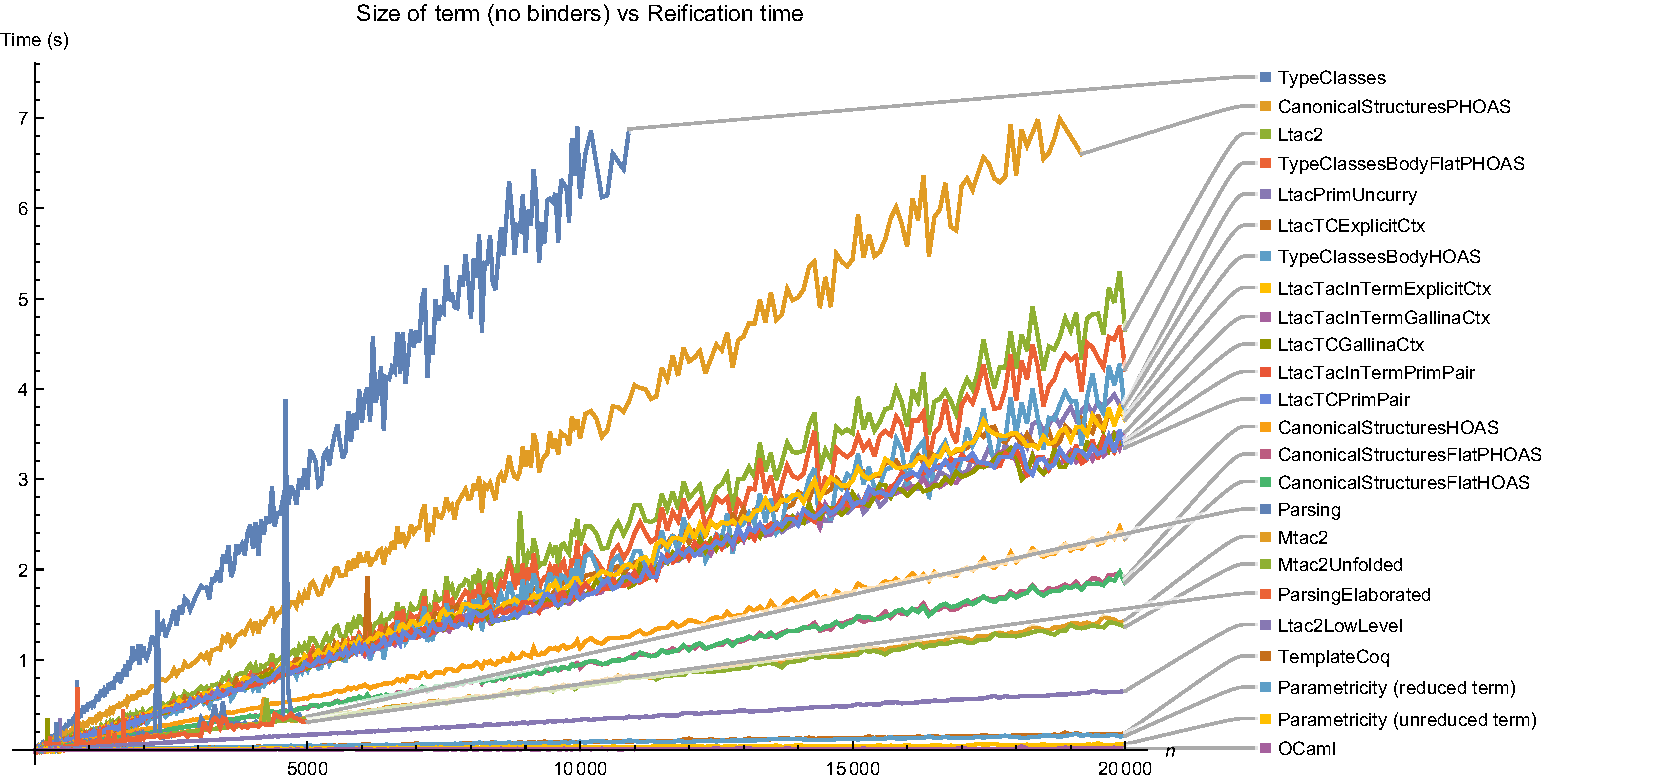
\includegraphics[width=\textwidth]{reification-by-parametricity-outputs/actual-reif-no-binders.pdf}
\caption{Performance of Reification without Binders}\label{fig:graph-reif-no-binders}
\end{figure}

Sorted from slowest to fastest, most of the labels in \autoref{fig:graph-reif-no-binders} should be self-explanatory and are found in similarly named \texttt{.v} files in the associated code; we call out a few potentially confusing ones:
\begin{itemize}
  \item
    The ``Parsing'' benchmark is ``reification by copy-paste'': a script generates a \texttt{.v} file with notation for an already-reified term; we benchmark the amount of time it takes to parse and typecheck that term.
    The ``ParsingElaborated'' benchmark is similar, but instead of giving notation for an already-reified term, we give the complete syntax tree, including arguments normally left implicit.
    Note that these benchmarks cut off at around 5000 rather than at around 20\,000, because on large terms, Coq crashes with a stack overflow in parsing.
    %For size reasons, we do not include these \texttt{.v} files in the associated code tarball, but they can be made via the \texttt{parsing-test-files} target, which generates some files in \texttt{Benchmarks/}.
%  \item
%    In \autoref{sec:ltac2-reif} we mention both a naïve transcription of \Ltac1 to \Ltac2 and a procedure using low-level primitives in \Ltac2; ``Ltac2'' benchmarks the former, and ``Ltac2LowLevel'' benchmarks the latter.
  \item
    We have four variants starting with ``CanonicalStructures'' here.
    The Flat variants reify to \texttt{@expr nat} rather than to \texttt{forall var, @expr var} and benefit from fewer function binders and application nodes.
    The HOAS variants do not include a case for \letindots\space nodes, while the PHOAS variants do.
    Unlike most other reification methods, there is a significant cost associated with handling more sorts of identifiers in canonical structures.
\end{itemize}

We note that on this benchmark our method is slightly faster than template-coq, which reifies to de Bruijn indices, and slightly slower than the quote plugin in the standard library\footnote{This plugin no longer appears in this graph because it was removed in Coq 8.10~\cite{coq-pr-remove-quote-plugin}, though it appears in the graph in \textcite{reification-by-parametricity}.} and the OCaml plugin we wrote by hand.

\subsection{With Binders} \label{sec:perf:binders}

We look at terms of the form \texttt{dlet a$_1$ := 1 * 1 in dlet a$_2$ := a$_1$ * a$_1$ in \ldots\space dlet a$_n$ := a$_{n-1}$ * a$_{n-1}$ in a$_n$}, where $n$ is the size of the term.
The first graph shown here includes all of the reification variants at linear scale, while the next step zooms in on the highest-performance variants at log-log scale.

\begin{figure}[t]
\noindent 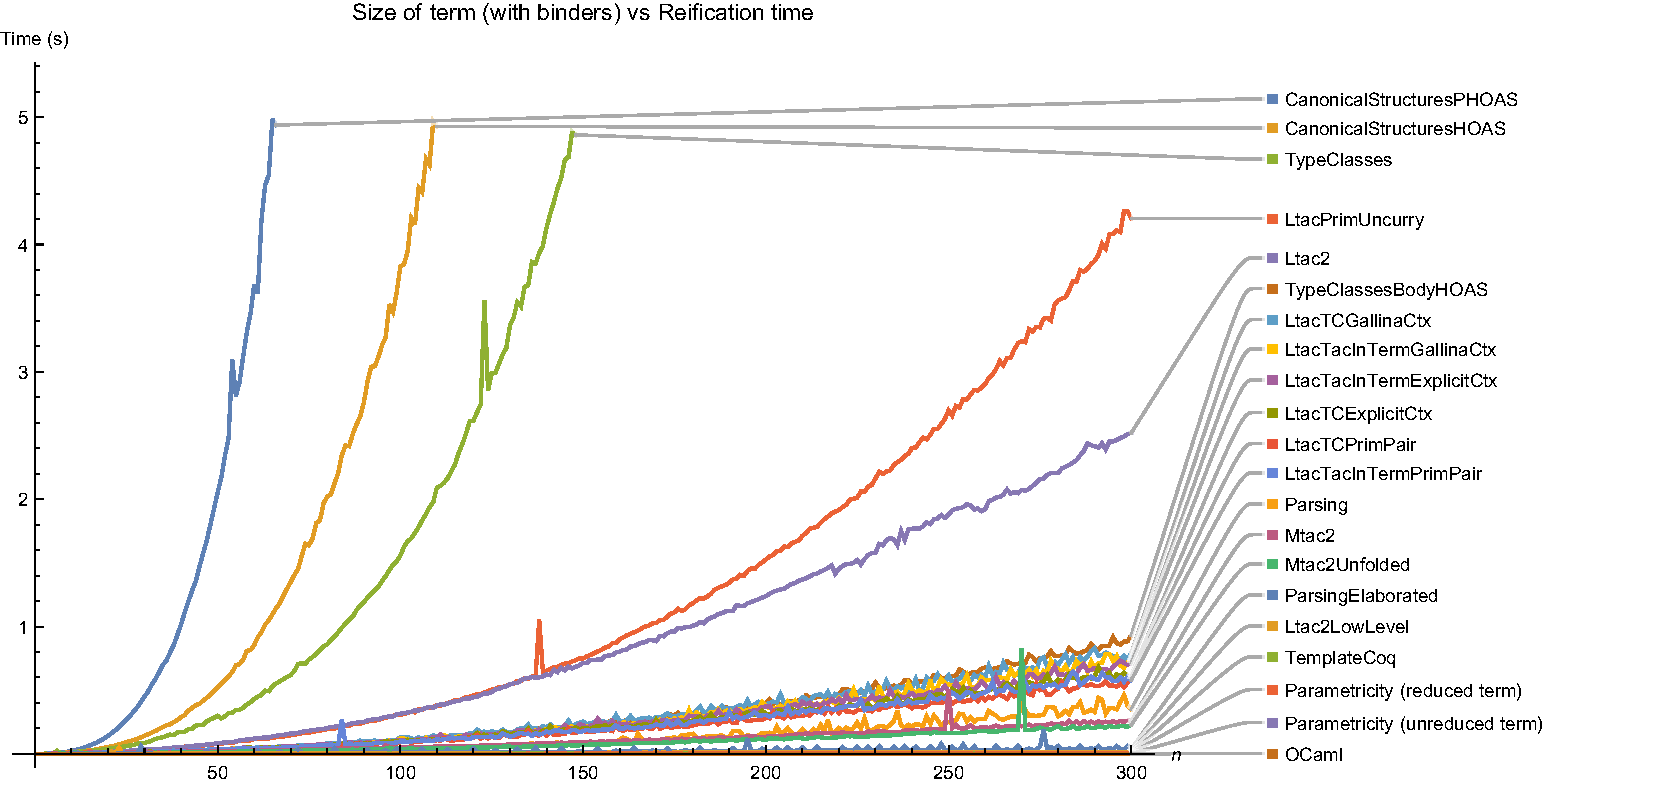
\includegraphics[width=\textwidth]{reification-by-parametricity-outputs/actual-reif-with-binders.pdf}

\noindent 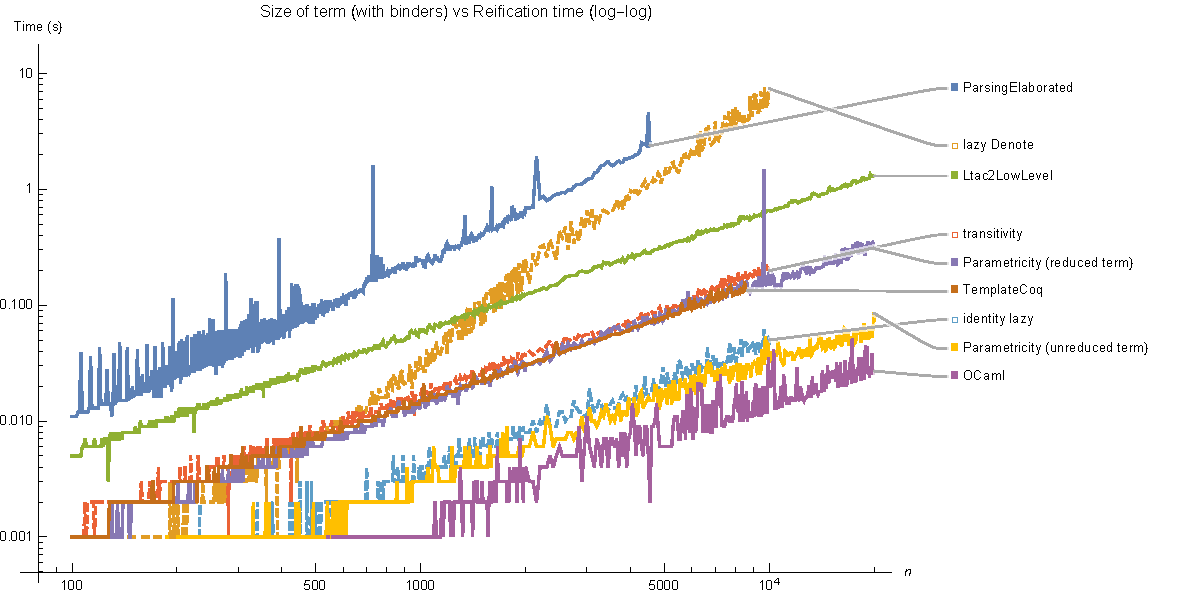
\includegraphics[width=\textwidth]{reification-by-parametricity-outputs/actual-reif-with-binders-log-log-subset.pdf}
\caption{Performance of Reification with Binders}\label{fig:reif-binders}
\end{figure}

In addition to reification benchmarks, the graph in \autoref{fig:reif-binders} includes as a reference (1) the time it takes to run \texttt{lazy} reduction on a reified term already in normal form (``identity lazy'') and (2) the time it takes to check that the reified term matches the original native term (``lazy Denote'').
The former is just barely faster than OCaml reification; the latter often takes longer than reification itself.
The line for the template-coq plugin cuts off at around 10\,000 rather than around 20\,000 because at that point template-coq starts crashing with stack overflows.

\todo{is this still true?}
A nontrivial portion of the cost of ``Parametricity (reduced term)'' seems to be due to the fact that looking up the type of a binder is linear in the number of binders in the context, thus resulting in quadratic behavior of the retyping step that comes after abstraction in the \texttt{pattern} tactic.
In Coq 8.8, this lookup is $\log n$, and so reification has become even faster than the plots indicate~\cite{coq-pr-fast-rel-lookup}.

\section{Future Work, Concluding Remarks} \label{sec:future}

We identify one remaining open question with this method that has the potential of removing the next largest bottleneck in reification: using reduction to show that the reified term is correct.

\begin{wrapfigure}[11]{r}{9cm}
%\vspace{-36pt}
\[
\xymatrix@R=0.5em@C=0em{
    \txt{unreduced term} \ar[d]^{\delta} \\
    \txt{small partially \\ reduced term}
    \ar@<1ex>[ddr]
    \ar@<-1ex>@{--}[rr]
    &&
    \txt{unreduced \\ reified syntax}
    \ar@<-1ex>@{--}[ll]^{???}
    \ar@<1ex>[ddl]
    \\ \\
    &
    \txt{unreduced \\ abstracted term}
    \ar@<1ex>[uul]
    \ar@<1ex>[uur]%^{\rotatebox{40}{\llap{\text{application\hspace*{-2em}}}}}
}
\]
%\vspace{-18pt}
\caption{Completing the commutative triangle}\label{fig:reify-denote-parametricity}
\end{wrapfigure}
Recall our reification procedure and the associated diagram, from \autoref{sec:expanded-reif-diagram}.
We perform $\delta$ on an unreduced term to obtain a small, partially reduced term;
we then perform abstraction to get an abstracted, unreduced term, followed by application to get unreduced reified syntax.
These steps are all fast.
Finally, we perform $\beta\iota$-reduction to get reduced, reified syntax and perform $\beta\iota\delta$ reduction to get back a reduced form of our original term.
These steps are slow, but we must do them if we are to have verified reflective automation.

It would be nice if we could prove this equality without ever reducing our term.
That is, it would be nice if we could have the diagram in \autoref{fig:reify-denote-parametricity}.

The question, then, is how to connect the small partially reduced term with \texttt{denote} applied to the unreduced reified syntax.
That is, letting $F$ denote the unreduced abstracted term, how can we prove, without reducing $F$, that
\[
F\ \mathbb{N}\ \text{Mul}\ \text{O}\ \text{S}\ (\text{@Let\_In }\mathbb{N}\texttt{ }\mathbb{N})
=
\texttt{denote}\ \left(F\ \texttt{expr}\ \texttt{NatMul}\ \texttt{NatO}\ \texttt{NatS}\ \texttt{LetIn}\right)
\]

We hypothesize that a form of internalized parametricity would suffice for proving this lemma.
In particular, we could specialize the type argument of $F$ with $\mathbb N \times \texttt{expr}$.
Then we would need a proof that for any function $F$ of type
\[
\forall (T : \texttt{Type}), (T \to T \to T) \to T \to (T \to T) \to (T \to (T \to T) \to T) \to T
\]
and any types $A$ and $B$, and any terms $f_A : A \to A \to A$, $f_B : B \to B\to B$, $a : A$, $b : B$, $g_A : A \to A$, $g_B : B \to B$, $h_A : A \to (A \to A) \to A$, and $h_B : B \to (B \to B) \to B$, using $f\times g$ to denote lifting a pair of functions to a function over pairs:
\begin{align*}
  & \texttt{fst}\ \left(F\ (A \times B)\ (f_A \times f_B)\ (a, b)\ (g_A \times g_B)\ (h_A \times h_B)\right) = F\ A\ f_A\ a\ g_A\ h_A \;\wedge \\
  & \texttt{snd}\ \left(F\ (A \times B)\ (f_A \times f_B)\ (a, b)\ (g_A \times g_B)\ (h_A \times h_B)\right) = F\ B\ f_B\ b\ g_B\ h_B
\end{align*}
This theorem is a sort of parametricity theorem.

Despite this remaining open question, we hope that our performance results make a strong case for our method of reification; it is fast, concise, and robust.

\part{Conclusion}
\chapter{Tooling fixes (improvements in Coq)} \label{ch:coq-tooling-fixes}


\begin{subappendices}
    \section{Fragments from the category theory paper}
    For reasons that we present in the course of the paper, we were unsatisfied with the feature set of released Coq version 8.4.  We wound up adopting the Coq version under development by homotopy type theorists~\cite{HoTT/coq}, making critical use of its stronger universe polymorphism (\autoref{sec:category-of-categories}) and higher inductive types (\autoref{sec:hit}).  We hope that our account here provides useful data points for proof assistant designers about which features can have serious impact on proving convenience or performance in very abstract developments.  The two features we mentioned earlier in the paragraph can simplify the Coq user experience dramatically, while a number of other features, at various stages of conception or implementation by Coq team members, can make proving much easier or improve proof script performance by orders of magnitude, generally by reducing term size (\autoref{sec:term-size}): primitive record projections (\autoref{sec:prim-record-proj}), internalized proof irrelevance for equalities (\autoref{sec:equality-reflection}), and $\eta$ rules for records (\autoref{sec:no-judgmental-eta}) and equality proofs (\autoref{sec:compute-match}).
    
    \hrule
    
    
    \section{transcript bits from Adam}
    Ah a sort of like preconclusion chapter that's like let's now look at how cock is evolved performance wise over the years like here places that we've actually improved performance and this will be one that draws a bunch of other examples from the category theory paper, like look universe polymorphism is a thing that was implemented and helps here and like sort of like presenting a bunch of little things. 
\section{transcript bits from Rajee}
So those are the two main sections the thesis. And then there's another section of other small. Miscellaneous things that come up better like performance bottlenecks. Through like can or performance concerns, let's say these are things like decide design decisions that can have quadratic impacts. Um, Decisions about like what parts of cop to use for what and like why some bits might be more or less slow than others. 

Yeah, that's that's that section and then I think I'm going to have seconds last section. Be a sort of retrospective of like places where cocks performance has gotten better in the past like decade or so of like I started with a bunch of ways that solving performance issues improved systems is heard but here are some successes and things where like we've managed to improve things and you can actually like, Leverage this for faster performance. 


\todo{this chapter}
\end{subappendices}
\chapter{Concluding Remarks}

\begin{subappendices}
    
    \section{transcript bits from Adam}
And then they'll be the conclusion which I'm thinking of having as a like what are the next steps in performance of previous distance and I think this will. My current inclination is to like, Sort of point towards the paper that under has been talking about writing that's like okay, so there's a sense in which in order to do program transformation and rewriting we took the entire non-trusted part and we threw it out. 

The like. And like part of that is because most uses of the non-trusted part you just cobble something together that works but if you're like tracking every single time you invoke conversion and you're like carefully piecing together something it should be possible to make something that scales. And it's not clear if that's currently even the case. 

Unlike investigating that it's sort of the next wave of. Performance issues to look at. Okay. Well when you get to the conclusion of this sort of document you've pretty freehand to speculate on things and go where your heart takes you so I'm not too worried about I haven't feel like that part of the relatively quick for you to write and free of difficult choice points. 

Yeah, that seems that seems mostly true. I feel like I'll have a little bit of trouble with the like first paragraph on the last paragraph of the conclusion. I'd like the transition points and they'll like actually tying it up but the body of it seems I don't expect to have that much trouble, okay? 

    
    \section{transcript bits from Rajee}

\todo{Decide between options, maybe add more text}
\paragraph{Option 1}
Perhaps this thesis has inspired you to write your own performance system and we remind you about the things you should look out for when implementing it. 

\paragraph{Option 2}

The End

\todo{insert category theory diagram of an End here}

\paragraph{Option 3 (best so far)}

What are the next steps in proof assistant performance.  There's a paper that Andres has floated writing that I think is a good next paper to write. 

Ah, that is something like okay, so you've like, Followed all the tenants that I've laid out to like have fast APIs you're like very careful about where you're having called two things. And then you start hitting so brief historical perspective. I've described a bunch of like quadratic or exponential behaviors where like you're hitting. 

Areas of the system that aren't scaling nicely. There was a previous generation to this where pretty much everything was quadratic or exponential in like everything and so you couldn't do anything beyond a certain scale because everything would start blowing up on you I see and there was someone before me named George got there who when working on he was the one who led the team at Microsoft Research to you formalized the four color theorem. 

I think now not the four color theorem the odd order theorem. In call okay took them about ten years. I think you've mentioned this yeah oh and he went on the cocktails and they fixed these like everything is terrible and everything. So now we're heading like problems that maybe maybe are more fundamental to proof assistance. 

But like then you you design your things carefully and you're careful about which parts the system you use and you'd like count for every step. And then you start hitting the next class of problems, which is I have a couple thousand things. A couple thousand variables and I want to introduce them all oops adding a couple thousand like adding n variables is quadratic or cubic in the number of variables that I'm introducing that's unfortunate. 

Um, or you're like I want to like change my goal state oops making a new goal state is linear in how many variables there that's sad now. I'm now by running time is quadratic in the number of goal states or something mm-hmm. 

And like you hit all of these like the fundamental building blocks. Are too slow. And. That's sort of the next area to investigate of like how do you build a proof assistant so like what are the fundamental building blocks? How are they too slow? Huh the how do we know there are two slow what what are the factors that they're too slow and like can we show that there's like no way to get anything to actually scale without completely re-implementing the profanion because that's basically what I what I said for program transformation. 

I'm like look the existing thing it's quadratic it's real sad let's throw it out and write a new one and stick it in the part of the system that's fast. So like yeah, you can do that for all your proofs you can throw out the entire pure system and write a new one. 

But like, Would be nice if you didn't have to do that we say that again. So like you're like, okay, I was trying to do this thing no just the last sentence, oh it would be nice if we didn't have to do that yeah. So the alternative is to the to the alternative is that you figure out what the primitives are what they're too slow and why they're too slow and how do you design a proof assistant like a proof engine with primitives that are actually performant that if you're carefully accounting for all of the primitive steps that you're doing in your proof then you can actually get a proof with reasonable performance. 

Like all the things that I've been describing are. You slap something together and it works on small things and then you increase your you try to scale it and it's suddenly stops working because of exponential behavior. And like, Maybe there isn't a hope of fixing that if you slap something together. 

But if you're like carefully engineering your proof, you should be able to avoid that. What is the careful part like can you describe that or is it just like the thing so? Okay, so here's how here's how beginners pure things in caulk. Their teacher tells them what they're trying to prove. 

They look at what they're trying to prove they look at the list of things they can do they're like, oh I'm trying to prove for all X something. I know a tactic to use. I'm gonna use interest. Oh I'm trying I have a conjunction in my hypothesis that I know a tactic to use I'm gonna use destruct. 

I'm trying to prove something about natural numbers, how do I prove something about natural numbers by induction? Where you have this very simple pattern match that are matching program that's running in a brain that you're like how do I do this thing one step at a time? I'm just gonna try a thing and see what works we have some arithmetic, let's try simple let's see if cock knows how to make it simpler there's a tactic called simple without the, Okay, um, sometimes it makes things much nicer. 

Sometimes it makes things explode, sometimes it runs forever and gives you nothing it doesn't actually ever run forever pretty much. But running for a year is about as good as running forever. 

And so you'll try it and if it works then you're like great it worked. I can keep going yeah and if it doesn't work then you're like, oh I guess it didn't work, let me try something else instead. And like this is this is how beginners implement proofs and like the way I do proofs is I'm like, okay, let me figure out why this thing should be true. 

And let me figure out what gets me closer to my understanding of why it should be true and then I run the same kind of simple program that um that beginners run that's like, oh this should be true by induction on this variable. I'm not just doing induction randomly. 

I know why I'm doing induction on what and I'm like, oh I have this conjunction. I can split it apart. I have this disjunction I can split it apart and like I keep making steps and at each point. I'm like, am I still convinced that this theorem is true? 

And if I have ever I'm like, oh doesn't these seem like this true anymore that I'd like backup but otherwise I just keep going as long as I'm convinced that the theorem is still reasonable. Where you say something like you do things by figuring out why something should be true is that like. 

Is that like constructing approved sketching your head and then doing it versus someone being like oh I know what tactic to implement them, therefore. I will try to construct yeah it's like using a proof method to generate a proof versus knowing what you want to prove and then writing it need to or something oh where is this something different like how does it apply to the engineering case? 

I think it's something like that okay, so the thing that I'm doing is I'm like do I believe that this is true when I explain to a very intelligent five-year-old why this is true. And then I'll make steps unlike if at any point. I hit a theorem that I or like I hit a state where I'm like. 

This is doesn't seem true anymore. That I'll like back up but I and like I have a big sense of the proof in my head okay, oh but it's like I'm like, okay this this should follow by arithmetic. So then I do a bunch of arithmetic like things and eventually hopefully I get out a thing that's true, but it's like if I want to prove that something is true by arithmetic. 

I can just like look at my thing take a step that makes the thing simpler and if the thing still seems true that I'm like great I made it simpler now what and like I can keep taking steps to make it simpler until it's done and I don't have to have a like entire proof in my head. 

That's interesting. Don't yeah yeah, this is because I got lined by line feedback on my prefixes. I go along it's great. Yeah. The problem with doing things this way is that they don't scale yeah it seems hard like. It seemed like I feel like with most problems you have to kind of have a proof in your head and then use the syntax to like. 

Make it so let me let me also clarify yeah the sorts of proofs currently that you need to do in caulk or way simpler and the more tedious and the sorts of proofs that you're thinking of here's an example of a proof that you might have to do in caulk, um, this is this is like on the interesting end of proofs okay, oh if you, Have a loop that adds up all the numbers between one and m. 

It's the same thing as multiplying n times, m, plus one dividing by two, okay? This is the interesting proof here's another interesting proof, we're merged sword and bubble sort give you the same list if you give them the same list then. In both cases do just do it you you prove so the things you need to prove is you need to prove that they're included or do you just run both things and say no you can't run both things because you need to prove that it's true for every single list, right? 

So yeah so the way that you would prove this is you define what it means to be sorted better to be what it means to be a stable sorting of a particular list, maybe you don't need that. I think you can just define what it means to be sorted and what it means for like two lists to be the same up to permutation and you're like for any list there's a unique list, that is the same up to permutation and also sorted. 

Look both of these sorting methods produce that list. Okay, oh and like this is at the interesting end the like standard end or things like, um, 

If I have a binary tree that holds numbers. And I add one to all the leaves then I take the sum of all the leaves. The number that I get is the number of leaves plus the sum of all the leaves before I added one. 

You know, it's these sort of like trivial structural properties. 

A lot of time is that proving trivial structural properties. I see so so it's not like you like there's like a it's often not like you're missing a concept and understanding how to generate the proof or something but you need like an elegant way to like structure the proof or something and that's the part where you're saying that the beginner would just be like here's tactic. 

I will apply it anywhere like oh what's the good structure to do this or something? I mean, even I'm not what's the good structure to this? I'm like what's what's the structure to do this that isn't wrong? Okay, the beginner is like, Like cargo culting Margo what cargo holding that means? 

I maybe it's originated from Richard Feynman and that. There are some places where the. Ah, like livelihood of the tribes depended on like airplane deliveries of cargo. And. Like there was always a ritual associated with the cargo showing up where you like wave the lights in the air so that the airplane can land on the landing strip. 

And so you can like there there were some cults so I hear I don't know how accurate this is that developed around this where people would waive the lights in the air hoping that this would make the airplanes in the cargo show up. I see right so you can do the same sort of thing with programming you're like, oh I found the program that does the thing. 

I want maybe I can take the code and maybe it'll do the thing. I want. And like you'll also include all the other care and like you're like, why is this other code here? Well, because it was in this other program that did the thing that I want. I don't know if I need it. 

So like why are you doing this proof like this because the example proof that I saw had this structure and it worked through the system was like, okay. Yeah, right. So I am I'm at a more advanced level where I'm like, okay, I know that's a proof things about binary trees. 

I'm gonna go by induction on the binary tree and I'll do something with the number of leaves and I'll figure the rest of the details out as I go. 

And this is how most proofs get done. You do them piecewise. And you like don't account for like how much work call has to do at each step, you're like try it. So work it works then it's good doesn't work that it's bad. And like you could carefully in your head design the entire proof and like carefully account for how much work you expect cock to have to do at each step and make sure that cock shouldn't have to do any work that you don't think it should do. 

But very few people designed proofs like this. But it should be possible to get a proof that is fast if you design it like this and like the next wave of performance issues is going to be that even when you're designing proofs like this things are still not fast enough. 

And so then that's Cox problem. That's the like, how do you design a proof assistant with good enough primitives? Right, yeah, right. I'm like, look you can just. Throughout throw out the prevention. Do this other thing instead works nicely. 

But like it would be nice if you don't have to do that. To get things to scale. 

And yeah, that's that's the sort of next step. Right. Now, that's not like a nicer conclusion. Next step is all these very inspiring. 

\end{subappendices}

\appendix
%\include{appa-selected-code}
%\include{appb}
%% This defines the bibliography file (main.bib) and the bibliography style.
%% If you want to create a bibliography file by hand, change the contents of
%% this file to a `thebibliography' environment.  For more information
%% see section 4.3 of the LaTeX manual.
\begin{singlespace}
%\bibliography{references}
%\bibliographystyle{plain}
\nocite{*}
\printbibliography
\end{singlespace}

\end{document}
